%%%%%%%%%%%%%%%%%%%%%%%%%%%%%%%%%%%%%%%%%%%%%%%%%%%%%%%%%%%%%%%%%%%
%                                                                 %
%                            ROOT FILE        5                    %
%                                                                 %
%%%%%%%%%%%%%%%%%%%%%%%%%%%%%%%%%%%%%%%%%%%%%%%%%%%%%%%%%%%%%%%%%%% 

\documentclass{report}
% \pdfminorversion=6 %%CHECK WITHOUT IT AT THE END
%%%%%%%%%%%%%%%%%%%%%%%%%%%%%%%%%%%%%%%%%%%%%%%%%%%%%%%%%%%%%%%%%%%%%%%%%%%%
% preamble

% graphics
\usepackage[pdftex]{graphicx}
%\usepackage{pdfsync}  %%DANGER!!! for inverse search only. Disable when document is ready!
\graphicspath{{Figures/}}
\DeclareGraphicsExtensions{.pdf,.jpg}

\usepackage{enumerate}
\usepackage{amssymb}
% \usepackage{amsmath}

% headers and footers
\usepackage{fancyhdr}
\pagestyle{fancy}
\renewcommand{\chaptermark}[1]{\markboth{\chaptername \ \thechapter.\ #1}{}}
\renewcommand{\sectionmark}[1]{\markright{\thesection.\ #1}{}}
\renewcommand{\headrulewidth}{1pt}
%\fancyhead{}
\fancyhead[LE,RO]{\sc \footnotesize \rightmark}
\fancyhead[LO,RE]{\sc \footnotesize \leftmark}
\fancyfoot[C]{\thepage}

% problem and example numbering
\newtheorem{problem}{Problem}[chapter]
\newtheorem{example}{Example}[chapter]
\newtheorem{definition}{Definition}[chapter]
\newtheorem{theorem}{Theorem}[chapter]

%definitions
\newcommand{\rdots}{\mathinner{%
  \mkern1mu\raise1pt\hbox{.}%
  \mkern2mu\raise4pt\hbox{.}%
  \mkern2mu\raise7pt\vbox{\kern7pt\hbox{.}}\mkern1mu}}

\def\matnotation4#1#2#3#4{
\matrix{ #1\cr #2\cr #3\cr #4\cr }}

\def\threevec#1#2#3{
\left[\matrix{ #1\cr #2\cr #3\cr }\right]}

\def\twovec#1#2{
\left[\matrix{ #1\cr #2\cr }\right]}
\def\lrarr{\leftrightarrow}
\def\rarr{\rightarrow}
\def\aa{{\bf a}}
\def\bb{{\bf b}}
\def\cc{{\bf c}}
\def\dd{{\bf d}}
\def\xx{{\bf x}}
\def\zv{{\bf 0}}
\def\rr{{\bf r}}
\def\vv{{\bf v}}
\def\xx{{\bf x}}
\def\qq{{\bf q}}
\def\rr{{\bf r}}
\def\vv{{\bf v}}
\def\xx{{\bf x}}
\def\yy{{\bf y}}
\def\qq{{\bf q}}
\def\pp{{\bf p}}
\def\eee{{\bf e}}
\def\ii{{\bf i}}
\def\jj{{\bf j}}
\def\kk{{\bf k}}
\def\RR{{\bf R}}
\def\zz{{\bf z}}
\def\yy{{\bf y}}
\def\PA{\partial}

\begin{document}
\tableofcontents
	
\chapter{Introduction}

Linear Algebra is a branch of Mathematics. Many applied problems from
Science, Engineering and Finance can be written in terms of Linear
Algebra questions. This is also true of Calculus, which is why these
two fields are stressed in undergraduate Mathematics education at UBC
and other universities. By putting a class of commonly occurring
problems into a unified, abstract framework, the problems can be
studied in detail and well understood. This understanding can then be
taken back to problems in many different fields. It is especially
important to realize that very large problems (with potentially
millions of unknowns) can be understood in the same framework as the
model problems we do by hand in these courses. This course has
computer labs that involve the mathematical software, MATLAB, that
will allow you to solve larger problems using numerical computations. 

Unlike Calculus, Linear Algebra does not require a lot of background
knowledge. Basic operations in Linear Algebra are just
arithmetic. However, there is a powerful connection between these
simple arithmetic operations and geometric quantities. Simple ideas in
this course start to become abstract when combined together. Linear
Algebra is a subject you can study with very limited matematical 
background, but
you are advised to keep up with course lectures, readings, assignments
and computer labs so you won't be left behind at the transition from
concrete ideas to abstract ones.

\section{Course Goals}

The goal of the course is to enable students to 
\begin{enumerate}
\item recognize linear algebra questions (for which there are
straight-forward analytic and numerical solution techniques) as parts
of applied problems
\item make the connection between geometric properties and analytic
quantities (determinants, dot and cross products, eigenvalues, etc.)
\item recognize that linear systems of equations can have unique,
infinite or no solutions and know how to determine all solutions or
that none exist
\item recognize matrix multiplication as a linear transformation and
that such transformations (to the same dimensional space) can be
simplified using eigen-analysis
\item use complex numbers, which arise naturally in the eigen-analysis
of matrices
\end{enumerate}

\section{About the Subject} 

The subject of the course is Linear Algebra, focussing on four main
topics: 
\begin{enumerate}
\item vectors and matrices and connections to geometry
\item linear systems
\item complex numbers 
\item eigen-analysis of matrices
\end{enumerate} 
Several applications are considered. The two applications that come up repeatedly in the notes are resistor networks and random walks. 

\subsection{Connection to Geometry}

The first topic considered in the course is vectors, which are
quantities with both magnitude and direction. A typical quantity
represented as a vector is a force $\bf F$ on an object as shown in
Figure~\ref{fig_intro1}. The force $\bf F$ in that figure acts in the
$x-y$ plane as shown. The vector force $\bf F$ can be represented by
its components $(F_x, F_y)$. Some interesting questions you will be
able to answer after completing this course are: what directions are
perpendicular to this force?; what are the coordinates of the force in
the rotated coordinate system $x^\prime - y^\prime$?; what are the
coordinates of the force if its direction is rotated? These last two
questions are related.
\begin{figure}
\centerline{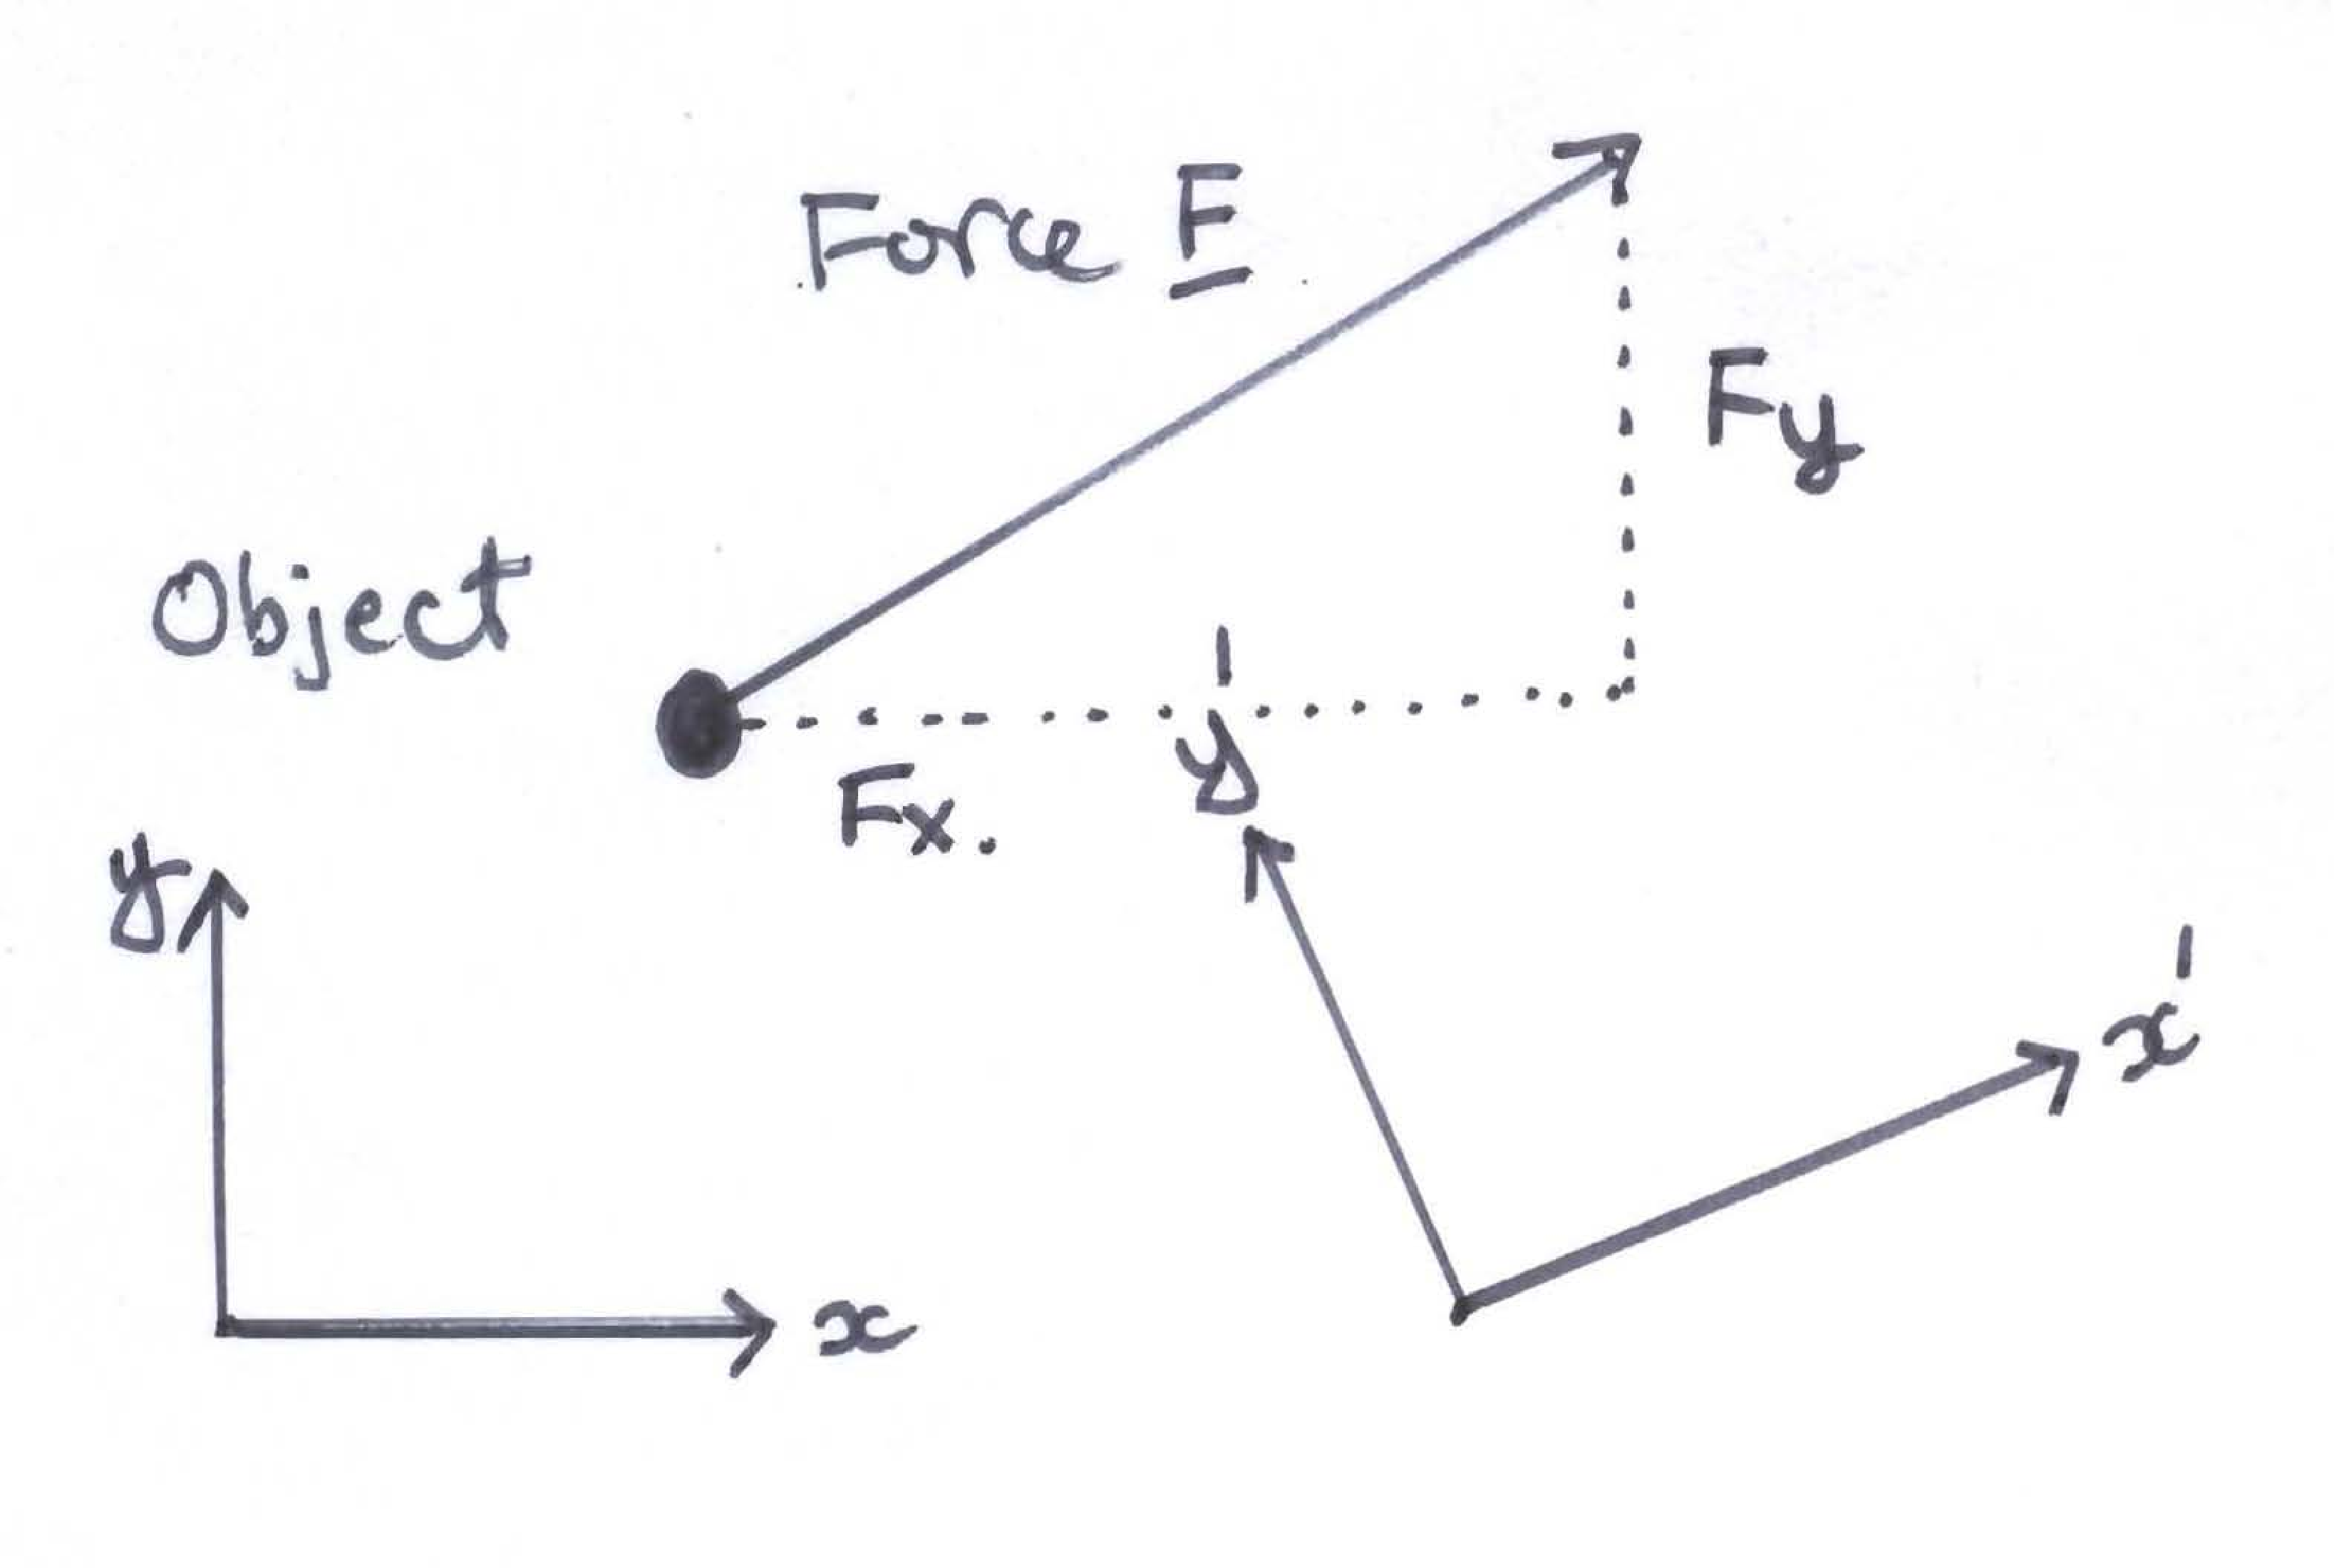
\includegraphics[height=4cm]{1_introfig1}}
\caption{\label{fig_intro1} Force vector and coordinate systems.}
\end{figure}

\subsection{Linear Systems}

Consider the following simple example. You probably saw something like
this in high school. 

\begin{example} Bob and Sue together have 12 dollars. Sue has
2 dollars more than Bob. How much money do each have? 
{\rm You can probably guess the solution by trial and error, but let us
proceed a bit more formally. Let $x$ be the amount of money Sue has
and $y$ the amount Bob has. The two statements in the example can be
written mathematically as
\begin{eqnarray*}
x + y & = & 12 \\
x - y & = & 2.
\end{eqnarray*}
The equations above are a {\em linear system} for the unknowns $x$ and
$y$. A technique that can be used to solve the system (that is,
determine the values of $x$ and $y$ that {\em simultaneously} solve
both equations above) is substitution. The second equation can be
written as
\[
x = y+2
\]
This can be substituted into the first equation above, {\em
eliminating} $y$ from the problem
\[
(y+2) + y = 12 \mbox{\   or $2y +2 = 12$ \ so $2y = 10$ \ so $y=5$}
\]
The value of $y=5$ determines $x=7$ from either of the original
relationships. Thus it is determined that Bob has 5 dollars and Sue
has 7. }
\end{example}

Often (but not always) a linear system of $n$ equations for $n$
unknowns has a unique solution. The example above was for the case
$n=2$. However, the substitution technique used above becomes
impractical when $n$ is larger than 3. In this course you will learn
the Gaussian Elimination technique to solve linear systems. This
systematic method can find all solutions when there are any and also
determine if the system has no solutions. This method can be
implemented in numerical software and used to solve very large
systems.

\subsection{Eigen-analysis} 

The final subject of the course is eigen-analysis of matrices and its
applications. A simple, motivational example comes from the study of
discrete dynamical systems. Consider a sequence of values 
\[
x_0, x_1, \cdots x_n \cdots
\]
where the index $n$ is a time level. Suppose that $x_n$ is determined
by the previous value $x_{n-1}$ in the same way for every $n$, that is
\begin{equation}
\label{eq:intro1}
x_n = f(x_{n-1}) \mbox{\ \ for every $n \geq1 $} 
\end{equation}
for a given function $f$. This could describe the population number $x_n$
of a species at year $n$. The simple model assumes that the population 
the next year only depends on the population this year through the 
function $f$. 
If the initial value $x_0$ were given, then
the values $x_1, x_2 \cdots x_n \cdots$ could be determined using
(\ref{eq:intro1}) repeatedly. A linear problem arises when we take the
specific example $f(x) = ax$ where $a$ is a given constant. In this
case, it is easy to compute the entries of the sequence:
\begin{eqnarray*}
x_1 & = & f(x_0) = a x_0 \\ 
x_2 & = & f(x_1) = f(a x_0) = a^2 x_0 \\ 
\vdots & & \vdots \\
x_n & = & f(x_{n-1})) = a^n x_0
\end{eqnarray*}
For this example, we can determine how the sequence behaves very well
because we have an expression for $x_n$ above that is easy to
understand. There are several cases:
\begin{enumerate}
\item If $x_0 = 0$ then $x_n =0$ for all $n$. 
\item if $|a|< 1$ then $\lim_{n \rightarrow \infty} x_n = 0$.
\item if $a=1$ then $x_n = x_0$ for all $n$.
\item if $a=-1$ then the values alternate in sign: $x_n$ has the value
$x_0$ is $n$ is even, $-x_0$ if $n$ is odd.
\item if $|a|>1$ and $x_0 \neq 0$ then the values of the sequence grow
in absolute value as $n \rightarrow \infty$.
\end{enumerate}

Linear discrete dynamical systems for vectors are also of interest. In
these cases, multiplication by the number $a$ in the example above is
replaced by multiplication by a matrix $\bf A$. Eigen-analysis of the
matrix $\bf A$ allows one to understand how the system behaves as $n
\rightarrow \infty$ in a similar way to the simple example above. Eigen-analysis naturally involves complex arithmetic, so this is introduced in the notes beforehand. 

\section{About The Computer Labs}

The course includes six one-hour computer labs. These are given to
small groups of students every other week starting in the {\em second}
week of the term. It is a good idea
to read through the lab notes before going to the lab so you are ready
to begin in the lab. After your first lab, you will be able to go to
the lab rooms in open hours to improve your MATLAB skills and to
prepare for upcoming labs. Computer lab material including your knowledge
of MATLAB commands will be tested on midterms and the final exam. 

There are two main goals for the labs. The first is to gain
familiarity with the computational tool, MATLAB, that is commonly used
in later courses and Engineering careers. The second is to be able to
solve larger, more interesting applied problems that would otherwise
be inaccessible using analytic methods. Seeing the algorithms of
MATLAB in action may also help you understand the underlying
mathematical concepts you see in the lectures.

\section{About These Notes}

\begin{description}
\item[2004:] 
The first version of these notes was written by Richard Froese for
Math 152 taught in the Spring of 2004. There are many text books on
elementary linear algebra material, but none have the material in the
order we want for Math 152 for Applied Science students. These notes
stress geometric concepts in two and three dimensional space. They
also treat applications and numerical approximation using MATLAB in
more detail than most texts. For this reason, the authors have felt it
was worthwhile to maintain and improve these notes for Math
152. Additionally, we believe it is a social benefit for students to
have access to this material without having to purchase an expensive,
commercial text.
\item[2007:] 
An update to the notes was made by Richard Froese for the course in
2007, including solutions to the exercises. 
\item[2009:] The version written for
the 2009 course had some updates by Brian Wetton: this introductory
chapter, some additional comments on MATLAB commands, a reworked
section on linear systems arising from electrical networks, and
additional problems and solutions. In addition, the notes were 
converted to standard \LaTeX format to make them easier to maintain. 
\item[2010:] 
Substantial revisions for the notes for 2010 were done by Ignacio Rozada, who was supported 
by a UBC Skylight grant over the Summer of 2009 to add the problems 
and solutions used in weekly assignments the previous year. He also 
added additional MATLAB material. Brian Wetton added additional notes 
to Chapter 4 on the use of matrix multiplication and inverses in the 
derivation of solutions to the ``fundamental problem" of resistor 
networks.
\item[2015:] Brian Wetton added many additional examples to Chapter 2 and added more formal 
definitions of the key concepts: linear combination, span, linear independence, basis and dimension. He also added material in Chapter 5 on the use of complex arithmetic in complex linear systems and determinants. 
Joel Feldman contributed an additional topics section to Chapter 3 on the checksum technique. 
Hand drawn resistor network diagrams were replaced throughout the text by Egor Dontsov. The material on 
complex numbers was split off into a separate chapter.
\item[2017:] Brian Wetton corrected errors in the notes pointed out by the 2016 class and added a discussion in the first section of Chapter 4 on the interpretation of matrix vector multiplication as a linear combination of the columns of the matrix.
\item[2025:] Colin B. Macdonald started tracking changes in a Git repo,
posted these notes to GitHub, and fixed some typos.
\end{description} 
Further revisions are planned. There will be additional MATLAB
material added to the notes and additional problems and solutions. The Chapter on complex numbers needs some revision.
If you have any suggestions for additional
material or ways to improve the presentation, please contact the maintainers
at
{\tt https://github.com/UBCMath/Math152notes}


% \end{document}

\chapter{Vectors and Geometry}

%%%%%%%%%%%%%%%%%%%%%%%%%%%%%%%%%%%%%%%%%%%%%%%%%%%%%%%%%%%%%%%%%%%%%%%%%%%%

\section{Chapter Introduction}

This chapter contains an introduction to vectors, which correspond to
points in two, three and higher dimensional spaces. In this chapter,
you will become familiar with basic vector operations such as
addition, scalar multiplication, length, the dot product, and the
cross product (for three dimensional vectors). Vector representation
of lines in 2D and 3D and planes in 3D are presented. Criteria for when
such objects intersect at unique points is given in terms of
determinants. This geometric presentation motivates our study of these
kind of problems in higher dimensional settings in later
chapters. Throughout this chapter, MATLAB commands are introduced that
perform the operations described in the text. For 2D and 3D problems,
using MATLAB is only a convenience. For higher dimensions, doing the
computations by hand (even with a calculator) is impractical, and a
computational framework like MATLAB is essential to be able to solve
these problems.

%%%%%%%%%%%%%%%%%%%%%%%%%%%%%%%%%%%%%%%%%%%%%%%%%%%%%%%%%%%%%%%%%%%%%%%%%%%%

\section{Vectors}

Vectors are used to describe quantities that have both a magnitude and
a direction. You are probably familiar with vector quantities in two
and three dimensions, such as forces and velocities.

Later in this course we will see that vectors can also describe the
configuration of a mechanical system of weights and springs, or the
collections of voltages and currents in an electrical circuit.  These
more abstract vector quantities are not so easily visualized since
they take values in higher dimensional spaces.

We begin this course by discussing the geometry of vectors in two and
three dimensions.  In two and three dimensions, vectors can be
visualized as arrows. Before we can draw a vector, we have to decide
where to place the tail of the vector.  If we are drawing forces, we
usually put the tail of the vector at the place where the force is
applied. For example, in Figure~\ref{fig_pend} (left) 
the forces acting on a pendulum
bob are gravity and the restraining force along the shaft.

\begin{figure}
\centerline{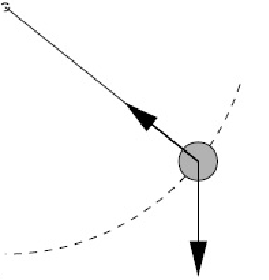
\includegraphics[height=1.5in]{2_pend}
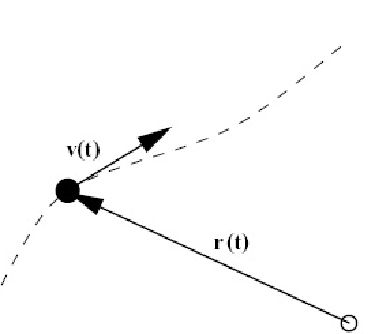
\includegraphics[height=1.5in]{2_velocity}}
\caption{Forces acting on a pendulum (left) and 
position and velocity of a particle (right) \label{fig_pend}}
\end{figure}

If we are drawing the velocity of a particle at a given time, we would
place the tail of the velocity vector ${\bf v}(t)$ at the position of
the particle at that time as shown in Figure~\ref{fig_pend} (right). 
Once we have chosen a starting point for the tails of our vectors
(i.e., an origin for space), every point in space corresponds to
exactly one vector, namely the vector whose tail is at the origin and
whose head is at the given point. For example, in Figure~\ref{fig_pend} 
(right)
we have chosen an arbitrary point as the origin (marked with a circle)
and identified the position of the particle with the vector ${\bf
r}(t)$.

\subsection{Multiplication by a number and vector addition}

There are two basic operations defined for vectors. One is
multiplication of a vector by a number (also called scalar
multiplication). The other is addition of two vectors.

A vector $\aa$ can be multiplied by a number (or scalar) $s$ to
produce a new vector $s\aa$. If $s$ is positive then $s\aa$ points in
the same direction as $\aa$ and has length $s$ times the length of
$\aa$. This is shown in Figure~\ref{fig_scalarmult}.
If $s$ is negative then $s\aa$ points in the direction opposite
to $\aa$ and has length $|s|$ times the length of $\aa$.

\begin{figure}
\centerline{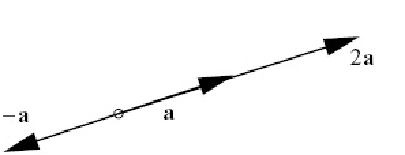
\includegraphics[height=1.5in]{2_scalarmult}}
\caption{Scalar multiplication. \label{fig_scalarmult}}
\end{figure}

To add two vectors $\aa$ and $\bb$ and we draw the parallelogram that
has $\aa$ and $\bb$ as two of its sides as shown in Figure~\ref{fig_add}. 
The vector $\aa + \bb$ has
its tail at the origin and its head at the vertex of the parallelogram
opposite the origin. Alternatively we can imagine sliding (or
translating) one of the vectors, without changing its direction, so
that its tail sits on the head of the other vector. (In the diagram we
translated the vector $\aa$.) The sum $\aa + \bb$ is then the vector
whose tail is at the origin and whose head coincides with the vector
we moved.

\begin{figure}
\centerline{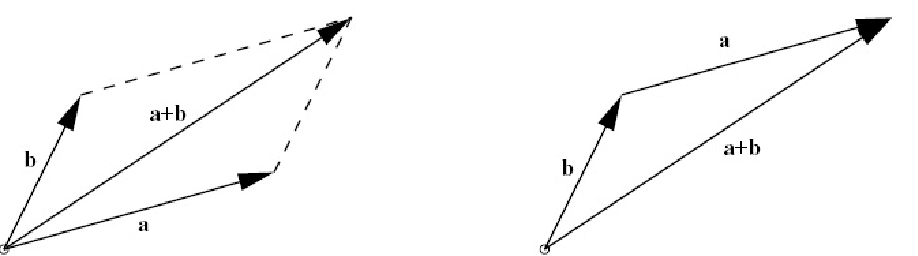
\includegraphics[height=1.5in]{2_add}}
\caption{Vector Addition. \label{fig_add}}
\end{figure}

\begin{example}
\label{2009_a1_3}
Describe and sketch the following set of points $\{ s {\bf a} :
s \in \mathbb{R} \}$ (that is, the set of all scalar multiples of $\bf a$) where
$\bf a$ is a non-zero vector in $\mathbb{R}^2$. {\rm The set is a straight line 
going through the origin with direction $\bf a$ as shown in 
Figure~\ref{ch2exnew1}.}
\end{example}

\begin{figure}[htb]
\centerline{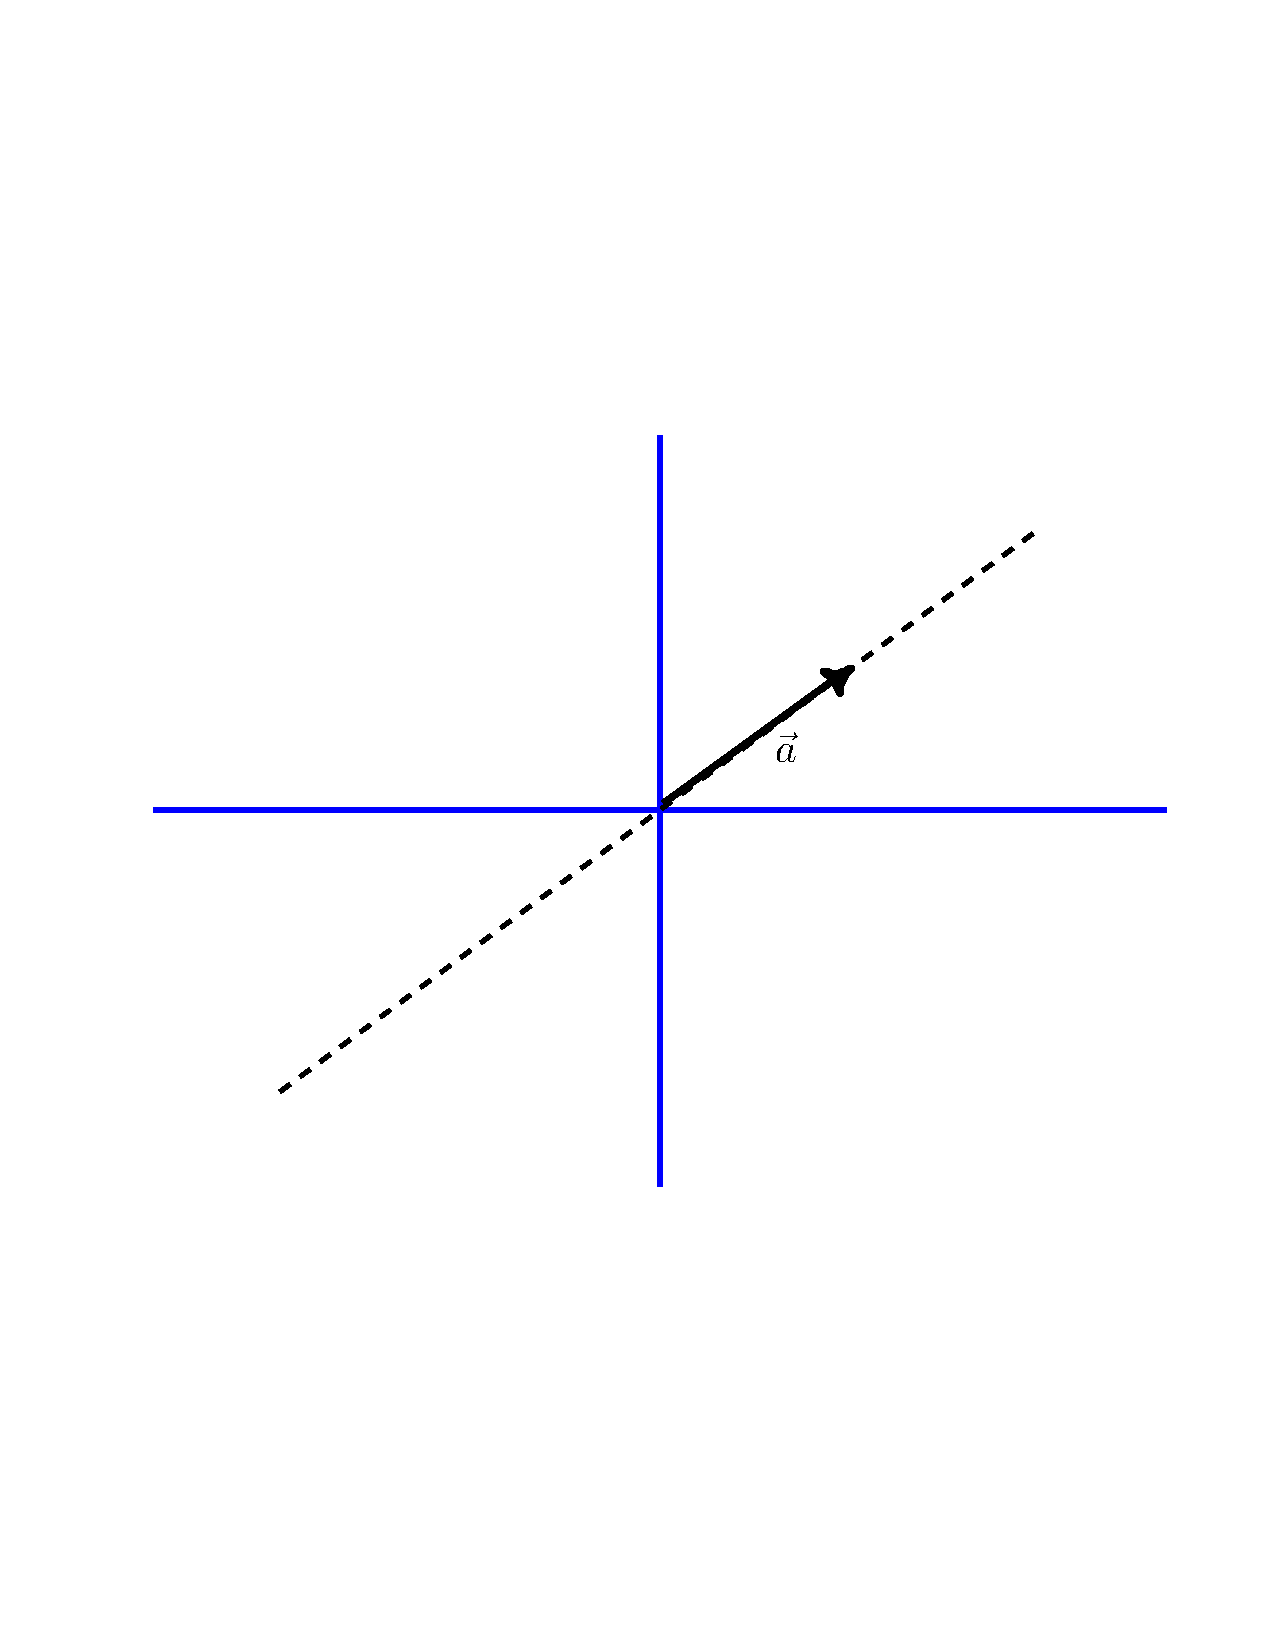
\includegraphics[height=3in]{2_2009_a1_3}}
\caption{Figure for Example \ref{2009_a1_3}. \label{ch2exnew1}}
\end{figure}

\subsection{Co-ordinates}

In order to do calculations with vectors, we have to introduce
co-ordinate axes.  Once we have chosen in what directions the
co-ordinate axes will lie, we can specify a vector by giving its
components in the co-ordinate directions.

\begin{figure}
\centerline{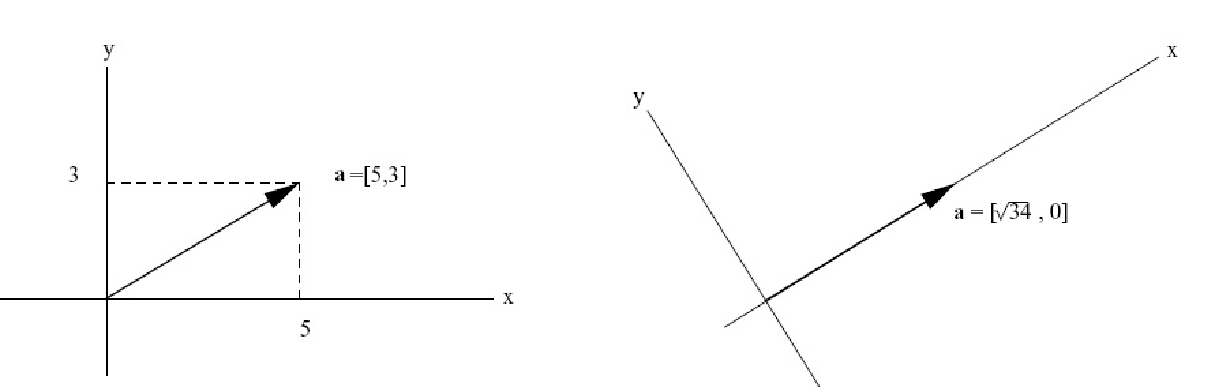
\includegraphics[height=2in]{2_coords}}
\caption{Two choices of co-ordinate axes. \label{fig_coords}}
\end{figure}

In the Figure~\ref{fig_coords} 
we see two choices of $x$ and $y$ axes. For the first
choice of axes, the vector $\aa$ has co-ordinates $[5,3]$ and for the
second choice of axes the co-ordinates are $[\sqrt{34},0]$. In a given
problem, it makes sense to choose the axes so that at least some of
the vectors have a simple representation. For example, in analyzing
the forces acting on a pendulum, we would either choose the $y$ axis
either to be vertical, or to lie along the shaft of the pendulum.

We can choose to write the co-ordinates of a vector in a row, as
above, or in a column, like
\[
\left[ \begin{array}{c} 
5 \\ 3 \end{array}
\right]
\]
Later on, we will almost always write vectors as columns. But in this
chapter we will write vectors as rows. Writing vectors as rows saves
space on the page but we will learn later how to write vectors in row
form even when we want them to be column vectors for other reasons. 
{\bf Note:} When writing vector coordinates by hand or in this text, either 
square or round brackets can be used. However, when using MATLAB, 
vectors must be created with square brackets (round brackets are used 
for other purposes). Other packages such as the online homework system, 
WeBWorK, may require different syntax. 

A convenient way to choose the co-ordinate axes is to specify unit
vectors (that is, vectors of length one) that lie along each of the
axes. These vectors are called standard basis vectors and are denoted
${\bf i}$ and ${\bf j}$ (in two dimensions) and ${\bf i}$, ${\bf j}$
and ${\bf k}$ (in three dimensions). These vectors are shown in 
Figure~\ref{fig_unitvecs}. Sometimes they are also denoted
${\bf e}_1$ and ${\bf e}_2$ or $\hat{\imath}$ and $\hat{\jmath}$ 
(in two dimensions) and ${\bf e}_1$, 
${\bf e}_2$ and ${\bf e}_3$ or $\hat{\imath}$, $\hat{\jmath}$ and $\hat{k}$ (in three dimensions). 
Different application areas have different conventions. 

\begin{figure}
\centerline{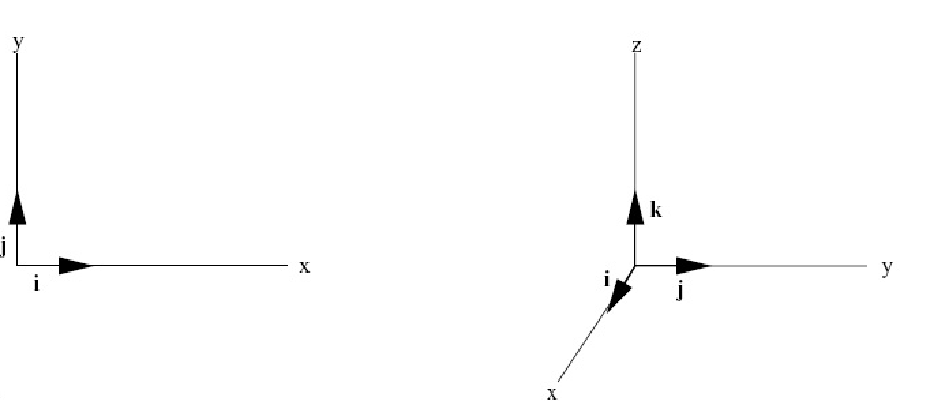
\includegraphics[height=2in]{2_unitvecs}}
\caption{Unit vectors in 2D (left) and 3D (right). \label{fig_unitvecs}}
\end{figure}

The unit vectors have co-ordinates 
\begin{eqnarray*}
{\bf i} &=& {\bf e}_1=[1,0] \\
{\bf j} &=& {\bf e}_2=[0,1] 
\end{eqnarray*}
in two dimensions, and
\begin{eqnarray*}
{\bf i}&=&{\bf e}_1=[1,0,0] \\
{\bf j}&=&{\bf e}_2=[0,1,0] \\
{\bf k}&=&{\bf e}_3=[0,0,1]
\end{eqnarray*}
in three dimensions.

Often, we make no distinction between a vector and its co-ordinate
representation. In other words, we regard the co-ordinate axes as
being fixed once and for all. Then a vector in two dimensions is
simply a list of two numbers (the components) $[a_1,a_2]$, and a
vector in three dimensions is a list of three numbers
$[a_1,a_2,a_3]$. Vectors in higher dimensions are now easy to
define. A vector in $n$ dimensions is a list of $n$ numbers
$[a_1,a_2,\ldots,a_n]$.

When a vector is multiplied by a number, each component is scaled by
the same amount. Thus if $\aa = [a_1,a_2]$, then
\begin{eqnarray*}
s\aa &=& s[a_1,a_2] \\
&=& [sa_1,sa_2]
\end{eqnarray*}

Similarly, when two vectors are added, their co-ordinates are added
component-wise. So if $\aa = [a_1,a_2]$ and $\bb=[b_1,b_2]$, then
\begin{eqnarray*}
\aa+\bb&=&[a_1,a_2]+[b_1,b_2]\\
&=&[a_1+b_1,a_2+b_2]
\end{eqnarray*}
This is shown in Figure~\ref{fig_coordadd}. 

\begin{figure}
\centerline{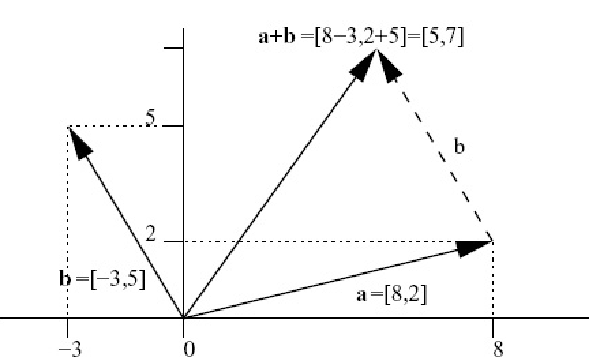
\includegraphics[height=2in]{2_coordadd}}
\caption{Adding vector co-ordinates. \label{fig_coordadd}}
\end{figure}

The analogous formulae hold in three (and higher dimensions). If 
$\aa=[a_1,a_2,\ldots,a_n]$ and $\bb = [b_1,b_2,\ldots,b_n]$, then
\begin{eqnarray*}
s\aa &=& s[a_1,a_2,\ldots,a_n]\\
&=&[sa_1,sa_2,\ldots,sa_n]\\
\aa+\bb&=&[a_1,a_2,\ldots,a_n]+[b_1,b_2,\ldots,b_n]\\
&=&[a_1+b_1,a_2+b_2,\ldots,a_n+b_n]
\end{eqnarray*}

\begin{example}
\label{2008_a1_1}
Sketch axes $x_1$-$x_2$. Add the vectors (1,1) and (2,-1) to
your sketch. Draw these vectors with base point at the origin. Now add
the vector (1,-2) to your sketch, starting at the base point
(1,1). That is, draw the vector with components 1 to the right and 2
down starting at (1,1). {\bf Note:}\ your sketch should show
graphically that (1,1)+(1,-2)=(2,-1). {\rm See Figure~\ref{ch2exnew2}.}
\end{example}

\begin{figure}[htb]
\centerline{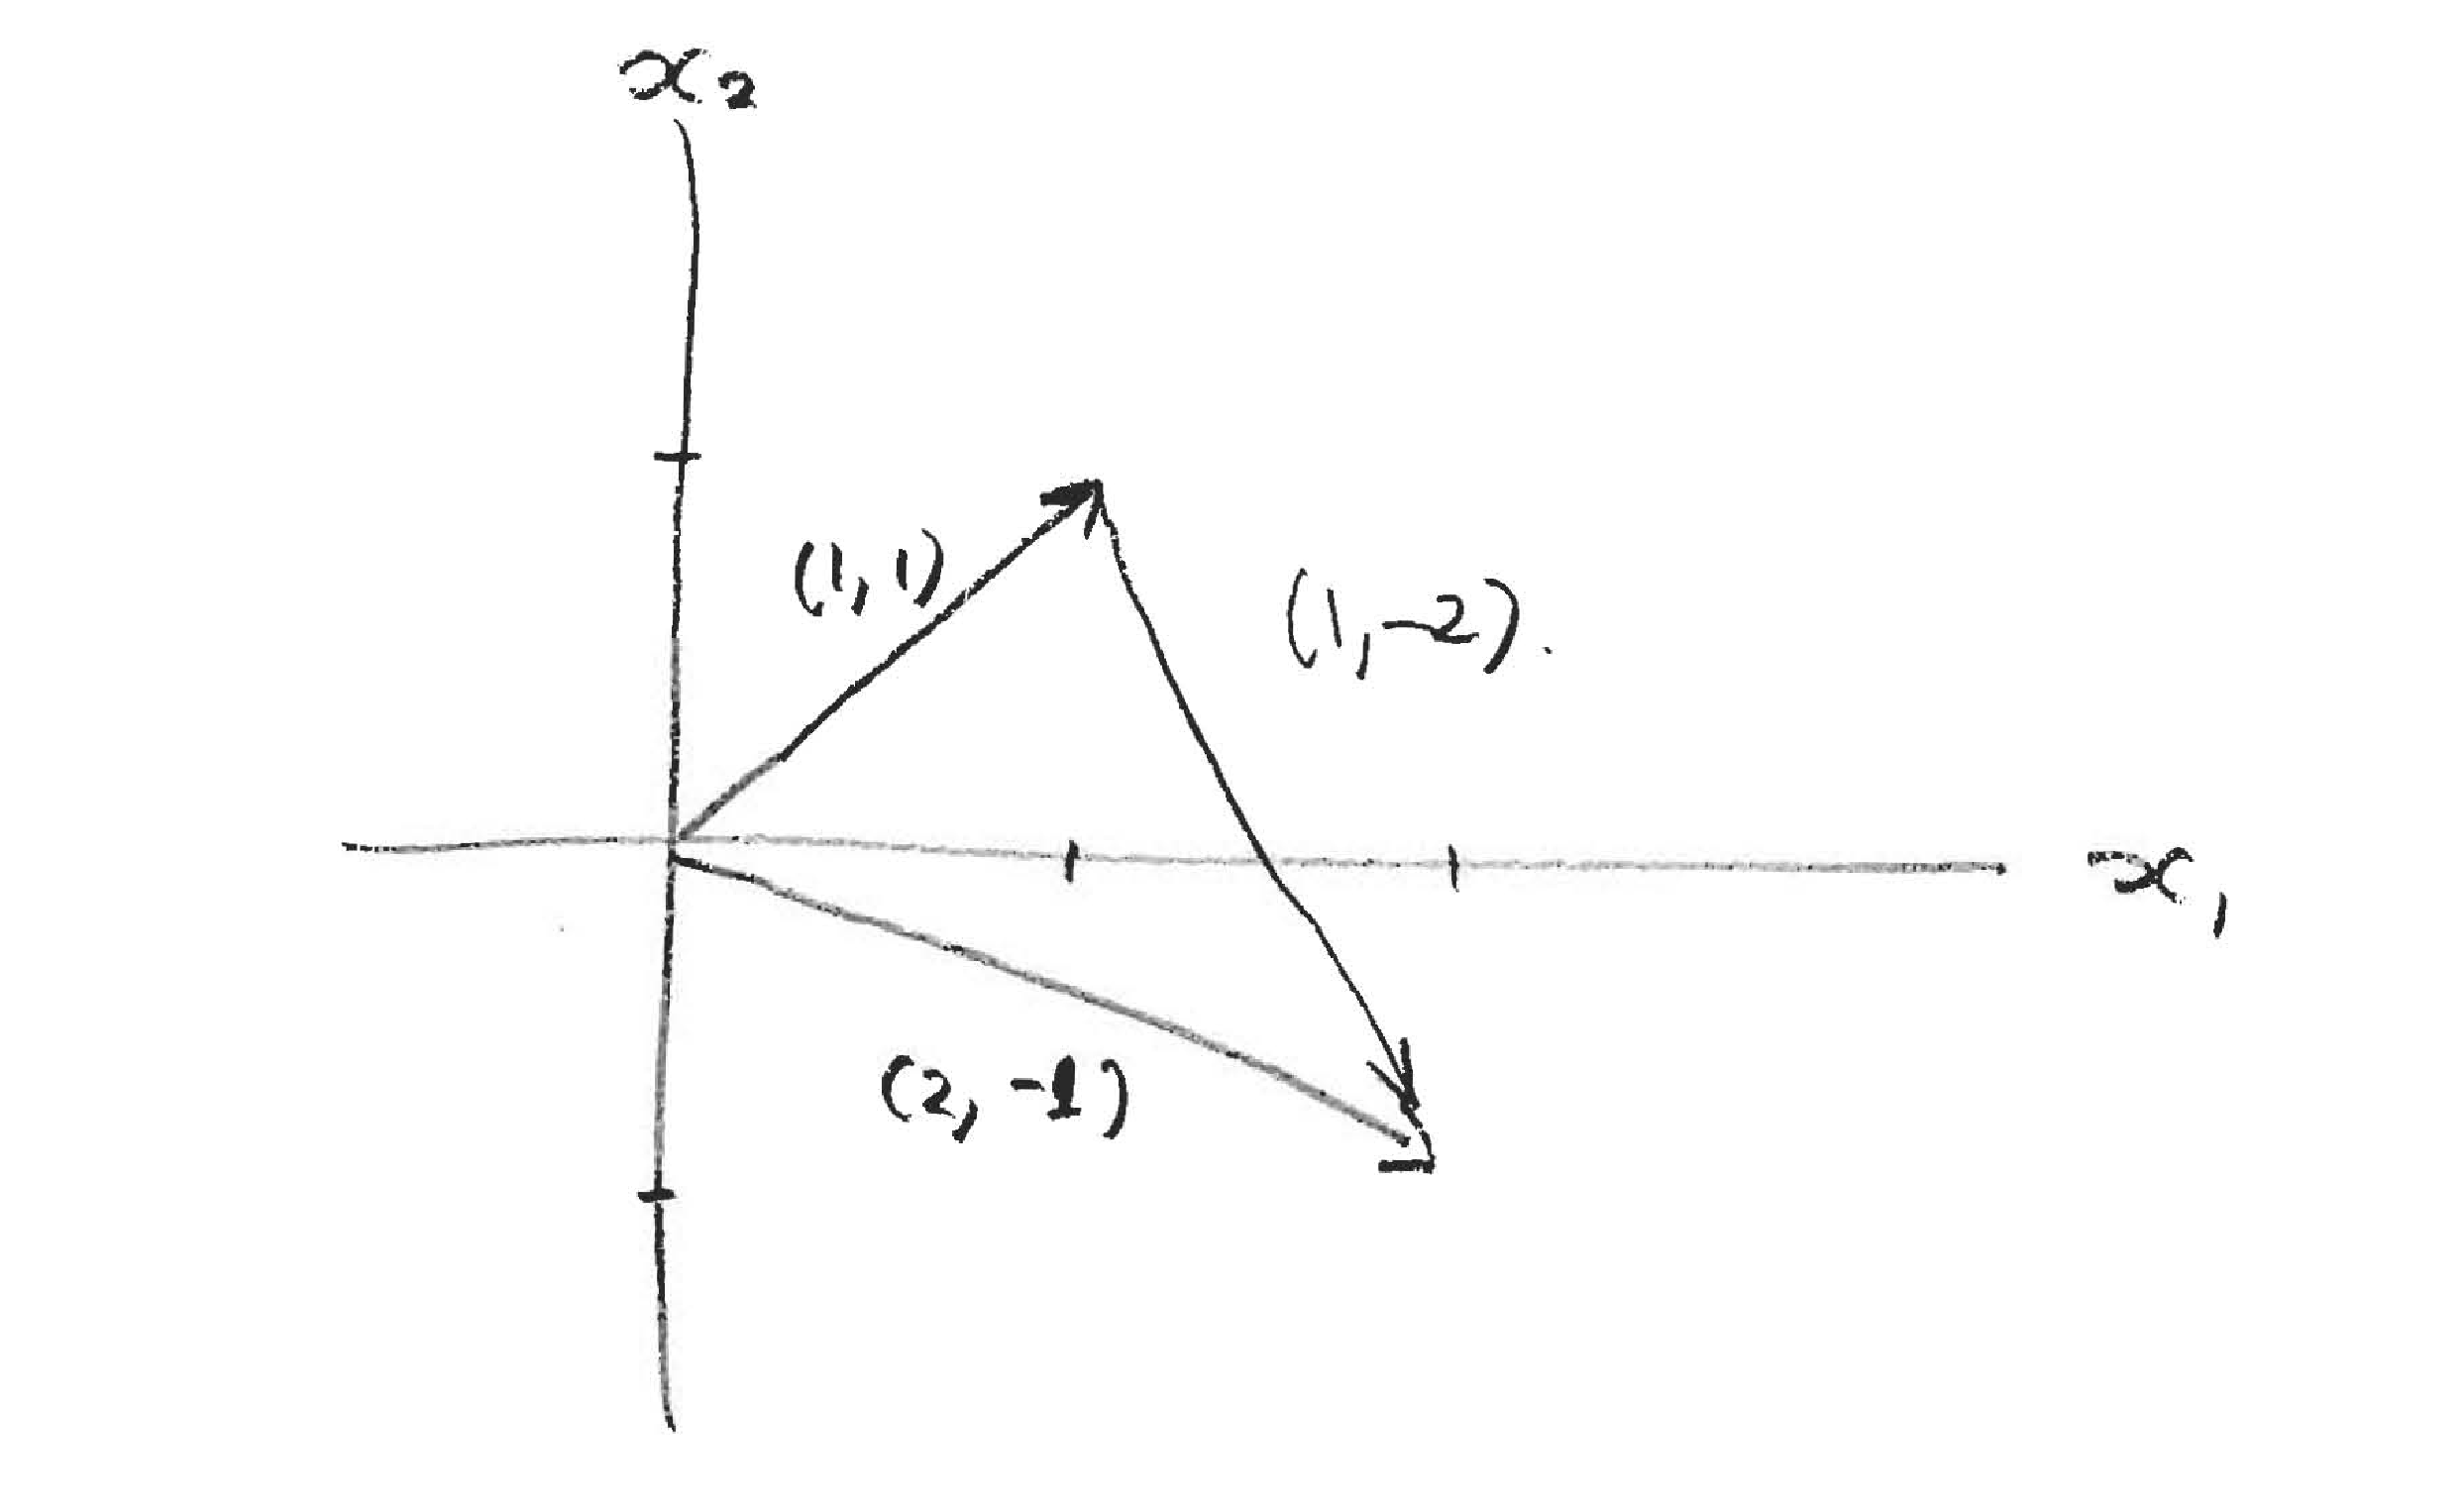
\includegraphics[height=1.5in]{2_newfig1}}
\caption{Figure for example \ref{2008_a1_1} \label{ch2exnew2}}
\end{figure}

\subsection{Properties of vector addition and scalar multiplication}

Let $\zv$ denote the zero vector. This is the vector all of whose
components are zero. The following properties are intuitive and easy
to verify.

\begin{enumerate}
\item $\aa+\bb=\bb+\aa$	
\item $\aa+(\bb+\cc)=(\aa+\bb)+\cc$
\item $\aa+\zv=\aa$
\item $\aa+(-\aa)= \zv$
\item $s(\aa+\bb)=(s\aa+s\bb)$
\item $(s+t)\aa=s\aa+t\aa$
\item $(st)\aa=s(t\aa)$	
\item $1\aa=\aa$
\end{enumerate}

They follow from similar properties which hold for numbers. For
example, for numbers $a_1$ and $b_1$ we know that $a_1+b_1 =
b_1+a_1$. Thus
\begin{eqnarray*}
\aa + \bb & = & [a_1,a_2]+[b_1,b_2] \\
& = & [a_1+b_1,a_2+b_2] = [b_1+a_1,b_2+a_2] \\
& = & [b_1,b_2]+[a_1,a_2] = \bb+ \aa, \\
\end{eqnarray*}
so property 1 holds.  Convince yourself that the rest of these
properties are true. (What is the vector $-\aa$?). It might seem like
a waste of time fussing over obvious properties such as
these. However, we will see when we come to the cross product and
matrix product, that sometimes such ``obvious'' properties turn out to
be false! It is important to know what the allowable operations for vectors 
(and matrices which we will see in later chapters) are since we will be doing 
algebra to solve matrix and vector equations. We will take special care to 
highlight the operations that have different properties from the scalar case.  

\subsection{MATLAB: basic scalar and vector operations}

There are MATLAB computer labs that accompany this course at UBC. You will be given 
an account on the Mathematics Department undergraduate network and instructions 
on how to access the computers in the labs and start the MATLAB application. 
A freely available google application, Octave, can execute all of the commands in the course 
with the same syntax. 
In the command window at the prompt {\tt >>} (MATLAB) or $\rhd$ (Octave), 
you can type MATLAB commands directly. Some basic commands are given below 
\begin{description}
\item[{\bf assignment:}] Scalar and vector variables can be assigned 
using the ``=" operator. For example 
\begin{verbatim}
a = 2 
\end{verbatim}
followed by {\tt <enter>} 
assigns the scalar value of 2 to the variable {\tt a}. The result 
of the command is printed out although this can be suppressed by using a 
colon at the end of the command:
\begin{verbatim}
a = 2;
\end{verbatim}
Here {\tt a} is still assigned the value of 2 but no output is generated. 
Vector variables are assigned with the following notation:
\begin{verbatim}
b = [1 2];
\end{verbatim}
Note that {\tt b = [1, 2]} has the same meaning in MATLAB, i.e., numbers separated by a comma or a space imply row vectors. For column vectors, the entries have to be separated by semicolons:
\begin{verbatim}
b1 = [2; 3];
\end{verbatim}

Note also that there are no special distinctions between the names of scalar and
vector variables. 
\item[{\bf addition:}] Both scalar and vector addition can be done with 
the ``+" operator. Keeping the values of scalar {\tt a} and vector {\tt b} 
above, we enter the commands
\begin{verbatim}
a2 = 5;
b2 = [2 9];
a+a2
c = b+b2;
\end{verbatim}
The first two lines above assign a new scalar and vector. The third line 
prints out the answer 7 (2+5). The last line assigns the resulting vector 
[3 11] ([1 2] + [2 9]) to the new vector {\tt c} but prints nothing. 
\item[{\bf scalar multiplication}] Scalar multiplication (of vectors and 
other scalars) is implemented using the ``*" command. Using the variables 
defined above,
\begin{verbatim}
a*a2
a*b 
\end{verbatim}
would result in 10 (2 times 5) and [2 4] (2 times [1 2]). The ``*" command 
also implements matrix-vector and matrix-matrix multiplication discussed 
later in the course. Vector-vector multiplication (dot products and 
cross products) are implemented using different commands as discussed in the 
next section. 
\item[{\bf other commands:}] There are many useful functions built 
in to MATLAB such as {\tt sqrt} (square root), {\tt cos} (cosine, taking 
an argument in radians), {\tt acos} (inverse cosine, giving an result 
in radians) and many more. They are called as follows
\begin{verbatim}
sqrt(2)
\end{verbatim}
which will return $\sqrt{2}$ to 4 decimal places. Type {\tt help} followed
by a command name gives you a description of that command. Try 
typing {\tt help atan2} since {\tt atan2} is a pretty useful function. 
These MATLAB functions can take vector arguments, they act on each 
entry of the vector. For example 
\begin{verbatim}
sqrt([1 4])
\end{verbatim}
will produce the vector [1 2]. 
\end{description}

\subsection{Problems} 

\begin{problem}
  \label{2009_a1_1}
Sketch axes $x_1$-$x_2$. Add the vectors (2,2) and (1,-1) to
your sketch. Draw these vectors with base point at the origin. Now add
the vector (1,-1) to your sketch, starting at the base point
(2,2). That is, draw the vector with components 1 to the right and 1
down starting at (2,2). {\bf Note:}\ your sketch should show
graphically that (2,2)+(1,-1)=(3,1).
\end{problem}

\begin{problem}
\label{op1_1}
Let $\aa$, $\bb$ and $\cc$ be fixed non-zero vectors. Describe and
sketch the following sets of points in two and three dimensions:
\begin{enumerate}
\renewcommand{\labelenumi}{(\roman{enumi})}
\item $\{s\aa : s\in\RR\}$ (i.e., the set of all scalar multiples of
$\aa$)\par
\item $\{s\aa : s>0\}$ (i.e., the set of all positive scalar multiples
of $\aa$)\par
\item $\{\bb + s\aa : s\in\RR\}$\par
\item $\{s\aa + t\bb : s,t\in\RR\}$\par
\item $\{\cc + s\aa + t\bb : s,t\in\RR\}$\par
\end{enumerate}
\end{problem}

\begin{problem}
\label{op1_2}
Describe the vectors $\aa - \bb$ and $\bb - \aa$.
\end{problem}

\begin{problem}
\label{op1_3}
Find an expression for the midpoint between $\aa$ and $\bb$. Find an expression
for a point one third of the way between $\aa$ and $\bb$.
\end{problem}

\begin{problem}
\label{op1_4}
Find an expression for the line segment joining $\aa$ and $\bb$.
\end{problem}

\section{Geometrical Aspects of Vectors}

\subsection{Length of a vector}

It follows from the Pythagorean formula that the length $\|\aa\|$ of
$\aa=[a_1,a_2]$ satisfies $\|\aa\|^2=a_1^2+a_2^2$. This is shown in 
Figure~\ref{fig_pyth}.

\begin{figure}
\centerline{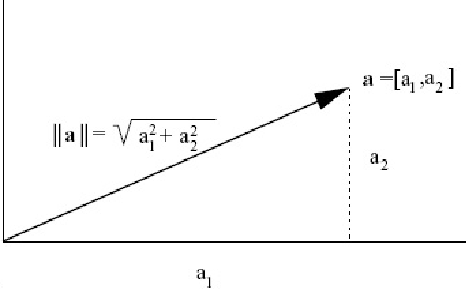
\includegraphics[height=2in]{2_pyth}}
\caption{Pythagorean Formula. \label{fig_pyth}}
\end{figure}

Thus
\[
\|\aa\|= \sqrt{a_1^2+a_2^2}.
\]
Similarly, for a vector $\aa=[a_1,a_2,a_3]$ in three dimensions,
\[
\|\aa\|= \sqrt{a_1^2+a_2^2+a_3^2}.
\]
The distance between two vectors $\aa$ and $\bb$ is the length of the
difference $\bb-\aa$.

\subsection{The dot product}

The dot product of two vectors is defined in both two and three
dimensions (actually in any dimension). The result is a number. Two
main uses of the dot product are testing for orthogonality and
computing projections.

The dot product of $\aa=[a_1,a_2]$ and $\bb=[b_1,b_2]$ is given by
\[
\aa\cdot\bb = a_1b_1 + a_2b_2.
\]
Similarly, the dot product of $\aa=[a_1,a_2,a_3]$ and
$\bb=[b_1,b_2,b_3]$ is given by
\[
\aa\cdot\bb = a_1b_1 + a_2b_2 + a_3b_3.
\]
The properties of the dot product are as follows:
\begin{description}
\item[0.] If $\aa$ and $\bb$ are vectors, then $\aa\cdot\bb$ is a number.
\item[1.] $\aa\cdot\aa = \|a\|^2$.
\item[2.] $\aa\cdot\bb = \bb\cdot\aa$.
\item[3.] $\aa\cdot(\bb+\cc) = \aa\cdot\bb + \aa\cdot\cc$.
\item[4.] $s(\aa\cdot\bb) = (s\aa)\cdot\bb$.
\item[5.] $\zv\cdot\aa=0$.
\item[6.] $\aa\cdot\bb = \|\aa\|\|\bb\|\cos(\theta)$, where $\theta$
is angle between $\aa$ and $\bb$.  
\item[7.] $\aa\cdot\bb = 0$ $\iff$ $\aa=\zv$ or $\bb=\zv$ or $\aa$ and
$\bb$ are orthogonal (i.e,. perpendicular).
\end{description}
Properties 0 to 5 are easy consequences of the definitions. 
For example, to
verify property 5 we write
\[
\zv\cdot\aa = [0,0,0]\cdot[a_1,a_2,a_3]= 0a_1+0a_2+0a_3=0.
\]

Property 6 is the most important property and is often taken as the
definition of the angle $\theta$ between vectors $\bf a$ and $\bf b$.  
Notice that our definition is given in terms of the
components of the vectors, which depend on how we chose the
co-ordinate axes. It is not at all clear that if we change the
co-ordinate axis, and hence the co-ordinates of the vectors, that we
will get the same answer for the dot product. However, property 6 says
that the dot product only depends on the lengths of the vectors and
the angle between them. These quantities are independent of how
co-ordinate axes are chosen, and hence so is the dot product.

To show that property 6 holds we compute $\|\aa-\bb\|^2$ in two
different ways.  First of all, using properties 1 to 5, we have
\begin{eqnarray}
\nonumber
\|\aa-\bb\|^2 & = & (\aa-\bb)\cdot(\aa-\bb) \\
 \nonumber
 & = & \aa\cdot\aa - \aa\cdot\bb - \bb\cdot\aa + \bb\cdot\bb \\
\label{ch2_theta1}
 & = & \|\aa\|^2 + \|\bb\|^2 - 2 \aa\cdot\bb
\end{eqnarray}
(Which properties were used in each step?) Next we compute
$\|\aa-\bb\|$ as depicted in Figure~\ref{fig_cos2} (left). 

\begin{figure}
\centerline{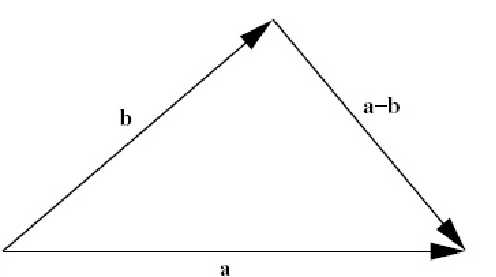
\includegraphics[height=1.5in]{2_cos1}
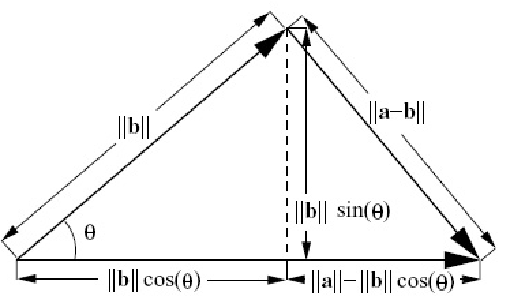
\includegraphics[height=1.5in]{2_cos2}}
\caption{The vectors $\aa$, $\bb$ and $\aa-\bb$ (left) 
Lengths of Segments (right). \label{fig_cos2}}
\end{figure}

We mark the lengths of each of the line segments in Figure~\ref{fig_cos2}
(right). 
Using Pythagoras' theorem for the right angled triangle on the right
of this diagram, we see that
\[
\|\aa-\bb\|^2 = (\|\aa\|-\|\bb\|\cos(\theta))^2 + \|\bb\|^2\sin^2(\theta).
\]
Thus, using $\cos^2(\theta)+\sin^2(\theta)=1$,
\begin{eqnarray}
\nonumber
\|\aa-\bb\|^2 & = & \|\aa\|^2+\|\bb\|^2\cos^2(\theta) -
2\|\aa\|\|\bb\|\cos(\theta) + \|\bb\|^2\sin^2(\theta) \\
\label{ch2_theta2}
 & = & \|\aa\|^2+\|\bb\|^2 - 2\|\aa\|\|\bb\|\cos(\theta)
\end{eqnarray}
Actually, this is just the cosine law applied to the triangle in Figure~\ref{fig_cos2}
and you may have been able to write (\ref{ch2_theta2}) directly. 
Now we equate the two expressions (\ref{ch2_theta1}, \ref{ch2_theta2}) 
for $\|\aa-\bb\|^2$. This gives
\[
\|\aa\|^2 + \|\bb\|^2 - 2 \aa\cdot\bb = \|\aa\|^2+\|\bb\|^2 -
2\|\aa\|\|\bb\|\cos(\theta)
\]
Subtracting $\|\aa\|^2 + \|\bb\|^2$ from both sides and dividing by
$-2$ now yields
\[
\aa\cdot\bb=\|\aa\|\|\bb\|\cos(\theta).
\]
This proves property 6.

Property 7 now follows directly from 6. If $\aa\cdot\bb = 0$ then
$\|\aa\|\|\bb\|\cos(\theta)=0$ so either $\|\aa\|=0$, in which case
$\aa=\zv$, or $\|\bb\|=0$, in which case $\bb=\zv$, or
$\cos(\theta)=0$, which implies that $\theta = \pi/2$ (since $\theta$
lies between $0$ and $\pi$).  This implies $\aa$ and $\bb$ are
orthogonal.

Property 6 can be used to compute the angle between two vectors as shown in the example below.  
\begin{example}
What is the angle between the vectors whose tails lie at the
centre of a cube and whose heads lie on adjacent vertices?  {\rm To compute
this take a cube of side length $2$ and centre it at the origin, so
that the vertices lie at the points $[\pm 1, \pm 1, \pm1]$.  Then we
must find the angle between $\aa=[1, 1, 1]$ and $\bb=[-1, 1, 1]$.
Since
\[
\aa\cdot\bb = -1 + 1 + 1 = 1 =
\|\aa\|\|\bb\|\cos(\theta)=\sqrt{3}\sqrt{3}\cos(\theta)
\]
we obtain
\[
\theta = \arccos(1/3) \sim 1.231 \quad (\sim 70.5^\circ)
\]}
\end{example}

\begin{example}
For what value (or values) of $s$ is the vector $[1,1,s]$ perpendicular to  $[1,5,3]$? 
{\rm The dot product of the two vectors must be zero for them to be orthogonal. We compute 
\[
[1,1,s] \cdot [1,5,3] = 1+5+3s 
\]
so $6+3s=0$ for orthogonality, $s=-2$.} 
\end{example} 

Here is an example to review the basic operations on vectors we know so far.
\begin{example}
% \label{2008_a1_2}
Consider the vectors ${\bf a} = (2,3)$ and ${\bf b} =
(1,-3)$ in $\mathbb{R}^2$. Compute the following:
{\begin{enumerate}
\renewcommand{\labelenumi}{(\alph{enumi})}
\item ${\bf a} + {\bf b}$
\item $3 {\bf a}$
\item $2{\bf a} + 4{\bf b}$
\item ${\bf a} \cdot {\bf b}$
\item $\| {\bf b} \|$
\end{enumerate}}
{\rm Solutions:
\begin{enumerate}
\renewcommand{\labelenumi}{(\alph{enumi})}
\item $\aa + \bb = (2,3)+(1,-3) = (3,0)$
\item $3 \aa = 3 (2,3) = (6,9)$
\item $2\aa + 4\bb = 2(2,3) + 4(-1,3) = (4,6)+(4,-12) = (8,-6)$
\item $\aa \cdot \bb = (2,3) \cdot (1,-3) = 2-9 = -7$.
\item $\| \bb \| = \sqrt{1^2 + (-3)^2} = \sqrt{10}$.
\end{enumerate}}
\end{example}

\subsection{Projections and Unit Vectors}

Suppose $\aa$ and $\bb$ are two vectors. The projection of $\aa$ in
the direction of $\bb$, denoted ${\rm proj}_\bb\aa$, is the vector in
the direction of $\bb$ whose length is determined by drawing a line
perpendicular to $\bb$ that goes through $\aa$.  In other words, the
length of ${\rm proj}_\bb\aa$ is the component of $\aa$ in the
direction of $\bb$. This is shown in Figure~\ref{fig_proj}

\begin{figure}
\centerline{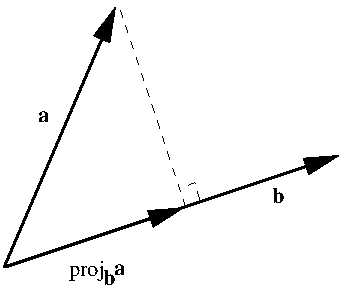
\includegraphics[height=1.5in]{2_proj}}
\caption{Projection. \label{fig_proj}}
\end{figure}

To compute ${\rm proj}_\bb\aa$, we first note that it is a multiple of
$\bb$.  Thus ${\rm proj}_\bb\aa = s\bb$ for some number $s$. To
compute $s$, we use the fact that the vector ${\rm proj}_\bb\aa - \aa$
(along the dotted line in the diagram) is orthogonal to $\bb$. Thus
$({\rm proj}_\bb\aa - \aa)\cdot\bb = 0$, or $(s\bb-\aa)\cdot\bb=0$, or
$s = \aa\cdot\bb / \bb\cdot\bb = \aa\cdot\bb / \|\bb\|^2$. Thus
\begin{equation}
\label{eq:projection}
{\rm proj}_\bb\aa = {{\aa\cdot\bb}\over{\|\bb\|^2}}\bb.
\end{equation}
If $\bb$ is a unit vector (i.e., $\|\bb\|=1$, length 1) this expression is even
simpler. We will use the notation $\hat{b}$ to denote unit vectors. In this case
\[
{\rm proj}_{\hat{b}} \aa = (\aa\cdot\hat{b})\,\hat{b}.
\]

It is easy to find a unit vector $\hat{b}$ that points in the same direction as any nonzero 
vector $\bb$, simply compute 
\[
\hat{b} = \frac{1}{\| \bb \|} \bb.
\]
Since $\hat{b}$ is a (positive) scalar multiple of $\bb$ in the above formula, it clearly points in the
same direction as $\bb$. A straight forward calculation shows that $\hat{b}$ has unit length 
(try it!). 

\begin{example}
Find the unit vector $\hat{b}$ that points in the same direction as $\bb = [1, 2]$.
{\rm We compute 
\[
\| \bb \| = \sqrt{1^2 + 2^2} = \sqrt{5}
\]
and then 
\[
\hat{b} = \frac{1}{\sqrt{5}} [1,2] = [1/\sqrt{5}, 2/\sqrt{5}]. 
\]} 
\end{example}

Projections are useful for computing the components of a vector in
various directions. An easy example is given be the co-ordinates of a
vector. These are simply the components of a vector in the direction
of the standard basis vectors. So in two dimensions
\begin{eqnarray*}
a_1 & = & \aa\cdot{\bf i} = [a_1,a_2]\cdot[1,0] \\
a_2 & = & \aa\cdot{\bf j} = [a_1,a_2]\cdot[0,1]
\end{eqnarray*}

\begin{example}
Let $\aa = [1,0,2]$ and $\bb = [0, 5, 2]$. Compute 
$ \mbox{proj}_{\bf b} {\bf a}$ (the projection of $\bf a$ in the
direction of $\bf b$).
{\rm We use (\ref{eq:projection}) and first compute 
\[
\| \bb \|^2 = 5^2 + 2^2 = 29 \mbox{\ \ \ and $\aa \cdot \bb = 4$}, 
\]
then 
\[
\mbox{proj}_{\bf b} {\bf a} = \frac{4}{29} [0, 5, 2] = [0, 20/29, 8/29].
\]}
\end{example}

\subsection{MATLAB: {\tt norm} and {\tt dot}  commands}

MATLAB has built-in functions that implement most of the mathematical 
operations introduced this course. For example, the commands 
\begin{description}
\item[{\tt norm(a)}] returns the length (norm) of the vector {\tt a}. 
\item[{\tt dot(a,b)}] returns the dot product of the vectors 
{\tt a} and {\tt b} (if the vectors do not have the same length, an 
error results as you would expect). 
\end{description}
Using these commands and scalar multiplication of vectors, a projection 
of {\tt a} onto the direction {\tt b} can be implemented:
\begin{verbatim}
(dot(a,b)/norm(b)^2))*b
\end{verbatim}
where {\tt /} denotes division (of scalar quantities in this case) and 
{\tt \^\ p} gives the p'th power of a quantity. 

\subsection{Problems}

\begin{problem}
  \label{2009_a1_2}
Consider the vectors ${\bf a} = (1,2)$ and ${\bf b} =
(1,-2)$ in $\mathbb{R}^2$ (the set of vectors with 2 components).
Compute the following:
\begin{enumerate}
\item ${\bf a} + {\bf b}$
\item $2 {\bf a}$
\item ${\bf a} - {\bf b}$
\item ${\bf a} \cdot {\bf b}$
\item $\| {\bf b} \|$
\end{enumerate}
\end{problem}

\begin{problem}
\label{2008_a1_3}
A circle in the $x_1$-$x_2$ plane has centre at (2,5). A given
point on its circumference is (3,3). Write an equation that describes
all the points $(x_1,x_2)$ on the circle. 
\end{problem}

\begin{problem}
\label{op1_5}
Find the equation of a sphere centred at $\aa=[a_1,a_2,a_3]$ with
radius $r$.  (Hint: the sphere is the set of points
$\xx=[x_1,x_2,x_3]$ whose distance from $\aa$ is $r$
\end{problem}

\begin{problem}
\label{op1_6}
Find the equation of a sphere if one of its diameters has endpoints
$[2,1,4]$ and $[4,3,10]$
\end{problem}

\begin{problem}
\label{op1_7}
Compute the dot product of the vectors $\aa$ and $\bb$ and find the angle
between them.
{\begin{enumerate}
\renewcommand{\labelenumi}{(\roman{enumi})}
\item $\aa=[1,2]$, $\bb=[-2,3]$
\item $\aa=[-1,2]$, $\bb=[1,1]$
\item $\aa=[1,1]$, $\bb=[2,2]$
\item $\aa=[1,2,1]$, $\bb=[-1,1,1]$
\item $\aa=[-1,2,3]$, $\bb=[3,0,1]$
\end{enumerate}}
\end{problem}

\begin{problem}
\label{2009_a1_4}
Let ${\bf a} = (1,1,1)$ and ${\bf b} = (3,1,-2)$. Compute the
following:
\begin{enumerate}
\item The angle between ${\bf a}$ and ${\bf b}$.
\item $ \mbox{proj}_{\bf a} {\bf b}$ (the projection of $\bf b$ in the
direction of $\bf a$).
\end{enumerate}
\end{problem}

\begin{problem}
\label{2008_a1_5}
Let ${\bf a} = (1,4,0)$ and ${\bf b} = (2,-1,5)$. Compute the
following:
{\begin{enumerate}
\renewcommand{\labelenumi}{(\alph{enumi})}
\item The angle between ${\bf a}$ and ${\bf b}$.
\item $ \mbox{proj}_{\bf a} {\bf b}$ (the projection of $\bf b$ in the
direction of $\bf a$). 
\end{enumerate}}
\end{problem}

\begin{problem}
\label{op1_8}
For which value of $s$ is the vector $[1,2,s]$ orthogonal to
$[-1,1,1]$?
\end{problem}

\begin{problem}
\label{op1_9}
Does the triangle with vertices $[1,2,3]$, $[4,0,5]$ and $[3,4,6]$
have a right angle? 
\end{problem}

\begin{problem}
\label{2009_a1_5}
Determine the values of $c_1$ and $c_2$ such that the vector
[$c_1$ 1 $c_2$] is a scalar multiple of [2 -2 3]. 
\end{problem}

\begin{problem}
\label{op1_10}
An air-plane with an approach speed of 70 knots is on approach to
runway 26 (i.e., pointing in the direction of 260 degrees). This 
is shown in Figure~\ref{fig_runway} (left). If the
wind is from 330 degrees at 10 knots, what heading should the pilot
maintain to stay lined up with the runway? What is the groundspeed of
the air-plane?
\end{problem}

\begin{figure}
\centerline{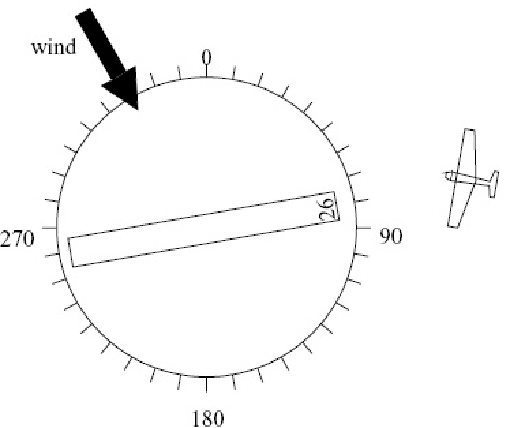
\includegraphics[height=1.5in]{2_runway}
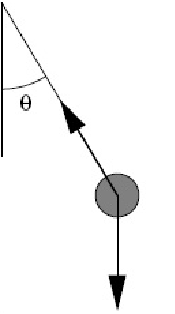
\includegraphics[height=1.5in]{2_pend2}}
\caption{Runway diagram for problem~\ref{op1_10} (left) and 
the pendulum of problem~\ref{op1_11} (right) \label{fig_runway}}
\end{figure}

\begin{problem}
\label{op1_11}
Suppose the angle of the pendulum shaft makes an angle of $\theta$
with the vertical direction as 
shown in Figure~\ref{fig_runway} (right). The force of gravity has
magnitude (length) equal to $mg$ and points downwards. The force along
the shaft of the pendulum acts to keep the shaft rigid, i.e., the
component of the total force along the shaft is zero. Write down the
co-ordinates of the two forces and the total force using two different
sets of co-ordinate axes --- one horizontal and vertical, and one
parallel to and orthogonal to the shaft of the pendulum.
\end{problem}


\begin{problem}
\label{matlab_op1_11}
(Matlab) In Matlab code, if one defines a vector $\aa=[a_1,a_2,\cdots,a_n]$, with the $a_i$'s being any numbers, the output of typing $\aa(j)$ would be $a_j$.

Suppose that you have a two element vector. How would you write a line of Matlab code to compute the norm of the vector, without using the {\tt norm} or {\tt dot} commands?
\end{problem}

\section{Determinants and the Cross Product}

\subsection{The determinant in two and three dimensions}
\label{s:trick} 

The determinant is a number that is associated with a square matrix,
that is, a square array of numbers.

In two dimensions it is defined by
\[
\det\left[\matrix{a_1&a_2\cr b_1&b_2\cr}\right]=a_1b_2-a_2b_1.
\]

\begin{example}
Find the determinant of 
\[
\left[\matrix{1 & 2 \cr 3 & 4 \cr}\right].
\]
{\rm Using the formula above, we have that the determinant is 
\[
1\times 4 - 2 \times 3 = -2. 
\]
}
\end{example}

\noindent The definition in three dimensions is
\begin{eqnarray*}
\det \left[ \begin{array}{ccc}
	a_1&a_2&a_3 \\
	b_1&b_2&b_3 \\
	c_1&c_2&c_3
	    \end{array}
\right]
 & = & a_1\det\left[\matrix{b_2&b_3\cr c_2&c_3\cr}\right]
       - a_2\det\left[\matrix{b_1&b_3\cr c_1&c_3\cr}\right]
+ a_3\det\left[\matrix{b_1&b_2\cr c_1&c_2\cr}\right] \\
 & = & a_1b_2c_3-a_1b_3c_2 + a_2b_3c_1-a_2b_1c_3 + a_3b_1c_2-a_3b_2c_1
\end{eqnarray*}

We want to determine the relationship between the determinant and the
vectors $\aa=[a_1,a_2]$ and $\bb = [b_1,b_2]$ (in two dimensions) and
$\aa=[a_1,a_2,a_3]$, $\bb = [b_1,b_2,b_3]$ and $\cc=[c_1,c_2,c_3]$ (in
three dimensions). We will do the two dimensional case now, but
postpone the three dimensional case until after we have discussed the
cross product.

\begin{example}
Find the determinant of 
\[
A = \left[ \begin{array}{ccc}
	1 & 1 & 0 \\
	4 & 2 & 2 \\
	1 & 0 & 3
	    \end{array}
\right].	    
\]
{\rm It is easiest to remember the formula using the first line in the equation above 
using the determinants of the corresponding $2 \times 2$ blocks of the matrix. 
\[
\det A = 1 (2 \times 3-0) -1 (4 \times 3 -2) + 0 = -4. 
\]
}
\end{example}

So let $\aa=[a_1,a_2]$ and $\bb = [b_1,b_2]$ be two vectors in
the plane. Define
\[
\aa^\perp = [-a_2,a_1].
\]
Notice that $\aa^\perp$ has the same length as $\aa$, and is
perpendicular to $\aa$, since
\[
\aa^\perp\cdot\aa = -a_2a_1 + a_1a_2 = 0.
\]
There are exactly two vectors with these properties. The vector
$\aa^\perp$ is the one that is obtained from $\aa$ by a counterclockwise
rotation of $\pi/2$ (i.e., $90^\circ$). To see this, notice that if
$\aa$ lies in the first quadrant (that is, $a_1>0$ and $a_2>0$) then
$\aa^\perp$ lies in the second quadrant, and so on. Later in the course
we will study rotations and this will be a special case.
Notice now that the determinant can be written as a dot product.
\[
\aa^\perp\cdot\bb = -a_2b_1+a_1b_2 = \det\left[\matrix{a_1&a_2\cr
b_1&b_2\cr}\right]
\]
We want to use the geometric formula for the dot product of $\aa^\perp$
and $\bb$. Let $\theta$ be the angle between $\aa$ and $\bb$ and
$\pi/2-\theta$ be the angle between $\aa^\perp$ and $\bb$, as shown in
Figure~\ref{fig_ppgram2}.

\begin{figure}
\centerline{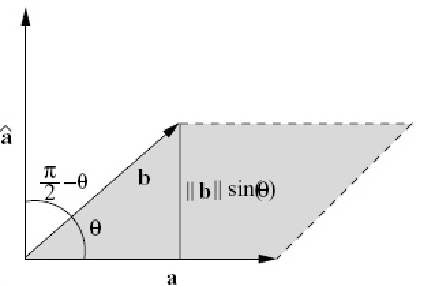
\includegraphics[height=2in]{2_ppgram2}}
\caption{The vector $a^\perp$ (labelled incorrectly in the figure as $\hat{a}$). \label{fig_ppgram2}}
\end{figure}

Using the geometric meaning of the dot product, we obtain
\begin{eqnarray*}
\det\left[\matrix{a_1&a_2\cr b_1&b_2\cr}\right]
 & = & \aa^\perp\cdot\bb \\
 & = & \|\aa^\perp\|\|\bb\|\cos(\pi/2-\theta) \\
 & = & \|\aa\|\|\bb\|\sin(\theta)
\end{eqnarray*}
We need to be a bit careful here.  When we were discussing the dot
product, we always assumed that the angle between two vectors was in
the range $0$ to $\pi$.  In fact, the geometric formula for the dot
product is not sensitive to how we measure the angle. Suppose that
instead of $\theta$ in the range $0$ to $\pi$ we use
$\theta_1=-\theta$ (measuring the angle ``backwards'') or
$\theta_2=2\pi-\theta$ (measuring the angle going the long way around
the circle). Since $\cos(\theta)=\cos(-\theta)=\cos(2\pi-\theta)$ we
have
\[ \cc\cdot\dd=\|\cc\|\|\dd\|\cos(\theta)=\|\cc\|\|\dd\|\cos(\theta_1)
=\|\cc\|\|\dd\|\cos(\theta_2).
\]
In other words, the geometric formula for the dot product still is
true.

In the diagram above, we want to let the angle $\theta$ between $\aa$
and $\bb$ range between $-\pi$ and $\pi$.  In this case the angle
$\pi/2-\theta$ between $\aa^\perp$ and $\bb$ is sometimes not in the
range between $0$ or $2\pi$. But if this happens, then it is still the
angle between $\aa^\perp$ and $\bb$, just ``backwards'' or ``the long
way around.'' Thus the geometric formula above still is correct.

Values of $\theta$ between $0$ and $\pi$ correspond to the situation
where the direction of $\bb$ is obtained from the direction of $\aa$
by a counterclockwise rotation of less than $\pi$. This is the case in
the diagram. On the other hand, $\theta$ between $-\pi$ and $0$
corresponds to the case where a clockwise rotation of less than $\pi$
is needed to get from the direction of $\aa$ to the direction of
$\bb$.

The quantity $\sin(\theta)$ can be positive or negative, depending on
the orientations of $\aa$ and $\bb$, but in any case the positive
quantity $\|\bb\||\sin(\theta)|$ is the height of the parallelogram
spanned by $\aa$ and $\bb$ if we take $\aa$ to be the base. In this
case, the length of the base is $\|\aa\|$. Recall that the area of a
parallelogram is the length of the base times the height. Thus
\[
\left|\det\left[\matrix{a_1&a_2\cr b_1&b_2\cr}\right]\right|
=\hbox{Area of parallelogram spanned by $\aa$ and $\bb$}
\]
The determinant is positive if $\sin(\theta)$ is positive, that is, if
$\theta$ is positive. This is the case if the direction of $\bb$ is
obtained by a counterclockwise rotation of half a circle or less from
the direction of $\aa$. Otherwise the determinant is negative.

Notice that the determinant whose rows are the components of two
non-zero vectors $\aa$ and $\bb$ is zero exactly when the vectors
$\aa$ and $\bb$ are pointing in the same direction, or in the opposite
direction, that is, if one is obtained from the other by scalar
multiplication.  The sign of the determinant gives information about
their relative orientation.

\begin{example}
Find the area $\cal A$ of the parallelogram spanned by $\aa = [1, 1]$ and 
$\bb = [1, 3]$. {\rm 
Using the formula above, we know that 
\[
{\cal A} = \left|\det\left[\matrix{1 & 1 \cr 1 & 3\cr}\right]\right| 
= | 3-1| = |2| = 2.
\]
In addition, since the determinant is positive, we know that $\bb$ is counterclockwise to $\aa$ 
as can be seen graphically. 
}
\end{example} 

\subsection{The cross product}

Unlike the dot product, the cross product is only defined for vectors
in three dimensions. And unlike the dot product, the cross product of
two vectors is another vector, not a number. If $\aa = [a_1,a_2,a_3]$
and $\bb=[b_1,b_2,b_3]$, then $\aa \times \bb$ is a vector given by
\[
\aa \times \bb = [a_2b_3-a_3b_2, a_3b_1-a_1b_3, a_1b_2-a_2b_1].
\]
An easy way to remember this is to write down a $3\times 3$ matrix whose
first row contains the unit basis vectors and whose second and third rows
contain the components of $\aa$ and $\bb$. Then the cross product is obtained
by following the usual rules for computing a $3\times 3$ determinant.
\begin{eqnarray*}
\det\left[\matrix{
	{\bf i}&{\bf j}&{\bf k}\cr
	a_1&a_2&a_3\cr
	b_1&b_2&b_3\cr
}\right]
  & = & {\bf i}\det\left[\matrix{a_2&a_3\cr b_2&b_3\cr}\right]
- {\bf j}\det\left[\matrix{a_1&a_3\cr b_1&b_3\cr}\right]
+ {\bf k}\det\left[\matrix{a_1&a_2\cr b_1&b_2\cr}\right] \\
  & = & [a_2b_3-a_3b_2, a_3b_1-a_1b_3, a_1b_2-a_2b_1]
\end{eqnarray*}
The geometric meaning of the cross product is given
the following three properties:
\begin{enumerate}
\item $\aa\times\bb$ is orthogonal to $\aa$ and to $\bb$
\item $\|\aa\times\bb\|=\|\aa\|\|\bb\|\sin(\theta)$, where $\theta$ is
the angle between $\aa$ and $\bb$. In this formula, $\theta$ lies
between $0$ and $\pi$, so that $\sin(\theta)$ is positive.  This is
the same as saying that the length of $\aa\times\bb$ is the area of
the parallelogram spanned by $\aa$ and $\bb$.
\item The vectors $\aa$, $\bb$ and $\aa\times\bb$ obey the right hand
rule.
\end{enumerate}
This geometric description of the cross product shows that the
definition of the cross product is independent of how we choose our
co-ordinate axes.  To verify 1, we compute the dot products
$\aa\cdot(\aa\times\bb)$ and $\bb\cdot(\aa\times\bb)$ and verify that
they are zero. (This is one of the problems below.)

To verify 2 we must show that the length of $\aa\times\bb$ is the area
of the parallelogram spanned by $\aa$ and $\bb$, since the quantity
$\|\aa\|\|\bb\|\sin(\theta)$ is precisely this area.

Since both the length and the area are positive quantities, it is
enough to compare their squares. We have 
\begin{equation}
\label{cross1}
\|\aa\times\bb\|^2 =
(a_2b_3-a_3b_2)^2+(a_3b_1-a_1b_3)^2+(a_1b_2-a_2b_1)^2
\end{equation}

On the other hand, the area $A$ of the parallelogram spanned by $\aa$ and
$\bb$ is length $\|\aa\|$ times the height. This height is the length
of the vector $\bb-{\rm proj}_{\aa}\bb = \bb - (\aa\cdot\bb)\aa/\|\aa\|^2$
as shown in Figure~\ref{fig_ppgram}.
Using these facts, we arrive at the following formula for the square
of the area of the parallelogram. 

\begin{figure}
\centerline{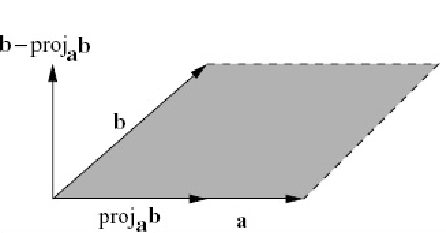
\includegraphics[height=2in]{2_ppgram}}
\caption{The parallelogram spanned by $\aa$ and $\bb$. \label{fig_ppgram}}
\end{figure}

\begin{eqnarray}
\nonumber 
A^2 & = & \|\aa\|^2\| \bb - (\aa\cdot\bb)\aa/\|\aa\|^2\|^2 \\
\nonumber 
    & = & \|\aa\|^2\left(
          \|\bb\|^2 + (\aa\cdot\bb)^2\|\aa\|^2/\|\aa\|^4 -
          2(\aa\cdot\bb)^2/\|\aa\|^2\right) \\
\nonumber 
    & = & \|\aa\|^2\|\bb\|^2 - (\aa\cdot\bb)^2 \\
\label{cross2}
    & = & (a_1^2+a_2^2+a_3^2)(b_1^2+b_2^2+b_3^2)-(a_1b_1+a_2b_2+a_3b_3)^2
\end{eqnarray}
Expanding the expressions in (\ref{cross1}) and (\ref{cross2}) reveals
that they are equal.

Notice that there are exactly two vectors satisfying properties 1 and
2, that is, perpendicular to the plane spanned by $\aa$ and $\bb$ and
of a given length. The cross product of $\aa$ and $\bb$ is the one
that satisfies the right hand rule. We say that vectors $\aa$, $\bb$
and $\cc$ (the order is important) satisfy the right hand rule if you
can point the index finger of your right hand in the direction of
$\aa$ and the middle finger in the direction of $\bb$ and the thumb in
the direction of $\cc$.  Try to convince yourself that if $\aa$, $\bb$
and $\cc$ (in that order) satisfy the right hand rule, then so do
$\bb$, $\cc$, $\aa$ and $\cc$, $\aa$, $\bb$.

Here are some properties of the cross product that are useful in doing
computations. The first two are maybe not what you expect.
\begin{enumerate}
\item $\aa\times\bb=-\bb\times\aa$
\item $\aa\times(\bb\times\cc)=(\cc\cdot\aa)\bb-(\bb\cdot\aa)\cc$.
\item $s(\aa\times\bb)=(s\aa)\times\bb=\aa\times(s\bb)$.
\item $\aa\times(\bb+\cc) = \aa\times\bb + \aa\times\cc$.
\item $\aa\cdot(\bb\times\cc)=(\aa\times\bb)\cdot\cc$.
\end{enumerate}

\begin{example}
\label{2008_a2_2} Let $\aa = (1,3,-2)$ and $\bb = (-1,2,3)$. Compute
the following:
{\begin{enumerate}
\renewcommand{\labelenumi}{(\alph{enumi})}
\item The area of the parallelogram whose sides are $\aa$ and $\bb$. 
\item The angle between $\aa$ and $\bb$. 
\end{enumerate}}
{\rm Solution:
\begin{enumerate}
\renewcommand{\labelenumi}{(\alph{enumi})}
\item The area of the parallelogram is equal to the length of 
$\aa \times \bb$:
\[
\aa \times \bb =  \left| \begin{array}{ccc}
\hat{i} & \hat{j} & \hat{k} \\
1 & 3 & -2 \\
-1 & 2 & 3
\end{array} \right| = \hat{i} (9+4) + \hat{j} (2-3) + \hat{k}(2+3) 
   = (13,-1,5) 
\]
so the area is 
\[
\| \aa \times \bb \| = \sqrt{13^2 + (-1)^2 + 5^2} = \sqrt{195} 
   \approx 13.96
\]
\item Note that the formula 
$\| \aa \times \bb \| = \| \aa \| \| \bb \| \sin \theta$ cannot be used 
for this question since it cannot distinguish between $\theta$ and 
$\pi - \theta$ (think about this point). Instead, use the $\cos$, dot 
product formula which should always be used for the calculation of 
angles between vectors unless you really know what you are doing:
\[
\cos \theta = \frac{\aa \cdot \bb}{\| \aa \| \| \bb \|} = 
\frac{(1,3,-2)\cdot (-1,2,3)}{\|(1,3,-2)\| \|(-1,2,3)\|} 
= \frac{-1+6-6}{\sqrt{1+9+4} \sqrt{1+4+9}} = \frac{-1}{14} 
\]
so 
\[
\theta = \cos^{-1} \left( \frac{-1}{14} \right) \approx 1.64 
   \mbox{\ radians or $\approx 94.10^\circ$}
\]
\end{enumerate}}
\end{example}

\begin{example}
Consider the triangle $T$ with three corners $(1,1,1)$, $(1,2,3)$ and $(2,0,1)$. Find the 
area of $T$. 
{\rm The area will be half of the area of the parallelogram spanned by (any) two 
distinct sides. We take sides $(1,2,3)-(1,1,1) = (0,1,2)$ and $(2,0,1) -(1,1,1) = (1,-1,0)$
which make the computations a bit easier. We compute 
\[
(0,1,2) \times (1,-1,0) = \det \left[ \begin{array}{ccc}
\hat{i} & \hat{j} & \hat{k} \\
0 & 1 & 2 \\
1 & -1 & 0
\end{array} \right] = (2, 2,-1) 
\]
and then the area of the triangle is 
\[
1/2 \| (2,2,-1) \| = 3/2. 
\] 
} 
\end{example} 
Try to convince yourself why it does not matter which two sides are taken in the computation above. 

\subsection{The triple product and the determinant in three dimensions}

The cross product is defined so that the dot product of $\aa$ with
$\bb\times\cc$ is a determinant:
\[
\aa\cdot(\bb\times\cc) = 
\det\left[\matrix{
	a_1&a_2&a_3\cr
	b_1&b_2&b_3\cr
	c_1&c_2&c_3\cr
}\right]
\]
This determinant is called the triple product of $\aa$, $\bb$ and
$\cc$.

Using this fact we can show that the absolute value of the triple
product is the volume of the parallelepiped spanned by $\aa$, $\bb$
and $\cc$.

A diagram of the parallepiped is shown in Figure~\ref{fig_triple}. 
The absolute value of the triple product is
\[
\left|\aa\cdot(\bb\times\cc)\right|
  = \|\aa\|\cos(\theta)\|\bb\times\cc\|.
\]
Here $\theta$ is the angle between $\aa$ and $\bb\times\cc$.
The quantity $\|\aa\|\cos(\theta)$ is the height of parallelepiped and
$\|\bb\times\cc\|$ is the area of the base. The product of these is
the volume of the parallepiped, as claimed. Thus
\[
\left|\det\left[\matrix{
	a_1&a_2&a_3\cr
	b_1&b_2&b_3\cr
	c_1&c_2&c_3\cr
}\right]\right|
=\mbox{Volume of the parallelepiped spanned by $\aa$, $\bb$ and $\cc$}
\]

\begin{figure}
\centerline{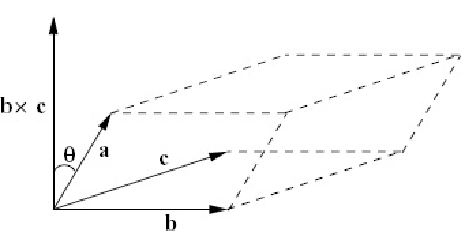
\includegraphics[height=2in]{2_triple}}
\caption{The Triple Product. \label{fig_triple}}
\end{figure}

The sign of the triple product is positive if $\theta$ is between
zero and $\pi/2$ and negative if $\theta$ lies between $\pi/2$ and
$\pi$.  This is the case if $\aa$ is on the same side of the plane
spanned by $\bb$ and $\cc$ as $\bb\times\cc$. This holds if the
vectors $\bb$, $\cc$ and $\aa$ (in that order) satisfy the right hand
rule. Equivalently $\aa$, $\bb$ and $\cc$ (in that order) satisfy the
right hand rule.

Mathematically, it is more satisfactory to define the right hand rule
using the determinant. That is, we say that vectors $\aa$, $\bb$ and
$\cc$ satisfy the right hand rule if the determinant
$\aa\cdot(\bb\times\cc)$ is positive.

\subsection{MATLAB: assigning matrices and {\tt det} and {\tt cross} 
commands}

\begin{description}
\item[{\tt cross}] The command {\tt cross(a,b)} computes the cross 
product $\aa \times \bb$. An error results if {\tt a} or {\tt b} are not 
vectors of length 3. As an example, the command
\begin{verbatim}
cross([1 0 0],[0 1 0])
\end{verbatim} 
gives the vector result [0 0 1]. 
\item[{\bf matrices:}] The syntax to generate a matrix is shown below using 
a $2 \times 2$ example
\begin{verbatim}
a = [1 2; 3 4]
\end{verbatim}
This command assigns a matrix to {\tt a} that has the vector [1 2] in its 
first row and [3 4] in its second. Entries of a matrix can be accessed 
individually, for example {\tt a(1,2)} is the entry in the first row, 
second column. 
\item[{\tt zeros}:] Many applications can lead to large 
matrices with many rows and columns. Even though MATLAB can do matrix 
computations, it can be tedious to enter these large matrices by hand. 
In some cases the matrices have mostly zeros as entries (these matrices 
are called {\em sparse}). In these cases it is more efficient to generate 
a matrix of all zeros and then modify the entries that are not zero. 
For example 
\begin{verbatim}
a = zeros(2,2);
a(1,1) = 1;
\end{verbatim}
generates a $2 \times 2$ matrix with entries that are all zero except the 
upper left entry which is 1. Note that {\tt zeros(n,m)} generates a 
matrix with $n$ rows and $m$ columns with all zero entries. 
So {\tt zeros(1,m)} is a row vector of length $m$ and {\tt zeros(n,1)}
is a column vector of length $m$ with all zero entries. 
\item[{\tt rand}:] {\tt rand (n,m)} generates a 
matrix with $n$ rows and $m$ columns with entries that are random numbers 
uniformly distributed in the interval [0,1].  
\item[{\tt det}:] The command {\tt det(a)} returns the determinant 
of the matrix {\tt a}. An error occurs if {\tt a} is not 
a square (same number of rows and columns) matrix. Determinants of 
larger matrices (than $2 \times 2$ and $3 \times 3$ discussed in this
section) are discussed in Chapter~\ref{ch_matrices_dets}.
\end{description}

\subsection{MATLAB: generating scripts with the MATLAB editor}

Often times using the command window in MATLAB to solve a problem can be tedious, because if the need arises to redo the problem, or change a parameter, one has to rewrite it all. The editor comes in handy for such cases. The editor is a text window (accesed from the command window: {\tt File $\rightarrow$ New $\rightarrow$ Blank M-file}) where one can write commands in the same syntax as the editor, and when one runs it, the results appear in the command window exactly as if one had written them there one after the other.

For example, the code to generate three random orthogonal vectors would look something like this:
\begin{verbatim}
a1 = rand(3,1)
b = rand(3,1);
a2 = cross(a1,b)
a3 = cross(a1,a2)
dot(a1,a2)
dot(a1,a3)
dot(a2,a3)
\end{verbatim}
Note that the last three lines are there to check that the three vectors are mutually orthogonal. Once the code was written, save it from the editor window: {\tt File $\rightarrow$ Save as}, making sure that the name of the file has a ``{\tt .m}'' extension (and the file name should contain no spaces). There are several different ways of running the script, the fastest one is to hit the {\tt F5} key. Alternatively, from the editor window it can be run from {\tt Debug $\rightarrow$ Run}, or directly from the command window by typing the name of the script into the MATLAB command line.

\subsection{MATLAB: floating point representation of real numbers}
\label{sec:floating}

MATLAB can represent integers exactly (up to limited but large size). Using a 
``floating point representation", MATLAB can represent 
most real numbers only approximately (but quite accurately - to 16 digits or so). In certain 
cases, the errors made in floating point approximation of numbers can be amplified 
and lead to noticeable errors in computed results. This will not happen typically in the 
examples and computer labs for Math 152, but the reader should be aware of the possibility. 

\begin{example} Consider the vectors 
\begin{eqnarray*}
{\bf a} & = & [1 \; 1 \; 1] \\
{\bf b} & = & [\sqrt{2} \; \sqrt{2} \; 0]
\end{eqnarray*}
and ${\bf c} = {\bf a} + {\bf b}$. 
If a $3 \times 3$ matrix $A$  is made with rows ${\bf a}$, ${\bf b}$ and ${\bf c}$ then 
the determinant of $A$ is zero (by construction, the vectors lie on the same plane). 
If this computation is done in MATLAB, 
\begin{verbatim}
a = [1 1 1];
b = [sqrt(2) sqrt(2) 0 ];
c = a + b;
A = [a; b; c];
det(A)
\end{verbatim}
the result is 3.1402e-16 not zero due to floating point approximation of intermediate 
computations. You can type {\tt eps} in MATLAB to see the maximum 
relative error made by 
floating point approximation. On the computer used to do the computation above, 
{\tt eps} had a value of 2.2204e-16, so it is believable that the calculation error in 
the determinant was made by the combination of a few floating point   approximations.
\end{example} 

Try to determine how many decimal digits of accuracy the floating point representation 
in your calculator uses (typically, the accuracy is greater than what is displayed). 

\subsection{Problems}

\begin{problem}
\label{op1_12}
Compute $[1,2,3]\times[4,5,6]$
\end{problem}

\begin{problem}
\label{2009_a2_1}
Use the definition to find the determinant of the matrix
\[
\left[ \begin{array}{ccc}
1 & 1 & 1 \\
1 & 2 & 3 \\
1 & 0 & -1
       \end{array} \right].
\]
Do the computation by hand showing your work, but you can check
your result using MATLAB.
From your result, decide if the vectors [1 1 1], [1 2 3] and [1 0 -1]
lie in the same plane (justify your answer, very briefly).
\end{problem}

\begin{problem}
\label{op1_13}
Verify that $\aa\cdot(\aa\times\bb)=0$ and $\bb\cdot(\aa\times\bb)=0$.
\end{problem}

\begin{problem}
\label{2008_a2_1} Simplify each of the following expressions:
{\begin{enumerate}
\renewcommand{\labelenumi}{(\alph{enumi})}
\item $((1,4,-1)\cdot(2,1,3)) ((2,1,4) \times (1,4,9))$
\item $(7,1,0)\cdot ((2,0,-1) \times (1,4,3))$
\item $(\aa \times \bb) \times (\bb \times \aa)$
\end{enumerate}}
\end{problem}

\begin{problem}
\label{op1_14}
Explain why $\|\aa\|\|\bb\|\sin(\theta)$ is the area of the
parallelogram spanned by $\aa$ and $\bb$. Here $\theta$ is the angle
between the two vectors.
\end{problem}

\begin{problem}
\label{op1_15}
Find examples to show that in general $\aa\times\bb\ne\bb\times\aa$
and $\aa\times(\bb\times\cc)\ne(\aa\times\bb)\times\cc$.
\end{problem}

\begin{problem}
\label{matlab_op1_15}
(Matlab) The Matlab command {\tt a=rand(1,n)} generates an $n\times 1$ vector with random entries. Write a script that generates three random vectors and write what you obtain from $\aa\times\bb-\bb\times\aa$,
and from $\aa\times(\bb\times\cc)-(\aa\times\bb)\times\cc$. Does that constitute a proof?
\end{problem}

\begin{problem}
\label{op1_16}
Show that $\aa\times(\bb\times\cc)=(\aa\cdot\cc)\bb-(\aa\cdot\bb)\cc$.
\end{problem}

\begin{problem}
\label{matlab_op1_16}
(Matlab) Write a script that generates three random vectors and checks that the result from problem \ref{op1_16} holds: $\aa\times(\bb\times\cc)=(\aa\cdot\cc)\bb-(\aa\cdot\bb)\cc$.
\end{problem}

\begin{problem}
\label{op1_17}
Derive an expression for $(\aa\times\bb)\cdot(\cc\times{\bf d})$ that
involves dot products but not cross products.
\end{problem}

\begin{problem}
\label{2008_a2_5}
{\begin{enumerate}
\renewcommand{\labelenumi}{(\alph{enumi})}
\item Draw a sketch containing the vectors $\aa$, $\bb$ and 
$\aa \times (\aa \times \bb)$. Assume that $\aa$ and $\bb$ lie in the 
plane of the paper and have an acute angle between them. 
\item Find a formula for $\aa \times (\aa \times \bb)$ which 
involves only $\| a \|$, $\bb$ and $\mbox{proj}_\aa \bb$. {\em Hint:} 
use a property of the dot product. 
\end{enumerate}}
\end{problem}

\begin{problem}
\label{op1_18}
What is the analog of the cross product in two dimensions? How about
four dimensions?
\end{problem}

\section{Lines and Planes} 

\subsection{Describing linear sets}

The following sections we will consider points, lines, planes and space
in two and three dimensions. Each of these sets have two complementary (or dual)
descriptions. One is is called the parametric form and the other the equation
form. Roughly speaking, the parametric form specifies the set using vectors
that are parallel to the set, while the equation form uses vectors that are
orthogonal to the set. Using the parametric description, it is easy to 
write down explicitly all the elements of the set, but difficult to check
whether a given point lies in the set. Using the equation description its the
other way around: if someone gives you a point, it is easy to check whether it
lies in the set, but it is difficult to write down explicitly even a single
member of the set. 

One way of thinking about solving a system of linear equations is simply going
from one description to the other. This will (hopefully) become clear later on.

These sections will always follow the same pattern. We will consider the
parametric and equation descriptions, first in the
special case when the set passes through the origin. Then we consider the
general case. 
Recall that when we say ``the point $\xx$'' this means ``the point at the head
of the vector $\xx$ whose tail is at the origin.''
In these sections we have used the notation $[x_1,x_2]$ instead of $[x,y]$ 
and $[x_1,x_2,x_3]$ instead of $[x,y,z]$ for typical points in two and three
dimensions.

\subsection{Lines in two dimensions: Parametric form}

First we consider lines passing through the origin.
Let $\aa=[a_1,a_2]$ be 
vector in the direction of the line. Then all the points $\xx$ on the line
are of the form 
\[
\xx = s\aa
\]
for some number $s$. The number $s$ is called a 
parameter. Every value of $s$ corresponds to exactly one point (namely $s\aa$) 
on the line.

Now we consider the general case. Let $\qq$ be a point on the line and $\aa$
lie in the direction of the line. Then the points on the line can be thought of
as the points on the line through the origin in the direction of $\aa$ shifted
or translated by $\qq$. Then a point $\xx$ lies on the line through
$\qq$ in the direction of $\aa$ exactly when 
\[
\xx=\qq+s\aa
\]
for some value of $s$.

\begin{example}
Find a parametric form of the line that goes through the points (1,2) and (2,4). 
{\rm We find the direction vector from 
\[
(2,4) - (1,2) = (1,2). 
\] 
Now 
\[
(1,2) + s (1,2) 
\]
is a parametric form of the line. That is, every point on the line can be written in the form above with a (unique) value of $s$ and every point of the form above is on the line. Note that parametric forms are not unique. The same line can be described by 
\[
(2,4) + t (2,4) 
\]
since we know the point (2,4) is on the line and the direction (2,4) is a scalar multiple of (1,2). Of course, specific points on the line will correspond to different values of $s$ and $t$. 
}
\end{example}



\subsection{Lines in two dimensions: Equation form}

First we consider lines passing through the origin shown in 
Figure~\ref{fig_line2d} (left).
Let $\bb=[b_1,b_2]$ be orthogonal to the direction of line. 
The point $\xx$ is on 
the line exactly when $\xx\cdot\bb=0$. This can be written
\[
x_1b_1 + x_2b_2 = 0.
\]

Now we consider the general case shown in 
Figure~\ref{fig_line2d} (right).
Let $\qq$ be a point on the line and
$\bb=[b_1,b_2]$ be orthogonal to the direction of line. A point $\xx$ lies on
the line through $\qq$ in the direction of $\aa$ exactly when $\xx-\qq$ lies
on the line through the origin in the direction of $\aa$. Thus
$(\xx-\qq)\cdot\bb =0$. This can be written
\[
(x_1-q_1)b_1 + (x_2-q_2)b_2 = 0
\]
or
\[
x_1b_1 + x_2b_2 = c,
\]
where $c=\qq\cdot\bb$. 

\begin{figure}
\centerline{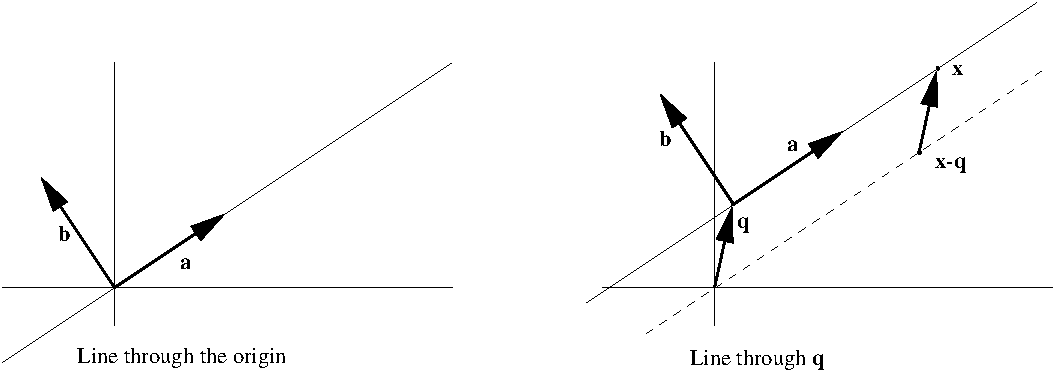
\includegraphics[height=1.5in]{2_line2d}}
\caption{A line in two dimensions. \label{fig_line2d}}
\end{figure}

\begin{example}
Find an equation form for the line in parametric form below:
\[
(1,2) + s (1,2).
\] 
{\rm We need to find a vector perpendicular to (1,2). We use the idea from section~\ref{s:trick}
and use 
\[
(1,2)^\perp = (-2,1) 
\]
Together with the point (1,2) on the line, we have an equation form 
\[
-x_1 + 2x_2 = (-2,1) \cdot (1,2) = 0 
\]
}
\end{example}

\begin{example} 
Find a parametric form for the line in equation form below:
\begin{equation}
\label{eq:2deqline} 
x_1 + 4 x_2 = 1. 
\end{equation} 
{\rm We need to find a point (any point) on the line. It is simple to look for the $x_2$ intercept ($x_2=0$) and find the point (1,0). The direction of the line will be perpendicular to (1,4) so we will use 
\[
(1,4)^\perp = (-4,1) 
\]
to get the parametric form 
\[
(x_1, x_2) = (1,0) + s(-4,1) 
\]
Note that for every $s$ we get a point that satisfies (\ref{eq:2deqline}). 
}
\end{example} 

\subsection{Lines in three dimensions: Parametric form}

The parametric form of a line in three (or higher) dimensions looks just
the same as in two dimensions. The points $\xx$ on the line are 
obtained by starting at
some point $\qq$ on the line and then adding all multiples 
of a vector $\aa$ pointing in the direction of the line. So
\[
\xx=\qq+s\aa
\]
The only difference is
that now $\qq$ and $\aa$ are vectors in three dimensions.

\begin{example} Find a parametric form for the line that passes through (1,1,1) and 
(1,2,3). Determine if the point (1,-2,3) is on the line. 
{\rm We find the direction of the line 
\[
(1,2,3) -(1,1,1) = (0,1,2) 
\]
so a parametric form of the line is 
\[
(1,1,1) + s(0,1,2). 
\]
If (1,-2,3) were on the line then 
\[
(1,1,1) + s(0,1,2) = (1,-2,3) 
\]
for some $s$. The above is a vector equation that must be satisfied for every component. The first component reads $1+0\times s = 1$ which is true for all $s$. The second component 
reads $1+s = -2$ which requires $s=-3$. If we now check the third component $1-3(2) = -5 \neq 3$. We conclude that (1,-2,3) is not on the line. 
}
\end{example}

\subsection{Lines in three dimensions: Equation form}

We begin with lines through the origin. A line through the origin can be
described as all vectors orthogonal to a plane. Choose two
vectors $\bb_1$ and $\bb_2$ lying in the plane that are not collinear (or zero).
Then a vector is orthogonal to the plane if and only if it is orthogonal to both
$\bb_1$ and $\bb_2$. Therefore the line consists of all points $\xx$ such that
$\xx\cdot\bb_1=0$ and $\xx\cdot\bb_2=0$. 
If $\bb_1=[b_{1,1},b_{1,2},b_{1,3}]$ and
$\bb_2=[b_{2,1},b_{2,2},b_{2,3}]$ then these equations can be written
\[
\matrix{
b_{1,1}x_1 &+ &b_{1,2}x_2 &+ &b_{1,3}x_3&= &0\cr
b_{2,1}x_1 &+ &b_{2,2}x_2 &+ &b_{2,3}x_3&= &0\cr
}
\]
Notice that there are many possible choices for the vectors $\bb_1$ and $\bb_2$.
The method of Gaussian elimination, studied later in this course, is a method of
replacing the vectors $\bb_1$ and $\bb_2$ with equivalent vectors in such a way
that the equations become easier to solve. 

Now consider a line passing through the point $\qq$  
and orthogonal to the directions
$\bb_1 $ and $\bb_2$ as shown in Figure~\ref{fig_line3d}. 
A point $\xx$ lies on this line precisely when $\xx-\qq$
lies on the line through the origin that is orthogonal to $\bb_1 $ and $\bb_2$.
Thus $(\xx-\qq)\cdot\bb_1=0$ and $(\xx-\qq)\cdot\bb_2=0$. This can be written
\[
\matrix{
b_{1,1}(x_1-q_1) &+ &b_{1,2}(x_2-q_2) &+ &b_{1,3}(x_3-q_3)&= &0\cr
b_{2,1}(x_1-q_1) &+ &b_{2,2}(x_2-q_2) &+ &b_{2,3}(x_3-q_3)&= &0,\cr
}
\]
or
\[
\matrix{
b_{1,1}x_1 &+ &b_{1,2}x_2 &+ &b_{1,3}x_3&= &c_1\cr
b_{2,1}x_1 &+ &b_{2,2}x_2 &+ &b_{2,3}x_3&= &c_2\cr
}
\]
where $c_1=\qq\cdot\bb_1$ and $c_2=\qq\cdot\bb_2$

\begin{figure}
\centerline{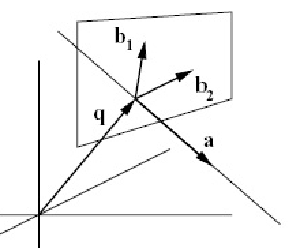
\includegraphics[height=2in]{2_line3d}}
\caption{A line in three dimensions. \label{fig_line3d}}
\end{figure}

\begin{example}
\label{ex:convert} 
Find a parametric and an equation form of the line that passes through the points (0,1,5) and (2,2,2).
{\rm We find a direction vector 
\[
{\bf v} = (2,2,2)-(0,1,5) = (2,1,-3)
\]
and write a parametric form for the line 
\[
{\rm \bf L:} {\bf x} = (0,1,5) + s(2,1,-3).
\]
To write an equation form we need to find two {\em different} (not collinear) vectors perpendicular to $\bf v$. To get one, we can use a variant of the procedure in Section~\ref{s:trick} where we rotated 2D vectors by 90$^\circ$ to get a perpendicular vector. 
\[
{\bf b_1} = (0, 3, 1).
\]
You can check directly that $\bf b_1$ is perpendicular to $\bf v$ (${\bf b_1} \cdot {\bf v} = 0$). To get the second vector $\bf b_2$ we can use the same idea on different components:
\[
{\bf b_2} = (-1,2,0).
\]
Note that ${\bf b_2}$ is perpendicular to $\bf v$ and not a multiple of $\bf b_1$ as required.  
An alternative for the second vector would be ${\bf b_1} \times \bf v$ since that vector is perpendicular to both $\bf v$ and $\bf b_1$. With the formulas above, we can write an equation form for the line:
\[
\matrix{
 & &3 x_2 &+ &x_3&= &8 \cr
-x_1 &+ &2x_2 & & &= &2.\cr
}
\]
You can check your answer by showing that both of the original points satisfy both equations. }
\end{example} 

\subsection{Planes in three dimensions: Parametric form}

We begin with planes through the origin. Since a plane is a two dimensional
object, we will need two parameters to describe points on the plane. Let $\aa_1$
and $\aa_2$ be non-collinear vectors in the direction of the plane. Then every
point on the plane can be reached by adding some multiple of $\aa_1$ to some
other multiple of $\aa_2$. In other words, points $\xx$ on the plane are 
all points of the form 
\[
\xx=s\aa_1+t\aa_2
\]
for some values of $s$ and $t$. 

If the plane passes through some point $\qq$ in the directions of $\aa_1$
and $\aa_2$, then we simply shift all the points on the parallel plane through
the origin by $\qq$. So $\xx$ lies on the plane if
\[
\xx=\qq+s\aa_1+t\aa_2
\]
for some values of $s$ and $t$. 

\begin{example} Find a parametric form of the plane that passes through the points (1,0,0), (1,1,1) and 
(1,0,2).
{\rm We find direction vectors 
\begin{eqnarray*}
{\bf a_1}  & = & (1,1,1)-(1,0,0) = (0,1,1) \\
{\bf a_2} & = & (1,0,2) - (1,0,0) = (0,0,2). 
\end{eqnarray*}
Note that $\bf a_1$ and $\bf a_2$ do not have the same direction (are not collinear). If they had been, then the three points would all be on the same line and so would not define a unique plane. We can proceed with the parametric form of the plane
\[
{\bf x} = (1,0,0) + s {\bf a_1} + t {\bf a_2} = (1, s, s+2t).
\]
}
\end{example}

\subsection{Planes in three dimensions: Equation form}

A plane through the origin can be described as all vectors orthogonal 
to a given vector $\bb$ as shown in Figure~\ref{fig_plane3d}. 
(In this situation, if $\bb$ has unit length it is called 
the normal vector to the plane and is often denoted ${\bf n}$.)
Therefore $\xx$ lies on the plane whenever $\xx\cdot\bb=0$, or
\[
\matrix{
b_{1}x_1 &+ &b_{2}x_2 &+ &b_{3}x_3&= &0.\cr
}
\]
If a plane with normal vector $\bb$ is translated so that it passes 
through the point $\qq$, then $\xx$
lies on the plane whenever $\xx-\qq$ lies on the parallel plane through the
origin. Thus $\xx$ lies on the plane whenever $(\xx-\qq)\cdot\bb=0$.
Equivalently
\[
\matrix{
b_{1}(x_1-q_1) &+ &b_{2}(x_2-q_2) &+ &b_{3}(x_3-q_3)&= &0,
}
\]
or
\[
\matrix{
b_{1}x_1 &+ &b_{2}x_2 &+ &b_{3}x_3&= &c,
}
\]
where $c=\qq\cdot\bb$.

\begin{figure}
\centerline{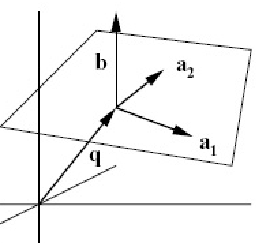
\includegraphics[height=2in]{2_plane3d}}
\caption{A plane in three dimensions. \label{fig_plane3d}}
\end{figure}

\begin{example}
Write the equation form of the plane described by the parametric form below:
\[
{\bf x} = (1+s+t, 5t, -2) 
\]
{\rm {\em Note:} It is possible to see the answer from the form above, but let us go through the steps of the calculations you would do if the example were more complicated. Write the expression above as 
\[
{\bf x} = (1,0,-2) + s(1,0,0) + t (1,5,0).
\]
In this form we can recognize ${\bf q} = (1,0,-2)$ as a point on the plane (corresponding to parameters $s=0$ and $t=0$) and the vectors ${\bf a}_1 = (1,0,0)$ and ${\bf a}_2 = (1,5,0)$ as directions {\em in} the plane. To write the equation form of the plane, we need a point on it (which we have) and the normal direction $\bf b$ to it, which must be perpendicular to ${\bf a}_1$ and ${\bf a}_2$. Thus we can compute 
\[
{\bf b} = {\bf a}_1 \times {\bf a}_2 = (0, 0, 5).
\]
Now the equation form of the plane is ${\bf b} \cdot {\bf x} = {\bf b} \cdot {\bf q}$ :
\[
0x + 0y + 5z = 0\cdot 1 + 0 \cdot 1 + 5 \cdot -2 = -10 
\mbox{\ \ \ or $z=-2$}   
\]
where in this case we have written the components of the vector $\bf x$ as $(x,y,z)$. }
\end{example} 

\begin{example}
Find a parametric form for the plane $x + y + 2z = 2$.
{\rm We identify the normal direction to the plane ${\bf b} = (1,1,2)$ by inspection. We need a point on the plane. It is easy to find one on the coordinate axes, (2,0,0) for example. To get two directions $\bf a_1$ and $\bf a_2$ in the plane, we need two different directions perpendicular to $\bf b$. Proceeding as in Example~\ref{ex:convert} we take 
\[
{\bf a_1} = (0,-2,1) \mbox{\ and \ } {\bf a_2} = (-1,1,0)
\]
leading to a parametric form 
\[
{\bf x} = (1,0,0) +s {\bf a_1} + t {\bf a_2} = (1-t, -2s+t, s) .
\]
}
\end{example}

\subsection{Problems}

\begin{problem}
\label{op1_21}
A line orthogonal to $\bb$ can be described as the set of all points $\xx$
whose projections onto $\bb$ all have the same value.
Using the formula for projections, show that this leads to the
equation description of the line.
\end{problem}

\begin{problem}
\label{op1_22}
Find both the parametric form and equation form for the line in Figure 
\ref{fig_lineprob}.
Write down five points on the line (notice that the parametric form is 
more useful for this). Check whether the point 
$[{{1012}\over{3}},{{1069}\over{21}}]$ is on the line
(notice that the equation form is more useful for this.)
\end{problem}

\begin{figure}
\centerline{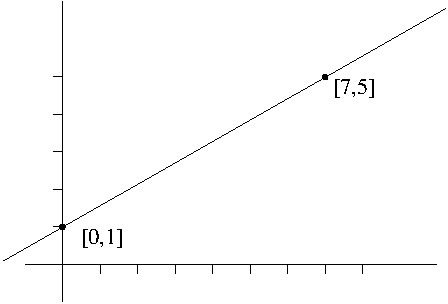
\includegraphics[height=1.5in]{2_lineprob}}
\caption{Diagram for problem \ref{op1_22}. \label{fig_lineprob}}
\end{figure}

\begin{problem}
\label{op1_23}
Find the equation form for the line $[1,1] + s[-1,2]$.
\end{problem}

\begin{problem}
\label{op1_24}
Find the parametric form for the line $x_1-3x_2=5$
\end{problem}

\begin{problem}
\label{op1_25}
Use a projection to find the distance from the point $[-2,3]$ to the line
$3x_1-4x_2=-4$
\end{problem}

\begin{problem}
\label{2009_a2_3}
Consider the plane $x-y+2z=7$.
\begin{enumerate}
\item What is the normal direction to the plane?
\item Find the coordinates of any point (your choice) on the plane.
\end{enumerate}
\end{problem}

\begin{problem}
\label{op1_26}
Let $\aa$, $\bb$ and $\cc$ be the vertices of a triangle. By definition, the
median of a triangle is a straight line that passes through a vertex of the
triangle and through the midpoint of the opposite side.
{\begin{enumerate}
\renewcommand{\labelenumi}{(\roman{enumi})}
\item Find the parametric form of the equation for each median.
\item Do all the medians meet at a common point? If so, which point?
\end{enumerate}}
\end{problem}

\begin{problem}
\label{2008_a2_3} Find a pair of equations which define the
line 
\[
\{ (2,0,-4) + s(0,1,3): s \in \mathbb{R} \}
\]
\end{problem}

\begin{problem}
\label{2008_a2_4} Find the intersection point between the line
\[
\{ (2,-1,6) + s(1,-1,0): s \in \mathbb{R} \}
\]
and the plane 
\[
\{ t(0,1,-3) + u(-1,2,0): t,u  \in \mathbb{R} \}
\]
{\em Hint:} first find an equation for the plane. 
\end{problem}

\begin{problem}
\label{2009_a2_4}
Find the intersection point of the line with parametric form
below
\[
(1,2,3) + t (1,0,-1)
\]
and the plane
\[
x + 2y - z = 5.
\].
\end{problem}

\begin{problem}
\label{op1_27}
Find the equation of the plane containing the points $[1,0,1]$, $[1,1,0]$ and
$[0,1,1]$.
\end{problem}

\begin{problem}
\label{op1_28}
Find the equation of the sphere which has the two planes $x_1+x_2+x_3=3$ and
$x_1+x_2+x_3=9$ as tangent planes if the centre of the sphere is on the planes
$2x_1-x_2=0$, $3x_1-x_3=0$.
\end{problem}

\begin{problem}
\label{2009_a2_5}
The planes $x+y+z = 2$ and $x-y+2z=7$ intersect in a line. Find
a parametric representation of this line. 
\end{problem}

\begin{problem}
\label{op1_29}
Find the equation of the plane that passes through the point $[-2,0,1]$ and
through the line of intersection of $2x_1+3x_2-x_3=0$, $x_2-4x_2+2x_3=-5$.
\end{problem}

\begin{problem}
\label{op1_30}
What's wrong with the question ``Find the equation for the plane containing 
$[1,2,3]$, $[2,3,4]$ and $[3,4,5]$.''?
\end{problem}

\begin{problem}
\label{op1_31}
Find the distance from the point $\pp$ to the plane $\bb\cdot\xx=c$.
\end{problem}

\begin{problem}
\label{op1_32}
Find the equation for the line through $[2,-1,-1]$ and parallel to each of the
two planes $x_1+x_2=0$ and $x_1-x_2+2x_3=0$. Express the equation fo the line
in both parametric and equation form.
\end{problem}

\begin{problem}
\label{matlab_op1_36}
(Matlab) Plotting figures in Matlab is quite simple. Simply type {\tt plot(1,2)} in the command window and observe what you get. Copy the following script (call it basicplot.m for example), and run it:
\begin{verbatim}
x = -2:0.1:2
m = 2
x_0 = 1
y_0 = 1
y = y_0 + m*(x-x_0)
plot(x,y,'.')
\end{verbatim}
Type {\tt help plot} in the command window to learn about different options for the plot command. Without closing the figure window, type {\tt hold on} in the command window, and re-run the script after changing the slope to {\tt m = -1/2} (the {\tt hold on} command allows you to overlap plots). Notice that the two lines should be perpendicular, but because of the scaling they appear not to be. Type in the command {\tt axis equal} to fix that. How would you modify the script to plot a circle of radius 3?

\end{problem}

\section{Introduction to Linear Systems}

\subsection{Description of points and the geometry of solutions to 
systems of equations}

So far we have considered the parametric and equation descriptions of lines and
planes in two and three dimensions. We can also try to describe points in the
same way. This will help you get a
geometric picture of what it means to solve a system of equations.

The ``parametric'' description of a point doesn't have any parameters! 
It simply is the name of the point $\xx=\qq$. 
In two dimensions the equation form for describing a point will look like
\[
\matrix{
b_{1,1}x_1 &+ &b_{1,2}x_2 &= &c_1\cr
b_{2,1}x_1 &+ &b_{2,2}x_2 &= &c_2\cr
}
\]
where the vectors $\bb_1=[b_{1,1},b_{1,2}]$ 
and $\bb_2=[b_{2,1},b_{2,2}]$ are not collinear (not multiples of each other).
Each equation describes a line. The point $\xx=[x_1,x_2]$ will
satisfy both equations if it lies on both lines, i.e., on the intersection. 
Since the vectors $\bb_1$ and $\bb_2$ are not co-linear, the
lines are not parallel, so the intersection is a single point. This situation 
is shown in Figure~\ref{fig_intersection}. 

\begin{figure}
\centerline{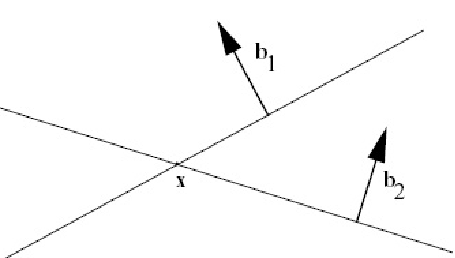
\includegraphics[height=1.5in]{2_intersection}}
\caption{Intersection of lines in 2D that are not collinear is a point.
\label{fig_intersection}}
\end{figure}

In three dimensions the equation form for describing a point will look like
\[
\matrix{
b_{1,1}x_1 &+ &b_{1,2}x_2 &+ &b_{1,3}x_3&= &c_1\cr
b_{2,1}x_1 &+ &b_{2,2}x_2 &+ &b_{2,3}x_3&= &c_2\cr
b_{3,1}x_1 &+ &b_{3,2}x_2 &+ &b_{3,3}x_3&= &c_3\cr
}
\]
where $\bb_1$, $\bb_2$ and $\bb_3$ don't all lie on the same plane. This can be
interpreted as the intersection of three planes in a single point.

Notice that going from the equation description of a point to the parametric
description just means finding the solution of the system of equations. If,
in two dimensions, the
vectors $\bb_1$ and $\bb_2$ are not collinear, or in three dimensions, 
$\bb_1$, $\bb_2$ and $\bb_3$ don't all lie on the same plane, then the system of
equations has a unique solution.

Now suppose that you are handed an arbitrary system of equations
\[
\matrix{
b_{1,1}x_1 &+ &b_{1,2}x_2 &+ &b_{1,3}x_3&= &c_1\cr
b_{2,1}x_1 &+ &b_{2,2}x_2 &+ &b_{2,3}x_3&= &c_2\cr
b_{3,1}x_1 &+ &b_{3,2}x_2 &+ &b_{3,3}x_3&= &c_3\cr
}
\]
What does the set of solutions $\xx=[x_1,x_2,x_3]$ look like?
As we just have seen, if $\bb_1$, $\bb_2$ and $\bb_3$ don't all lie on the same
plane, there is a unique solution given as the intersection of three planes.
Recall that the determinant can be used to test
whether the vectors $\bb_1$, $\bb_2$ and $\bb_3$ lie on the same plane. So a 
unique solution exists to the equation precisely when
\[
\det\left[\matrix{ b_{1,1}&b_{1,2}&b_{1,3}\cr
			b_{2,1}&b_{2,2}&b_{2,3}\cr
			b_{3,1}&b_{3,2}&b_{3,3}\cr}\right] \ne 0
\]
What happens when the determinant is zero and three 
vectors $\bb_1$, $\bb_2$ and $\bb_3$ do lie on 
the same plane? Then it could be that the three planes intersect in a line.
In this case every point on that line is a solution of the system of equations,
and the solution set has a parametric description of the form $\xx=\qq+s\aa$.
It could also be that all three planes are the same, in which case the solution
set is the plane. In this case the solution set has a parametric description of
the form $\xx=\qq+ s_1\aa_1+s_2\aa_2$
Another possibility is that two of the planes could 
be parallel with no intersection. In this case there are no solutions at all!
Some of these possibilities are illustrated in Figure~\ref{fig_planesint}.

\begin{figure}
\centerline{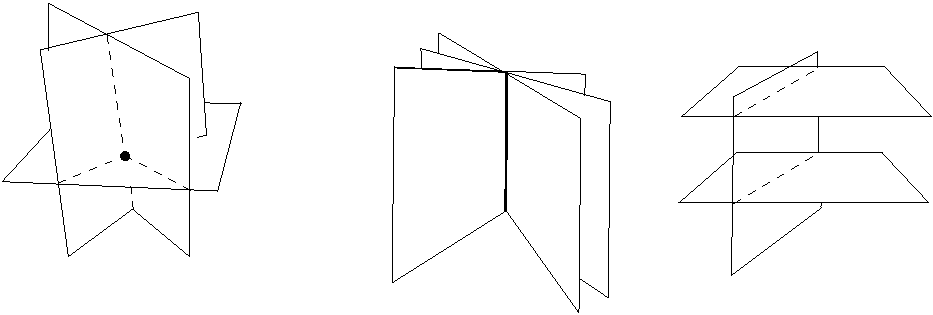
\includegraphics[height=1.5in]{2_planesint}}
\caption{Planes intersecting. \label{fig_planesint}}
\end{figure}

\begin{example} Determine whether the following system of linear equations has a solution. It is not 
necessary to find the solution or solutions if there are any. 
\[
\matrix{
x_1 &+ &x_2 &+ & x_3&= & 3 \cr
x_1 &+ &  &+ &2 x_3&= & 3 \cr
x_1 &+ &2 x_2 &+ &x_3&= & 4\cr
}
\]
{\rm We compute the determinant 
\[
\det\left[\matrix{ 1 & 1 & 1 \cr
			1 & 0 & 2 \cr
			1 & 2 & 1 \cr}\right] = -1 \ne 0
\]
Since the determinant is not zero, we know there is a unique solution point. By inspection, we can see that 
(1,1,1) solves all three equations and since we know this solution is unique, it is the only point that satisfies all three equations. In Chapter~\ref{ch:ch3} we will learn a systematic way to find the solution or all solutions (if any) of any linear systems. 
}
\end{example}

\begin{example} Determine whether the following system of linear equations has a solution. It is not 
necessary to find the solution or solutions if there are any. 
\[
\matrix{
x_1 &+ &x_2 &+ & x_3&= & 1 \cr
x_1 &+ &  &+ &x_3&= & 2 \cr
x_1 &+ &2 x_2 &+ &x_3&= & 1 \cr
}
\]
{\rm We compute the determinant 
\[
\det\left[\matrix{ 1 & 1 & 1 \cr
			1 & 0 & 1 \cr
			1 & 2 & 1 \cr}\right] = 0.
\]
Now we know that the system does not have a unique solution. Consider 
Figure~\ref{fig_planesint}. It can be made rigorous that there are two cases that could come from this system: either the solution describes a line (middle picture, infinite solutions) or the three planes do not intersect (right picture, no solutions). In Chapter~\ref{ch:ch3} we will develop an algorithm to decide this question. Here, we can look at combinations of the equations. Take twice the first equation and subtract the second to get 
\[
x_1 + 2x_2 +x_3 = 0.
\]
Since this contradicts the third equation, we see that this system has no solutions. 
}
\end{example}


\subsection{Describing the whole plane in two dimensions and all of 
space in three dimensions}

If the set we are trying to describe is the whole plane in two dimensions
or all of space in three dimensions,
then we don't need any equations, since there are no restrictions on the
points. However it does make sense to think about the parametric form. 

Lets start with two dimensions. Consider Figure~\ref{fig_basis}. 
If we pick any two vectors $\aa_1$ and $\aa_2$ that don't lie on the same line 
(that is they are different directions, not collinear),
then any vector $\xx=[x_1,x_2]$ in the plane can be 
written as $s_1\aa_1 + s_2\aa_2$. Notice that every choice of $s_1$ and $s_2$
corresponds to exactly one vector $\xx$. 
In this situation we could use the parameters
$s_1$ and
$s_2$ as co-ordinates instead of $x_1$ and $x_2$. In fact if $\aa_1$ and $\aa_2$
are unit vectors orthogonal to each other, this just amounts to changing the 
co-ordinate axes to lie along $\aa_1$ and $\aa_2$. The new co-ordinates
$[s_1,s_2]$ are then just what we were calling $[x'_1,x'_2]$ before. In fact,
even if the vectors $\aa_1$ and $\aa_2$
are not unit vectors orthogonal to each other, we can still think of them of 
lying along new co-ordinate axes. However, now the axes have been stretched and
sheared instead of just rotated, and need not lie at right angles any more. The discussion 
above motivates two important definitions. 

\begin{definition} 
A combination of vectors of the form 
\[
s_1\aa_1 + s_2\aa_2
\]
is called a {\rm linear combination} of $\{ \aa_1, \aa_2 \}$. The definition includes underlying sets of more vectors. That is, 
\[
s_1\aa_1 + s_2\aa_2 + s_3 \aa_3 
\]
is a linear combination of $\{ \aa_1, \aa_2, \aa_3 \}$ and so on. 
\end{definition} 
Writing vectors as linear combinations of a set of vectors has the interpretation of expressing the vector in a new coordinate system. 

\begin{definition} 
The set of all linear combinations of a set of vectors is called the {\rm span} of the set of vectors. 
\end{definition}

\begin{figure}
\centerline{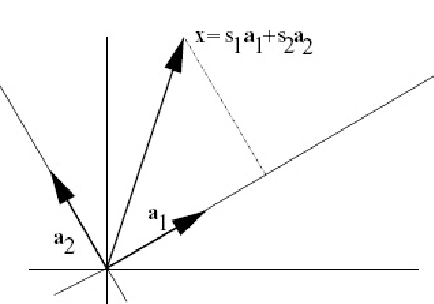
\includegraphics[height=1.5in]{2_basis}}
\caption{A basis in 2D \label{fig_basis}}
\end{figure}

The situation in three dimensions is similar. Now we must pick three vectors
$\aa_1$, $\aa_2$ and $\aa_3$ that don't lie on the same plane. Then every
vector
$\xx$ has a unique representation $\xx=s_1\aa_1+s_2\aa_2+s_3\aa_3$. We can say that the 
span of $\{ \aa_1, \aa_2, \aa_3 \}$ is all of $\mathbb{R}^3$. Again,
we could use $s_1$, $s_2$ and $s_3$ as co-ordinates in place of $x_1$, $x_2$ and
$x_3$. Again, if $\aa_1$, $\aa_2$ and $\aa_3$ are orthogonal with unit length,
then this amounts to choosing new (orthogonal) co-ordinate axes. 

\subsection{Linear dependence and independence}
\label{s:independence}

The condition in two dimensions that two vectors are not co-linear, and the 
condition in three dimensions that three vectors do not lie on the same plane
has now come up several times --- in ensuring that a system of equations has a
unique solutions and in ensuring that every vector can be written in a unique
way as a linear combination of those vectors. This condition can be tested by
computing a determinant.

We will now give this condition a name and define the analogous condition in
any number of dimensions.
Recall the definition that if $\aa_1, \aa_2, \ldots \aa_n$ is a collection of
vectors then a vector of the form 
\[
s_1\aa_1 + s_2\aa_2 + \cdots s_n\aa_n
\]
for
some choice of numbers $s_1, \ldots s_n$ is called a
{\it linear combination} of $\aa_1, \aa_2, \ldots \aa_n$.

\begin{definition}
A collection of vectors $\aa_1, \aa_2, \ldots \aa_n$ 
is called {\em linearly dependent} if some linear combination of them equals
zero, i.e., 
\[
s_1\aa_1 + s_2\aa_2 + \cdots s_n\aa_n =\zv
\]
for $s_1,\ldots s_n$ not all zero. A collection of vectors is said to be {\rm
linearly independent} if it is not linearly dependent. In other words, the
vectors $\aa_1, \aa_2, \ldots \aa_n$ are linearly independent if the only way a
linear combination of them $s_1\aa_1 + s_2\aa_2 + \cdots s_n\aa_n$ 
can equal zero is for $s_1=s_2=\cdots =s_n=0$.
\end{definition}

What does linear dependence mean in three dimensions? Suppose that $\aa_1$,
$\aa_2$ and $\aa_3$ are linearly dependent. Then there are some numbers
$s_1$, $s_2$ and $s_3$, not all zero, such that 
\[
s_1\aa_1 + s_2\aa_2 + s_3\aa_3=\zv.
\]
Suppose that $s_1$ is one of the non-zero numbers. Then we can
divide by $-s_1$ and find that 
$$-\aa_1+s_2'\aa_2 + s_3'\aa_3 =\zv$$ 
for
$s_2'=-s_2/s_1$ and $s_3'=-s_3/s_1$. Thus 
\[
\aa_1 = s_2'\aa_2 + s_3'\aa_3,
\]
or $\aa_1$ is a linear combination of $\aa_2$ and $\aa_3$. But this implies that
$\aa_1$ lies on the plane spanned by $\aa_2$ and $\aa_3$, i.e., the vectors
all lie on the same plane.  If $s_1$ happens to be 
zero we can repeat the same argument with one of the $s_i$'s which is not zero.
Thus linear dependence implies that all three vectors lie on the same plane. 
Conversely, if all three vectors lie on the same plane, then we can write one
vector as a linear combination of the other two, $\aa_1 = s_2'\aa_2 + s_3'\aa_3$
which implies $-\aa_1+s_2'\aa_2 + s_3'\aa_3 =\zv$ which says that the vectors
are linearly dependent. 

So in three dimensions, linear dependence means the vectors lie on the same
plane. 
Similarly, in two dimensions, linear dependence means the vectors are co-linear.

\begin{definition}
A collection of $n$ linearly independent 
vectors  $\aa_1, \aa_2, \ldots \aa_n$ in $\mathbb{R}^n$ dimensional space is called a
{\em basis}. 
If $\aa_1, \aa_2, \ldots \aa_n$ is a basis, then every vector 
$\xx$
can
be written in a unique way as a linear combination
\[
\xx=s_1\aa_1 + s_2\aa_2 + \cdots s_n\aa_n
\]
\end{definition} 

Two linearly independent vectors in 2D is a basis for $\mathbb{R}^2$. Three linearly independent vectors in 3D is a basis for $\mathbb{R}^3$. The span of two linearly independent vectors in $\mathbb{R}^3$ is a plane through the origin. This motivates the following:
\begin{definition}
The {\em dimension} of a span of a set $\cal C$ of linearly independent vectors is equal to the number of vectors in $\cal C$. 
\end{definition} 

\begin{example} Show that $(1,1)$ and $(2,0)$ are linearly independent. 
{\rm If they were linearly dependent by the definition they would be multiples of one another, which they are not. Thus, the vectors are linearly independent.  
}
\end{example} 

\begin{example} Write $(3,4)$ as a linear combination of $(1,1)$ and $(2,0)$.
{\rm From the previous example, we know that $(1,1)$ and $(2,0)$ are linearly independent, and so are a 
basis for $\mathbb{R}^2$ and so any vector in $\mathbb{R}^2$ can be written uniquely as a linear combination of them. We write 
\[
(3,4) = s(1,1) + t(2,0)
\]
or 
\begin{eqnarray*}
s + 2t & = & 3 \\
s + 0t & = & 4 
\end{eqnarray*}
It can be seen that writing a vector as a linear combination results in a linear system of equations. We will 
come back to this in Chapter~\ref{ch:ch3}. 
From the second component (second equation above), we see that $s=4$. Going to the first equation we can 
then determine $t= -1/2$. Thus 
\[
(3,4) = 4(1,1) -\frac{1}{2} (2,0)
\] 
}
\end{example} 

\begin{example} Show that $\{ (1,1,1), (1,1,2), (1,2,1) \}$ is a linearly independent set of vectors. 
{\rm We compute 
\[
\det\left[\matrix{ 1 & 1 & 1 \cr
			1 & 1& 2 \cr
			1 & 2 & 1 \cr}\right] = -1.
\]
Thus, the set of vectors is linearly independent. 
}
\end{example} 

\begin{example}
What is the dimension of the span of ${\cal C} = \{ (1,2,3,0), (1,1,1,1) \}$? 
{\rm By the definition of linear independence, two vectors can only be linearly dependent if they are multiples of each other. Thus, $\cal C$ is a linearly independent set and its span is two dimensional. It is a two dimensional set that includes the origin in $\mathbb{R}^4$. 
}
\end{example} 

\subsection{Problems}
%&&&

\begin{problem}
\label{op1_37}
Is the collection of vectors $\aa_1=[1,1]$, $\aa_2=[1,0]$ a basis for two
dimensional space? If so, express the vector $\xx=[0,1]$ as a linear combination
of $\aa_1$ and $\aa_2$
\end{problem}

\begin{problem}
\label{2008_a3_2} Let $\aa = [2,2,2]$ and $\bb = [3,4,1]$. Find
all vectors $\cc$ such that the list of vectors $\aa, \bb, \cc$ is 
{\em not} a basis of $\mathbb{R}^3$. 
\end{problem}

\begin{problem}
\label{2008_a3_1} Show that the collection of vectors $\aa = [1,1,1]$,
$\bb =[1,1,0]$ and $\cc = [1,0,0]$ is a basis of $\mathbb{R}^3$. Express 
$[1,2,3]$ as a linear combination of the vectors $\aa$, $\bb$ and $\cc$. 
\end{problem}

\begin{problem}
\label{2009_a3_1}
Let  the vectors ${\bf a} = [1,0,4]$, ${\bf b} = [2,-1,0] $and ${\bf c} = [8,-3,8]$. Do these vectors form a basis of $\mathbb{R}^3$? 
\end{problem}

\begin{problem}
\label{op1_38}
Is it possible for four vectors to be linearly independent in
three dimensional space?
\end{problem}

\begin{problem}
\label{2009_a3_2}
Show that the collection of vectors ${\bf a} = [2,1,3]$, ${\bf b} = [1,0,2] $ and ${\bf c} = [3,0,0]$ is a basis of $\mathbb{R}^3$. Express $[12, 2,4]$ as a linear combination of the vectors ${\bf a}, {\bf b}$ and ${\bf c}$.
\end{problem}

\begin{problem}
\label{op1_39}
Suppose that $\aa_1, \aa_2, \ldots \aa_n$ is a basis. Show that if some vector
$\xx$ has  representation $\xx=s_1\aa_1 + s_2\aa_2 + \cdots s_n\aa_n$
and $\xx=t_1\aa_1 + t_2\aa_2 + \cdots t_n\aa_n$, then $s_1=t_1$,
$s_2=t_2$,$\ldots$,$s_n=t_n$. (Hint: subtract the two expressions for $\xx$ and
use the fact that the basis vectors are linearly independent.)
\end{problem}

\begin{problem}
\label{matlab_op1_39}
(Matlab) Start by convincing yourself that the vectors $(1,3)$, and $(5,2)$ are linearly independent. This can easily be shown by writing a script that plots the vectors:
\begin{verbatim}
plot([1,0],[3,0])
hold on
plot([5,0],[2,0])
\end{verbatim}
We can extend this script by also plotting a linear combination of the two vectors:
\begin{verbatim}
alfa=1;
beta=1;
clf()
plot([alfa*1,0],[alfa*3,0])
hold on
plot([beta*5,0],[beta*2,0])
plot([alfa*1+beta*5,alfa*1],[alfa*3+beta*2,alfa*3],'--')
\end{verbatim}
Play around with the script and find parameters {\tt alfa} and {\tt beta} so that the vector $(1,1)$ can be written as a linear combination of $(1,3)$ and $(5,2)$.

\end{problem}

\section{Additional Topics}

These topics are not covered in the current version of Math 152 at UBC.

\subsection{Application: rotational motion}

Consider a rigid body rotating about an axis given by the unit vector
$\aa$ at a rate of $\Omega$ radians per second. Let $\rr$ be the
position vector of a point on the body as shown in Figure~\ref{fig_rotmot}.

\begin{figure}
\centerline{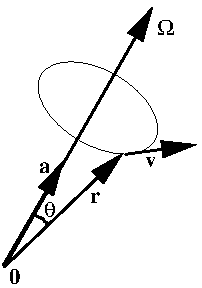
\includegraphics[height=2in]{2_rotmot}}
\caption{Rotational Motion. \label{fig_rotmot}}
\end{figure}

What is the velocity of the point? The point travels on a
circle with radius $\|\rr\|\sin(\theta)$, where $\theta$ is the angle that
$\rr$ makes with the axis. Therefore, in one second, the point travels a 
distance of $\Omega\|\rr\|\sin(\theta)$. Thus
{\begin{enumerate}
\renewcommand{\labelenumi}{(\roman{enumi})}
\item the magnitude of the velocity
is $\|{\bf v}\| = \Omega\|\rr\|\sin(\theta)$.
\item Now notice that ${\bf v}$ is
orthogonal to the plane spanned by $\aa$ and $\rr$.
\item Finally notice that $\Omega\aa$, $\rr$ and $\vv$ obey the right
hand rule.
\end{enumerate}}
The facts (i), (ii) and (iii) imply that $\vv$ is exactly the cross
product of $\Omega\aa$ and $\rr$. It is customary to let $\bf\Omega$
denote the vector $\Omega\aa$. Then
\[
{\bf v} = {\bf\Omega}\times\rr.
\]

\begin{problem}
\label{op1_19}
A body rotates at an angular velocity of $10$ rad/sec about the axis
through the points $[1,1,-1]$ and $[2,-3,1]$.  Find the velocity of
the point $[1,2,3]$ on the body.
\end{problem}

\begin{problem}
\label{2009_a2_2}
The line $L$ passing through the origin and the point
[1,1,1] passes through the midpoint of a thin metal rod of length
2 that is oriented in the direction [1,0,0]. The rod begins rotating
about $L$ at 3 revolutions per minute. What is the fastest speed
(length of velocity vector) of any point on the rod?
\end{problem}

\begin{problem}
\label{op1_20}
Imagine a plate that lies in the $xy$--plane and is rotating about the
$z$--axis. Let $P$ be a point that is painted on this plane. Denote by
$r$ the distance from $P$ to the origin, by $\theta(t)$ the angle at
time $t$ between the line from the origin to $P$ and the $x$--axis and
by $[x(t),y(t)]$ the co-ordinates of $P$ at the time $t$. Find $x(t)$
and $y(t)$ in terms of $\theta(t)$. Compute the velocity of $P$ in two
ways: 1. by differentiating $[x(t),y(t)]$ and 2. by computing
${\bf\Omega}\times\rr$.
\end{problem}

\subsection{Application: 3-D graphics}

How can we represent a three dimensional object on piece of paper or 
computer screen? Imagine the object in space and, a certain distance away,
a point $\pp$ representing the eye of the observer.
Between the observer and the object is a plane called the view plane.
The position of the origin of this plane is described by a point $\qq$, and its
orientation is given by three orthogonal unit vectors of length $1$, denoted
$\eee_1$, $\eee_2$ and $\eee_3$. (These are not the same as the standard basis
vectors $\ii$, $\jj$ and $\kk$ in this problem.) This situation is shown 
in Figure~\ref{fig_persp}. As usual, only the heads of the vectors 
(points) $\pp$, $\xx$, $\yy$ and $\qq$ are shown on the diagram. (The origin,
where the tails of these vectors lie, is not depicted at all.)
We will assume that the view plane is a distance one from the observer in the direction $\eee_3$.
Thus, $\eee_3$ can be thought of as the direction that the observer is looking.
Think of light rays leaving the object at point $\xx$ and travelling to the observer's eye
at $\pp$. At some point $\yy$ this line intersects the view plane. All the vectors $\yy$ on
the view plane that correspond to some vector $\xx$ on our object will furnish the two
dimensional representation of the object.

\begin{figure}
\centerline{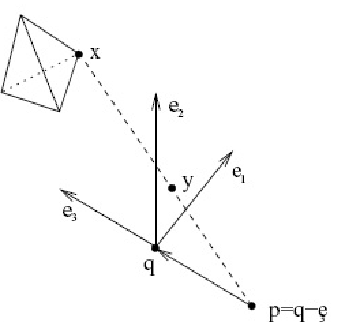
\includegraphics[height=2in]{2_persp}}
\caption{Perspective in 3-D graphics application. \label{fig_persp}}
\end{figure}

How do we determine the point $\yy$? The parametric
form of points on the plane is $\qq+s_1\eee_1+s_2\eee_2$. So we must have that
$\yy=\qq+s_1\eee_1+s_2\eee_2$ for some values of $s_1$ and $s_2$. We also know that
the vector $\xx-\pp$ is in the same direction as $\yy-\pp$. Therefore they must
be multiples, i.e., $\yy-\pp=\lambda(\xx-\pp)$ for some number $\lambda$.
Substituting in our expression for $\yy$ yields
\[
\qq+s_1\eee_1+s_2\eee_2-\pp=\lambda(\xx-\pp).
\]
Since $\qq-\pp=\eee_3$ this gives
\[
\eee_3+s_1\eee_1+s_2\eee_2=\lambda(\xx-\pp).
\]
Let us take the dot product of both sides of this equation with the unit vectors
$\eee_3$, $\eee_1$ and $\eee_2$. We can use the fact that $\eee_i\cdot\eee_j$ is zero
if $i\ne j$ and $1$ if $i=j$. Start with $\eee_3$. This gives
\[
\eee_3\cdot\eee_3 = 1 = \lambda\eee_3\cdot(\xx-\pp).
\]
This determines $\lambda$.
\[
\lambda = {{1}\over{\eee_3\cdot(\xx-\pp)}}.
\]
Now take the dot product with $\eee_1$. This gives
\[
s_1 = \lambda\eee_1\cdot(\xx-\pp) = {{\eee_1\cdot(\xx-\pp)}\over{\eee_3\cdot(\xx-\pp)}}
\]
Similarly, taking the dot product with $\eee_2$ leads to
\[
s_2= {{\eee_2\cdot(\xx-\pp)}\over{\eee_3\cdot(\xx-\pp)}}
\]

To plot the image of an object, we now simply plot the co-ordinates $s_1$ and
$s_2$  corresponding to all the points on the object on the $s_1$--$s_2$ plane.

\begin{example} Take $\pp=[11,0,0]$, $\qq=[10,0,0]$, $\eee_1=[0,1,0]$,
$\eee_2=[0,0,1]$ and $\eee_3=[-1,0,0]$. 
What is the image of the point $\xx=[1,1,1]$? 
{\rm 
We compute $\xx-\pp=[-10,1,1]$ so that
\begin{eqnarray*}
\eee_1\cdot(\xx-\pp) & = & 1 \\
\eee_2\cdot(\xx-\pp) &= & 1 \\
\eee_3\cdot(\xx-\pp) &= & 10
\end{eqnarray*}
So $s_1= s_2= 1/10$.}
\end{example}

\begin{example} Continue the previous example and 
compute the image of a line segment
between $[1,1,1]$ and $[2,0,1]$. {\rm 
These are all points of the form $\xx=[1,1,1]+
t([2,0,1]-[1,1,1]) = [1+t,1-t,1]$ as $t$ varies between $0$ and $1$.
This time we have $\xx-\pp=[1+t-11,1-t,1]$ so that
\begin{eqnarray*}
\eee_1\cdot(\xx-\pp) &= & 1-t \\
\eee_2\cdot(\xx-\pp) &= & 1 \\
\eee_3\cdot(\xx-\pp) &= & 10-t
\end{eqnarray*}
Thus $s_1 = (1-t)/(10-t)$ and $s_2=1/(10-t)$. Even though it is not immediately obvious,
the points $[s_1,s_2]$, as $t$ varies, all lie on a line segment. In fact 
\[
s_1 + 9 s_2 = (1-t)/(10-t)+9/(10-t) = (10-t)/(10-t) = 1.
\]
This shows that the points $[s_1,s_2]$ lie on a line perpendicular to $[1,9]$.}
\end{example}

In fact, it is possible to show that any line segment in space maps to a line
segment on the $s1$--$s2$ plane. Thus, to plot the image of an object consisting
of straight line segments (such as the tetrahedron in the picture) it is only
necessary to plot the vertices and then join them by straight lines.

\begin{problem}
\label{op1_33}
What are the $s_1$ and $s_2$ co=ordinates of the point $\xx=[1,2,3]$, if $\pp$,
$\qq$ are as above, $\eee_1=[0,1/\sqrt{2},1/\sqrt{2}]$ and 
$\eee_2=[0,-1/\sqrt{2},1/\sqrt{2}]$.
\end{problem}

\begin{problem}
\label{op1_34}
Plot the image on the $s_1$--$s_2$ plane of the tetrahedron whose 
vertices are located at
$[0,0,0]$, $[0,1,0]$, $[0,1/2,\sqrt{3}/2]$ and $[\sqrt{3}/6,\sqrt{6}/3,1/2]$
(Use the same values as before: $\pp=[-10,0,0]$, $\qq=[10,0,0]$, $\eee_1=[0,1,0]$,
$\eee_2=[0,0,1]$ and $\eee_3=[-1,0,0]$.)
\end{problem}

\begin{problem}
\label{op1_35}
Suppose that that points $\xx$ lie on the line $\xx=\xx_0 + t\vv$. 
Show that corresponding planar points $[s_1,s_2]$ also lie on a line. (Hint: show that
there are numbers $a$, $b$, $c$ that do not depend on $t$, so that $a s_1 + b s_2 = c$ for
every $t$.)
\end{problem}

\begin{problem}
\label{op1_36}
Consider a different drawing procedure where the point $\xx$ maps to the 
point on the view plane given by the intersection of the plane with the line
through $\xx$ parallel to $\eee_3$. Find a formula for the $s_1$ and $s_2$
co-ordinates of $\xx$.
\end{problem}

\section{Solutions to Chapter Problems}

%%%%%%%%%%%%%%%%%%%%%%%%%%%%%%%%%%%%%%%%%%%%%%%%%%%%%%%%%%%%%%%%%%%%%%%%%%%%%%%%
\noindent {\bf Solution \ref{2009_a1_1}} See Figure~\ref{2009_a1_1_sol}.

\begin{figure}[htb]
\centerline{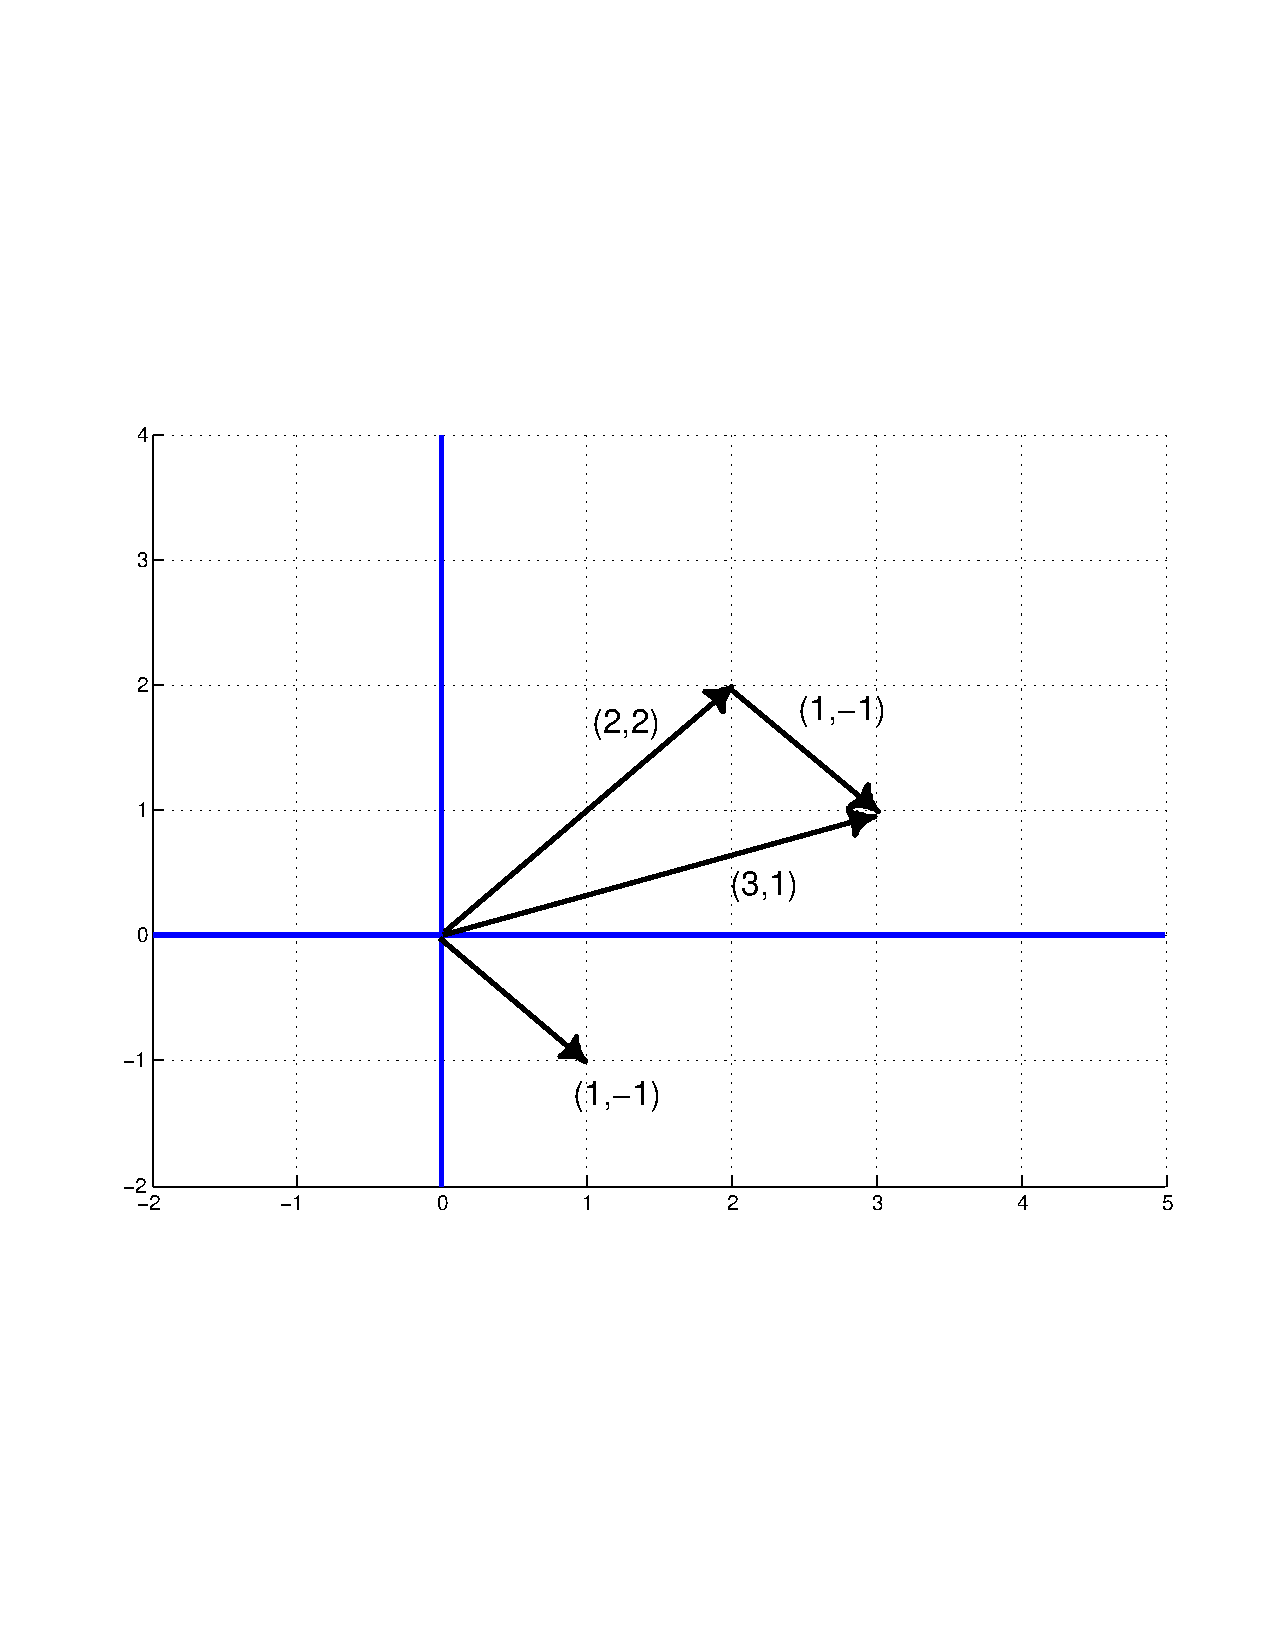
\includegraphics[height=3in]{2_2009_a1_1}}
\caption{Solution to problem \ref{2009_a1_1} \label{2009_a1_1_sol}}
\end{figure}

%%%%%%%%%%%%%%%%%%%%%%%%%%%%%%%%%%%%%%%%%%%%%%%%%%%%%%%%%%%%%%%%%%%%%%%%%%%%%%%%
\vspace{2mm}
\noindent {\bf Solution \ref{op1_1}}
{\begin{enumerate}
\renewcommand{\labelenumi}{(\roman{enumi})}
\item A straight line passing through the origin in the direction of $\aa$.
\item A ray (half line) passing through the origin in the direction of 
$\aa$.
\item A straight line parallel to $\aa$ passing through $\bb$.
\item If $\aa$ and $\bb$ do not lie on the same line:
a plane passing
through the origin parallel to $\aa$ and
$\bb$ (in two dimensions, this is the whole plane). 
If $\aa$ and $\bb$ lie on the same line: a
straight line passing through the origin in the direction of $\aa$ (and $\bb$).\par
\item If $\aa$ and $\bb$
both lie on the same line: a line passing through  $\cc$ parallel to
$\aa$ (and
$\bb$).  If $\aa$ and $\bb$ do not lie on the same line:
a plane passing
through $\cc$ parallel to $\aa$ and
$\bb$ (in two dimensions, this is the whole plane).
\end{enumerate}}

%%%%%%%%%%%%%%%%%%%%%%%%%%%%%%%%%%%%%%%%%%%%%%%%%%%%%%%%%%%%%%%%%%%%%%%%%%%%%%%%
\vspace{2mm}
\noindent {\bf Solution \ref{op1_2}}
$\aa-\bb$ is the vector that when added to $\bb$ gives $\aa$. So if we draw it
with its tail at $\bb$ then its head is at $\aa$. Similarly $\bb - \aa$ when
drawn with its tail at $\aa$ has its head at $\bb$.

%%%%%%%%%%%%%%%%%%%%%%%%%%%%%%%%%%%%%%%%%%%%%%%%%%%%%%%%%%%%%%%%%%%%%%%%%%%%%%%%

\vspace{2mm}
\noindent {\bf Solution \ref{op1_3}}
To find the midpoint we add half of the vector with its tail at $\aa$ and head
at $\bb$ to $\aa$. So the midpoint is $\aa + (1/2)(\bb-\aa)= (1/2)(\aa+\bb)$.
Similarly, the point one third of the way from $\aa$ to $\bb$ is
$\aa + (1/3)(\bb-\aa) = (2/3)\aa + (1/3)\bb$. 

%%%%%%%%%%%%%%%%%%%%%%%%%%%%%%%%%%%%%%%%%%%%%%%%%%%%%%%%%%%%%%%%%%%%%%%%%%%%%%%%
\vspace{2mm}
\noindent {\bf Solution \ref{op1_4}}
The line segment is given by the vectors $\aa + t(\bb-\aa)$ as $t$ varies
between $0$ and $1$.

%%%%%%%%%%%%%%%%%%%%%%%%%%%%%%%%%%%%%%%%%%%%%%%%%%%%%%%%%%%%%%%%%%%%%%%%%%%%%%%%
\vspace{2mm}
\noindent {\bf Solution \ref{2009_a1_2}}
$\aa = (1,2);\qquad \bb = (1,-2)$
{\begin{enumerate}
\renewcommand{\labelenumi}{(\alph{enumi})}
\item $\aa + \bb = (2,0)$
\item $2 \aa = (2,4)$
\item $\aa - \bb = (0,4)$
\item $\aa \cdot \bb = 1-4 = -3$.
\item $\| \bb \| = \sqrt{1 + 4} = \sqrt{5}$.
\end{enumerate}}

%%%%%%%%%%%%%%%%%%%%%%%%%%%%%%%%%%%%%%%%%%%%%%%%%%%%%%%%%%%%%%%%%%%%%%%%%%%%%%%%
\vspace{2mm}
\noindent {\bf Solution \ref{2008_a1_3}}
The radius of the circle is 
\[
\| (2,5) - (3,3) \| = \|(-1,2)\| = \sqrt{1+4} = \sqrt{5}.
\]
Thus using the standard equation for a circle 
\[
(x-2)^2 + (y-5)^2 = (\sqrt{5})^2 = 5.
\]

%%%%%%%%%%%%%%%%%%%%%%%%%%%%%%%%%%%%%%%%%%%%%%%%%%%%%%%%%%%%%%%%%%%%%%%%%%%%%%%%
\vspace{2mm}
\noindent {\bf Solution \ref{op1_5}}
The equation is $\|\xx-\aa\| = r$, or
\[
\sqrt{(x_1-a_1)^2+(x_2-a_2)^2+(x_3-a_3)^2} = r
\]
or
\[
(x_1-a_1)^2+(x_2-a_2)^2+(x_3-a_3)^2 = r^2
\]

%%%%%%%%%%%%%%%%%%%%%%%%%%%%%%%%%%%%%%%%%%%%%%%%%%%%%%%%%%%%%%%%%%%%%%%%%%%%%%%
\vspace{2mm}
\noindent {\bf Solution \ref{op1_6}}
The midpoint of the sphere is the midpoint of $[2,1,4]$ and $[4,3,10]$,
i.e., $(1/2)([2,1,4]+[4,3,10]) = [3,2,7]$. The radius is half the distance
between $[2,1,4]$ and $[4,3,10]$, i.e., \par $(1/2)\sqrt{(2-4)^2+(1-3)2+(4-10)^2} =
\sqrt{11}$. Thus the equation is
\[
(x_1-3)^2+(x_2-2)^2+(x_3-7)^2 = 11.
\]

%%%%%%%%%%%%%%%%%%%%%%%%%%%%%%%%%%%%%%%%%%%%%%%%%%%%%%%%%%%%%%%%%%%%%%%%%%%%%%%%
\vspace{2mm}
\noindent {\bf Solution \ref{op1_7}}
{\begin{enumerate}
\renewcommand{\labelenumi}{(\alph{enumi})}
\item $\aa\cdot\bb=-2+6=4$, $\theta = \arccos(4/(\sqrt{5}\sqrt{13})) =
1.05\ldots$
\item $\aa\cdot\bb= 1$, $\theta = 1.249\ldots$
\item $\aa\cdot\bb= 4$, $\theta = 0$
\item $\aa\cdot\bb= 2$, $\theta = 1.079\ldots\ldots$
\item $\aa\cdot\bb= 0$, $\theta = \pi/2\ldots$
\end{enumerate}}

%%%%%%%%%%%%%%%%%%%%%%%%%%%%%%%%%%%%%%%%%%%%%%%%%%%%%%%%%%%%%%%%%%%%%%%%%%%%%%%%
\vspace{2mm}
\noindent {\bf Solution \ref{2009_a1_4}}
Consider the dot product to determine angles between vectors, not the dot product (which only applies to 3D and cannot distinguish angles $\theta$ in the range $(0,\pi/2)$ from those in $(\pi/2,\pi)$, as discussed in the solution to problem \ref{op1_7} in the online notes).

\begin{enumerate}
\renewcommand{\labelenumi}{(\alph{enumi})}
\item $\aa = (1,1,1),\qquad \bb = (3,1,-2) \\ \aa\cdot\bb = 3+1-2 = 2\\
||\aa|| = \sqrt{3},\qquad ||\bb|| = \sqrt{3^2+1^2+(-2)^2}=\sqrt{14}.\\
\cos\theta = \frac{2}{\sqrt{3}\sqrt{14}},\qquad \theta = \cos^{-1}\frac{2}{\sqrt{3}\sqrt{14}}
\simeq 1.26 $ radians, or $\simeq 72.0^o$

\item Using $\aa\cdot\bb$ and $||\aa||$ above,\\
$proj_{\aa}\bb = \frac{2}{3}(1,1,1)=\left(\frac{2}{3},\frac{2}{3},\frac{2}{3}\right).$
Remember, $proj_{\aa}\bb$ should be in the direction of $\aa$.

\end{enumerate}

%%%%%%%%%%%%%%%%%%%%%%%%%%%%%%%%%%%%%%%%%%%%%%%%%%%%%%%%%%%%%%%%%%%%%%%%%%%%%%%%
\vspace{2mm}
\noindent {\bf Solution \ref{2008_a1_5}}
\begin{eqnarray*}
\aa = (1,4,0) & & \| \aa \| = \sqrt{17} \\
\bb = (2,-1,5) & & \| \bb \| = \sqrt{4 + 1 + 25} = \sqrt{30} 
\end{eqnarray*}
{\begin{enumerate}
\renewcommand{\labelenumi}{(\alph{enumi})}
\item $\cos \theta = \frac{\bb \cdot \aa}{\| \aa \| \| \bb \|} = 
   \frac{2-4}{\sqrt{17} \sqrt{30}} = \frac{-2}{\sqrt{510}}$ so
\[
\theta = \cos^{-1} \left( \frac{-2}{\sqrt{510}} \right) \approx 1.66 
\mbox{\ \ in radians or $\approx 95^\circ$}
\]
\item $\mbox{proj}_\aa \bb = \frac{\bb \cdot \aa}{\| \aa \|^2} \aa 
   = \frac{-2}{17} (1,4,0) = (-2/17, -8/17,0)$.
\end{enumerate}}

%%%%%%%%%%%%%%%%%%%%%%%%%%%%%%%%%%%%%%%%%%%%%%%%%%%%%%%%%%%%%%%%%%%%%%%%%%%%%%%%
\vspace{2mm}
\noindent {\bf Solution \ref{op1_8}}
The dot product is zero if $-1+2+s=0$, i.e., if $s=-1$.

%%%%%%%%%%%%%%%%%%%%%%%%%%%%%%%%%%%%%%%%%%%%%%%%%%%%%%%%%%%%%%%%%%%%%%%%%%%%%%%%
\vspace{2mm}
\noindent {\bf Solution \ref{op1_9}}
Let $\aa=[1,2,3]$, $\bb=[4,0,5]$ and $\cc=[3,4,6]$. The sides of the triangle
are in the directions of $\aa-\bb=[-3,2,-2]$, $\aa-\cc=[-2,-2,-3]$,
and $\bb-\cc=[1,-4,-1]$. To see if there
are any right angles we compute
$(\aa-\bb)\cdot(\aa-\cc)=[-3,2,-2]\cdot[-2,-2,-3]=8$,
$(\aa-\bb)\cdot(\bb-\cc)=[-3,2,-2]\cdot[1,-4,-1]=-9$ and
$(\aa-\cc)\cdot(\bb-\cc)=[-2,-2,-3]\cdot[1,-4,-1]=9$.
Since none of these are zero, there are no right angles.

%%%%%%%%%%%%%%%%%%%%%%%%%%%%%%%%%%%%%%%%%%%%%%%%%%%%%%%%%%%%%%%%%%%%%%%%%%%%%%%%
\vspace{2mm}
\noindent {\bf Solution \ref{2009_a1_5}}
If $[c_1, 1, c_2] = s[2, -2, 3]$, with $s$ a scalar multiple, then $s=-\frac{1}{2}$ (from the values in the second component), hence: \\
$c_1=-1,\qquad c_2 = -3/2$.

%%%%%%%%%%%%%%%%%%%%%%%%%%%%%%%%%%%%%%%%%%%%%%%%%%%%%%%%%%%%%%%%%%%%%%%%%%%%%%%%
\vspace{2mm}
\noindent {\bf Solution \ref{op1_10}}
The problem becomes much simpler if we choose the $y$ axis to run
along the runway and the x axis to run perpendicular to the runway. Replace
the wind and plane velocities by vectors ${\bf w}$ and ${\bf p}$ as on the
diagram in Figure~\ref{fig_plane}.

\begin{figure}
\centerline{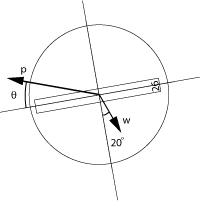
\includegraphics[height=2in]{2_plane}}
\caption{Coordinate system for Solution \ref{op1_10}. \label{fig_plane}}
\end{figure}

The wind vector has components $[-10\cos(20^\circ ), -10\sin(20^\circ )]$
while the plane velocity has components $[70\sin(\theta), 70\cos(\theta)]$.
We want the $x$ component to be zero hence we need
$10\cos(20^\circ)=70\sin(\theta)$. This gives $\theta = 7.7^\circ$, i.e,
the get the heading of the plane we have to add $7.7^\circ$ to the runway
direction. Thus the plane's heading is 267.7. The groundspeed is the magnitude
of the velocity, in this case simply the $y$ component given by
$70\cos(7.7^\circ)-10\sin(20^\circ)= 66$ knots.

%%%%%%%%%%%%%%%%%%%%%%%%%%%%%%%%%%%%%%%%%%%%%%%%%%%%%%%%%%%%%%%%%%%%%%%%%%%%%%%%
\vspace{2mm}
\noindent {\bf Solution \ref{op1_11}}
If we use the co-ordinate system where the $x$ axis is horizontal
and the $y$ axis is vertical, then the force of gravity is ${\bf F}_g=[0,-mg]$
The unit vector in the direction along the shaft is
${\bf p}=[-\sin(\theta),\cos(\theta)]$. The
force ${\bf F}_s$ exerted by the shaft is in the direction of the shaft,
hence a multiple of
${\bf p}$. So ${\bf F}_s = t{\bf p}$ for some number $t$. To find $t$ we use
that the component of the total force in the direction of the shaft must be
zero. Thus ${\rm proj}_{\bf p}{\bf F}_g +  {\bf F}_s = 0$, i.e.
${\bf p}\cdot{\bf F}_g + t=0$, i.e., $t=mg\cos(\theta)$. Thus the total force
is $ {\bf F}_g+{\bf F}_s=[0,-mg]+mg\cos(\theta)[-\sin(\theta),\cos(\theta)]
=mg[-\cos(\theta)\sin(\theta), -1+\cos^2(\theta)]$. Note that this is orthogonal
to ${\bf p}$, as it must be.

If we use co-ordinates where the $y$ axis runs along the shaft of the pendulum,
and the $x$ axis perpendicular to it, then
${\bf F}_g=[-mg\sin(\theta),-mg\cos(\theta)]$ while ${\bf F}_s=[0,t]$ for some
value of $t$. In this case it is simply the $y$ component that must be zero,
so $t=mg\cos(\theta)$ and ${\bf F}_g+{\bf F}_s=[-mg\sin(\theta),0]$

%%%%%%%%%%%%%%%%%%%%%%%%%%%%%%%%%%%%%%%%%%%%%%%%%%%%%%%%%%%%%%%%%%%%%%%%%%%%%%%%

\vspace{2mm}
\noindent {\bf Solution \ref{matlab_op1_11}}
\begin{verbatim}
sqrt(a(1)^2+a(2)^2)  
\end{verbatim}


%%%%%%%%%%%%%%%%%%%%%%%%%%%%%%%%%%%%%%%%%%%%%%%%%%%%%%%%%%%%%%%%%%%%%%%%%%%%%%%%

\vspace{2mm}
\noindent {\bf Solution \ref{op1_12}}
$[1,2,3]\times [4,5,6]=[-3,6,-3]$

%%%%%%%%%%%%%%%%%%%%%%%%%%%%%%%%%%%%%%%%%%%%%%%%%%%%%%%%%%%%%%%%%%%%%%%%%%%%%%%%
\vspace{2mm}
\noindent {\bf Solution \ref{2009_a2_1}}
\begin{eqnarray*}
\det \left[ \begin{array}{ccc}
	1& 1& 1 \\
	1& 2& 3 \\
	1& 0& -1
	    \end{array}
\right] &=& 1(-2-0) - 1(-1-3) + 1(0-2)\\
&=& -2+4-2 = 0
\end{eqnarray*}
Since the determinant is zero, the volume of the parallelepiped generated by the row vectors is zero. This implies that the vectors lie on the same plane.

%%%%%%%%%%%%%%%%%%%%%%%%%%%%%%%%%%%%%%%%%%%%%%%%%%%%%%%%%%%%%%%%%%%%%%%%%%%%%%%%
\vspace{2mm}
\noindent {\bf Solution \ref{op1_13}}
$\aa\cdot(\aa\times\bb) = [a_1, a_2, a_3]\cdot [a_2 b_3 - a_3 b_2, a_3 b_1- a_1 b_3,
a_1 b_2 - a_2 b_1] = a_1 a_2 b_3 - a_1 a_3 b_2 + a_2 a_3 b_1 - a_2 a_1 b_3
+ a_3 a_1 b_2 - a_3 a_2 b_1 = 0$. Now $\bb\cdot(\aa\times\bb) = -\bb\cdot(\bb\times\aa)
= 0$ by the previous calculation.

%%%%%%%%%%%%%%%%%%%%%%%%%%%%%%%%%%%%%%%%%%%%%%%%%%%%%%%%%%%%%%%%%%%%%%%%%%%%%%%%
\vspace{2mm}
\noindent {\bf Solution \ref{2008_a2_1}}
{\begin{enumerate}
\renewcommand{\labelenumi}{(\alph{enumi})}
\item $((1,4,-1)\cdot(2,1,3)) ((2,1,4) \times (1,4,9))$
\begin{eqnarray*}
 & = & (2+4-3) \left| \begin{array}{ccc} 
\hat{i} & \hat{j} & \hat{k} \\
2 & 1 & 4 \\
1 & 4 & 9 
\end{array} \right| \\
 & = & 3 (\hat{i} (9-16) + \hat{j}(4-18) + \hat{k}(8-1) \\
 & = & 3 (-7,-14,7) = (-21,-42,21) 
\end{eqnarray*}
\item $(7,1,0)\cdot ((2,0,-1) \times (1,4,3))$
\begin{eqnarray*}
 & = & (7,1,0) \cdot \left| \begin{array}{ccc}
\hat{i} & \hat{j} & \hat{k} \\
2 & 0 & -1 \\
1 & 4 & 3
\end{array} \right| \\
 & = & (7,1,0) \cdot (\hat{i} (0+4) + \hat{j}(-1-6) + \hat{k}(8-0) \\
 & = & (7,1,0) \cdot (4,-7,8) = 28-7+0 = 21
\end{eqnarray*}
\item $(\aa \times \bb) \times (\bb \times \aa)$
\[
= (\aa \times \bb) \times (- \aa \times \bb) = 
   - (\aa \times \bb) \times (\aa \times \bb) = {\bf 0} 
\]
because $\cc \times \cc = {\bf 0}$ for any vector $\cc$. 
\end{enumerate}}

%%%%%%%%%%%%%%%%%%%%%%%%%%%%%%%%%%%%%%%%%%%%%%%%%%%%%%%%%%%%%%%%%%%%%%%%%%%%%%%%
\vspace{2mm}
\noindent {\bf Solution \ref{op1_14}}
Here we are assuming that $\theta$ lies in $[0, \pi]$ so that $\sin(\theta)$ is
positive. The quantity $\|\aa\|$ is the length of the base of the parallelogram
while $\|\bb\|\sin(\theta)$ is the height. The area of a parallelogram is the
product of these. 

%%%%%%%%%%%%%%%%%%%%%%%%%%%%%%%%%%%%%%%%%%%%%%%%%%%%%%%%%%%%%%%%%%%%%%%%%%%%%%%%
\vspace{2mm}
\noindent {\bf Solution \ref{op1_15}}
Since $\aa\times\bb=-\bb\times\aa$ it is never true that
$\aa\times\bb=-\bb\times\aa$, unless $\aa\times\bb=\zv$. For the other example,
just try ${\bf i}$, ${\bf j}$ and ${\bf k}$. We have 
${\bf i}\times{\bf j}={\bf k}$ so 
${\bf i}\times({\bf i}\times{\bf j})={\bf i}\times {\bf k}=-{\bf j}$ On the other hand
$({\bf i}\times{\bf i})\times{\bf j}=\zv\times{\bf j}=\zv$

%%%%%%%%%%%%%%%%%%%%%%%%%%%%%%%%%%%%%%%%%%%%%%%%%%%%%%%%%%%%%%%%%%%%%%%%%%%%%%%%
\vspace{2mm}
\noindent {\bf Solution \ref{matlab_op1_15}}
\begin{verbatim}
a=rand(3,1);
b=rand(3,1);
c=rand(3,1);
cross(a,b) - cross(b,a)
cross(a,cross(b,c)) - cross(cross(a,b),c)
\end{verbatim}
This actually constitutes a proof, since we found a counter example. We don't have to show that it's always the case, we only had to show that in general the two assertions are not true.

%%%%%%%%%%%%%%%%%%%%%%%%%%%%%%%%%%%%%%%%%%%%%%%%%%%%%%%%%%%%%%%%%%%%%%%%%%%%%%%%
\vspace{2mm}
\noindent {\bf Solution \ref{op1_16}}
This a just a long calculation. One way to break it up is to consider $\aa=$ 
${\bf i}$, ${\bf j}$ and ${\bf k}$ separately. Suppose we can prove it for these
special cases. Then write a general 
$\aa$ as $a_1{\bf i}+a_2{\bf j}+a_3{\bf k}$. Then $\aa\times(\bb\times\cc)=
a_1{\bf i}\times(\bb\times\cc)+a_2{\bf j}\times(\bb\times\cc)
+a_3{\bf k}\times(\bb\times\cc)$ Assuming for the moment we know that the
special cases hold, then this equals $a_1((\ii\cdot\cc)\bb-(\ii\cdot\bb)\cc)
+a_2((\jj\cdot\cc)\bb-(\jj\cdot\bb)\cc) 
+ a_3((\kk\cdot\cc)\bb-(\kk\cdot\bb)\cc)= (\aa\cdot\cc)\bb-(\aa\cdot\bb)\cc$
Now we still have to prove the special cases. For example if $\aa=\ii$ we have
$\ii\times(\bb\times\cc) =
\det\left[\matrix{\ii&\jj&\kk\cr 1&0&0\cr
b_2c_3-b_3c_2&b_3c_1-b_1c_3&b_1c_2-b_2c_1\cr}\right]
=-(b_1c_2-b_2c_1)\jj+(b_3c_1-b_1c_3)\kk=[0,-b_1c_2+b_2c_1,b_3c_1-b_1c_3]
$ On the other
hand$(\ii\cdot\cc)\bb-(\ii\cdot\bb)\cc=c_1[b_1,b_2,b_3]-b_1[c_1,c_2,c_3]=
[0, c_1b_2-b_1c_2, c_1b_3-b_1c_3]$. The other two are similar.

%%%%%%%%%%%%%%%%%%%%%%%%%%%%%%%%%%%%%%%%%%%%%%%%%%%%%%%%%%%%%%%%%%%%%%%%%%%%%%%%
\vspace{2mm}
\noindent {\bf Solution \ref{matlab_op1_16}}
\begin{verbatim}
a=rand(3,1);
b=rand(3,1);
c=rand(3,1);
cross(a,cross(b,c)) - (dot(a,c)*b - dot(a,b)*c)
\end{verbatim}

%%%%%%%%%%%%%%%%%%%%%%%%%%%%%%%%%%%%%%%%%%%%%%%%%%%%%%%%%%%%%%%%%%%%%%%%%%%%%%%%
\vspace{2mm}
\noindent {\bf Solution \ref{op1_17}}
$(\aa\times\bb)\cdot(\cc\times\dd)=((\aa\times\bb)\times\cc)\cdot\dd$ (by
property 5) $= - (\cc\times(\aa\times\bb))\cdot\dd$ (by property 1)
$=-((\cc\cdot\bb)\aa+(\cc\cdot\aa)\bb)\cdot\dd
=-(\cc\cdot\bb)(\aa\cdot\dd)+(\cc\cdot\aa)(\bb\cdot\dd)$

%%%%%%%%%%%%%%%%%%%%%%%%%%%%%%%%%%%%%%%%%%%%%%%%%%%%%%%%%%%%%%%%%%%%%%%%%%%%%%%%
\vspace{2mm}
\noindent {\bf Solution \ref{2008_a2_5}}
{\begin{enumerate}
\renewcommand{\labelenumi}{(\alph{enumi})}
\item Let ${\bf v} = \aa \times (\aa \times \bb)$. Since $\aa \times \bb$ 
is orthogonal to the paper, $\bf v$ must lie in the plane of the paper. 
$\bf v$ is also orthogonal to $\aa$. Checking orientations with the 
right hand rule, there are only two sketches (up to rotation and resizing 
the vectors) shown in Figure~\ref{fig_newfig2}. 
\item $ \aa \times (\aa \times \bb)= 
(\bb \cdot \aa) \aa - (\aa \cdot \aa) \bb$ by property 2 in the notes. 
\[
 = \| \aa \|^2 \left( \frac{\bb \cdot \aa}{\| \aa \|^2} \aa - \bb \right) 
 = \| \aa \|^2(\mbox{proj}_\aa \bb - \bb).
\]
\end{enumerate}}

\begin{figure}
\centerline{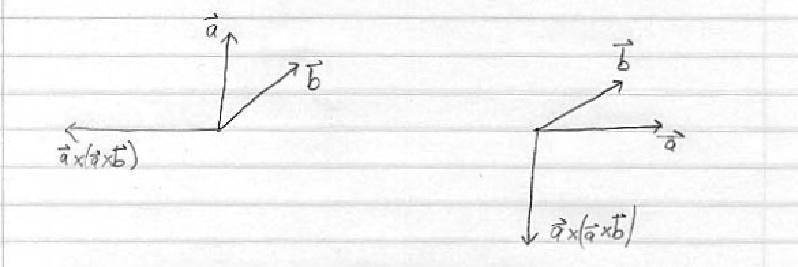
\includegraphics[height=1.5in]{2_newfig2}}
\caption{Vector sketch for the solution to \ref{2008_a2_5}.
\label{fig_newfig2}}
\end{figure}

%%%%%%%%%%%%%%%%%%%%%%%%%%%%%%%%%%%%%%%%%%%%%%%%%%%%%%%%%%%%%%%%%%%%%%%%%%%%%%%%
\vspace{2mm}
\noindent {\bf Solution \ref{op1_18}}
Actually there is no one right answer to this problem. But
in two dimensions the analog of the cross product could be an
operation on a single vector say $\times(\aa)$ with the property that
$\times(\aa)\cdot\bb=\det\left[\matrix{a_1&a_2\cr b_1&b_2\cr}\right]$ This
implies that $\times(\aa) = [a_2,-a_1]$. Note that $\times(\aa)$ is orthogonal
to $\aa$. The answer in $4$ dimensions is a little more obscure. In this case
the cross product could be an operation on three vectors 
that produces a vector that is orthogonal to all of them. One way of producing
such a vector would be to do the formal calculation of a $4\times 4$ determinant,
where the first row contains the four unit vectors $\eee_1$, $\eee_2$, $\eee_3$
and $\eee_4$, while the other three rows contain the entries of 
$\aa$,$\bb$ and $\cc$. Do you see why? 
(There is another possible, perhaps better answer, involving a different
type of product called the wedge product.)

%%%%%%%%%%%%%%%%%%%%%%%%%%%%%%%%%%%%%%%%%%%%%%%%%%%%%%%%%%%%%%%%%%%%%%%%%%%%%%%%
\vspace{2mm}
\noindent {\bf Solution \ref{op1_21}}
Let $\qq$ be a point on the line. Then the projection of $\xx$ in the direction
of $\bb$ is ${{\xx\cdot\bb}\over{\|\bb\|^2}}$. The set of all points whose
projection in the direction of $\bb$ are the same as the projection of the point
$\qq$ in the direction of $\bb$ is therefore the set of points $\xx$ such that
${{\xx\cdot\bb}\over{\|\bb\|^2}}={{\qq\cdot\bb}\over{\|\bb\|^2}}$. Multiplying
both sides by by $\|\bb\|^2$ gives $\xx\cdot\bb=\qq\cdot\bb$.

%%%%%%%%%%%%%%%%%%%%%%%%%%%%%%%%%%%%%%%%%%%%%%%%%%%%%%%%%%%%%%%%%%%%%%%%%%%%%%%%
\vspace{2mm}
\noindent {\bf Solution \ref{op1_22}}
The line is in the direction of $\aa=[7,5]-[0,1]=[7,4]$ and is therefore
perpendicular to $\bb=[4,-7]$. $\qq=[0,1]$ is a point on the line. So the
parametric form for the line is $[0,1]+s[7,4]$ and the equation form is
$4x_1-7x_2=-7$. So five points on the line are (picking $s=-2,1,0,1,2$)
$[-14,-7],[-7,-3],[0,1],[7,5],[14,9]$. To check whether $[1012/3,1069/21]$ lies
on the line, plug it into the equation: $4\cdot 1012/3-7\cdot 1069/21 \ne -7$
so the point does not lie on the line.

%%%%%%%%%%%%%%%%%%%%%%%%%%%%%%%%%%%%%%%%%%%%%%%%%%%%%%%%%%%%%%%%%%%%%%%%%%%%%%%%
\vspace{2mm}
\noindent {\bf Solution \ref{op1_23}}
We can take $\qq=[1,1]$ and $\bb=[2,1]$ so the equation is $2x_1+x_2=3$.

%%%%%%%%%%%%%%%%%%%%%%%%%%%%%%%%%%%%%%%%%%%%%%%%%%%%%%%%%%%%%%%%%%%%%%%%%%%%%%%%
\vspace{2mm}
\noindent {\bf Solution \ref{op1_24}}
We have to find a point on the line. Try for one of the form $[t,0]$. This
is on the line if $t-3\cdot 0=5$. So $[5,0]$ is on the line. The vector
orthogonal to the line is $[1,-3]$ so a vector parallel is $[3,1]$. Thus
the parametric form is $[5,0]+s[3,1]$.

%%%%%%%%%%%%%%%%%%%%%%%%%%%%%%%%%%%%%%%%%%%%%%%%%%%%%%%%%%%%%%%%%%%%%%%%%%%%%%%%
\vspace{2mm}
\noindent {\bf Solution \ref{op1_25}}
Pick a point $\qq$ on the line and let $\bb$ be orthogonal to the line. Then
the distance from a point $\xx$ to the line is the length of the
projection of $\xx-\qq$ onto $\bb$ as shown in Figure~\ref{fig_projl}.
\begin{figure}
\centerline{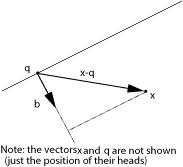
\includegraphics[height=2in]{2_projl}}
\caption{The projection used in Solution \ref{op1_25}. \label{fig_projl}}
\end{figure}
In this case we can take $\bb=[3,-4]$, $\qq=[0,1]$ and $\xx=[-2,3]$. The
projection is $((\xx-\qq)\cdot\bb/\|\bb\|^2)\bb$ This equals
$([-2,2]\cdot[3,-4]/25)[3,-4]=(-14/25)[3,4]$ The length of this vector
is $14/5$.

%%%%%%%%%%%%%%%%%%%%%%%%%%%%%%%%%%%%%%%%%%%%%%%%%%%%%%%%%%%%%%%%%%%%%%%%%%%%%%%%
\vspace{2mm}
\noindent {\bf Solution \ref{2009_a2_3}}
{\begin{enumerate}
\renewcommand{\labelenumi}{(\alph{enumi})}
\item the normal direction to the plane is $(1,-1,2)$
\item the point $(7,0,0)$ is on the plane (look for a solution with $y=z=0$ that is the intersection of the plane with the line of the x-axis).
\end{enumerate}}

%%%%%%%%%%%%%%%%%%%%%%%%%%%%%%%%%%%%%%%%%%%%%%%%%%%%%%%%%%%%%%%%%%%%%%%%%%%%%%%%
\vspace{2mm}
\noindent {\bf Solution \ref{op1_26}}
The midpoint between $\bb$ and $\cc$ is $(\bb+\cc)/2$. So the vector from
$\aa$ to this midpoint is $(\bb+\cc)/2-\aa$ and thus the parametric form for
the median is $\aa + t((\bb+\cc)/2-\aa)$. Similarly the parametric forms for the
other medians is $\bb + s((\aa+\cc)/2-\bb$ and $\cc + r((\aa+\bb)/2-\cc)$. When
$t=s=r=2/3$ these lines meet at the common point $(\aa+\bb+\cc)/3$

%%%%%%%%%%%%%%%%%%%%%%%%%%%%%%%%%%%%%%%%%%%%%%%%%%%%%%%%%%%%%%%%%%%%%%%%%%%%%%%%
\vspace{2mm}
\noindent {\bf Solution \ref{2008_a2_3}}
The line is in direction $(0,1,3)$. Two vectors which are orthogonal 
to the line are $(1,0,0)$ and $(0,3,-1)$, because $(1,0,0) \cdot (0,1,3) = 0$ 
and $(0,3,-1) \cdot (0,1,3) = 0$. Note that there are other choices for these 
two vectors that lead to different correct answers below. There will 
be two equations of the form 
\begin{eqnarray*}
x & = & c_1 \\
3y - z & = & c_2 
\end{eqnarray*}
Substituting the point $(2,0,4)$ that we know is on the line gives 
$c_1 = 2$ and $c_2 = 4$. Thus an equation form of the line is 
\begin{eqnarray*}
x & = & 2 \\
3y - z & = & 4 
\end{eqnarray*}

%%%%%%%%%%%%%%%%%%%%%%%%%%%%%%%%%%%%%%%%%%%%%%%%%%%%%%%%%%%%%%%%%%%%%%%%%%%%%%%%
\vspace{2mm}
\noindent {\bf Solution \ref{2008_a2_4}}
To find an equation for the plane we need an orthogonal vector 
\[
(0,1,-3) \times (-1,2,0)  =  \left| \begin{array}{ccc}
\hat{i} & \hat{j} & \hat{k} \\
0 & 1 & -3 \\
-1 & 2 & 0
\end{array} \right| = \hat{i} (0+6) + \hat{j} (3-0) + \hat{k}(0+1)
   = (6,3,1).
\]
So an equation for the plane is $6x + 3y + z = c$ and we know that 
$c=0$ since the plane goes through the origin. Any point on the line has the 
form 
\[
(2,-1,6) + s(1,-1,0) = (2+s, -1-s,6).
\]
Substituting this into the equation for the plane gives
\begin{eqnarray*}
6 (2+s) + 3(-1-s) + 6 & = & 0 \\
3s + 15 & = & 0 \\
s & = & -5 
\end{eqnarray*}
So the intersection point is 
\[
(2,-1,6) - 5(1,-1,0) = (2,-1,6)+(-5,5,0) = (-3,4,6). 
\]
{\em Note:} it can be checked that $t=-2$ and $u=3$ in the parametric form 
of the plane gives this point as well.

%%%%%%%%%%%%%%%%%%%%%%%%%%%%%%%%%%%%%%%%%%%%%%%%%%%%%%%%%%%%%%%%%%%%%%%%%%%%%%%%
\vspace{2mm}
\noindent {\bf Solution \ref{2009_a2_4}}
Points on the line satisfy
\begin{eqnarray*}
x &=& 1+t\\
y &=& 2\\
z &=& 3-t.
\end{eqnarray*}

To be on the plane, $x+2y-z=5$, or $(1+t) + 2(2) - (3-t) = 5$, or $2t+2=5$, or $t=3/2$.

Thus the intersection occurs at $(1,2,3) + (\frac{3}{2})(1,0,-1) = (\frac{5}{2},2,\frac{3}{2})$.

%%%%%%%%%%%%%%%%%%%%%%%%%%%%%%%%%%%%%%%%%%%%%%%%%%%%%%%%%%%%%%%%%%%%%%%%%%%%%%%%
\vspace{2mm}
\noindent {\bf Solution \ref{op1_27}}
Two vectors in the direction of the plane are $[1,1,0]-[1,0,1]=[0,1,-1]$ and
$[0,1,1]-[1,0,1]=[-1,1,0]$ To find a normal vector take the cross product
$[0,1,-1]\times[-1,1,0]=[1,1,1]$. So the equation of the plane is
$x_1+x_2+x_3=2$.

%%%%%%%%%%%%%%%%%%%%%%%%%%%%%%%%%%%%%%%%%%%%%%%%%%%%%%%%%%%%%%%%%%%%%%%%%%%%%%%%
\vspace{2mm}
\noindent {\bf Solution \ref{op1_28}}
The centre of the sphere lies in the plane halfway between the planes
$x_1+x_2+x_3=3$ and $x_1+x_2+x_3=9$. This is the plane $x_1+x_2+x_3=6$.
So the centre satisfies the three equations
\[
\matrix{
x_1     &+      x_2     &+      x_3     &=      6\cr
2x_1    &-      3x_2    &       &=      0\cr
3x_1    &       &-      x_3     &=      0\cr
}
\]
We will develop efficient techniques for solving such systems of equations.
For now, we can just use brute force: The second equation says $x_2=2x_1$ and
the third $x_3=3x_1$. Substituting this into the first equation yields$ x_1=1$,
so $x_2=2$ and $x_3=3$. Therefore the centre of the sphere is $[1,2,3]$. To
compute the radius, we must find the distance between the planes
$x_1+x_2+x_3=3$ and $x_1+x_2+x_3=6$ If we divide the equations by
$\|[1,1,1]\|=\sqrt{3}$, the first can be interpreted as vectors whose
projection onto the direction $\|[1,1,1]\|$ has length $3/\sqrt{3}=\sqrt{3}$,
the second can be interpreted as vectors whose
projection onto the direction $\|[1,1,1]\|$ has length $6/\sqrt{3}=2\sqrt{3}$.
The
radius is $\sqrt{3}$ so the equation is $(x_1-1)^2+(x_2-2)^2+(x_3-3)^2=3$.

%%%%%%%%%%%%%%%%%%%%%%%%%%%%%%%%%%%%%%%%%%%%%%%%%%%%%%%%%%%%%%%%%%%%%%%%%%%%%%%%
\vspace{2mm}
\noindent {\bf Solution \ref{2009_a2_5}}\\
$x+y+z = 2\qquad$ normal $(1,1,1)=\vec{b_1}$\\
$x-y+2z = 7\qquad$ normal $(1,-1,2)=\vec{b_2}$

The line direction can be found as 
\begin{eqnarray*}
  \vec{a} = \vec{b_1}\times\vec{b_2} = 
	\left[ \begin{array}{ccc}
\hat{i} & \hat{j} & \hat{k} \\
1 & 1 & 1 \\
1 &-1 & 2
\end{array} \right] = (3,-1,-2).
\end{eqnarray*}

We also need a point on the line. We can look for a point which has $z=0$ (the point that is the intersection of the line and the x-y plane). We get the two by two system

$$x+y=2 \mbox{, \ \ \ } 
x-y=7$$

Solving the system yields that $x=\frac{9}{2}$, and $y=-\frac{5}{2}$.

So $\left(\frac{9}{2}, -\frac{5}{2}, 0  \right) + s(3,-1,-2)$ is a parametric form of the line with parameter $s$.





%%%%%%%%%%%%%%%%%%%%%%%%%%%%%%%%%%%%%%%%%%%%%%%%%%%%%%%%%%%%%%%%%%%%%%%%%%%%%%%%
\vspace{2mm}
\noindent {\bf Solution \ref{op1_29}}
Set $x_2=0$ and solve $2x_1 -x_3=0$ and $x_1+2x_3=-5$ giving $x_1=-1$
and$x_2=-2$. This implies $[-1,0,-2]$ is in the plane we are looking for.
Set $x_3=0$ and solve $2x_1+3x_2=0x_1-4x_2=-5$ giving $x_1=-15/11$ and
$x_2=10/11]$ Hence $[-15/11,10/11,0]$ also lies on the plane. We now have
three points on the plane. Two vectors in the direction of the plane are
therefore  $[-2,0,1]-[-1,0,-2]=[-1,0,3]$
and$[-15/11,10/11,0]-[-1,0,-2]=[-4/11,10/11,2]$. Thus a normal vector is
$[-1,0,3]\times[-4/11,10/11,2]=[-30/11,10/11,-10/11]$ This is parallel to
$[-3,1,-1]$. Hence the equation is $-3x_1+x_2-x_3=5$.

%%%%%%%%%%%%%%%%%%%%%%%%%%%%%%%%%%%%%%%%%%%%%%%%%%%%%%%%%%%%%%%%%%%%%%%%%%%%%%%%
\vspace{2mm}
\noindent {\bf Solution \ref{op1_30}}
The three points are all on the same line. To see this, notice that the vectors
$[2,3,4]-[1,2,3]=[1,1,1]$ and $[3,4,5]-[1,2,3]=[2,2,2]$ are parallel.

%%%%%%%%%%%%%%%%%%%%%%%%%%%%%%%%%%%%%%%%%%%%%%%%%%%%%%%%%%%%%%%%%%%%%%%%%%%%%%%%
\vspace{2mm}
\noindent {\bf Solution \ref{op1_31}}
The distance of ${\bf p}$ to the plane $\bb\cdot\xx=c$ is the length of the
projection of ${\bf p}-\qq$ onto $\bb$, where $\qq$ is any point on the plane.
A point on the plane is $[c/b_1,0,0]$ (unless $b_1=0$ in which case we choose
either $[0,c/b_2,0]$ or $[0,0,c/b_3]$) The length of the
projection is $({\bf p}-\qq)\cdot\bb/\|\bb\|=(\bb\cdot{\bf p}-c)/\|b\|$.

%%%%%%%%%%%%%%%%%%%%%%%%%%%%%%%%%%%%%%%%%%%%%%%%%%%%%%%%%%%%%%%%%%%%%%%%%%%%%%%%
\vspace{2mm}
\noindent {\bf Solution \ref{op1_32}}
If the line is parallel to both planes, then it is orthogonal to both normal
vectors. Therefore $[1,1,0]\times[1,-1,2]=[2,-2,-2]$ is in the direction of
the line. Therefore the parametric form of the line is $[2,-1,-1]+s[2,-2,-2]$
The two equations are $x_1+x_2=[1,1,0]\cdot[2,-1,-1]=1$ and
$x_1-x_2+2=[1,-1,2]\cdot[2,-1,-1]=1$.

%%%%%%%%%%%%%%%%%%%%%%%%%%%%%%%%%%%%%%%%%%%%%%%%%%%%%%%%%%%%%%%%%%%%%%%%%%%%%%%%
\vspace{2mm}
\noindent {\bf Solution \ref{matlab_op1_36}}
\begin{verbatim}
x=-3:0.1:3
y = sqrt(9-x.^2)
plot(x,y,'.')
hold on
plot(x,-y,'.')
axis equal
\end{verbatim}

%%%%%%%%%%%%%%%%%%%%%%%%%%%%%%%%%%%%%%%%%%%%%%%%%%%%%%%%%%%%%%%%%%%%%%%%%%%%%%%%
\vspace{2mm}
\noindent {\bf Solution \ref{op1_37}}
Yes $[1,1]$ and $[1,0]$ do form a basis, since they don't lie on the same line.
(By the way, there is some potential for confusion here. When I say here that
$[1,1]$ and $[1,0]$ don't lie on the same line, I'm thinking of them as position
vectors, drawn with their tails at the origin. It probably would be more clear
to say that the vectors are not parallel.) Every vector in the plane can be
written as a linear combination of these two. In particular $[0,1]=[1,1]-[1,0]$

%%%%%%%%%%%%%%%%%%%%%%%%%%%%%%%%%%%%%%%%%%%%%%%%%%%%%%%%%%%%%%%%%%%%%%%%%%%%%%%%
\vspace{2mm}
\noindent {\bf Solution \ref{2008_a3_2}}
Note that $\aa$ and $\bb$ are linearly independent (they are not multiples 
of one another). So $\aa$, $\bb$ and $\cc$ will be linearly independent and 
so a basis for $\mathbb{R}^3$ {\em unless} $\cc$ is a linear 
combination of $\aa$ and $\bb$, that is it can be written as 
\[
\cc = r \aa + s \bb
\]
for some $r$ and $s$. 

%%%%%%%%%%%%%%%%%%%%%%%%%%%%%%%%%%%%%%%%%%%%%%%%%%%%%%%%%%%%%%%%%%%%%%%%%%%%%%%%
\vspace{2mm}
\noindent {\bf Solution \ref{2008_a3_1}}
The collection is a basis if the vectors are linearly independent. We 
consider $r \aa + s \bb + t \cc = \bf 0$ which leads to 
\begin{eqnarray*}
r + s + t & = & 0 \\
r + s & = & 0 \\
r & = & 0 
\end{eqnarray*}
Starting from the last equation and working up, we see that $r=0$, $s=0$, 
and $t=0$ which shows that the vectors are linearly independent and 
therefore form a basis. The linear independence could also have been 
shown by considering the determinant 
\[
\left| \begin{array}{ccc} 1 & 1 & 1 \\ 1& 1 & 0 \\ 1 & 0 & 0 \end{array}
\right| = 1 \neq 0 
\]
Since the determinant is not zero the vectors do not lie on the same plane 
and so are linearly independent. To write $[1,2,3]$ as a linear 
combination 
\[
[1,2,3] = r[1,1,1] + s [1,1,0] + t [1,0,0] 
\]
match components working backwards to get successively $r=3$, $s=-1$ 
and $t=-1$.

%%%%%%%%%%%%%%%%%%%%%%%%%%%%%%%%%%%%%%%%%%%%%%%%%%%%%%%%%%%%%%%%%%%%%%%%%%%%%%%%
\vspace{2mm}
\noindent {\bf Solution \ref{2009_a3_1}}
The vectors $\aa$, $\bb$, and $\cc$ are vectors in 3-D. Thus they form a basis if and only if they are linearly independent.

The three vectors are linearly independent if and only if the matrix $A$ with rows given by the three vectors satisfies
$$\det(A)\neq 0.$$
Here
$$
A = \left[\begin{array}{ccc} 1 & 0 & 4 \\ 2& -1 & 0 \\ 8 & -3 & 8 \end{array}\right]
$$
%%%%%%%%%%%%%%%%%%%%%%%%%%%%%%%%%%%%%%%%%%%%%%%%%%%%%%%%%%%%%%%%%%%%%%%%%%%%%%%%
\vspace{2mm}
\noindent {\bf Solution \ref{op1_38}}
No, it is not possible for four vectors to be linearly independent in three
dimensional space. To see this, first notice that if four vectors are
linearly independent any subset of three  vectors
must also be linearly independent (If three vectors would lie on the same plane,
we could find a non-trivial linear combination of those three equal to zero.
Then by adding $0$ times the left over vector, we would get a non-trivial linear
combination of all four vectors equal to zero, contradicting their
independence.)
But this means that those three vectors form a basis for three
dimensional space. So the fourth vector must be expressible as a linear
combination of the first three. This means the four vectors are not independent.

%%%%%%%%%%%%%%%%%%%%%%%%%%%%%%%%%%%%%%%%%%%%%%%%%%%%%%%%%%%%%%%%%%%%%%%%%%%%%%%%
\vspace{2mm}
\noindent {\bf Solution \ref{2009_a3_2}}
It is enough to check that $\det(A)\neq 0$. We have that
$$
A = \left[\begin{array}{ccc} 2 & 1 & 3 \\ 1& 0 & 2 \\ 3 & 0 & 0 \end{array}\right],\qquad
\det(A) = 6\neq 0,
$$
so they form a basis. We want to find $s_1$, $s_2$, and $s_3$ such that
$$
\left(\begin{array}{c} 12 \\ 2 \\ 4\end{array}\right) = s_1\left(\begin{array}{c} 2 \\ 1 \\ 3\end{array}\right) + s_2\left(\begin{array}{c} 1 \\ 0 \\ 2\end{array}\right) + s_3\left(\begin{array}{c} 3 \\ 0 \\ 0\end{array}\right).
$$
We have the following system of equations:
\begin{eqnarray*}
  12 &=& 2s_1 + s_2 + 3s_3\\
	2 &=& s_1 \\
	4 &=& 3s_1 + 2s_2
\end{eqnarray*}
% 
Hence $s_1=2$, $s_2 = -1$, $s_3 = 3$.

%%%%%%%%%%%%%%%%%%%%%%%%%%%%%%%%%%%%%%%%%%%%%%%%%%%%%%%%%%%%%%%%%%%%%%%%%%%%%%%%
\vspace{2mm}
\noindent {\bf Solution \ref{op1_39}}
If $\xx=s_1\aa_1 + s_2\aa_2 + \cdots s_n\aa_n$ and
$\xx=t_1\aa_1 + t_2\aa_2 + \cdots t_n\aa_n$, then $\zv=\xx-\xx
=(s_1-t_1)\aa_1 + (s_2-t_2)\aa_2 + \cdots (s_n-t_n)\aa_n$. Since the vectors
$\aa_1, \aa_2, \ldots \aa_n$ are linearly independent, the only way this
can happen is $s_1-t_1=0, \ldots, s_n-t_n=0$, or $s_1=t_1, \ldots, s_n=t_n.$

%%%%%%%%%%%%%%%%%%%%%%%%%%%%%%%%%%%%%%%%%%%%%%%%%%%%%%%%%%%%%%%%%%%%%%%%%%%%%%%%
\vspace{2mm}
\noindent {\bf Solution \ref{matlab_op1_39}}
The values {\tt alpha = 0.23, beta = 0.15} provide a good approximation to the linear combination.

%%%%%%%%%%%%%%%%%%%%%%%%%%%%%%%%%%%%%%%%%%%%%%%%%%%%%%%%%%%%%%%%%%%%%%%%%%%%%%%%
\vspace{2mm}
\noindent {\bf Solution \ref{op1_19}}
The axis is parallel to $[2,-3,1]-[1,1,-1]=[1,-4,2]$. The unit vector in this 
directions is $1/\sqrt{21}[1,-4,2]$ (Actually there is an ambiguity in the
problem: the unit vector could also point in the opposite direction. This would
change the sign of the answer.) So ${\bf \Omega}=(10/\sqrt{21})[1,-4,2]$. The 
vector $\rr$ has its tail co-inciding with the tail of $\Omega$ and its head
at $[1,2,3]$. So $\rr=[1,2,3]-[1,1,-1]=[0,1,4]$ and the
velocity is ${\bf v}={\bf \Omega}\times[0,1,4]=(10/\sqrt{21})[-18,-4,1]$

%%%%%%%%%%%%%%%%%%%%%%%%%%%%%%%%%%%%%%%%%%%%%%%%%%%%%%%%%%%%%%%%%%%%%%%%%%%%%%%%
\vspace{2mm}
\noindent {\bf Solution \ref{2009_a2_2}}
Some preliminary discussion:
{\begin{enumerate}
\renewcommand{\labelenumi}{(\roman{enumi})}
\item it does not matter where the centre of the rod is along L, we can take it to be at the origin for convenience.
\item the fastest speed is at the rod tip, and this does not change in time, so
\item it is OK to evaluate the speed at the initial position.
\end{enumerate}}
% 
$\Omega = 3\cdot 2\pi = 6\pi$ radians/min.

$\hat{a} = \frac{1}{\sqrt{3}}(1,1,1)$ unit vector in the direction of the axis of rotation.

$\vec{v} = \Omega\hat{a}\times\vec{r} = \frac{6\pi}{\sqrt{3}}(1,1,1)\times(1,0,0)$, with $\vec{r}$ the initial position of the tip.

Now evaluate the cross product:
\begin{eqnarray*}
 \left[ \begin{array}{ccc}
\hat{i} & \hat{j} & \hat{k} \\
1 & 1 & 1 \\
1 & 0 & 0
\end{array} \right] = (0,1,-1),
\end{eqnarray*}

so $\vec{v} = \frac{6\pi}{\sqrt{3}}(0,1,-1)$, and hence the speed is $||v|| = 2\pi\sqrt{6}$m/min

%%%%%%%%%%%%%%%%%%%%%%%%%%%%%%%%%%%%%%%%%%%%%%%%%%%%%%%%%%%%%%%%%%%%%%%%%%%%%%%%
\vspace{2mm}
\noindent {\bf Solution \ref{op1_20}}
We have $[x(t),y(t),0]$ $=r[\cos(\theta(t)),\sin(\theta(t)),0]$ so the velocity
is 
\begin{eqnarray*}
[\dot x(t),\dot y(t),0] &= & 
r[-\sin(\theta(t))\dot\theta(t),\cos(\theta(t))\dot\theta(t),0] \\
&= & 
r\dot\theta(t)[-\sin(\theta(t)),\cos(\theta(t)),0]
\end{eqnarray*}
On the other hand ${\bf \Omega}=[0,0,\dot\theta(t)]$ so that 
${\bf \Omega}\times r[\cos(\theta(t)),\sin(\theta(t)),0]$ gives the same
answer.

%%%%%%%%%%%%%%%%%%%%%%%%%%%%%%%%%%%%%%%%%%%%%%%%%%%%%%%%%%%%%%%%%%%%%%%%%%%%%%%%
\vspace{2mm}
\noindent {\bf Solution \ref{op1_33}}
We have $\qq-\pp=[20,0,0]$, $\xx-\pp=[11,3,2]$. Thus $\eee_1\cdot(\qq-\pp)=
\eee_2\cdot(\qq-\pp)=0$, $\eee_3\cdot(\qq-\pp)=-20$, $\eee_1\cdot(\xx-\pp)=
5\sqrt{2}/2$,
$\eee_2\cdot(\qq-\pp)=\sqrt{2}/2$, $\eee_3\cdot(\xx-\pp)=-11$. So
$s_1=50\sqrt{2}/11$ and $s_1=10\sqrt{2}/11$.

%%%%%%%%%%%%%%%%%%%%%%%%%%%%%%%%%%%%%%%%%%%%%%%%%%%%%%%%%%%%%%%%%%%%%%%%%%%%%%%%
\vspace{2mm}
\noindent {\bf Solution \ref{op1_34}}
The image of the vertices are $[0,0]$, $[2,0]$, $[1,\sqrt{3}]$ and some more
horrible expression which is approximately $[1.587\ldots, 0.9719\ldots]$.
So the image on the screen looks something like what is shown in 
Figure~\ref{fig_tetra}. 
Notice that the first three points---$[0,0]$, $[2,0]$ and $[1,\sqrt{3}]$--- are
simply double the $x_2$ and $x_3$ co-ordinates of the original points in
space. Can you explain this geometrically? (I know these are supposed to be
answers, not questions, but still $\ldots$) (By the way, I actually intended the
last point in the question to be $[\sqrt{6}/3,1/2, \sqrt{3}/6]$. Can you say why?)
\begin{figure}
\centerline{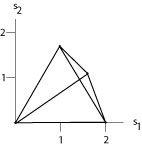
\includegraphics[height=2in]{2_tetra}}
\caption{Mapped tetrahedron of Solution \ref{op1_34}. \label{fig_tetra}}
\end{figure}

%%%%%%%%%%%%%%%%%%%%%%%%%%%%%%%%%%%%%%%%%%%%%%%%%%%%%%%%%%%%%%%%%%%%%%%%%%%%%%%%
\vspace{2mm}
\noindent {\bf Solution \ref{op1_35}}
We can write
\[
[s_1,s_2] = {{1}\over{\eee_3\cdot(\xx_0-\pp)+t\eee_3\cdot\vv}}[\eee_1\cdot(\xx_0-\pp)+t\eee_1\cdot\vv,\eee_2\cdot(\xx_0-\pp)+t\eee_2\cdot\vv]
\]
This means that $as_1+bs_2=c$ can be rewritten
\[
a(\eee_1\cdot(\xx_0-\pp)+t\eee_1\cdot\vv) + b(\eee_2\cdot(\xx_0-\pp)+t\eee_2\cdot\vv) - c(\eee_3\cdot(\xx_0-\pp)+t\eee_3\cdot\vv) = 0
\]
This holds for every $t$ if both these equations hold:
\[\matrix{
a(\eee_1\cdot(\xx_0-\pp)) &+ b(\eee_2\cdot(\xx_0-\pp)) &- c(\eee_3\cdot(\xx_0-\pp)) &= 0\cr
a\eee_1\cdot\vv &+ b\eee_2\cdot\vv &- c\eee_3\cdot\vv &=0\cr
}
\]
This is a system of two equations in three unknowns, $a$, $b$, and $c$. Such a system always has a non trivial solution (as we will see in
the following chapter.)

%%%%%%%%%%%%%%%%%%%%%%%%%%%%%%%%%%%%%%%%%%%%%%%%%%%%%%%%%%%%%%%%%%%%%%%%%%%%%%%%
\vspace{2mm}
\noindent {\bf Solution \ref{op1_36}}
In this case we want $\yy-\xx$ to point in the same direction as $\eee_3$ so
$\yy-\xx=\lambda\eee_3$. On the other hand $\yy$ lies on the plane of the
screen, so $\yy=\qq+s_1\eee_1+s_2\eee_2$. Therefore
\[
\qq-\xx+s_1\eee_1+s_2\eee_2=\lambda\eee_3.
\]
Now to find $s_1$ and $s_2$ take dot products with $\eee_1$ and $\eee_2$. This
yields
$s_1=-\eee_1\cdot(\qq-\xx)$ and $s_2=-\eee_2\cdot(\qq-\xx)$.


% \end{document}

\chapter{Solving Linear Systems}
\label{ch:ch3}

\section{Linear Systems}

\subsection{General Form of Linear Systems}

So far, we have seen systems of linear equations as the equations that
describe points, lines and planes. However, linear systems of
equations show up in many other ways in engineering problems. We will
solve linear systems to find the behaviour of an electrical circuit. 
Other examples
would be the calculation of equilibrium temperature distributions or
electric fields. Such examples often involve the discretization of a
continuous function. In other words, a continuous function like the
temperature distribution in a body (which has a value for each of the
infinitely many points in the body) will be replaced by a list of
temperatures at a large but finite number $n$ of closely spaced
points. This gives rise to a system of linear equations in $n$
unknowns, where $n$ can be in the tens of thousands, or
higher. Therefore, we want to develop a technique to solve systems of
linear equations in $n$ unknowns when $n$ is large.

The most general form of a linear system of equations is
\[
\matrix{
a_{1,1}x_1  &+&a_{1,2}x_2   &+\cdots    &+&a_{1,n}x_n   &= &c_1\cr
a_{2,1}x_1  &+&a_{2,2}x_2   &+\cdots    &+&a_{2,n}x_n   &= &c_2\cr
\vdots      &\vdots&        &   &&\vdots        &&\vdots\cr
a_{m,1}x_1  &+&a_{m,2}x_2   &+\cdots    &+&a_{m,n}x_n   &= &c_m\cr
}
\]
Here the numbers $a_{i,j}$ and $c_j$ are known, and the goal is to find
all values of $x_1,\ldots ,x_n$ that satisfy all the equations.

\subsection{Solving Linear Systems by Substitution}

Let us start with an example, which we will solve using the method of
{\em substitution}.
\begin{example}
\label{ex_substitution}
Consider the system of equations
\[\matrix{
x_1&+&x_2&+&x_3&=&6\cr
x_1&-&x_2&+&x_3&=&0\cr
2x_1&+&x_2&-&8x_3&=&-11\cr
}
\]
{\rm One could try to proceed as follows. Solve the first equations
for, say, $x_3$. This gives
\[
x_3=6-x_1-x_2.
\]
Now substitute this value for $x_3$ into the second and third equations.
This gives
\[
\matrix{
x_1&-&x_2&+&(6-x_1-x_2)&=&0\cr
2x_1&+&x_2&-&8(6-x_1-x_2)&=&-11\cr
}
\]
or
\begin{eqnarray*}
-2x_2 &=& -6 \\
10x_1+9x_2 &=& 37
\end{eqnarray*}
Now solve the first of these equations for $x_2$ and substitute into
the last equation. This gives $x_2=3$ and $x_1=1$. Finally we can go
back and calculate $x_3=6-1-3=2$.}
\end{example}

Although this procedure works fine for $n=2$ or even $n=3$, it rapidly
becomes unwieldy for larger values of $n$. We will now introduce a
technique called Gaussian elimination that works well for large $n$
and can be easily implemented on a computer.

We have already observed that there may be many systems of equations
with the same solution. When there are only two unknowns, this amounts
to saying that different pairs of lines may intersect in the same
point.  Gaussian elimination is based on the following idea.  We
introduce three elementary row operations. These operations change the
system of the equations into another system with exactly the same the
set of solutions. We then apply these elementary row operations in a
systematic way to change the system of equations into a system that is
easily solved.

\subsection{Elementary row (equation) operations}

The first elementary row operation is

\vspace{2mm}
\noindent {\em 1. Multiplication of a row (equation) by a non-zero number}
\vspace{2mm}

For example, if we multiply the first equation in the system of
Example~\ref{ex_substitution} above by $3$, we end up with
\[
\matrix{
3x_1&+&3x_2&+&3x_3&=&18\cr
x_1&-&x_2&+&x_3&=&0\cr
2x_1&+&x_2&-&8x_3&=&-11\cr
}
\]
This new system of equations has exactly the same solutions as the
original system, because we can undo the elementary row operation
simply by dividing the first equation by $3$. Thus the values
$x_1,x_2,x_3$ solve this system if and only if they solve the original
system. (Notice that this would not be true if we multiplied by
zero. In that case we could not undo the operation, and the new system
of equations could well have more solutions than the original system.)
Any row operations we do can be undone by other row operations, and 
the set of solutions of the linear system remain unchanged. 

The second elementary row operation is

\vspace{2mm}
\noindent {\em 2. Adding a multiple of one row (equation) to another row}
\vspace{2mm}

For example, if we added $2$ times the first row to the second row in our
example we would obtain the system
\[
\matrix{
x_1 &+&x_2  &+&x_3&=&6\cr
3x_1    &+&x_2  &+&3x_3&=&12\cr
2x_1&+&x_2&-&8x_3&=&-11\cr
}
\]
Again, the new system of equations has exactly the same solutions as
the original system, since we could undo this elementary row operation
by subtracting $2$ times the first row from the second row.

The third and final elementary row operation is

\vspace{2mm}
\noindent {\em 3. Interchanging two rows (equations)}
\vspace{2mm}

For example, if we swapped the first and second equations in our
original system we would end up with
\[
\matrix{
x_1&-&x_2&+&x_3&=&0\cr
x_1&+&x_2&+&x_3&=&6\cr
2x_1&+&x_2&-&8x_3&=&-11\cr
}
\]
This obviously doesn't change the solutions of the system since we have 
the same equalities. 

\subsection{Augmented Matrices}

To save unnecessary writing, we now set up an streamlined notation for
systems of linear equations. Notice that the only thing that
distinguished one system of equations from another are the
coefficients. So, as shorthand, we can write the system of equations
of Example~\ref{ex_substitution}
\[
\matrix{
x_1&+&x_2&+&x_3&=&3\cr
x_1&-&x_2&+&x_3&=&3\cr
2x_1&+&x_2&-&8x_3&=&-4\cr
}
\]
simply as
\[
\left[\matrix{
1&  1&  1\cr
1&  -1& 1\cr
2&  1&  -8\cr
}\right|\left. \matrix{
3\cr
3\cr
-4\cr
}\right]
\]
This is called an augmented matrix. ``Augmented'' refers to the column
to the right of the line that contains the information about the right
side of each equation.

\subsection{Problems}

\begin{problem}
\label{2009_a3_5}
Express the system
\[\begin{array}{rrrrrrr}
x_1 & - & 2x_2& + &3 x_3 &= &6 \\
4x_1 &- &5x_2&- &6x_3 &= &7\\
8x_1 &+&9x_2&+ &10x_3 &=&11
\end{array}\]
as an augmented matrix. 
\end{problem}

\begin{problem}
\label{op2_1}
Start with the system
\[
\matrix{
x_1&+&x_2&+&x_3&=&6\cr
x_1&-&x_2&+&x_3&=&0\cr
2x_1&+&x_2&-&8x_3&=&-11\cr
}
\]
and perform the following sequence of row operations:
\begin{enumerate}[1.]
\item Subtract the first row from the second row\par
\item Subtract twice the first row from the third row\par
\item Multiply the second row by $-1/2$\par
\item Add the second row to the third row\par
\item Multiply the third row by $-1/10$\par
Solve the  resulting system of equations by starting with the third
equation, then the second and then the first.
\end{enumerate}
\end{problem}

\begin{problem}
\label{matlab_op2_1}
(Matlab) Let's try to solve problem \ref{op2_1} using Matlab.

\begin{enumerate}[1.]
\item Start by generating an extended matrix to represent the system of equations:
\begin{verbatim}
A=[1, 1, 1, 6; 1, -1, 1, 0; 2, 1, -8, -11]
\end{verbatim}
\item Subtract the first row from the second row:
\begin{verbatim}
 A(2,:)=A(2,:)-A(1,:)
\end{verbatim}
\item Subtract twice the first row from the third row:
\begin{verbatim}
 A(3,:)=A(3,:)-2*A(1,:)
\end{verbatim}
\item Multiply the second row by $-1/2$:
\begin{verbatim}
 A(2,:)=-A(2,:)/2 
\end{verbatim}
\item etc.\par
% \item Add the second row to the third row\par
% \begin{verbatim}
%   A(3,:)=A(3,:)+A(2,:)
% \end{verbatim}
% \item Multiply the third row by $-1/10$\par
% \begin{verbatim}
%   A(3,:)=-A(3,:)/10
% \end{verbatim}

\end{enumerate}
What other commands are necessary to arrive at the solution? Does it coincide with the paper and pen solution?
\end{problem}

\begin{problem}
\label{2009_a3_4}
Start with the system
\[\begin{array}{rrrrrrr}
x_1 & - & x_2& + & x_3 &= &10 \\
x_1 &- &x_2&- &x_3 &= &6\\
6x_1 &+&3x_2&+ &x_3 &=&0
\end{array}
\]
Perform the following sequence of row operations
\\1. Subtract the second row from the first row
\\2. Add the first row to the second row
\\3. Subtract the first row from the third row
\\4. Multiply the second row by 3
\\5. Add the second row to the third row
\\Show that the resulting system of equations can be easily solved and find the solution of the above system of equations. 
\end{problem}

\begin{problem}
\label{2009_a3_3}
Without using the calculator or computer, find the solution to the system
\[\begin{array}{rrrrr}
2x_1 &+ &x_2 &= &5\\
3 x_1&+ &5 x_2 &= &-10
\end{array}\]
You can leave the solutions as fractions. 
\end{problem}

\section{Gaussian Elimination}

Recall that we want to use a sequence of elementary row operations to turn
an arbitrary system of equations into an easily solved system of equations
(with exactly the same solutions). What equations are easily solved?
Well, the easiest possible equations to solve are ones of the form
below, written as an augmented matrix:
\[
\left[\matrix{
1&  0&  0\cr
0&  1&  0\cr
0&  0&  1\cr
}\right|\left .\matrix{
3\cr
3\cr
-4\cr
}\right]
\]
If we translate from the shorthand back to the equations they
represent, the first row says $x_1=3$, the second row says $x_2=3$ and
the third row says $x_3=-4$. In other words, we can just read off the
values of $x_1$, $x_2$ and $x_3$ in the rightmost column. The
equations are already solved, and there is nothing left to do!

Slightly more work, but still easy to do, are upper triangular
systems. These are systems where all the entries below the diagonal
are equal to zero, as in
\[
\left[\matrix{
1&  1&  1\cr
0&  -1& 1\cr
0&  0&  -4\cr
}\right|\left .\matrix{
3\cr
3\cr
-8\cr
}\right]
\]
The reason these are easy to solve is that the equation represented by
the $j$th row only involves the variables $x_j, x_{j+1},\ldots,
x_n$. So if we start with the last equation (in the example
$-4x_3=-8$), we can solve it immediately for $x_n$ (in the example
$x_3=2$). Now we move up one equation. This equation only involves
$x_{n-1}$ and $x_n$, and we already know $x_n$. So we can solve it for
$x_{n-1}$ (in the example $-x_2+x_3=3$ so $-x_2+2=3$ so $x_2=-1$).  We
can continue in this way until all the $x_n$'s have been found. (In
the example there is one more equation $x_1+x_2+x_3=3$ or $x_1-1+2=3$
or $x_1=2$.)

In practise (i.e., in a typical computer program) the procedure that
is actually used is to apply a sequence of row operations to turn the
system of equations into an upper triangular system. Then the
equations are solved one by one, starting at the bottom and working
up. This is the most efficient way to solve a system of
equations. However, its sometimes convenient to apply row operations
to bring the equation into the ``completely solved'' form. Then, you
can just read off the solution from the last column.

Let us now do a bunch of examples to illustrate this procedure. I'll
cook them up so that everything that possibly can go wrong, does go
wrong. (I'll also cook them up so that the numbers come out looking
nice. This will definitely not be the case in an example coming up in
a real application!). Here is a shorthand for indicating which
elementary row operation was done. The notation $3(1,:)$ means the first
row was multiplied by the non-zero number $3$. The notation $(2,:)=(2,:)-4(5,:)$
means that $4$ times the fifth row was subtracted from the second
row. Finally, $(2,:)\leftrightarrow (3,:)$ means that the second and third
row were interchanged.

\begin{example} \label{ex_gebs} Let us start with
\[
\left[
\begin{array}{cccc}
1&2&-2&-7 \\
1&2&-1&-5 \\
0&3&0&-3 \\
-1&4&1&1
\end{array} \right| \left.
\begin{array}{c}
-29 \\ -18 \\ -6 \\ 14 
\end{array}
\right]
\]
{\rm We are trying to put this matrix in upper triangular form. So we start by
trying to produce zero entries in the first column under the top entry. We
can do this by adding multiples of the first row to the other rows. So, the
first move is to subtract the first row from the second row. The
result is
\[
\left[
\begin{array}{cccc}
1&2&-2&-7 \\
0&0&1&2 \\
0&3&0&-3 \\
-1&4&1&1
\end{array} \right| \left.
\begin{array}{c}
-29 \\ 11 \\ -6 \\ 14 
\end{array}
\right]
\begin{array}{c} 
 \\ (2,:)=(2,:)-(1,:) \\ \\ \hfill
\end{array}
\]
The third row already has a zero in the first column, so there is nothing to
do here. To put a zero in the fourth row we add the first row to the
last row.
\[
\left[
\begin{array}{cccc}
1&2&-2&-7 \\
0&0&1&2 \\
0&3&0&-3 \\
0&6&-1&-6
\end{array} \right| \left.
\begin{array}{c}
-29 \\ 11 \\ -6 \\ -15 
\end{array}
\right]
\begin{array}{c} 
 \\ \\ \\ (4,:)=(4,:) +(1,:)
\end{array}
\]
Now we shift our attention to the second column. We want to produce
zeros below the diagonal. If we attempt to do this by adding multiples
of the first row to other rows, we will destroy the zeros that we have
already produced. So we try to use the second row. This is where we
run into the first glitch. Since the entry in the second column of the second row
is zero, adding a multiple of this row to the others won't have any
effect on the numbers in the second column that we are trying to
change. To remedy this we simply swap the second and third rows.
\[
\left[
\begin{array}{cccc}
1&2&-2&-7 \\
0&3&0&-3 \\
0&0&1&2 \\
0&6&-1&-6
\end{array} \right| \left.
\begin{array}{c}
-29 \\ -6 \\ 11 \\ -15 
\end{array}
\right]
\begin{array}{c} 
 \\(2,:)\leftrightarrow(3,:)\\ \hfill
\end{array}
\]
Now we can complete the job on the second column by subtracting $2$
times the second row from the last row.
\[
\left[
\begin{array}{cccc}
1&2&-2&-7 \\
0&3&0&-3 \\
0&0&1&2 \\
0&0&-1&0
\end{array} \right| \left.
\begin{array}{c}
-29 \\ -6 \\ 11 \\ -3 
\end{array}
\right]
\begin{array}{c} 
 \\ \\ \\ (4,:)=(4,:)-2(2,:) \hfill
\end{array}
\]
Now we shift our attention to the third column. To produce a zero in the
entry below the diagonal we must add the third row to the last row.
\[
\left[
\begin{array}{cccc}
1&2&-2&-7 \\
0&3&0&-3 \\
0&0&1&2 \\
0&0&0&2
\end{array} \right| \left.
\begin{array}{c}
-29 \\ -6 \\ 11 \\ 8 
\end{array}
\right]
\begin{array}{c} 
 \\ \\ \\ (4,:)=(4,:)+(3,:)
\end{array}
\]
The matrix is now in upper triangular form. Let us find the
solution. This last row is shorthand for the equation $2x_4=8$. So
$x_4=2$. The third row now gives $x_3+2(4)=11$, so $x_3=3$. The second
row gives $3x_2 - 3(4)=-6$ so $x_2=2$. Finally the first row gives
$x_1+2(2)-2(3)-7(4)=-29$ so $x_1=1$.}
\end{example}

\begin{example} 
\label{ex_rref}
There is really no need to do anything more in
Example~\ref{ex_gebs}, but let us  continue with elementary
row operations to put the equations into the ``completely solved'' form,
just to see how this goes. {\rm First we divide the second row by $3$.
\[
\left[
\begin{array}{cccc}
1&2&-2&-7 \\
0&1&0&-1 \\
0&0&1&2 \\
0&0&0&2
\end{array} \right| \left.
\begin{array}{c}
-29 \\ -2 \\ 11 \\ 8 
\end{array}
\right]
\begin{array}{c} 
 \\(2,:)=(1/3)(2,:) \\ \\ \hfill
\end{array}
\]
Now we subtract twice the second row from the first row.
\[
\left[
\begin{array}{cccc}
1&0&-2&-5 \\
0&1&0&-1 \\
0&0&1&2 \\
0&0&0&2
\end{array} \right| \left.
\begin{array}{c}
-25 \\ -2 \\ 11 \\ 8 
\end{array}
\right]
\begin{array}{c} 
(1,:)=(1,:)-2(2,:) \\ \\ \\ \hfill
\end{array}
\]
Now add twice the third row to the first row. Then divide the last row
by $2$.
\[
\left[
\begin{array}{cccc}
1&0&0&-1 \\
0&1&0&-1 \\
0&0&1&2 \\
0&0&0&1
\end{array} \right| \left.
\begin{array}{c}
-3 \\ -2 \\ 11 \\ 4 
\end{array}
\right]
\begin{array}{c} 
(1,:)=(1,:)+2(3,:) \\ \\ \\ (4,:)=(1/2)(4,:)
\end{array}
\]
Finally, we add various multiples of the last row to the previous rows.
\[
\left[
\begin{array}{cccc}
1&0&0&0 \\
0&1&0&0 \\
0&0&1&0 \\
0&0&0&1
\end{array} \right| \left.
\begin{array}{c}
1 \\ 2 \\ 3 \\ 4 
\end{array}
\right]
\begin{array}{c} 
(1,:)=(1,:)+(4,:) \\ (2,:)=(2,:)+(4,:) \\ (3,:)=(3,:)-2(4,:) \\ \hfill
\end{array}
\]
We now can read the solution off from the last column.}
\end{example}

In the previous example there was a unique solution to the system of
equations.  We already know, from the geometrical meaning of the
equations, that sometimes there will be lots of solutions depending on
a parameter.  This is expected to happen when there are fewer
equations than unknowns (e.g., the intersections of two planes in
three dimensional space is usually a line) but will also occur in
certain degenerate cases when the number of equations is equal to or
more than the number of unknowns (e.g., three, or even four, planes may
intersect in a line too). What happens in the procedure of row
reductions when there are parameters in the solution? Let us  look at
another example.

\begin{example} Consider the system 
\[
\left[
\begin{array}{cccc}
1&3&2&-2 \\
1&3&4&-2 \\
-2&-6&-4&5 \\
-1&-3&2&1
\end{array} \right| \left.
\begin{array}{c}
-1 \\ 3 \\ 5 \\ 6 
\end{array}
\right]
\]
Perform Gaussian Elimination on this system. {\rm We begin, as before,
by trying to produce zeros in the first column under the diagonal
entry. This procedure yields
\[
\left[
\begin{array}{cccc}
1&3&2&-2 \\
0&0&2&0 \\
0&0&0&1 \\
0&0&4&-1
\end{array} \right| \left.
\begin{array}{c}
-1 \\ 4 \\ 3 \\ 5 
\end{array}
\right]
\begin{array}{c} 
 \\(2,:)=(2,:)-(1,:) \\(3,:)=(3,:)+2(1,:)  \\ (4,:)=(4,:)+(1,:)
\end{array}
\]
As in the previous example, there is now a zero sitting in the
diagonal spot in the second column. Last time, we swapped rows at this
point to put a non-zero entry in this place. But now, all the other
entries below this one are zero too! So there is nothing we can swap
in to save the situation. (Clearly, swapping the first row down is not
a good idea, since that would destroy the zero in the first column.)
So we just have to admit defeat, and shift our attention one column to
the right. We subtract twice the second row from the fourth row.
\[
\left[
\begin{array}{cccc}
1&3&2&-2 \\
0&0&2&0 \\
0&0&0&1 \\
0&0&0&-1
\end{array} \right| \left.
\begin{array}{c}
-1 \\ 4 \\ 3 \\ -3 
\end{array}
\right]
\begin{array}{c} 
 \\ \\ \\ (4,:)=(4,:)-2(2,:)
\end{array}
\]
Now we complete the job by adding the third row to the last row.
\[
\left[
\begin{array}{cccc}
1&3&2&-2 \\
0&0&2&0 \\
0&0&0&1 \\
0&0&0&0
\end{array} \right| \left.
\begin{array}{c}
-1 \\ 4 \\ 3 \\ 0 
\end{array}
\right]
\begin{array}{c} 
 \\ \\ \\ (4,:)=(4,:)+(3,:)
\end{array}
\]
What are the solutions? The third equation says $x_4=3$ and the second
equation says $x_3=2$. There is nothing new here. However the first
equation introduces not just one, but two new variables $x_1$ and
$x_2$.  It reads $x_1+3x_2+2(2)-2(3)=-1$, or, $x_1+3x_2=1$ Clearly,
there are infinitely many values of $x_1$ and $x_2$ that satisfy this
equation. In fact, if we fix $x_2$ to be any arbitrary value $x_2=s$,
and then set $x_1=1-3s$, $x_1$ and $x_2$ will be solutions.  So for
any choice of $s$
\[
x_1=1-3s, x_2=s, x_3=2, x_4=3
\]
is a solution. There are infinitely many solutions depending on a
parameter $s$.  We could also write this as
\[
\left[\matrix{x_1\cr x_2\cr x_3\cr x_4\cr}\right]=
\left[\matrix{1\cr 0\cr 2\cr 3\cr}\right]
+ s\left[\matrix{-3\cr 1\cr 0\cr 0\cr}\right]
\]
and recognize the solutions as a line in four dimensional space
passing through $[1,0,2,3]$ in the direction $[-3,1,0,0]$.}
\end{example}

There is one situation left to consider, namely when there are no solutions
at all. Geometrically, this happens, for example, when we are trying to
find the intersection of two parallel planes. Let us  look at an example.

\begin{example} Perform Gaussian Elimination on the following system
\[
\left[
\begin{array}{cc}
1&3 \\
1&4 \\
-1&-3\\
2&6 
\end{array} \right| \left.
\begin{array}{c}
1 \\ 2 \\ 0 \\ 4 
\end{array}
\right]
\]
{ \rm We begin in the usual way.
\[
\left[
\begin{array}{cc}
1&3 \\
0&1 \\
0&0\\
0&0 
\end{array} \right| \left.
\begin{array}{c}
1 \\ 1 \\ 1 \\ 2 
\end{array}
\right]
\begin{array}{c} 
 \\ (2,:)=(2,:)-(1,:) \\ (3,:)=(3,:)+(1,:) \\ (4,:)=(4,:)-2(1,:)
\end{array}
\]
There is nothing left to do in the second column,
so we shift our attention to the third column and subtract twice the third row
from the fourth row.
\[
\left[
\begin{array}{cc}
1&3 \\
0&1 \\
0&0\\
0&0
\end{array} \right| \left.
\begin{array}{c}
1 \\ 1 \\ 1 \\ 0
\end{array}
\right]
\begin{array}{c}
 \\ \\ \\ (4,:)=(4,:)-2(3,:)
\end{array}
\]
Now we are done. If we write
down the equation corresponding to the third row, we get
$0x_1+0x_2=1$, or $0=1$. Clearly there is no choice of $x_1$ or $x_2$ that
makes this true. So this is a system
of equations with no solutions.}
\end{example}

Let us  summarize what we have done in this section. Every system of equations
can be brought into upper triangular form using a sequence of elementary row
transformations. The resulting upper triangular matrix will look something like
what is shown in Figure~\ref{fig_hermite1} (left).
In this diagram, all the entries below the staircase line are zero. The boxes
represent non-zero entries. The stars represent arbitrary entries, that may or
may not be zero. Each circled star corresponds to a parameter that must be
introduced.

\begin{figure}
\centerline{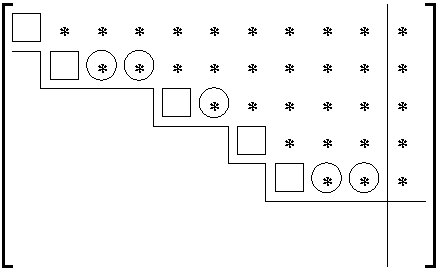
\includegraphics[height=1.25in]{3_hermite1}
\hspace{5mm}
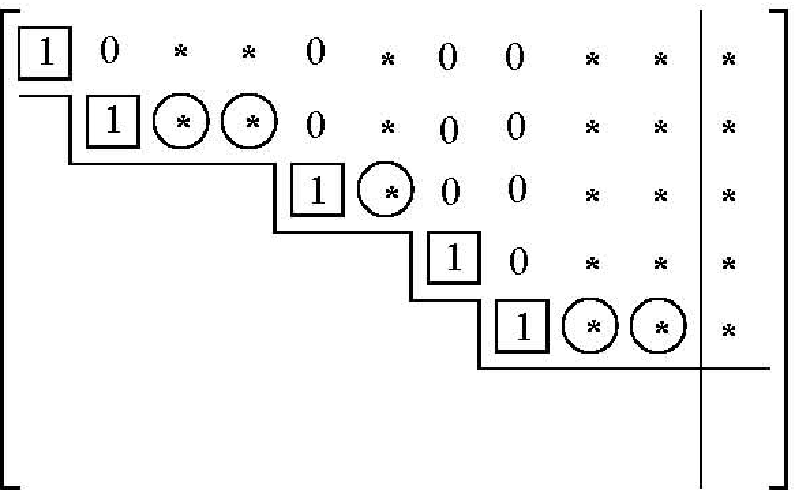
\includegraphics[height=1.25in]{3_hermite1rref}}
\caption{After Gaussian Elimination the augmented matrix will be 
in row echelon form (left). With further work, the augmented matrix can 
be put in reduced row echelon form (right). 
\label{fig_hermite1}}
\end{figure}

If we want to put this example in completely reduced form, we
use elementary row operations to zero out the entries
lying above the boxes too. Then we
multiply each row by a number so that the corner entries (in the boxes)
become $1$. The completely reduced form for the example above 
would look like the diagram in Figure~\ref{fig_hermite1} (right). 
The official name of this form is the {\em reduced row echelon form}.

If the bottom of the matrix has a row that is all zeroes, except for the
augmented entry, then the system of equations has no solutions. This is because
the bottom row stands for an equation of the form $0=\Box$ with $\Box\ne 0$.
A typical example is shown in Figure~\ref{fig_hermite2} (left). 

\begin{figure}
\centerline{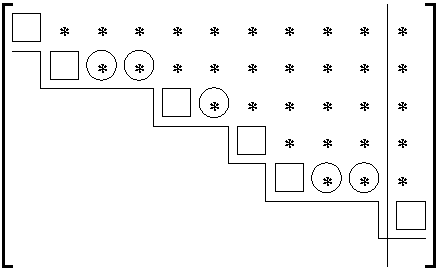
\includegraphics[height=1.5in]{3_hermite2}
\hspace{5mm}
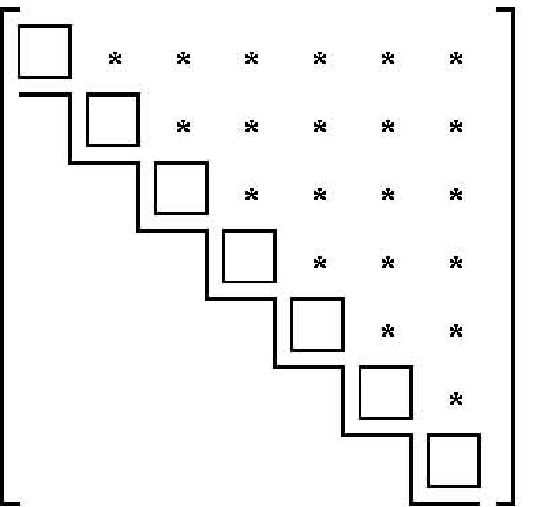
\includegraphics[height=1.5in]{3_hermite3}}
\caption{Augmented matrices after Gaussian Elimination 
with no solutions (left) and with a single solution (right). 
\label{fig_hermite2}}
\end{figure}

If all the steps on the staircase in the non-augmented part of the matrix
have size one, then there are no parameters to introduce, and the solution is
unique. Notice that in this case there are the same number of equations as
variables. A typical example is shown in Figure~\ref{fig_hermite2} (right). 

Finally, we introduce some terminology.
The {\it rank} of a matrix is the number of non-zero rows in the matrix obtained
after reducing it to the upper triangular form described above. In other words
the rank is the number of boxes in the diagrams above. We can now rephrase the
different possibilities in terms of rank. If the rank of the augmented matrix is
greater than the rank of the unaugmented matrix (i.e., the matrix without the
last column) then there are no solutions. If the rank of the matrix is equal
to the number of unknowns then the solution is unique. If the rank $r$ of the matrix
is equal to the rank of the unaugmented matrix, but less than the number $n$ of
unknowns, then there are $n-r$ parameters in the solution.

Ordinary arithmetic errors are a common source of errors when you do row operations
by hand. There is a technique called ``the check column'' that can often catch such errors. It is described in Section~\ref{s:check}. Another easy way to make sure that we have not made any mechanical errors in calculating the solution of a linear system is just to substitute the purported solution
back into the original system and verify that each left hand side really is equal to its corresponding
right hand side.

\subsection{Using MATLAB for row reductions}

MATLAB has a built in command
called {\tt rref} that reduces a matrix to reduced row echelon form.
Let us  try it on the example in the previous section. First we define
the initial matrix {\tt A}. Remember that the last column of this matrix is
the augmented part.
\begin{verbatim} 
A = [1 2 -2 -7 -29; 1 2 -1 -5 -18; 0 3 0 -3 -6; -1 4 1 1 14]
\end{verbatim}
To find the reduced row echelon form, simply type
\begin{verbatim}
>> rref(A)
ans = 
1 0 0 0 1
0 1 0 0 2
0 0 1 0 3
0 0 0 1 4
\end{verbatim}
Notice that this MATLAB command did the work of Examples~\ref{ex_gebs} 
and~\ref{ex_rref}. The solution to the system can be read off the result
of the {\tt rref} command above. 

It is important to realize that floating point rounding errors as discussed in 
Section~\ref{sec:floating} can lead to errors in solutions to linear systems computed 
by MATLAB and other computational tools. At worst, these errors will lead to MATLAB 
finding ``solutions'' to problems that do not have exact solutions. In these cases, 
solutions will often have very large values and often MATLAB will give a warning 
about the problem being ``ill-conditioned".   

\subsection{Problems}

\begin{problem}
\label{op2_2}
Show that the lower triangular system of equations represented by
\[
\left[\matrix{
1&  0&  0\cr
1&  -1& 0\cr
2&  1&  -8\cr
}\right|\left .\matrix{
3\cr
3\cr
-4\cr
}\right]
\]
is also easily solved, by easily solving it! It's just a matter of convention
whether we aim for upper triangular or lower triangular systems in the
elimination procedure.
\end{problem}

\begin{problem}
\label{op2_3}
The following equations have already
been put in upper triangular form. In each case there are infinitely
many solutions, depending on one or more parameters.  Write down the
general expression for the solution in terms of parameters.
\[
\left[
\begin{array}{cccc}
1&2&1&2 \\
0&0&1&1 \\
0&0&0&1 \\
0&0&0&0 \\
\end{array} \right| \left.
\begin{array}{c}
1 \\ 4 \\ 2 \\ 0
\end{array}
\right]
\]

\[
\left[
\begin{array}{cccc}
1&2&1&2 \\
0&0&1&1 \\
0&0&0&0 \\
0&0&0&0 
\end{array} \right| \left.
\begin{array}{c}
1 \\ 4 \\ 0 \\ 0
\end{array}
\right]
\]

\[
\left[\matrix{
1&2&1&2\cr
0&0&1&1\cr
}\right.\left|\matrix{
1\cr 4\cr
}\right]
\]
\end{problem}

\begin{problem}
\label{2009_a4_3}
Consider the system of equations represented by the augmented matrix
\[
\left[
\begin{array}{c c c c | c}
1 & 2 &2 & 2 & 1\\
1 & 3& -1&3 & -1\\
1&0 &1 &1 & 5 \\
0& 3 & -2 & 2 & -6
\end{array}
\right]
\]
Show that this set of equations has infinitely many solutions and find a general parametric representation of the solutions.
\end{problem}

\begin{problem}
\label{2009_a4_1}
Consider the system of equations represented by the augmented matrix
\[
\left[
\begin{array}{c c c c | c}
1 & 2 &2 & -7 & 20\\
3 & 6& -3&-5 &-15\\
0&6 &0 &-6 & -10 \\
2& -8 & -2 & -2 & 30
\end{array}
\right]
\]
Put this matrix in upper triangular form and find the solution of the linear system of equations. You can leave your answers in fractions but show the operations you perform in full detail. 
\end{problem}

\begin{problem}
\label{op2_4}
Solve the following system of equations.
\[
\matrix{
x_1 &-& 2x_2 &+& 3x_3 &=& 2\cr
2x_1 &-& 3x_2 &+& 2x_3 &=& 2\cr
3x_1 &+& 2x_2 &-& 4x_3 &=& 9\cr
}
\]
\end{problem}

\begin{problem}
\label{op2_5}
Solve the following system of equations.
\[
\matrix{
2x_1 &+& x_2 &-& 1x_3 &=& 6\cr
x_1 &-& 2x_2 &-& 2x_3 &=& 1\cr
-x_1 &+& 12x_2 &+& 8x_3 &=& 7\cr
}
\]
\end{problem}

\begin{problem}
\label{op2_6}
Solve the following system of equations.
\[
\matrix{
x_1 &+& 2x_2 &+& 4x_3 &=& 1\cr
x_1 &+& x_2 &+& 3x_3 &=& 2\cr
2x_1 &+& 5x_2 &+& 9x_3 &=& 1\cr
}
\]
\end{problem}

\begin{problem}
\label{op2_7}
Solve the following system of equations.
\[
\matrix{
x_1 &+& 2x_2 &+& 4x_3 &=& 1\cr
x_1 &+& x_2 &+& 3x_3 &=& 2\cr
2x_1 &+& 5x_2 &+& 9x_3 &=& 3\cr
}
\]
\end{problem}

\begin{problem}
\label{op2_8}
Solve the following system of equations.
\[
\matrix{
3x_1 &+& x_2 &-& x_3 &+& 2x_4 &=& 7\cr
2x_1 &-& 2x_2 &+& 5x_3 &-& 7x_4&=& 1\cr
-4x_1 &-& 4x_2 &+& 7x_3 &-& 11x_4&=& -13\cr
}
\]
\end{problem}

\begin{problem} 
\label{op2_9}
For what values of $a$, $b$, $c$, $d$, $\alpha$ and $\beta$ does
the system of equations
\[
\matrix{
ax_1 &+& bx_2 &=& \alpha\cr
cx_1 &+& dx_2 &=& \beta\cr
}
\]
have a unique solution?
\end{problem}

\begin{problem}
\label{2009_a4_2}
Consider the system of equations represented by the augmented matrix
\[
\left[
\begin{array}{c c c | c}
1 & 2 & 0 & 7\\
4 & 8 & 6 & 10\\
-4 & -8 & 10 & 81
\end{array}
\right]
\]
How many solutions does this linear system of equations have?
\end{problem}

\begin{problem}
\label{matlab_2009_a4_2}
(Matlab) Consider the following system of equations
\[
\matrix{
x_1 &+& 2x_2 &+& 4x_3 &=& 7\cr
4x_1 &+& x_2 &+& 3x_3 &=& 2\cr
0 &+& 5x_2 &+& 9x_3 &=& a\cr
}
\]
\end{problem}
Write a script in Matlab that generates the augmented matrix and solves the system with the {\tt rref} command for various values of $a$. Specifically, how does the solution of {\tt $x_1$} vary when you range $a$ from 1 to 10 (equally spaced)?

\section{Homogeneous Equations} 

If the coefficients on the right sides of a system of equations are all zero,
the system is said to be {\it homogeneous}. In other words, a homogeneous system
is a system of equations of the form
\[
\matrix{
b_{1,1}x_1      &+&b_{1,2}x_2   &+\cdots        &+&b_{1,n}x_n   &= &0\cr
b_{2,1}x_1      &+&b_{2,2}x_2   &+\cdots        &+&b_{2,n}x_n   &= &0\cr
\vdots          &\vdots&                &       &&\vdots                &&\vdots
\cr
b_{m,1}x_1      &+&b_{m,2}x_2   &+\cdots        &+&b_{m,n}x_n   &= &0\cr
}
\]
Given a system of equations, the {\it associated homogeneous system} is the
homogeneous system of equations you get by setting all the right sides to zero.

Geometrically, homogeneous systems describe points, lines and planes that pass through the origin. In fact $\xx=\zv$, i.e.,
$x_1=0, x_2=0, \ldots, x_n=0$ is always a solution to a homogeneous system of equations.

When are there {\em{other (nonzero)}} solutions to the above homogeneous system? We have $n$ unknowns and $m$ equations.
When we perform the Gaussian reduction, the right-hand sides of the equations will stay zero
so the augmented matrix will generally have the form
\[
\left[\matrix{ 1&  *&  *& *& \cdots&\cdots&\cdots&*\cr  0&  1&  *& *&  \cdots&\cdots&\cdots& *\cr 0&  0&  0& 1&  *
&\cdots&\cdots& *\cr  \cdots&\cdots&\cdots&\cdots&\cdots&\cdots&\cdots&\cdots\cr  0&  0&  0& \cdots&0& 1& *&  * \cr  0& 0&
0& \cdots& \cdots& \cdots &1&*\cr  0&  0&  0& \cdots&0& 0& 0&  1 \cr
\cdots&\cdots&\cdots&\cdots&\cdots&\cdots&\cdots&\cdots\cr 0&  0&  0& \cdots&0& 0& 0& 0\cr
  }\right|\left .\matrix{ 0\cr0\cr0\cr \cdots \cr0\cr0\cr 0\cr\cdots\cr 0\cr }\right].
\]
The last several lines may be identically zero. In the last section we saw
that there are solutions depending on parameters if the number of variables
is greater than the rank of the matrix. Thus,
if $n$ (the number of unknowns) is bigger
than the number of non-zero lines in the above row-reduced matrix, 
then there exists a non-zero solution. Otherwise only a
trivial solution $x_1=0, x_2=0, \ldots, x_n=0$ is present. 
We illustrate the idea with some examples below.

\begin{example}
Consider a homogeneous system
\[
\matrix{ 3x_1      &+& 6 x_2   &+&x_3   &= &0\cr 6x_1      &+& 2 x_2   &+&2 x_3   &= &0\cr x_1      &+&  x_2   &+&3 x_3 &=
&0\cr}
\]
{\rm The augmented matrix can be reduced by row operations to the form (check!)
\[
\left[\matrix{ 1&  0&  0\cr 0&  1&  0\cr 0&  0&  1\cr }\right|\left .\matrix{ 0\cr 0\cr 0\cr }\right],
\]
which implies $x_1=x_2=x_3=0$. And, in agreement with our above statement, the number of variables (3) is not more than the
number of non-zero rows (also 3).}
\end{example}

\begin{example}
Consider another homogeneous system:
\[
\matrix{ -x_1      &+& 2 x_2   &+&4x_3   &= &0\cr 2x_1      &-& 4 x_2   &-&8 x_3   &= &0\cr x_1      &-&  x_2   &+&3 x_3 &=
&0\cr}.
\]
{\rm Its augmented matrix is 
\[
\left[\matrix{ -1&  2&  4\cr 2&  -4&  -8\cr 1&  -1&  3\cr }\right|\left .\matrix{ 0\cr 0\cr 0\cr }\right] ~\rightarrow~
\left[\matrix{ -1& 2& 4\cr 0&  0&  0\cr 0&  1&  7\cr }\right|\left .\matrix{ 0\cr 0\cr 0\cr }\right]~\rightarrow~
\left[\matrix{ 1& 0& 10\cr 0&  1&  7\cr 0&  0&  0\cr }\right|\left .\matrix{ 0\cr 0\cr 0\cr }\right],
\]
and the number of nonzero rows is 2, which is less than the number of unknowns, 3. Hence by the above statement there must
be a nonzero solution. We find $x_1=-10x_3$, $x_2=-7x_3$, with no 
requirement on $x_3$. Hence $x_3$ is any number $t$, and we
obtain infinitely many nonzero solutions
\[
x_1=-10t, \mbox{\ \ } x_2=-7t, \mbox{\ \ } x_3=t,~~~~t\in (-\infty,\infty),
\]
one for each value of t.}
\end{example}

In a similar manner, if for some homogeneous system with 4 variables the augmented matrix has only 2 nonzero rows, then the
general solution has 4-2=2 free (undefined) variables on which the other two depend.

\subsection{Properties of solutions of homogeneous systems.}

\begin{enumerate}
\item A homogeneous system has either one zero-solution $(x_1=...=x_n=0)$ or infinitely-many solutions that depend on
parameters.
\item If $(x_1,...,x_n)$ and $(y_1,...,y_n)$ are solutions to a given homogeneous system, $(x_1+y_1,...,x_n+y_n)$ is
also a solution. (Solutions are additive.)
\item If $(x_1,...,x_n)$ is a solution to a given homogeneous system, $(ax_1,...,ax_n)$ is also a solution, for any
number $a$. (Solutions are scalable.)
\end{enumerate}

The first statement follows from our previous discussion; the other two are easy to verify, using the initial homogeneous
system.

\subsection{Connection of solutions to homogeneous and inhomogeneous systems.}

The importance of homogeneous equations comes from the following fact. If $\xx=[x_1,x_2,\ldots,x_n]$ and
$\yy=[y_1,y_2,\ldots,y_n]$ are two solutions to a (not necessarily homogeneous) system of equations,
\[
\matrix{
b_{1,1}x_1      &+&b_{1,2}x_2   &+\cdots        &+&b_{1,n}x_n   &= &c_1\cr
b_{2,1}x_1      &+&b_{2,2}x_2   &+\cdots        &+&b_{2,n}x_n   &= &c_2\cr
\vdots          &\vdots&                &       &&\vdots                &&\vdots
\cr
b_{m,1}x_1      &+&b_{m,2}x_2   &+\cdots        &+&b_{m,n}x_n   &= &c_m\cr
}
\]
then the difference
$\xx-\yy=[x_1-y_1,x_2-y_2,\ldots,x_n-y_n]$ solves the associated homogeneous
system. This is a simple calculation
\[
\matrix{
b_{1,1}(x_1-y_1)      &+&b_{1,2}(x_2-y_2)   &+\cdots        &+&b_{1,n}(x_n-y_n)
 &= &(c_1-c_1) &= &0\cr
b_{2,1}(x_1-y_1)      &+&b_{2,2}(x_2-y_2)   &+\cdots        &+&b_{2,n}(x_n-y_n)
 &= &(c_2-c_2) &= &0\cr
\vdots          &\vdots&                &       &&\vdots                &&\vdots
\cr
b_{m,1}(x_1-y_1)      &+&b_{m,2}(x_2-y_2)   &+\cdots        &+&b_{m,n}(x_n-y_n)
 &= &(c_m-c_m) &= &0\cr
}
\]
To see the implications of this let us  suppose that $\xx=\qq$ is any particular
solution to a (non-homogeneous) system of equations. Then if $\yy$ is any other
solution $\yy-\xx=\zz$ is a solution of the corresponding homogeneous system.
So $\yy=\qq+\zz$. In other words any solution can be written as $\qq +$ some
solution of the corresponding homogeneous system. Going the other way, if
$\zz$ is any solution of the corresponding homogeneous system, then $\qq+\zz$
solves the original system. This can be seen by plugging $\qq+\zz$ into the
equation. So the structure of the set of solutions is
\[
\xx = \qq + (\mbox{{\ \bf solution to homogeneous system}})
\]
As you run through all solutions to the homogeneous system on the right,
$\xx$ runs through all solutions of the original system. Notice that it doesn't
matter which $\qq$ you choose as the starting point. This is completely analogous
to the parametric form for a line, where the base point can be any
point on the line.

If we have applied the process of
Gaussian elimination to the original system, and concluded that
the general solution has  parameters, we will end up with a general solution of
the form
\[
\qq + s_1\aa_1+\cdots +s_n\aa_n.
\]
Notice that $\qq$ is a particular solution (corresponding to all parameters
equal to zero) and $s_1\aa_1+\cdots +s_n\aa_n$ is the general solution to the
corresponding homogeneous system.

These considerations have practical importance if you have to solve a bunch of
systems, all with the same coefficients on the left side, but with different
coefficients on the right. In this situation, you could first find the general
solution to the corresponding homogeneous system of equations. Then to find the
general solution to one of the systems, you would only need to find a single
particular solution, and then add the general solution to the homogeneous system
to obtain all solutions. The only trouble with this is that it might not really
be any easier to find a single particular solution than it is to find all
solutions.

\begin{example}
\label{op2_10}
Find the general solution of the system of equations
\[
\left[\matrix{
1&1&0&0\cr
-1&-1&1&2\cr
3&3&-1&-2\cr
}\right . \left |\matrix{
1\cr 1\cr 1\cr
}\right]
\]
In the form $\xx=\qq+s_1\aa_1+s_2\aa_2$. Verify that $\aa_1$ and $\aa_2$ solve
the corresponding homogeneous equation.
{\rm The matrix 
\[
\left[
\begin{array}{cccc}
1&1&0&0 \\
-1&-1&1&2 \\
3&3&-1&-2
\end{array} \right| \left.
\begin{array}{c}
1 \\ 1 \\ 1
\end{array}
\right]
\]
reduces to
\[
\left[
\begin{array}{cccc}
1&1&0&0 \\
0&0&1&2 \\
0&0&0&0
\end{array} \right| \left.
\begin{array}{c}
1 \\ 2 \\ 0
\end{array}
\right]
\]
so the solutions are
$x_1=1-s_1$, $x_2=s_1$, $x_3=2-2s_2$, $x_4=s_2$. This can be written
\[
\xx = \left[\matrix{1\cr 0\cr 2\cr 0\cr}\right] + s_1\left[\matrix{-1\cr 1\cr 0\cr 0\cr}\right]
+s_2\left[\matrix{0\cr 0\cr -2\cr 1\cr}\right] 
\]
It's easy to check that $\aa_1=[-1,1,0,0]$ and $\aa_2=[0,0,-2,1]$ solve the 
corresponding homogeneous system.}
\end{example}

\subsection{Problems} 

\begin{problem}
\label{2009_a4_4}
Find the general solution of the system of equations
\[
\left[
\begin{array}{c c c c | c}
1 & 0 &1 & 0 & 10\\
-1 & 1& 1&1 & 4\\
0&1 &2 &1 & 14
\end{array}
\right]
\]
In the form $ {\bf x} = {\bf q} + s_1 {\bf a}_1+ s_2 {\bf a}_2$, where ${\bf a_1}$ and ${\bf a}_2$ solve the corresponding homogeneous system of equations. 
\end{problem}

\begin{problem}
\label{op2_11}
Consider the system of equations
\[
\left[\matrix{
1&1&0&0\cr
-1&-1&1&2\cr
3&3&-1&-2\cr
}\right . \left |\matrix{
4\cr -1\cr 9\cr
}\right]
\]
Verify that $[4,0,3,0]$ is a solution and write down the general solution.
\end{problem}

\begin{problem}
\label{2009_a4_5}
Consider the system of equations given by the augmented matrix
\[
\left[
\begin{array}{c c c  | c}
1 & -3 &4 & 6 \\
1 & 9& -10&10 \\
0&6 &-7 &2
\end{array}
\right]
\]
Put this matrix in reduced row echelon form and comment on the number of solutions of this system of equations. 
\end{problem}

\section{Geometric Applications}
\label{s:geom}

Now we will apply Gaussian elimination to some of the geometry problems
we studied in the first part of this course. 

Let us start with the question of linear independence. Recall that a collection
of vectors $\xx_1, \xx_2, \ldots, \xx_n$ is called linearly dependent if
we can find some non-zero coefficients $c_1, c_2, \ldots, c_n$ such that
\[
c_1\xx_1 + c_2\xx_2 + \cdots + c_n\xx_n = \zv
\]
This is actually a homogeneous system of linear equations for the numbers
$c_1, \ldots, c_n$. If $c_1=c_2=\cdots =c_n=0$ is the only solution, then
the vectors are linearly independent. Otherwise, they are linearly dependent.
To decide, we must set up the matrix for the system of equations and
perform a row reduction to decide if there is a unique solution or not.
In setting up the equations, it is convenient to treat the $\xx_i$'s as column
vectors.

\begin{example}
\label{ex_linind}
Decide if 
\[
\xx_1=\left[\matrix{1\cr 2\cr 0\cr}\right] \quad
\xx_2=\left[\matrix{1\cr 1\cr 1\cr}\right] \quad
\xx_3=\left[\matrix{1\cr 2\cr 1\cr}\right]
\]
are linearly independent. 
{\rm The equation $c1\xx_1+c_2\xx_2+c_3\xx_3=\zv$
can be written
\[
\matrix{
c_1 &+ c_2 &+ c_3 &= 0\cr
2c_1 &+c_2 &+ 2c_3 &= 0\cr
0c_1 &+c_2 &+c_3 &= 0\cr
}
\]
The matrix for this system of equations is
\[
\left[\matrix{
1&1&1\cr
2&1&2\cr
0&1&1\cr
}\right]
\]
Since this is a homogeneous system, we don't have to write
the augmented part of the matrix. Performing a row reduction
yields 
\[
\left[\matrix{
1&1&1\cr
0&1&0\cr
0&0&1\cr
}\right]
\]
Since the number of non-zero rows is the same as the number of variables
(three) there are no non-zero solutions. Therefore the vectors are
linearly independent.}
\end{example}

The row reduction in Example~\ref{ex_linind} 
also shows that any vector $\yy$ in $\RR^3$
can be written as a linear combination of $\xx_1$, $\xx_2$ and $\xx_3$.
Writing $\yy$ as a linear combination of $\xx_1$, $\xx_2$ and $\xx_3$
means finding coefficients $c_1$, $c_2$ and $c_3$ such that
$c1\xx_1+c_2\xx_2+c_3\xx_3=\yy$. This is a (non-homogeneous)
system of linear equations with augmented matrix
\[
\left[\matrix{
1&1&1\cr
2&1&2\cr
0&1&1\cr}\right|\left.\matrix{
y_1\cr y_2\cr y_3\cr
}\right]
\]
Using the same Gaussian elimination steps as above, this matrix 
reduces to
\[
\left[\matrix{
1&1&1\cr
0&1&0\cr
0&0&1\cr}\right|\left.\matrix{
*\cr*\cr*\cr
}\right]
\]
where the $*$'s are some numbers. This system has a (unique)
solution.

\begin{example}
Here is another geometric example. Do the planes whose
equations are given by $x_1+x_2+x_3=1$, $2x_1+x_2+2x_1=1$ and
$x_2=1$ intersect in a single point? 
{\rm To answer this, we note
that the intersection of the three planes is given by the set
of points that satisfy all three equations. In other words they
satisfy the system of equations whose augmented matrix is
\[
\left[\matrix{
1 & 1 & 1\cr
2 & 1 & 2\cr
0 & 1 & 0\cr
}\right|\left.\matrix{
1\cr 1\cr 1\cr
}\right]
\]
A row reduction yields
\[
\left[\matrix{
1 & 1 & 1\cr
0 & -1 & 0\cr
0 & 0 & 0\cr
}\right|\left.\matrix{
1\cr -1\cr 0\cr
}\right]
\]
Thus solutions are given by
\[
\left[\matrix{0\cr 1\cr 0\cr}\right] + s \left[\matrix{1\cr 0\cr -1\cr}\right]
\]
This is the parametric equation of a line. Thus the three planes intersect
in a line, not a point.}
\end{example}

\subsection{Problems}

\begin{problem}
\label{op2_12}
Are the following vectors linearly dependent or
independent?
\[
\xx_1=\left[\matrix{1\cr 2\cr 0\cr 2\cr}\right] \quad
\xx_2=\left[\matrix{1\cr 1\cr -1\cr 1\cr}\right] \quad
\xx_3=\left[\matrix{1\cr 0\cr 1\cr 0\cr}\right]
\]
Can every vector in $\RR^4$ be written as a linear combination of
these vectors? How about the vector the  
\[
\yy_1=\left[\matrix{2\cr 4\cr -3\cr 4\cr}\right]? 
\]
\end{problem}

\begin{problem}
\label{2009_a5_1}
Consider the following vectors ${\bf a}_1$, ${\bf a}_2$ and ${\bf a}_3$ such that:
\[{\bf a}_1 = \left[\begin{array}{c}
1\\
2
\end{array}\right]\hspace{4mm}{\bf a}_2 = \left[\begin{array}{c}
3\\
1
\end{array}\right]\hspace{4mm}{\bf a}_3 = \left[\begin{array}{c}
-3\\
4
\end{array}\right]\]
Are they linearly independent? Can the vector ${\bf y}=\left[\begin{array}{c} -15\\ 5\end{array}\right]$ be written as a linear combination of ${\bf a}_1$ and ${\bf a}_2$?
\end{problem}

\begin{problem}
\label{2009_a5_2}
Consider the following 4 dimensional vectors $\aa_1$, $\aa_2$, and $\aa_3$ such that
$$
a_1 = \left[\begin{array}{c} 1\\1\\0\\0 \end{array}\right] \qquad
a_2 = \left[\begin{array}{c} 0\\0\\4\\-3 \end{array}\right] \qquad
a_3 = \left[\begin{array}{c} 10\\0\\-5\\0 \end{array}\right]
$$
Are these linearly independent? Can the vector $\boldmath{y}$ below be written as  linear combination of the above three vectors?

\end{problem}

\begin{problem}
\label{matlab_2009_a5_2}
(Matlab) Consider the following 3 vectors $\aa_1$, $\aa_2$, and $\aa_3$:
$$
a_1 = \left[\begin{array}{c} 1\\2\\3 \end{array}\right] \qquad
a_2 = \left[\begin{array}{c} -1\\2\\-1 \end{array}\right] \qquad
a_3 = \left[\begin{array}{c} 4\\1\\-1 \end{array}\right]
$$
The Matlab command
\begin{verbatim}
  plot3([a,0], [b,0], [c,0])
\end{verbatim}
draws a line between $(0,0,0)$ and a point with coordinates $(a,b,c)$. Write a script that draws the three vectors (use the command {\tt hold on} to be able to overlap them). Are the vectors linearly independent?

\end{problem}

\section{Resistor Networks}
\label{sec_res_networks}
\subsection{Elements of Basic Circuits}

Electrical current, often denoted with the variable $I$, is a measure 
of charge flow with MKS units of Amperes or Amps (Coulombs per second, 
where a Coulomb is a measure of electrical charge). The voltage $V$ 
is an electrical potential measured in Volts (Joules per Coulomb). Thus 
$IV$ has the units of power (J/s or Watts). 

A resistor is a simple electrical component that obeys Ohm's law, 
that the current through it is proportional to the voltage drop across it. 
The constant of proportionality is called the resistance $R$ in Ohms
(abbreviated $\Omega$, V/A). The current $I$ through a resistor across 
which there is a voltage drop $V$ satisfies 
\[
V = IR.
\]
The current goes from high to low potential through the resistor. 

The resistor networks considered in these notes are circuits with three 
types of components:
\begin{enumerate}
\item Resistors 
\item Voltage sources 
\item Current sources 
\end{enumerate}
The notation we will use for these elements in circuit schematics 
is shown in Figure~\ref{fig_elements}. Later (in Chapter 5) 
we will see that such a 
network represents a network with additional elements (inductors 
and capacitors) at a given instant in time. At a given time, an inductor 
acts as a current source and a capacitor acts as a voltage source. 
The current through the capacitor at that instant determines the rate 
of change of voltage across it, and the voltage across the inductor 
determines the rate of change of current through it. 

\begin{figure}
\centerline{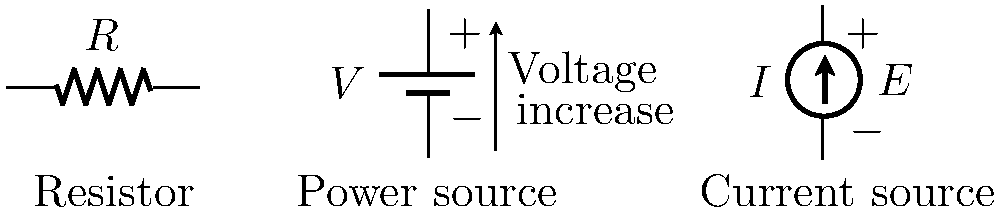
\includegraphics[width=4in]{3_elements}}
\caption{Elements in resistor networks. 
\label{fig_elements}}
\end{figure}

In the network, the resistances of all resistors will be given. The 
voltage across all voltage sources and the currents through all current 
sources will be given. 
There are two basic questions to answer about a resistor network with these
components. 
\begin{description}
\item[basic problem:] Find the currents through each resistor 
and each power source and also the voltage drops across each 
current source. This problem is a {\em linear system} of equations and 
so serves as an example of the mathematical techniques learnt in this 
chapter. 
\item[fundamental problem:] An important sub-problem is to find the 
currents through every power source and the voltage drops across 
each current source. These quantities can be written in terms of the given 
voltages and current sources directly (eliminating the terms involving 
resistor currents). 
Later, solving this problem will tell us how to 
write a differential equation for the currents through inductors and 
the voltages across capacitors. 
\end{description}

There are two fundamental laws governing the behaviour of circuits that 
can be used to set up equations that can be solved to answer the questions 
above. They are Kirchhoff's laws:
\begin{enumerate}
\item The sum of voltage drops around any closed loops in the network 
must be zero. 
\item The sum of currents entering a node must be zero. 
\end{enumerate}

\subsection{Two Simple Examples Made Complicated}

Consider the simple network with one current source and one resistor 
shown in Figure~\ref{fig_simple} (left). Clearly, the current 
through the resistor must be $I$ and the voltage drop across the 
resistor must be $IR$ using Ohms Law (use the signs in the diagram 
for the direction of the drop). 


\begin{example}
\label{Ex:simple1} 
Consider the same example, introducing two nodes into the network 
as shown in Figure~\ref{fig_simple} (right). We now have three unknowns, 
$V_1$, $V_2$ and $I_2$. Find a linear system for these unknowns 
and then solve the system.
{\rm We have made this simple example more complicated 
but we will learn something as we work through it. Note that by specifying 
voltages at nodes (which will determine voltage drops across components)
we will always satisfy Kirchhoff's first law. Let us write down every other 
law that applies to this diagram:
\begin{eqnarray*}
I - I_2 & = & 0 \mbox{,\ \ Kirchhoff's second law at node 2} \\
I_2 - I & = & 0 \mbox{,\ \ Kirchhoff's second law at node 1} \\
V_2 - V_1 & = & I_2 R \mbox{,\ \ Ohm's Law over the resistor} 
\end{eqnarray*}
If you didn't look too closely, you might be happy thinking these 
are three equations for the three unknowns $I_2$, $V_1$ and $V_2$. 
However, rewriting gives 
\begin{eqnarray*}
I_2 & = & I \\
I_2 & = & I \\
V_2 - V_1 - I_2 R & = & 0 
\end{eqnarray*}
In augmented matrix form we can write the system and do Gaussian 
Elimination:
\[
\left[
\begin{array}{ccc}
1 & 0 & 0 \\
1 & 0 & 0 \\
-R & -1 & 1 
\end{array}
\right|
\left.
\begin{array}{ccc}
I \\ I \\ 0 
\end{array}
\right]
\sim 
\left[
\begin{array}{ccc}
1 & 0 & 0 \\
0 & -1 & 1 \\
0 & 0 & 0
\end{array}
\right|
\left.
\begin{array}{ccc}
I \\ -RI \\ 0 
\end{array}
\right]
\]
In the augmented matrix above, the unknowns are ordered $I_2$, $V_1$ 
and then $V_2$. The solutions are $I_2 = I$ (expected), $V_2 = s$ 
and $V_1 = s-RI$ where $s$ is a parameter that can take any value. 
This seems much more complicated that the intuitive solution at the 
beginning of this section. However, the conclusions are the same: 
the current through the resistor is $I$ and the voltage drop across 
the resistor is 
\[
V_2 - V_1 = s-(s-RI) = RI.
\]
The arbitrary constant in the voltage occurs here 
because no {\em reference} voltage has been specified (no point in the 
circuit has been grounded). }
\end{example} 

\begin{figure}
\centerline{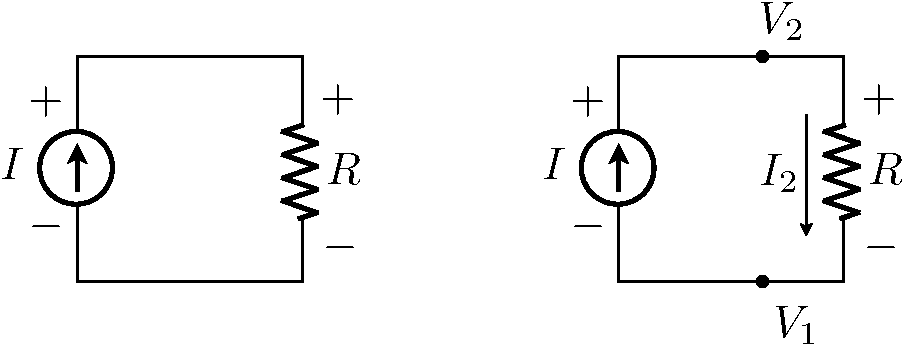
\includegraphics[width=4in]{3_simple}}
%\includegraphics[height=1.5in]{3_simple2}}
\caption{The simple resistor network considered in Example~\ref{Ex:simple1}. 
\label{fig_simple}}
\end{figure}

\begin{example} \label{Ex:simple2} Consider the circuit in Figure~\ref{fig_simple2}. 
Learning from the last example, we have set a reference voltage at the lower 
left corner of the circuit, and then voltage at the upper left corner is 
known. The current $I_1$ is the branch current from the $V_2$ node to the $V_1$ 
node. Form a linear system matching currents and voltages across resistors 
to Ohms Law, and matching branch currents at the two nodes. Solve the linear system.  
{\rm There are 5 unknowns $V_1$, $V_2$, $I_1$, $I_2$ and $I_3$ in the circuit 
as shown in the figure (the augmented matrices below will be written 
with the unknowns in this order). Ohm's law on the four resistors gives the following 
linear equations (in order of small to large resistance) 
\begin{eqnarray*}
12-V_1 & = & I_1 \\
V_1-V_2 & = & 2I_2 \\
V_1-V_2 & = & 3I_3 \\
V_2 & = & 4I_1 
\end{eqnarray*}
and matching the currents at the two nodes gives 
\begin{eqnarray*}
I_1 & = & I_2 + I_3 \\
I_2 + I_3 & = & I_1 
\end{eqnarray*}
This gives six equations in five unknowns! (maybe you already see why this happened 
to us). Writing the six equations above in an augmented matrix gives 
\[
\left[
\begin{array}{ccccc}
-1 & 0 & -1& 0 & 0  \\
1 & -1 & 0 & -2 & 0 \\
1 & -1 & 0 & 0 & -3 \\
0 & 1 & -4 & 0 & 0 \\
0 & 0 & 1 & -1 & -1 \\
0 & 0 & -1 & 1 & 1  
\end{array}
\right|
\left.
\begin{array}{c}
-12 \\ 0 \\ 0\\0\\0\\0
\end{array}
\right]
\sim 
\left[
\begin{array}{ccccc}
1 & 0 & 0 & 0 & 0 \\
0 & 1 & 0 & 0 & 0 \\
0 & 0 & 1 & 0 & 0 \\
0 & 0 & 0 & 1 & 0 \\
0 & 0 & 0 & 0 & 1 \\
0 & 0 & 0 & 0 & 0 
\end{array}
\right|
\left.
\begin{array}{c}
2184/217 \\ 1680/217 \\ 420/217 \\ 252/217 \\ 168/217 \\ 0  
\end{array}
\right]
\]
On the left above is the result of Gaussian elimination to reduced row echelon form. 
The solutions for $V_1$, $V_2$, $I_1$, $I_2$ and $I_3$ can be read off the last column
of the augmented matrix after reduction ($V_1=2184/217$ etc.). Notice that 
the ``extra" equation became the bottom row (all zeros) in the reduced form, which 
indicates that there was redundant information given in the linear system. 
If you go back to the expressions for conservation of current at the two nodes above, 
it is easy to see that these two equations carry the same information. 
}
\end{example}

\begin{figure}
\centerline{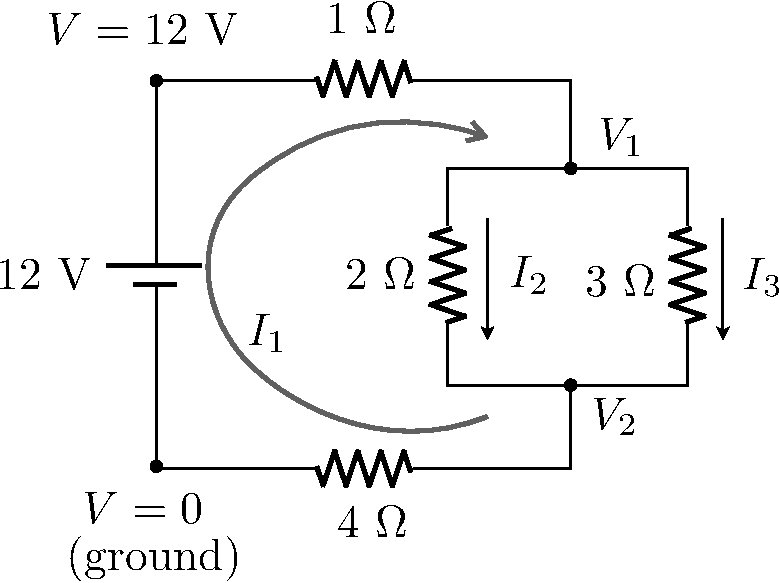
\includegraphics[height=2.5in]{3_resnet2010}}
\caption{The resistor network considered in Example~\ref{Ex:simple2}. 
\label{fig_simple2}}
\end{figure}

As the two previous examples show, one has to be a bit careful picking the unknowns 
and equations in a circuit to get a unique solution without introducing redundant 
equations. There are several ways to do this and when solving small circuits by hand 
the linear system can be made much simpler to solve if you pick the ``right" 
technique. In the next section we will describe the ``loop current" technique which 
always leads to a solvable linear system with no extra (redundant) equations.  

\subsection{Loop Currents}
\label{sec:loop}

We want to be able to see any resistor network and write down equations that 
will solve it uniquely, with no redundant equations like in the previous 
example and no non-uniqueness (like that coming from the 
lack of a reference potential). This can always be done using the 
following variables: loop currents, that is currents in every elementary 
loop of the network, and voltage drops across any current sources. This technique 
is described in more detail below.

Consider a circuit that can be drawn on a piece of paper with no
branches overlapping (a so-called planar network). The branches in the
circuit divide the diagram into smaller areas. The set of branches
around each of these small areas is called an elementary loop. By
assigning a \emph{loop current} to each elementary closed loop of the
circuit, the second of Kirchhoff's Circuit Laws is satisfied
automatically because in a closed loop the current entering any one
point is equal to the current travelling away from that point. Consider
Figure~\ref{labExf} (left). There are three elementary loops and loop
currents $i_1$, $i_2$ and $i_3$ associated with each of them. Loop
currents sum when they overlap in a branch. For example, the current
downwards through the 3 $\Omega$ resistor in Figure~\ref{labExf} is $i_2
- i_3$. Be careful of signs as you sum loop currents. In the example
above, $i_2$ is downwards through the 3 $\Omega$ resistor but $i_3$ is
upwards, hence it appears with a negative sign in our expression.

In a circuit, it is convenient to take loop currents and voltage drops
across current sources as the unknowns.  The first step in solving any
electric network is to identify the number of elementary loops in the
network. If there are $m$ independent loops present, then variables
$i_1,i_2,\ldots,i_m$ must be introduced to represent the loop
currents of each. If there are $n$ current sources, then the variables
$v_1, v_2, \ldots v_n$ must be introduced to represent the voltage
drop across each source. Together there are $n+m$ unknowns.

We can apply Kirchhoff's voltage law to each of the $m$ loops and
obtain $m$ linear equations for the unknowns. The current through each
current source must match the loop currents through it. This gives $n$
more linear equations for a total of $n+m$ linear equations for the
$n+m$ unknowns. 

\begin{example} 
\label{ex_resex2}
Solve the resistor network in Figure~\ref{fig_resex2}. Note that this is the same 
circuit as Example~\ref{Ex:simple2} but here the loop current method 
will be used. 
{\rm The unknowns are the loop currents 
$i_1$ and $i_2$ (there are no current sources). 
Remember that the loop currents add in shared components. For example, 
the current downwards in the 2$\Omega$ resistor is $i_1-i_2$. Using 
loop currents Kirchhoff's second law is always satisfied. The equations 
needed to solve for the loop currents are obtained by summing 
voltage drops around each elementary loop:
\begin{eqnarray*}
i_1 + 2(i_1-i_2) + 4i_1 - 12 & = & 0 
   \mbox{,\ \ voltage drops going around loop 1} \\
3i_2 + 2(i_2 - i_1) & = & 0 
   \mbox{,\ \ voltage drops going around loop 2.} 
\end{eqnarray*}
Collecting terms:
\begin{eqnarray*}
7 i_1 - 2i_2 & = & 12 \\
-2i_1 + 5i_2 & = & 0 
\end{eqnarray*}
which can be solved to give $i_2 = 24/31$ and $i_1 = 420/217$. With 
these values of $i_1$ and $i_2$ the current through each resistor 
and the power source can be determined, solving the problem. }
\end{example}

\begin{figure}
\centerline{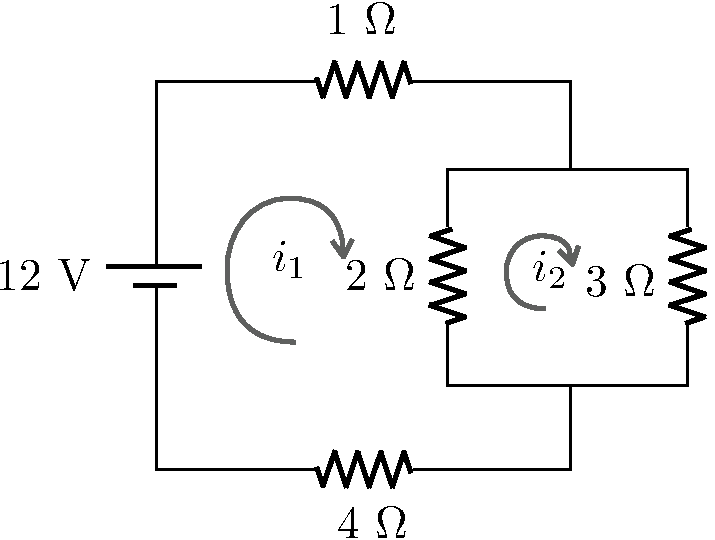
\includegraphics[height=1.5in]{3_resex2}}
\caption{The resistor network for Example~\ref{ex_resex2}
\label{fig_resex2}}
\end{figure}

There are easier ways to solve this {\em particular} small problem (the 
easiest is probably to use combinations of the series and parallel 
resistor laws). However, the loop current rule works for networks 
of arbitrarily large size and leads to systems of equations with a 
relatively small number of unknowns. On tests and exams, it is expected 
that students will be able to apply the idea of loop currents. 

\begin{example} 
\label{labEx} Solve the network shown in Figure~\ref{labExf}
{\rm There are three independent loop
currents which are labelled $i_1$, $i_2$ and $i_3$. There is a single 
current source  of $4A$ with voltage drop $v$ across it (minus to plus in the
direction of the current). There are also two $10V$ voltage sources.
Remember that the
current in an electrical branch shared by two loop currents is equal
to the (signed) sum of the two loops currents, \emph{i.e.} the current
moving to the left through the $5\Omega$ resistor of Figure \ref{labExf} is $i_1-i_
3$ and
thus the voltage drop is $5(i_1-i_3)$. Be careful also of the sign of
voltage drops. Moving around loop 1 in the circuit in Figure~\ref{labExf}
clockwise, when the current source is crossed, there a voltage
increase of $v$, so this would be a voltage {\em drop} of $-v$ in the
expression for Kirchhoff's second law for this loop written below.
We sum the voltage drops around loop 1 beginning at the current source
and moving clockwise (the same direction as $i_1$) to obtain
\[
-v + 2 i_1 + 5(i_1-i_3) + 2(i_1-i_2) = 0
\]
which can be simplified to 
\[
9i_1 -2 i_2 -5 i_3 -v = 0 
\]
The equations for the voltage drops around loops 2 and 3 are derived
similarly 
\[
\begin{array}{ccccccc}
-2i_1&+&5i_2&-& 3i_3 &=& -10 \\
-5i_1&-&3i_2&+& 8i_3 &=& \phantom{-}10
\end{array} 
\]
The final linear equation comes from matching the loop currents to the
current source:
\[
i_1 = 4
\]
The four linear equations above can be solved for the four unknowns $i_1, i_2, i_3, v$. 
The solution can be found using MATLAB (the details are in the computer lab \#4 
guide):
\[
\begin{array}{lcc}
i_1 &=& 4 {\rm A}\\
i_2 &\approx & 2.3871 {\rm A}\\
i_3 &\approx & 4.6452 {\rm A}\\
v & = & 8 {\rm V} 
\end{array}
\]
Now that the loop currents are determined, the branch currents can be
written down. For example the current over the $5\Omega$ resistor to
the right is 
$i_3-i_1 = 0.6452A$. The right hand panel of Figure \ref{labExf} displays
all six branch currents.}
\end{example}

\begin{figure}[htbp]
\centerline{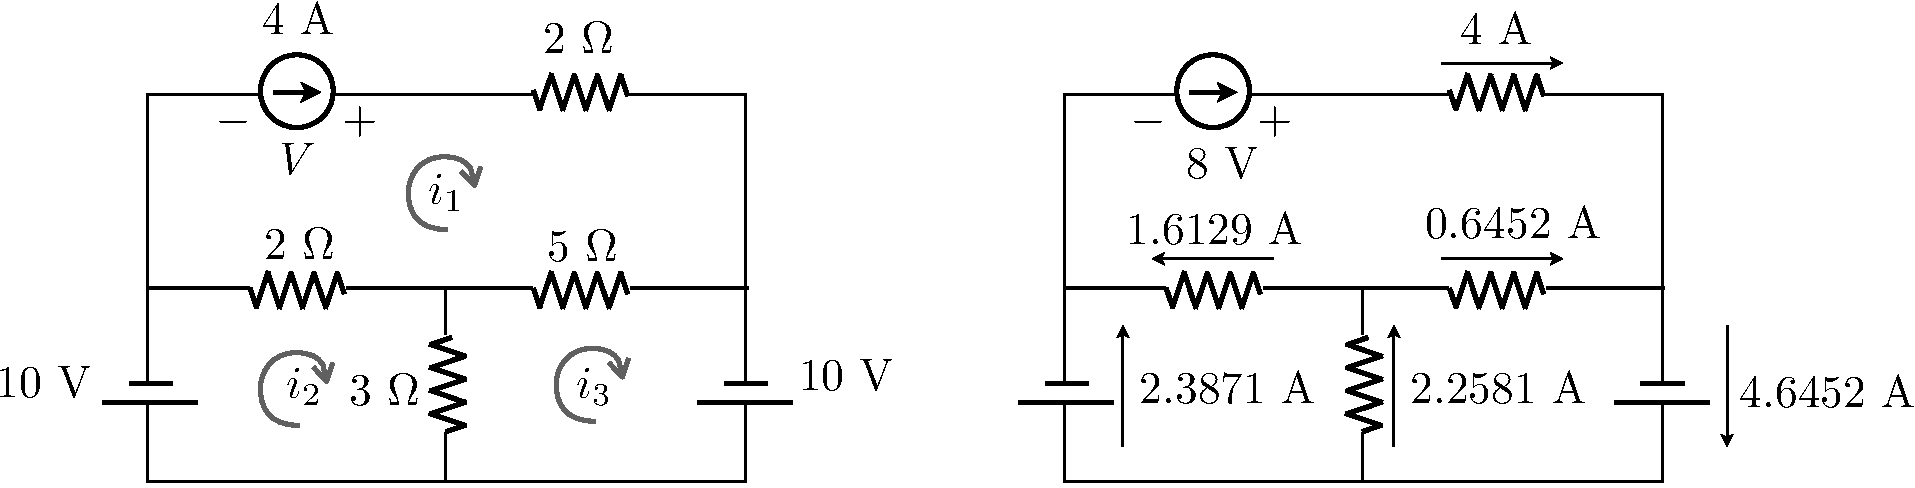
\includegraphics[width=5in]{3_lab4}}
\caption{\label{labExf} The left panel displays the schematic
circuit from Example~\ref{labEx} with two $10V$ voltage sources, 
four resistors and a current
source of $4A$. The loop currents $i_1$, $i_2$ $i_3$ represent the
current in each of the independent closed loops. The right panel is
the solution to the electric network on the left panel with branch
currents shown.}
\end{figure}

\begin{example} 
\label{ex_resex3}
Solve the resistor network in Figure~\ref{fig_resex3}. In this case, solve 
both the basic problem when $V=9$ and $I=1$, and then the fundamental problem
for arbitrary $V$ and $I$. 
{\rm The unknowns for the problem are $i_1$, $i_2$, $i_3$ and $E$. One 
equation in the system of unknowns comes from the fact that the loop 
current variables must match the current source:
\[
i_3= -I.
\]
Note that this equation is so simple we will no longer consider $i_3$ 
as a variable but replace $i_3$ by the known value $-I$ in the 
equations below. 
Voltage drops across the three loops give:
\begin{eqnarray*}
i_1 + 2(i_1-i_2) + 5i_1 - V & = & 0 \\
3(i_2 - i_3) + 2(i_2 - i_1) & = & 0 \\
5 i_3 + E + 3(i_3-i_2) & = & 0 
\end{eqnarray*}
Since $I$ and $V$ and $i_3$ (by the discussion above) are known 
quantities, we move them to the right hand side of the linear 
equations for $i_1$, $i_2$ and $E$ which are written below 
\begin{eqnarray}
\nonumber
8i_1 - 2i_2 & = & V \\
\label{eq_res4}
-2i_1 + 5i_2 & = & -3I \\
\nonumber 
-3i_2 + E & = & 8I.
\end{eqnarray}
With $V=9$ and $I=1$ this is solved using Gaussian Elimination to give 
the solution $E=7 \frac{1}{2}$, $i_2 = -1/6$ and $i_1= 13/12$. Note that the 
negative value for $i_2$ means that this loop current physically goes in the 
opposite direction to that in the Figure. For the 
fundamental problem, we consider (\ref{eq_res4}) for arbitrary values 
of $V$ and $I$. We write the system as an augmented matrix and do 
Gaussian Elimination with symbolic terms in the right hand sides:
\[
\left[
\begin{array}{ccc}
8 & -2 & 0 \\
-2 & 5 & 0 \\
0 & -3 & 1 
\end{array}
\right|
\left.
\begin{array}{c}
V \\ -3I \\ 8I 
\end{array}
\right] 
\sim 
\left[
\begin{array}{ccc}
1 & -1/4 & 0 \\
0 & 1 & 0 \\
0 & 0 & 1 
\end{array}
\right|
\left.
\begin{array}{c}
V/8 \\ -2/3I +V/18 \\ 6I + V/6
\end{array}
\right] 
\]
so $E=6I + V/6$ (the voltage across the current source in terms of the 
given voltage and currents of sources) and (after some algebra) 
$i_1 = \frac{10}{72} V - \frac{1}{6} I$ (the current through the
power source). An alternate approach to solving the fundamental 
problem is given in next section.}
\end{example} 

\begin{figure}
\centerline{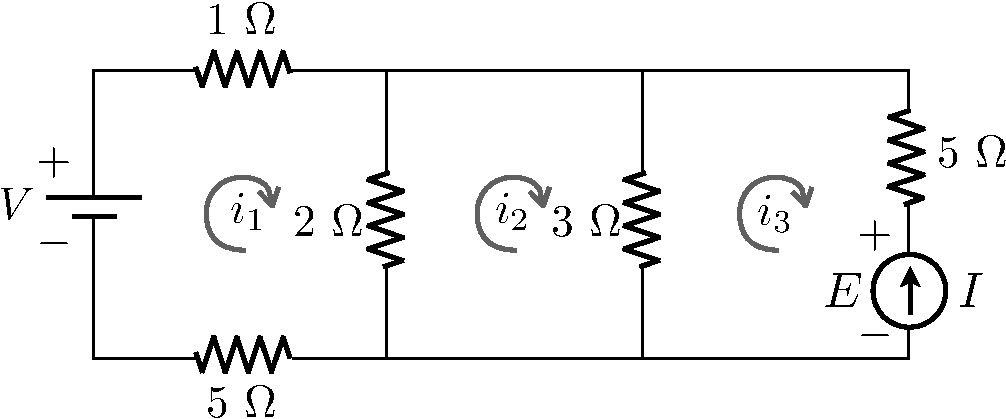
\includegraphics[width=4in]{3_resex3}}
\caption{The resistor network for Example~\ref{ex_resex3}
\label{fig_resex3}}
\end{figure}

\subsection{Alternate Presentation of Resistor Networks}
\label{sub_alternate}

Linear systems from resistor networks was presented in a previous 
version of the notes in a different way. That previous presentation 
is reproduced here beginning in the next paragraph. This alternate 
explanation may be helpful to some students. 

\begin{figure}
\centerline{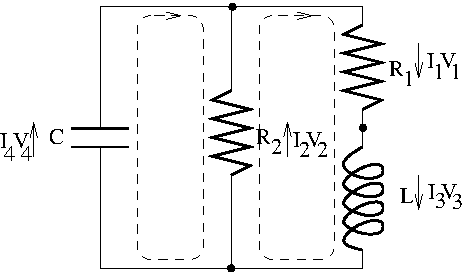
\includegraphics[height=1.5in]{3_circuit}}
\caption{A resistor network. 
\label{fig_circuit}}
\end{figure}

Consider the circuit shown in Figure~\ref{fig_circuit}. 
We won't be able to solve this circuit until we a studied differential equations
in the last part of this course. However we can make some progress
using what we know already.

There are three types of components: 
resistors, inductors (coils) and capacitors.
Associated with each component is the current $I$ flowing through that
component, and the voltage drop $V$ across that component. If there are $n$
different components in a circuit, then there are $2n$ variables (currents and
voltages) to determine. In the circuit above there are $8$.

Of course, these variables are not all independent. They satisfy two types of
linear relations: algebraic and differential. We won't touch the differential
relations for now, but we can consider the algebraic relations.

The first algebraic relation relates the current and voltage drop across a
resistor. If $R$ is the resistance and $I$ and $V$ are the current and voltage
drop respectively, then $V=IR$. In our example, this gives two equations
\begin{eqnarray*}
V_1&=&I_1R_1 \\
V_2&=&I_2R_2 \\
\end{eqnarray*}

The other two algebraic relations are Kirchhoff's laws. The first of these states
that the total voltage drop across any loop in the circuit is zero. For the two
loops in the example circuit, this gives the equations
\begin{eqnarray*}
V_4-V_2&=&0 \\
V_1+V_3+V_2&=& 0
\end{eqnarray*}
Notice we have to take the direction of the arrows into account. The second
Kirchhoff law states that current cannot accumulate at a node. At each node,
the current flowing in must equal the current flowing out. In the example
circuit there are three nodes, giving the equations.
\begin{eqnarray*}
I_4+I_2-I_1&=&0 \\
I_1-I_3&=&0 \\
I_3-I_2-I_4&=&0
\end{eqnarray*}

We now want to pick a few
of the variables, and solve for all the rest in terms of these. In a small
circuit like the example, this can be done ``by hand.''  For example, its pretty
obvious that $I_1=I_3$ and $V_2=V_4$ so one could eliminate two variables right off the
bat.
However, it is also useful
to have a systematic way of doing it, that will work for any circuit (but probably
will require a computer for anything but the simplest circuit).

As a rule of thumb, you can pick the voltages across the capacitor and the
currents across the inductors as basic variables and solve for the rest in
terms of these. In other words, we want $I_3$ and $V_4$ to be {\it parameters}
when we solve the system of equations. To accomplish this we will choose the
order of the variables with $I_3$ and $V_4$ at the end of the list. With this
in mind we choose the order $I_1,I_2,I_4,V_1,V_2,V_3,I_3,V_4$. Then the
equations become
\[
\matrix{
R_1I_1  &   &   &-V_1   &   &   &   &   &=0\cr
    &R_2I_2 &   &   &-V_2   &   &   &   &=0\cr
    &   &   &   &-V_2   &   &   &+V_4   &=0\cr
    &   &   &V_1    &+V_2   &+V_3   &   &   &=0\cr
-I_1    &+I_2   &+I_4   &   &   &   &   &   &=0\cr
I_1 &   &   &   &   &   &-I_3   &   &=0\cr
    &-I_2   &-I_4   &   &   &   &+I_3   &   &=0\cr
}
\]
The matrix for this system is (since it is a homogeneous system of equations,
we don't have to bother writing the augmented part)
\[
\left[\matrix{
R_1 &0  &0  &-1 &0  &0  &0  &0  \cr
0   &R_2    &0  &0  &-1 &0  &0  &0  \cr
0   &0  &0  &0  &-1     &0  &0  &1  \cr
0   &0  &0  &1  &1  &1  &0  &0  \cr
-1  &1  &1  &0  &0  &0  &0  &0  \cr
1   &0  &0  &0  &0  &0  &-1 &0  \cr
0   &-1 &-1 &0  &0  &0  &1  &0  \cr
}\right]
\]
Here is the reduced form of this matrix.
\[
\left[\matrix{
1   &0  &0  &0  &0  &0  &-1 &0  \cr
0   &1  &0  &0  &0  &0  &0  &-{{1}\over{R_2}}   \cr
0   &0  &1  &0  &0  &0  &-1 &{{1}\over{R_2}}    \cr
0   &0  &0  &1  &0  &0  &-R_1   &0  \cr
0   &0  &0  &0  &1  &0  &0  &-1 \cr
0   &0  &0  &0  &0  &1  &R_1    &1  \cr
0   &0  &0  &0  &0  &0  &0      &0      \cr
}\right]
\]
Thus
\begin{eqnarray*}
I_1&=&I_3 \\
I_2&=&{{1}\over{R_2}}V_4 \\
I_4&=&I_3-{{1}\over{R_2}}V_4 \\
V_1&=&R_1I_3 \\
V_2&=&V_4 \\
V_3&=&-R_1I_3-V_4 \\
\end{eqnarray*}
So we have succeeded in expressing all the variables in terms of 
$I_3$ and $V_4$. We
therefore need only determine these to solve the circuit completely.

\subsection{Problems}

\begin{problem}
\label{np3_1} 
Find the currents and voltages in each component of the 
circuit shown in Figure~\ref{fig_netprob} (left).
\end{problem}

\begin{problem}
\label{np3_2}
The resistances of the resistors shown in the circuit shown in 
Figure~\ref{fig_netprob} (right) are 
$R_1 = 4 \Omega$, $R_2 = 1 \Omega$, $R_3 = R_4 = 2 \Omega$. Find the 
current $I_2$ that flows through resistor $R_2$ if the voltage across 
the batteries are $E_1 = 5V$ and $E_2 = 3V$. In which direction 
does $I_2$ flow? Solve the problem as a system of linear equations 
for the loop currents $i_1$ and $i_2$ shown in the diagram. 
\end{problem}

\begin{figure}
\centerline{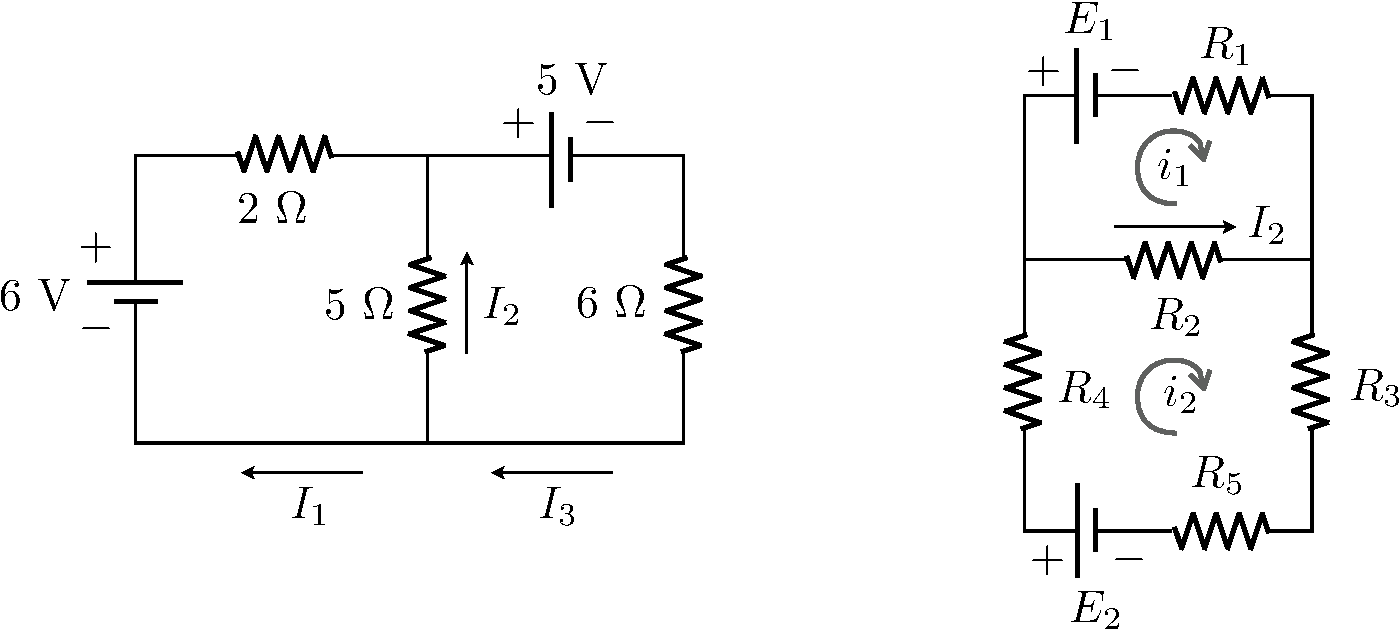
\includegraphics[width=5in]{3_netprob}}
%\hspace{5mm}
%\includegraphics[height=1.25in]{3_netprob2}}
\caption{Circuit diagrams for Problems~\ref{np3_1} (left) and 
\ref{np3_2} (right). 
\label{fig_netprob}}
\end{figure}

\begin{problem}
\label{2009_a5_3}
Consider the resistor network:

\begin{center}
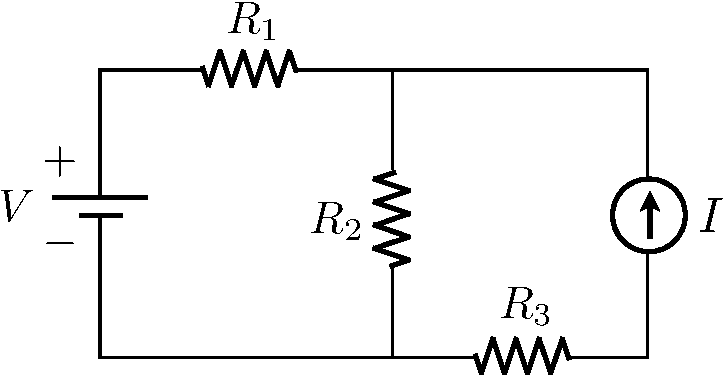
\includegraphics[height=1.25in]{3_fig5_3}
\end{center}
Given $R_1=3[\Omega]$, $R_2=1[\Omega]$, $R_3=4[\Omega]$, $V=26[V]$ and $I=2[A]$, answer the following questions:
\begin{enumerate}[a)]
\item What is the voltage drop through $R_3$?
\item What is the current flow through $R_2$?
\item What is the voltage drop through $R_1$?
\end{enumerate}
\end{problem}

\begin{problem}
\label{2009_a5_4}
Consider the following resistor network:

\begin{center}
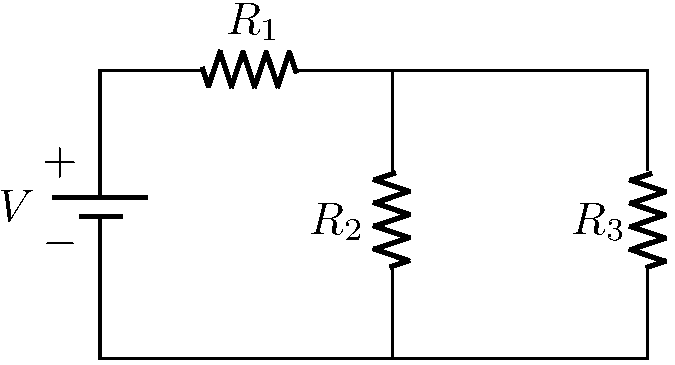
\includegraphics[height=1.25in]{3_fig5_1}
\end{center}
Suppose that $R_1=4[\Omega]$, $R_2=1[\Omega]$, $R_3=2[\Omega]$ and that the current flow through $R_3$ is $1.5[A]$. Solve the resistor network and answer the following questions:
\begin{enumerate}[a)]
\item What is the voltage drop across $R_3$?
\item What is the current flow through $R_2$?
\item What is the voltage drop through $V$?
\end{enumerate}
\end{problem}

\begin{problem}
\label{2009_a5_5}
Consider the following resistor network:

\begin{center}
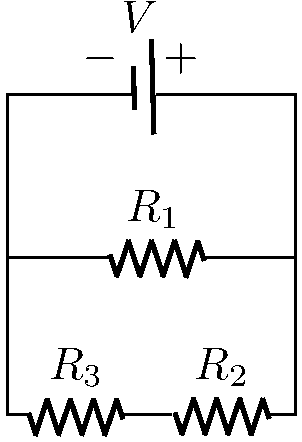
\includegraphics[height=1.25in]{3_fig5_2}
\end{center}
Suppose that $R_1=4[\Omega]$, $R_2=2[\Omega]$, $R_3=10[\Omega]$ and that $V=60[V]$. Solve the resistor network and answer the following questions:

\begin{enumerate}[a)]
\item What is the voltage drop through $R_2$?
\item What is the current flow through $R_1$?
\item What is the current flow through $R_3$?
\end{enumerate}
\end{problem}

\begin{problem}
\label{2009_a6_1}
Find the loop currents $i_1,i_2,i_3$ in the following network:

\centerline{\includegraphics[height=1.5in]{3_fig6_1}}


where $R_1=1[\Omega]$, $R_2=3[\Omega]$, $R_3=5[\Omega]$, $R_4=2[\Omega]$, $E_1=10[V]$ and $E_2=4[V]$.
\end{problem}

\begin{problem}
\label{2009_a6_2}
Consider the following network:

\centerline{\includegraphics[height=1.5in]{3_fig6_2}}

where $R_1=1[\Omega]$, $R_2=2[\Omega]$, $R_3= 1 [\Omega]$, $R_4=1 [\Omega]$,
$V=25[V]$ and $I=3[A]$.
\begin{enumerate}[a)]
\item Set up and solve the linear system for the
loop currents $i_1,i_2,i_3$ and the voltage $E$ across the current source.
\item What is the voltage drop across $R_2$?
\item What is the current flow through the voltage source $V$?
\end{enumerate} 
\end{problem}

%\begin{problem}
%\label{2009_a6_3}
%Consider the resistor network:
%
%\centerline{\includegraphics[height=1.5in]{3_fig6_3}}
%
%with $R_1=2[\Omega]$, $R_2=5[\Omega]$, $R_3=3[\Omega]$, $V=10[V]$, $I_1=3[A]$. Suppose that the voltage drop through $I_2$ is $E_2=5[V]$.
%\begin{enumerate}[a)]
%\item What is the current flow through $R_2$?
%\item What is the voltage drop through $I_1$?
%\item What is the current flow through $I_1$?
%\end{enumerate}
%\end{problem}

\begin{problem}
\label{op2_17}
If a circuit contains only resistors, then we can solve it completely 
using the ideas
of this section. 
Write down the linear equations satisfied by the currents in the
circuit shown in Figure~\ref{fig_circuit2}. 
In this diagram, the component on the far left is a voltage
source (battery). The voltage across the voltage source is always $E$.
\end{problem}

\begin{figure}
\centerline{\includegraphics[height=1.5in]{3_circuit2}}
\caption{The circuit from Problem~\ref{op2_17}.
\label{fig_circuit2}}
\end{figure}

\section{Additional Topics}

\subsection{The Check Column}
\label{s:check} 

Ordinary arithmetic errors are a big problem when you do row operations
by hand. There is a technique called ``the check column'' (that is modeled
after the ``parity bit'' in computer hardware design) which provides a
very effective way to catch mechanical errors. Here is an example which
illustrates the technique:

\begin{example} 
The augmented matrix for the system of equations
\[
\begin{array}{rrrrrrr}
  2x_1&+&x_2&+&3x_3&=\,&1 \\
  4x_1&+&5x_2&+&7x_3&=\,&7\cr
  2x_1&-&5x_2&+&5x_3&=\,&-7\cr
 \end{array} 
\]
is
\[
\left[ \begin{array}{ccc|c} 2&1&3 & 1 \\  4&5&7&7 \\  2&-5 &5 & -7 \end{array} \right]
\]
To implement a ``check column'' you tack onto the right hand side of the 
augmented matrix an additional column. Each entry in this check column is 
the sum of all the entries in the row of the augmented matrix that is to 
the left of the check column entry. For example, the top entry in the check
column is $2+1+3+1=7$.
\[
\left[ \begin{array}{ccc|c} 2&1&3 & 1 \\  4&5&7&7 \\  2&-5 &5 & -7 \end{array} \right]
\begin{array}{c} 7 \\ 23 \\ -5 \end{array} 
\]
To use the check column you just perform the same row
operations on the check column as you do on the augmented matrix. After
each row operation you check that each entry in the check column is
still the sum of all the entries in the corresponding row of the augmented
matrix.

We now want to eliminate the $x_1$'s from equations (2) and (3). That is,
we want to make the first entries in rows 2 and 3 of the augmented matrix
zero. We can achieve this by subtracting two times row (1) from row (2) and 
subtracting row (1) from row (3).
\[
\begin{array}{c} (1) \\ (2)-2(1) \\ (3)-(1) \end{array} 
\left[ \begin{array}{ccc|c} 2&1&3 & 1 \\  0&3&1&5 \\  0&-6 &2 & -8 \end{array} \right]
\begin{array}{c} 7 \\ 9 \\ -12 \end{array} 
\]
Observe that the check column entry $9$ is the sum $0+3+1+5$ 
of the entries in the second row of the augmented matrix. If this were
not the case, it would mean that we made a mechanical error. Similarly
the check column entry $-12$ is the sum $0-6+2-8$.

We have now succeeded in eliminating all of the $x_1$'s from equations
(2) and (3). For example, row 2 now stands for the equation
\[
3x_2+x_3=5
\]
We next use equation (2) to eliminate all $x_2$'s from equation
(3).
\[
\begin{array}{c} (1) \\ (2) \\ (3)+2(2) \end{array} 
\left[ \begin{array}{ccc|c} 2&1&3 & 1 \\  0&3&1&5 \\  0& 0&4 & 2 \end{array} \right]
\begin{array}{c} 7 \\ 9 \\ 6 \end{array} 
\]
We can now easily solve (3) for $x_3$, substitute the result back into (2) and
solve for $x_2$ and so on:
\begin{eqnarray*}
(3) &\rightarrow & 4x_3 =2  \rightarrow x_3 = \frac{1}{2} \\
(2) &\rightarrow & 3x_2 +\frac{1}{2} =5  \rightarrow x_2 = \frac{3}{2} \\
(1) &\rightarrow & 2x_1 + \frac{3}{2} + 3 \times \frac{1}{2} =1  \rightarrow x_1 = -1
\end{eqnarray*}
This last step is called ``backsolving''.
\end{example} 

Note that there is an easy way to make sure that we have not made any mechanical
errors in deriving this solution --- just substitute the purported solution
$(-1,3/2,1/2)$ back into the original system:
\[
\begin{array}{rrrrrrr}
  2(-1)&+& \frac{3}{2} &+&3 \times \frac{1}{2} &=\,&1 \\
  4(-1)&+&5\times \frac{3}{2}&+&7 \times \frac{1}{2}&=\,&7\cr
  2(-1)&-&5\times \frac{3}{2} &+&5 \times \frac{1}{2}&=\,&-7\cr
 \end{array} 
\]
and verify that each left hand side really is equal to its corresponding
right hand side. However, if this test fails, all we would know is that we had made an error somewhere in the elimination process. The check column technique can identify the place where the error was made. 

\subsection{Quadratic Functions}

Let begin by recalling how we would find the minimum of a quadratic function in
one variable, namely a parabola given by $f(x) = a x^2 + bx + c$ as
shown in Figure~\ref{fig_parabola}. We simply find
the value of $x$ for which the derivative is zero, that is, we solve $f'(x)=0$.
Notice that since $f$ is quadratic, this is a linear equation
\[
2ax+b=0
\]
which is easily solved for $x=-b/2a$ (provided $a\ne 0$). 
So the minimum value is $f(-b/2a) = -b^2/(4a) + c$.

\begin{figure}
\centerline{\includegraphics[height=1.5in]{3_parabola}}
\caption{The minimization of a quadratic function in one variable. 
\label{fig_parabola}}
\end{figure}

Of course, if $a$ is negative, then the parabola points downwards, and
we have found the maximum value, not the minimum value.

A quadratic function of two variables $x_1$ and $x_2$ is a function of the
form
\[
f(x_1,x_2)= ax_1^2 + 2bx_1x_2 + cx_2^2 + dx_1 + ex_2+f.
\]
(The $2$ in front of $b$ is just for convenience.) For what values of
$x_1$ and $x_2$ is $f(x_1,x_2)$ the smallest? Just like with the parabola in
one variable, there may be no such values. It could be that $f$ has a maximum
instead, or that $f$ has what is called a {\em saddle point}. However if $f$ does have
a minimum, the procedure described below is guaranteed to find it. (If $f$
has a maximum or saddle point, the procedure will find these points instead.)

The idea behind finding the minimum is simple. Suppose that $x_1$ and
$x_2$ are the values for which $f(x_1,x_2)$ is smallest. Then the function
$g(s) = f(x_1+s,x_2)$ must have a minimum at $s=0$. So $g'(0)=0$. But
\begin{eqnarray*}
g'(s) &=& {{d}\over{ds}}f(x_1+s,x_2) \\
&=&{{d}\over{ds}}a(x_1+s)^2 + 2b(x_1+s)x_2 + cx_2^2 +
d(x_1+s) + ex_2+f \\
&=& 2a(x_1+s) + 2bx_2 + d
\end{eqnarray*}
so that the condition is
\[
g'(0) = 2ax_1 + 2bx_2 + d = 0.
\]
Notice that this expression can be obtained by holding $x_2$ fixed and
differentiating with respect to $x_1$. It is called the partial derivative of
$f$ with respect to $x_1$ and is denoted ${{\PA f}\over{\PA x_1}}$.

The same argument can be applied to $h(s)=f(x_1,x_2+s)$ (or 
${{\PA f}\over{\PA x_2}}$.)
This yields
\[
h'(0) = {{\PA f(x_1,x_2)}\over{\PA x_2}} = 2bx_1 + 2cx_2 + e = 0.
\]

Therefore we conclude that the pair of values $x_1$ and $x_2$ at which
$f$ achieves its minimum satisfy the system of linear equations
\[
\matrix{
2ax_1 &+ 2bx_2 &= -d\cr
2bx_1 &+ 2cx_2 &= -e\cr
}
\]
This is a $2$ by $2$ system with augmented matrix
\[
\left[\matrix{
2a&2b\cr
2b&2c\cr
}\right.\left|\matrix{
-d\cr -e\cr
}\right]
\]

This is easily generalized to $n$ variables. 
In this case the quadratic function is given by
\[
f(x_1,x_2,\ldots,x_n)=\sum_{i=1}^n\sum_{j=1}^n a_{i,j}x_ix_j
+\sum_{i=1}^nb_ix_i+c
\]
To see this is the same, let us expand out the first term when $n=2$. Then
\begin{eqnarray*}
\sum_{i=1}^n\sum_{j=1}^n a_{i,j}x_ix_j
&=&a_{1,1}x_1x_1+a_{1,2}x_1x_2+a_{2,1}x_2x_1+a_{2,2}x_2x_2 \\
&=& a_{1,1}x_1^2+(a_{1,2}+a_{2,1})x_1x_2+a_{2,2}x_2^2 
\end{eqnarray*}
So this is just the same as before with $a_{1,1}=a$, $a_{1,2}+a_{2,1}=2b$ and
$a_{2,2}=c$. Notice that we might as well assume that $a_{i,j}=a_{j,i}$, since
replacing both $a_{i,j}$ and $a_{j,i}$ with $(a_{1,2}+a_{2,1})/2$ doesn't change
$f$.

If this function $f$ has a minimum we can find it by generalizing the procedure
above. In other words we try to find values of $x_1,\ldots,x_n$ for which
$\PA f/\PA x_1 = \PA f/\PA x_2=\cdots=\PA f/\PA x_n=0$. This leads to a system
of $n$ linear equations whose associated augmented matrix is
\[
\left[\matrix{
2a_{1,1}&2a_{1,2}&\ldots&2a_{1,n}\cr
2a_{2,1}&2a_{2,2}&\ldots&2a_{2,n}\cr
\vdots&\vdots&&\vdots\cr
2a_{n,1}&2a_{n,2}&\ldots&2a_{n,n}\cr
}\right.\left|\matrix{
-b_1\cr -b_2\cr \vdots\cr -b_n\cr
}\right]
\]

\subsection{Least squares fit}

As a first application let us  consider the problem of finding the ``best''
straight line going through a collection of data points $(x_1,y_1),
(x_2,y_2),\ldots,(x_n,y_n)$. (Careful! the  $x_i$'s are not the unknowns in this
problem, but rather the known fixed data points, together with the $y_i$'s.)
Consider Figure~\ref{fig_leastsquares}. 
Which straight line fits best? There is no one answer. One can measure how good the fit of
a straight line is in various ways. However the following way of measuring the
fit results in a problem that is easy to solve.

\begin{figure}
\centerline{\includegraphics[height=1.5in]{3_leastsquares}}
\caption{Fitting a line through data.
\label{fig_leastsquares}}
\end{figure}

Each line is given by an equation $y=ax+b$. So the variables in this problem are
$a$ and $b$. We want to find the values of $a$ and $b$ that give the best
fitting line. The vertical distance between the point $(x_i,y_i)$ and the line
is given by $|y_i-ax_i-b|$. We will take as a measure of the fit, the square of
this quantity, added up over all the data points. So
\begin{eqnarray*}
f(a,b) &= &\sum_i (y_i-ax_i-b)^2 \\
&=&\sum_i\left(y_i^2+x_i^2a^2+b^2 -2x_iy_ia-2y_ib+2x_iab\right) \\
&=&\left(\sum_i x_i^2\right)a^2 +2\left(\sum_i x_i\right)ab + nb^2
-2\left(\sum_i x_iy_i\right)a -2\left(\sum_i y_i\right)b
+\left(\sum_i y_i^2\right)
\end{eqnarray*}
Here we used that $(\sum_i 1)=n$, the number of points.
Therefore the linear equations we must solve for $a$ and $b$ are
\[
\left[\matrix{
2\left(\sum_i x_i^2\right)&2\left(\sum_i x_i\right)\cr
2\left(\sum_i x_i\right)&2n\cr
}\right.\left|\matrix{
2\left(\sum_i x_iy_i\right)\cr 2\left(\sum_i y_i\right)\cr
}\right]
\]
We could solve these equations numerically in each particular case, but since
its just a $2$ by $2$ system we can also write down the answer explicitly.
In fact, the solution to
\[
\left[\matrix{
A&B\cr
C&D\cr
}\right.\left|\matrix{
E\cr F\cr
}\right]
\]
is
\[
\left[\matrix{{{DE-BF}\over{AD-BC}}\cr
{{AF-CE}\over{AD-BC}}\cr}\right],
\]
provided $AD-BC\ne0$,
as you may check directly, or derive using a sequence of row transformations.
So in this case
\begin{eqnarray*}
a&=&{{n(\sum x_iy_i)-(\sum x_i)(\sum y_i)}\over{n(\sum x_i^2)-
   (\sum x_i)^2}} \\
b&=&{{(\sum x_i^2)(\sum y_i)-(\sum x_i)(\sum x_iy_i)}
   \over{n(\sum x_i^2)-(\sum x_i)^2}} \\
\end{eqnarray*}

\begin{example}
\label{ex_lsfit}
Suppose we want to find the best straight line through
the points $(1,1)$, $(2,2)$, $(2,3)$, $(3,3)$ and $(3,4)$. 
{\rm Calculate
\[
\matrix{
\sum 1 &= n&= 5\cr
\sum x_i &= 1+2+2+3+3 &= 11\cr
\sum y_i &= 1+2+3+3+4 &= 13\cr
\sum x_i^2&= 1+4+4+9+9 &= 27\cr
\sum y_i^2&= 1+4+9+9+16 &= 39\cr
\sum x_iy_i&=1+4+6+9+12 &= 32\cr
}
\]
so
\[
a = (5\cdot 32-11\cdot 13)/(5\cdot 27-11^2) = 17/14 = 1.214\ldots
\]
and
\[
b = (27\cdot 13-11\cdot 32)/(5\cdot 27-11^2) = -1/14 = -0.0714\ldots
\]
The result is shown in Figure~\ref{fig_lsqeg}.}
\end{example}

\begin{figure}
\centerline{\includegraphics[height=1.5in]{3_lsqeg}}
\caption{The solution in Example~\ref{ex_lsfit}.
\label{fig_lsqeg}}
\end{figure}

\subsection{Equilibrium configuration of hanging weights and springs}

Consider the problem of $n$ vertically hanging weight connected by springs.
What is the equilibrium configuration? We can solve this problem by calculating
the total potential energy of the system. The equilibrium configuration
minimizes the total potential energy.
A diagram of the setup is shown in Figure~\ref{fig_springs}. 
Our goal is to compute the numbers $x_1$,
$\ldots$, $x_n$. In the diagram $n=3$.

\begin{figure}
\centerline{\includegraphics[height=1.5in]{3_springs}}
\caption{Equilibrium configuration of springs.
\label{fig_springs}}
\end{figure}

There are two sources of potential energy. One is the potential energy stored in
the spring. This is equal to $k s^2/2$, where $k$ is the spring constant that
measures the stiffness of the spring, and $s$ is the amount that the spring has
been stretched from its natural length. In our problem, suppose that the
spring constant of the $i$th spring is $k_i$ and its natural
length is $l_i$. Then the potential energy stored in the $i$th spring
is $k_i(x_{i}-x_{i-1}-l_i)^2/2$. To make this formula work out correctly for the
first spring we set $x_0=0$.

The other source of potential energy is gravity. The gravitational potential
energy of the $i$th weight is $-m_igx_i$. The reason for the minus sign is that
we are measuring distances downward.

Thus the total potential energy in the system for $n$ weights is the function
\[
f(x_1,x_2,\ldots, x_n) = \sum_{i=1}^n {{k_i}\over{2}}(x_{i}-x_{i-1}-l_i)^2 - m_igx_i.
\]
When $n=3$ this becomes
\[
f(x_1,x_2,x_3) = {{k_1}\over{2}}(x_1-l_1)^2 + {{k_2}\over{2}}(x_2-x_1-l_2)^2
+{{k_3}\over{2}}(x_3-x_2-l_3)^2 -m_1gx_1-m_2gx_2-m_3gx_3
\]
This is a quadratic function, so we know how to find the minimum. The equations
are obtained by taking partial derivatives: To get the first equation we hold
$x_2$ and $x_3$ fixed and differentiate with respect to $x_1$ and so on. Thus
the equations are
\begin{eqnarray*}
k_1(x_1-l_1) - k_2(x_2-x_1-l_2) - m_1g &=&0 \\
k_2(x_2-x_1-l_2) - k_3(x_3-x_2-l_3) - m_2g &=&0 \\
k_3(x_3-x_2-l_3) -m_3g&=&0
\end{eqnarray*}
The augmented matrix for this system is
\[
\left[\matrix{
k_1+k_2&-k_2&0\cr
-k_2&k_2+k_3&-k_3\cr
0&-k_3&k_3\cr
}\right.\left|\matrix{
m_1g+k_1l_1-k_2l_2\cr m_2g+k_2l_2-k_3l_3\cr m_3g+k_3l_3\cr
}\right]
\]

\begin{example}
Suppose that the spring constants are $k_1=1$, $k_2=2$ and $k_3=1$. The
masses are all equal to $1$, $g=10$ and the natural length of the springs
is $1$ for all springs (in appropriate units). Find the equilibrium
configuration.
{\rm We must solve
\[
\left[\matrix{
3&-2&0\cr
-2&3&-1\cr
0&-1&1\cr
}\right.\left|\matrix{
9\cr 11\cr 11\cr
}\right]
\]
Gaussian elimination gives
\[
\left[\matrix{
3&-2&0\cr
0&-1&1\cr
0&0&2\cr
}\right.\left|\matrix{
9\cr 11\cr 106\cr
}\right]
\]
which can be solved to give $x_1=31$, $x_2=42$, $x_3=53$.}
\end{example}

\subsection{Problems}

\begin{problem}
\label{op2_13}
Find the ``best'' straight line going through the points
$(1,1)$, $(2,1)$, $(2,3)$, $(3,4)$, $(3,5)$ and $(4,4)$.
\end{problem}

\begin{problem}
\label{op2_14}
Consider the problem of finding the parabola $y=ax^2+bx+c$ that best fits the n
data points $(x_1,y_1)\ldots (x_n,y_n)$. Derive the system of three linear
equations which determine $a$, $b$ and $c$. (You need not solve solve them!)
\end{problem}

\begin{problem}
\label{op2_15}
Write down the augmented matrix for a system of $n$ weights and springs.
\end{problem}

\begin{problem}
\label{op2_16}
Write down the system of equations you would have to solve if there are
$5$ identical springs with $k_i=1$ and $l_i=1$ and five weights
with $m_1=1$, $m_2=2$, $m_3=3$, $m_4=4$, and $m_5=5$.
\end{problem}


\section{Solutions to Chapter Problems}

%%%%%%%%%%%%%%%%%%%%%%%%%%%%%%%%%%%%%%%%%%%%%%%%%%%%%%%%%%%%%%%%%%%%%%%%%%%%%%%%
\vspace{2mm}
\noindent {\bf Solution \ref{2009_a3_5}}
The augmented matrix is
$$
A = \left[\begin{array}{ccc|c}
  1 & -2 & 3 & 6\\
	4 & -5 & -6 & 7\\
	8 & 9 & 10 & 11
\end{array}\right]
$$


%%%%%%%%%%%%%%%%%%%%%%%%%%%%%%%%%%%%%%%%%%%%%%%%%%%%%%%%%%%%%%%%%%%%%%%%%%%%%%%%
\noindent {\bf Solution \ref{op2_1}}
Here is the sequence of systems of equations you would get:
\[
\matrix{
x_1&+&x_2&+&x_3&=&6\cr
x_1&-&x_2&+&x_3&=&0\cr
2x_1&+&x_2&-&8x_3&=&-11\cr
}
\]
%
\[
\matrix{
x_1&+&x_2&+&x_3&=&6\cr
&-&	2x_2&&	&=&	-6\cr
2x_1&+&x_2&-&8x_3&=&-11\cr
}
\]
%
\[
\matrix{
x_1&+&	x_2&+&	x_3&=&	6\cr
&-&	2x_2&&	&=&	-6\cr
&-&	x_2&-&	10x_3&=&	-23\cr
}
\]
%
\[
\matrix{
x_1&+&	x_2&+&	x_3&=&	6\cr
&&	x_2&&	&=&	3\cr
&-&	x_2&-&	10x_3&=&	-23\cr
}
\]
%
\[
\matrix{
x_1&+&	x_2&+&	x_3&=&	6\cr
&&	x_2&&	&=&	3\cr
&&	&-&	10x_3&=&	-20\cr
}
\]
So $x_3=2$, $x_2=3$ and $x_1=1$.

%%%%%%%%%%%%%%%%%%%%%%%%%%%%%%%%%%%%%%%%%%%%%%%%%%%%%%%%%%%%%%%%%%%%%%%%%%%%%%%%
\vspace{2mm}
\noindent {\bf Solution \ref{matlab_op2_1}}
\begin{verbatim}
A = [1, 1, 1, 6; 1, -1, 1, 0; 2, 1, -8, -11]
A(2,:) = A(2,:) - A(1,:)
A(3,:) = A(3,:) - 2*A(1,:)
A(2,:) = -A(2,:)/2
A(3,:) = A(3,:) + A(2,:)
A(3,:) = -A(3,:)/10
\end{verbatim}
We get the same solution as in the pen-and-paper version in problem \ref{op2_1}.

%%%%%%%%%%%%%%%%%%%%%%%%%%%%%%%%%%%%%%%%%%%%%%%%%%%%%%%%%%%%%%%%%%%%%%%%%%%%%%%%
\vspace{2mm}
\noindent {\bf Solution \ref{2009_a3_4}}
Perform the sequence of operations to finally end up with the system
\begin{eqnarray*}
  2x_3 &=& 4 \\
	3x_1 - 3x_2 + 3x_3 &=& 30 \\
	9x_1 \hspace{27pt} + 2x_3 &=& 26.
\end{eqnarray*}
%
Hence, $x_1 = 22/9$, $x_2 = -50/9$, and $x_3 = 2$.


%%%%%%%%%%%%%%%%%%%%%%%%%%%%%%%%%%%%%%%%%%%%%%%%%%%%%%%%%%%%%%%%%%%%%%%%%%%%%%%%
\vspace{2mm}
\noindent {\bf Solution \ref{2009_a3_3}}
We want to solve the system
\begin{eqnarray*}
  2x_1 + x_2 &=& 5 \\
	3x_1 + 5x_2 &=& -10. \\
\end{eqnarray*}
We shall use the method of substitution.

From the first equation, we solve for $x_2$:
$$x_2 = 5 - 2x_1$$
We then substitute it into the second equation:
$$3x_1 + 5(5 - 2x_1) = -10$$.
We now have a decoupled equation, and the solution is $x_1 = 5$, $x_2 = -5$.

%%%%%%%%%%%%%%%%%%%%%%%%%%%%%%%%%%%%%%%%%%%%%%%%%%%%%%%%%%%%%%%%%%%%%%%%%%%%%%%%
\vspace{2mm}
\noindent {\bf Solution \ref{op2_2}}
The first equation reads $x_1=3$. The second reads $x_1-x_2=3$, or $3-x_2=3$, or
$x_2=0$. The third reads $2x_1+x_2-8x_3=-4$, or $6+0-8x_3=-4$ or $x_3=5/4$. 

%%%%%%%%%%%%%%%%%%%%%%%%%%%%%%%%%%%%%%%%%%%%%%%%%%%%%%%%%%%%%%%%%%%%%%%%%%%%%%%%
\vspace{2mm}
\noindent {\bf Solution \ref{op2_3}}
The last equation gives $x_4=2$ and the second last one $x_3=2$. Then we have to
introduce a parameter $x_2-s$ and the we find that $x_1=-5-2s$ Thus
$\xx=\left[\matrix{-5\cr 0\cr 2\cr 2\cr}\right] + s \left[\matrix{-2\cr 1\cr
0\cr 0\cr}\right]$
In the second system, we have to introduce a parameter right off the bat. So
$x_4=s_1$ and $x_3=4-s_1$. Moving up one row, we have to introduce another
parameter $x_2=s_2$ and then $x_1=1-2s_2-(4-s_1)-2s_1=-3-s_1-2s_2$
so $\xx=\left[\matrix{-3\cr 0\cr 4\cr 0\cr}\right] + s_1 \left[\matrix{-1\cr 0\cr
-1\cr 1\cr}\right] + s_2 \left[\matrix{-2\cr 1\cr
0\cr 0\cr}\right]$
The third system is just the same. The extra rows of zeros have no effect.

%%%%%%%%%%%%%%%%%%%%%%%%%%%%%%%%%%%%%%%%%%%%%%%%%%%%%%%%%%%%%%%%%%%%%%%%%%%%%%%%
\vspace{2mm}
\noindent {\bf Solution \ref{2009_a4_3}}
Perform the following sequence of row operations:
\begin{enumerate}[i)]
\item $(2,:) = (2,:) - (1,:)$
\item $(3,:) = (3,:) - (1,:)$
\item $(3,:) = (3,:) + 2(2,:)$
\item $(4,:) = (4,:) - 3(2,:)$
\item $(4,:) = (4,:) + (3,:)$,
\end{enumerate}
in order to get the reduced row echelon form (RREF)
$$
\left[\begin{array}{cccc|c}
     1 & 2 & 2 & 2 & 1 \\
		 0 & 1 & -3 & 1 & -2\\
		 0 & 0 & -7 & 1 & 0\\
		 0 & 0 & 0 & 0 & 0
      \end{array}\right].
$$
Thus, we have that the rank of the augmented matrix, which is the same as the rank of the unaugmented matrix is $r=3$, while the number of unknowns is $n=4$. Therefore, the system has infinitely many solutions, that can be represented as the general solution
$$
\xx = \qq + s\aa,
$$
where $s$ is any real number, $\qq = (q_1,q_2,q_3,q_4)$ is any particular solution of the original system, and $\aa = (a_1, a_2, a_3, a_4)$ is any non-zero solution of the corresponding homogeneous system.

From the row echelon form we can see that $\qq$ has to satisfy $- 7q_3 + q_4 = 0$. Let $q_4 = 7$, then $q_3 = 1$. For the other two $q$ values we have
\begin{eqnarray*}
  q_2 &=& -2 + 3q_3 - q_4 = -6 \\
	q_1 &=& 1 - 2q_2 - 2q_3 - 2q_4 = -3.
\end{eqnarray*}
Hence, we have that $\qq = (-3, -6, 1, 7)$.

Now, to find $\aa$, the homogeneous row echelon form is
$$
\left[\begin{array}{cccc|c}
     1 & 2 & 2 & 2 & 0 \\
		 0 & 1 & -3 & 1 & 0\\
		 0 & 0 & -7 & 1 & 0\\
		 0 & 0 & 0 & 0 & 0
      \end{array}\right].
$$
Thus, $\aa$ has to satisfy $-7a_3 + a_4 = 0$. Take $a_4 = 7$, then $a_3 = 1$.

From the second row we have that $a_2 = 3a_3 - a_4 = -4$, and from the first row we get that $a_1 = -2a_2 - 2a_3 - 2a_4 = -8$. So $\aa = (-8, -4, 1, 7)$, and a general form of the solution is
$$
\xx = \left[\begin{array}{c} -3 \\ -6 \\ 1 \\ 7 \end{array}\right] +
s\left[\begin{array}{c} -8 \\ -4 \\ 1 \\ 7 \end{array}\right]
$$

%%%%%%%%%%%%%%%%%%%%%%%%%%%%%%%%%%%%%%%%%%%%%%%%%%%%%%%%%%%%%%%%%%%%%%%%%%%%%%%%
\vspace{2mm}
\noindent {\bf Solution \ref{2009_a4_1}}
Perform the following sequence of row operations
\begin{enumerate}[i)]
\item $(2,:) = (2,:) - 3(1,:)$
\item $(4,:) = (4,:) - 2(1,:)$
\item $(4,:) = (4,:) + 2(3,:)$
\item $(3,:) \leftrightarrow (2,:)$
\item $(4,:) \leftrightarrow (3,:)$
\item $(4,:) = (4,:) - \frac{3}{2}(3,:)$,
\end{enumerate}
to transform the augmented matrix into the reduced row echelon form
$$
\left[\begin{array}{cccc|c}
     1 & 2 & 2 & -7 & 20 \\
		 0 & 6 & 0 & -6 & -10\\
		 0 & 0 & -6 & 0  & -30\\
		 0 & 0 & 0 & 16 & -30
      \end{array}\right].
$$
We can now solve the system starting from the bottom:
\begin{eqnarray*}
x_4 &=& -\frac{30}{16} = -\frac{15}{8} \\
x_3 &=& \frac{-30}{-6} = 5 \\
x_2 &=& \frac{-10 + 6x_4}{6} = -\frac{85}{24} \\
x_1 &=& 20 - 2x_2 - 2x_3 + 7x_4 = \frac{95}{24}
\end{eqnarray*}

%%%%%%%%%%%%%%%%%%%%%%%%%%%%%%%%%%%%%%%%%%%%%%%%%%%%%%%%%%%%%%%%%%%%%%%%%%%%%%%%
\vspace{2mm}
\noindent {\bf Solution \ref{op2_4}}
The matrix 
\[
\left[
\begin{array}{ccc}
1&-2&3 \\
2&-3&2 \\
3&2&-4 
\end{array} \right| \left.
\begin{array}{c}
2 \\ 2 \\ 9
\end{array}
\right]
\]
reduces to
\[
\left[
\begin{array}{ccc}
1&-3&3 \\
0&1&4 \\
0&0&19
\end{array} \right| \left.
\begin{array}{c}
2 \\ -2 \\ 19
\end{array}
\right]
\]
which has as solution
$x_1=3$, $x_2=2$, $x_3=1$.
%%%%%%%%%%%%%%%%%%%%%%%%%%%%%%%%%%%%%%%%%%%%%%%%%%%%%%%%%%%%%%%%%%%%%%%%%%%%%%%%

\vspace{2mm}
\noindent {\bf Solution \ref{op2_5}}
The matrix 
\[
\left[
\begin{array}{ccc}
2&1&-1 \\
1&-2&-2 \\
-1&12&8
\end{array} \right| \left.
\begin{array}{c}
6 \\ 1 \\ 7
\end{array}
\right]
\]
reduces to
\[
\left[
\begin{array}{ccc}
2&1&-1 \\
0&-5/2&-3/2 \\
0&0&0
\end{array} \right| \left.
\begin{array}{c}
6 \\ -2 \\ 0
\end{array}
\right]
\]
which has as solution
$x_1=13/5+4s/5$, $x_2=4/5-3s/5$, $x_3=s$.
%%%%%%%%%%%%%%%%%%%%%%%%%%%%%%%%%%%%%%%%%%%%%%%%%%%%%%%%%%%%%%%%%%%%%%%%%%%%%%%%

\vspace{2mm}
\noindent {\bf Solution \ref{op2_6}}
The matrix 
\[
\left[
\begin{array}{ccc}
1&2&4 \\
1&1&3 \\
2&5&9
\end{array} \right| \left.
\begin{array}{c}
1 \\ 2 \\ 1
\end{array}
\right]
\]
reduces to
\[
\left[
\begin{array}{ccc}
1&2&4 \\
0&-1&-1 \\
0&0&0
\end{array} \right| \left.
\begin{array}{c}
1 \\ 1 \\ 0
\end{array}
\right]
\]
Thus , setting $x_3=s$, we obtain $x_2 = -1-s$ and $x_1=3-2s$.

%%%%%%%%%%%%%%%%%%%%%%%%%%%%%%%%%%%%%%%%%%%%%%%%%%%%%%%%%%%%%%%%%%%%%%%%%%%%%%%%
\vspace{2mm}
\noindent {\bf Solution \ref{op2_7}}
The matrix 
\[
\left[
\begin{array}{ccc}
1&2&4 \\
1&1&3 \\
2&5&9
\end{array} \right| \left.
\begin{array}{c}
1 \\ 2 \\ 3
\end{array}
\right]
\]
reduces to
\[
\left[
\begin{array}{ccc}
1&2&4 \\
0&-1&-1 \\
0&0&0
\end{array} \right| \left.
\begin{array}{c}
1 \\ 1 \\ 2
\end{array}
\right]
\]
which has no solutions.
\bigskip

%%%%%%%%%%%%%%%%%%%%%%%%%%%%%%%%%%%%%%%%%%%%%%%%%%%%%%%%%%%%%%%%%%%%%%%%%%%%%%%%
\vspace{2mm}
\noindent {\bf Solution \ref{op2_8}}
The matrix 
\[
\left[
\begin{array}{cccc}
3&1&-1&2 \\
2&-2&5&-7 \\
-4&-4&7&-11
\end{array} \right| \left.
\begin{array}{c}
7 \\ 1 \\-13 
\end{array}
\right]
\]
reduces to
\[
\left[
\begin{array}{cccc}
3&1&-1&2 \\
0&-8/3&17/3&-25/3 \\
0&0&0&0
\end{array} \right| \left.
\begin{array}{c}
7 \\ -11/3 \\ 0
\end{array}
\right]
\]
which has as solution
$x_1=15/8-3s_1/8+3s_2/8$, $x_2=11/8+17s_1/8-25s_2/8$, $x_3=s_1$, $x_4=s_2$.

%%%%%%%%%%%%%%%%%%%%%%%%%%%%%%%%%%%%%%%%%%%%%%%%%%%%%%%%%%%%%%%%%%%%%%%%%%%%%%%%
\vspace{2mm}
\noindent {\bf Solution \ref{op2_9}}
Probably the easiest way to do this problem is to think geometrically. This
system of equations describes the intersection of two lines. The lines will
intersect in a single point if they are not parallel. This will happen exactly
when the two vectors $[a,b]$ and $[c,d]$ are not parallel. Recall that this can
be tested using the determinant. So the equations have a unique solution exactly
when $\det\left[\matrix{a&b\cr c&d\cr}\right]=ad-bc\ne0$.

%%%%%%%%%%%%%%%%%%%%%%%%%%%%%%%%%%%%%%%%%%%%%%%%%%%%%%%%%%%%%%%%%%%%%%%%%%%%%%%%
\vspace{2mm}
\noindent {\bf Solution \ref{2009_a4_2}}
Perform the following sequence of row operations:
\begin{enumerate}[i)]
\item $(2,:) = (2,:) - 4(1,:)$
\item $(3,:) = (3,:) + 4(1,:)$
\item $(3,:) = (3,:) + \frac{5}{3}(3,:)$
\end{enumerate}
to get the reduced row echelon matrix
$$
\left[\begin{array}{ccc|c}
     1 & 2 & 0 & 7 \\
		 0 & 0 & 6 & -18\\
		 0 & 0 & 0  & 139\\
      \end{array}\right].
$$
The last equation says $0=139$, which cannot happen, therefore this linear system has \textbf{zero} solutions.

%%%%%%%%%%%%%%%%%%%%%%%%%%%%%%%%%%%%%%%%%%%%%%%%%%%%%%%%%%%%%%%%%%%%%%%%%%%%%%%%
\vspace{2mm}
\noindent {\bf Solution \ref{matlab_2009_a4_2}}
The script is the following:
\begin{verbatim}
for a = 1:10
A = [1 2 4 7; 4 1 3 2; 0 5 9 a];
rref(A)
end
\end{verbatim}
If the value of $a$ changes linearly, then the solution to $x_1$ (or for that matter, of $x_2$ and $x_3$ too) changes linearly with $a$.

%%%%%%%%%%%%%%%%%%%%%%%%%%%%%%%%%%%%%%%%%%%%%%%%%%%%%%%%%%%%%%%%%%%%%%%%%%%%%%%%
\vspace{2mm}
\noindent {\bf Solution \ref{2009_a4_4}}
Perform the following sequence of row operations:
\begin{enumerate}[i)]
\item $(2,:) = (2,:) + (1,:)$
\item $(3,:) = (3,:) - (2,:)$
\end{enumerate}
to get the reduced row echelon matrix
$$
\left[\begin{array}{cccc|c}
     1 & 0 & 1 & 0 & 10 \\
		 0 & 1 & 2 & 1 & 14\\
		 0 & 0 & 0 & 0 & 0\\
      \end{array}\right].
$$
Thus the row echelon form for the corresponding homogeneous system is
$$
\left[\begin{array}{cccc|c}
     1 & 0 & 1 & 0 & 0 \\
		 0 & 1 & 2 & 1 & 0\\
		 0 & 0 & 0 & 0 & 0\\
      \end{array}\right].
$$
Let $\qq$ be any solution to the original system. For example, check that $\qq = (9,11,1,1)$ solves the system.

Now, let $\aa_1$ and $\aa_2$ be any two linearly independent vectors which solve the corresponding homogeneous system. For example, check that $\aa_1 = (1,1,-1,1)$, and $\aa_2 = (1,-1,-1,3)$ are two linearly independent vectors, which solve the homogeneous system.

Thus, one representation for the solutions of the system is
$$
\xx = \left[\begin{array}{c} 9 \\ 11 \\ 1 \\ 1 \end{array}\right] +
s_1\left[\begin{array}{c} 1 \\ 1 \\ -1 \\ 1 \end{array}\right] + s_2\left[\begin{array}{c} 1 \\ -1 \\ -1 \\ 3 \end{array}\right].
$$

%%%%%%%%%%%%%%%%%%%%%%%%%%%%%%%%%%%%%%%%%%%%%%%%%%%%%%%%%%%%%%%%%%%%%%%%%%%%%%%%
\vspace{2mm}
\noindent {\bf Solution \ref{op2_11}}
The general solution is $[4,0,3,0]+s_1[-1,1,0,0]+s_2[0,0,-2,1]$.

%%%%%%%%%%%%%%%%%%%%%%%%%%%%%%%%%%%%%%%%%%%%%%%%%%%%%%%%%%%%%%%%%%%%%%%%%%%%%%%%
\vspace{2mm}
\noindent {\bf Solution \ref{2009_a4_5}}
Perform the following sequence of row operations:
\begin{enumerate}[i)]
\item $(2,:) = (2,:) - (1,:)$
\item $(3,:) = (3,:) - \frac{1}{2}(2,:)$
\item $(2,:) = \frac{1}{12}(2,:)$
\item $(1,:) = (1,:) + 3(2,:)$
\end{enumerate}
to get the reduced row echelon matrix
$$
\left[\begin{array}{ccc|c}
     1 & 0 & \frac{1}{2} & 7 \\
		 0 & 1 & -\frac{7}{6} & 1/3 \\
		 0 & 0 & 0 & 0 \\
      \end{array}\right].
$$
Here the rank of the augmented matrix ($r_a=2$) is equal to rank of the unaugmented matrix ($r_u = 2$), therefore the linear system has solutions. Since $r_a = 2 < 3$ where 3 is the number of unknowns, there will be an infinite number of solutions with $x_3$ a free variable. 

%%%%%%%%%%%%%%%%%%%%%%%%%%%%%%%%%%%%%%%%%%%%%%%%%%%%%%%%%%%%%%%%%%%%%%%%%%%%%%%%
\vspace{2mm}
\noindent {\bf Solution \ref{op2_12}}
To decide whether the vectors are linearly independent we must decide
whether the homogeneous system of equations represented by the matrix
$\left[\matrix{1&1&1\cr 2&1&0\cr 0&-1&1\cr 2&1&0\cr}\right]$
has a non zero solution. Row reduction yields 
$\left[\matrix{1&1&1\cr 0&-1&-2\cr 0&0&3\cr 0&0&0\cr}\right]$.
This shows that the zero solution is unique and therefore the vectors
are independent. It can't happen that three vectors span a four dimensional
space. To test whether $\yy_1$ is a linear combination of the $\xx_i$'s
we try to solve the equation with augmented matrix
$\left[\matrix{1&1&1\cr 2&1&0\cr 0&-1&1\cr 2&1&0\cr}\right.\left|\matrix{2\cr 4\cr -3\cr 4\cr}\right]$.
Row reduction gives 
$\left[\matrix{1&1&1\cr 0&-1&-2\cr 0&0&3\cr 0&0&0\cr}\right.\left|\matrix{2\cr 0\cr -3\cr 0\cr}\right]$.
This system does have a solution, therefore the vector $\yy_1$ is a linear combination
of the $\xx_i$'s.

%%%%%%%%%%%%%%%%%%%%%%%%%%%%%%%%%%%%%%%%%%%%%%%%%%%%%%%%%%%%%%%%%%%%%%%%%%%%%%%%
\vspace{2mm}
\noindent {\bf Solution \ref{2009_a5_1}}
Three vectors in the plane cannot be linearly independent.

There are two ways to see that $y$ is a linear combination of $a_1$ and $a_2$:
\begin{itemize}
  \item $a_1$ and $a_2$ are linearly independent because
	$$
	\det\left[\begin{array}{cc}
	            1&2 \\ 3&1
	          \end{array}\right] = -5
	$$
	Therefore $\{a_1,a_2\}$ form a basis of $\mathbb{R}^2$, and every vector is a linear combination of $a_1$ and $a_2$.
	\item Solve the system
	$$
	x_1a_1+x_2a_2 = y
	$$
	i.e.
	$$
x_1\left[\begin{array}{c}1\\2\end{array}\right] + x_2\left[\begin{array}{c}3\\1\end{array}\right] = \left[\begin{array}{c}-15\\5\end{array}\right].
	$$
	This system yields the augmented matrix
\begin{eqnarray*}
&&\left[\begin{array}{cc|c}1&3&-15\\2&1&5\end{array}\right]\rarr (2,:)=(2,:)-2(1,:)\rarr \left[\begin{array}{cc|c}1&3&-15\\0&-5&35\end{array}\right]\\
&&\rarr (2,:)=-\frac{1}{5}(2,:)\rarr \left[\begin{array}{cc|c}1&3&-15\\0&1&-7\end{array}\right],
\end{eqnarray*}
which gives $x_2=7$, and $x_1 = 6$.
	
\end{itemize}


%%%%%%%%%%%%%%%%%%%%%%%%%%%%%%%%%%%%%%%%%%%%%%%%%%%%%%%%%%%%%%%%%%%%%%%%%%%%%%%%
\vspace{2mm}
\noindent {\bf Solution \ref{2009_a5_2}}
The vectors $a_1$, $a_2$, and $a_3$ are linearly independent if the only solution to the system
$$
x_1a_1 + x_2a_2 + x_3a_3 = 0
$$
is $x_1=x_2=x_3=0$
So,
\begin{eqnarray*}
&&\left[\begin{array}{ccc|c}1&0&10&0\\1&0&0&0\\0&4&-5&0\\0&-3&0&0\end{array}\right]\rarr \begin{array}{c}(2,:)=(2,:)-(1,:)\\(4,:)=-\frac{1}{3}(4,:)\end{array}\rarr
\left[\begin{array}{ccc|c}1&0&10&0\\0&0&-10&0\\0&4&-5&0\\0&1&0&0\end{array}\right]\\&&\rarr
\begin{array}{c}(2,:)=-\frac{1}{10}(2,:)\\(3,:)\lrarr(4,:)\end{array}\rarr
\left[\begin{array}{ccc|c}1&0&10&0\\0&0&1&0\\0&1&0&0\\0&4&-5&0\end{array}\right]\rarr
\begin{array}{c}(2,:)\lrarr(3,:)\\(4,:)=(4,:)-4(3,:)+5(2,:)\end{array}\\&&\rarr
\left[\begin{array}{ccc|c}1&0&10&0\\0&1&0&0\\0&0&1&0\\0&0&0&0\end{array}\right]
\end{eqnarray*}
The system has a unique solution $x_1=x_2=x_3=0$, hence the three vectors are linearly independent.

To find if $y$ can be written as a linear combination of the three vectors, we look for a solution of the system
\begin{eqnarray*}
&&\left[\begin{array}{ccc|c}1&0&10&11 \\ 1&0&0&1 \\ 0&4&-5&-1 \\ 0&-3&0&10\end{array}\right]\rarr \begin{array}{c}(2,:)=(2,:)-(1,:)\\(3,:)=(3,:)+(4,:)\end{array}\rarr
\left[\begin{array}{ccc|c}1&0&10&11 \\ 0&0&-10&-10 \\ 0&1&-5&9 \\ 0&-3&0&10\end{array}\right]\rarr\\
&&\begin{array}{c}(2,:)=-\frac{1}{10}(2,:)\\(4,:)=(4,:)+3(3,:)\end{array}\rarr
\left[\begin{array}{ccc|c}1&0&10&11 \\ 0&0&1&1 \\ 0&1&-5&9 \\ 0&0&-15&37\end{array}\right]
\end{eqnarray*}
The second row of the reduced row echelon matrix implies that $x_3=1$, while the third row yields that $x_3 = -\frac{37}{15}$. This contradiction means that the system has no solution, and $y$ is therefore not a linear combination of $a_1$, $a_2$, and $a_3$.

%%%%%%%%%%%%%%%%%%%%%%%%%%%%%%%%%%%%%%%%%%%%%%%%%%%%%%%%%%%%%%%%%%%%%%%%%%%%%%%%
\vspace{2mm}
\noindent {\bf Solution \ref{matlab_2009_a5_2}}
\begin{verbatim}
plot3([1,0],[2,0],[3,0])
hold on
plot3([-1,0],[2,0],[1,0])
plot3([4,0],[1,0],[-1,0])
\end{verbatim}
In the figure window, if you go to Tools $\rightarrow$ Rotate 3D, you will see right away that the three vectors do not share the same plane, therefore they must be linearly independent.

%%%%%%%%%%%%%%%%%%%%%%%%%%%%%%%%%%%%%%%%%%%%%%%%%%%%%%%%%%%%%%%%%%%%%%%%%%%%%%%%
\vspace{2mm}
\noindent {\bf Solution \ref{np3_1}}
We apply Kirchhoff's junction rule 
\[
I_1 + I_2 - I_3 = 0 
\]
and Kirchhoff's loop rules, moving around first the left loop and then
the right loop in a clockwise direction:
\begin{eqnarray*}
-2I_1 + 5I_2 + 6 & = & 0 \\
-5 - 6I_3 - 5I_2 & = & 0 
\end{eqnarray*}
Writing these three equations in an augmented matrix with the unknowns 
ordered $I_1$, $I_2$ and $I_3$ gives 
\[
\left[ \begin{array}{ccc}
1 & 1 & -1 \\
-2 & 5 & 0 \\
0 & -5 & -6 
\end{array}
\right| 
\left.
\begin{array}{c}
0 \\ -6 \\ 5
\end{array}
\right]
\]
which is solved to give $I_1 = 41/52$, $I_2 = -23/26$ and $I_3 = -5/52$ 
with units of Amperes. The voltage drops are $I_1 R_1 = 41/26$, 
$I_2 R_2 = 115/26$ and $I_3 R_3 = 15/26$ across the three resistors, 
with drops in the direction of positive currents. Note that this problem 
is more easily solved using two loop currents (try it and make sure you 
get the same solution). 

%%%%%%%%%%%%%%%%%%%%%%%%%%%%%%%%%%%%%%%%%%%%%%%%%%%%%%%%%%%%%%%%%%%%%%%%%%%%%%%%
\vspace{2mm}
\noindent {\bf Solution \ref{np3_2}}
We write voltage drops around the two loops in the direction of the 
loop currents:
\begin{eqnarray*}
4i_1 + (i_1-i_2) + 5 & = & 0 \mbox{\ \ or \ \ } 5i_1 - i_2 = -5 \\
(i_2-i_1) + 6i_2 -3  & = & 0 \mbox{\ \ or \ \ } -i_1 - i_2 = -5 
\end{eqnarray*}
which is solved to give $i_2 = 5/17$ and $i_1 = -16/17$. Thus, 
$I_2 = i_2-i_1 = 21/17$. Since it is positive, this current flows 
to the right.

%%%%%%%%%%%%%%%%%%%%%%%%%%%%%%%%%%%%%%%%%%%%%%%%%%%%%%%%%%%%%%%%%%%%%%%%%%%%%%%%
\vspace{2mm}
\noindent {\bf Solution \ref{2009_a5_3}}
\begin{figure}
\centerline{\includegraphics[height=1.25in]{3_fig5_3}}
\caption{Problem \ref{2009_a5_3}.
\label{fig_a5_3}}
\end{figure}
We use loop currents to solve the network depicted in figure \ref{2009_a5_3}.

Kirchhoff's second law gives that $i_2=-I$, and the first law applied to the closed loop on the left gives
$$
R_1i_1+R_2(i_1-i_2)=V.
$$
As $R_1 = 3[\Omega]$, $R_2=1[\Omega]$, $R_3 = 4[\Omega]$, $V=26[V]$, and $I=2[A]$, we get
\begin{eqnarray}
  &&i_2 = -2[A] \\
	&&3i_1+i_1+2=26
\end{eqnarray}
Hence $i_1 = 6[A]$, and from the sign we get that $i_2$ flows in the opposite direction as initially supposed.
\begin{enumerate}[a)]
\item Voltage drop $=R_3i_2=-8[V]$. The - sign indicates that the potential is higher at the left of $R_3$ than on the right.
\item The flow through $R_2$ is $i_1-i_2=8[A]$.
\item Voltage drop $=R_1i_1=18[V]$.
\end{enumerate}



%%%%%%%%%%%%%%%%%%%%%%%%%%%%%%%%%%%%%%%%%%%%%%%%%%%%%%%%%%%%%%%%%%%%%%%%%%%%%%%%
\vspace{2mm}
\noindent {\bf Solution \ref{2009_a5_4}}
Again, we use loop currents to solve the problem depicted in figure \ref{2009_a5_4}.
\begin{figure}
\centerline{\includegraphics[height=1.25in]{3_fig5_4}}
\caption{Problem \ref{2009_a5_4}.
\label{fig_a5_4}}
\end{figure}

\begin{eqnarray*}
  &&R_1i_1 + R_2(i_1-i_2) = V \\
	&&R_3i_2 + R_2(i_2-i_1) = 0,
\end{eqnarray*}
% 
with $R_1 = 4[\Omega]$, $R_2 = 1[\Omega]$, $R_3 = 2[\Omega]$.

The flow through $R_3$ is $i_2$, which is $1.5[A]$. The system becomes
$$
\left\{\begin{array}{c}4i_1+(i_1-1.5)=V \\ 3+(1.5-i_1)=0 \end{array}\right.
$$
$$
\left\{\begin{array}{c}5i_1-V=\frac{3}{2} \\ i_1=\frac{9}{2} \end{array}\right.
$$
Therefore $V=21[V]$, and $i_1=4.5[A]$
\begin{enumerate}[a)]
\item Voltage drop $=R_3i_2=3[V]$.
\item Current flow $=i_1-i_2=3[A]$.
\item Voltage drop $=V=21[V]$
\end{enumerate}

%%%%%%%%%%%%%%%%%%%%%%%%%%%%%%%%%%%%%%%%%%%%%%%%%%%%%%%%%%%%%%%%%%%%%%%%%%%%%%%%
\vspace{2mm}
\noindent {\bf Solution \ref{2009_a5_5}}
\begin{figure}
\centerline{\includegraphics[height=2.25in]{3_fig5_5}}
\caption{Problem \ref{2009_a5_5}.
\label{fig_a5_5}}
\end{figure}
As before:
$$
\left\{\begin{array}{c}R_1(i_1-i_2)=V \\ R_2i_2+R_3i_2+R_1(i_2-i_1)=0 \end{array}\right.,
$$
with $R_1 = 4[\Omega]$, $R_2 = 2[\Omega]$, $R_3 = 10[\Omega]$, $V=60[V]$.

Hence, the system becomes
$$
\left\{\begin{array}{c}4(i_1-i_2)=15 \\ 2i_2+10i_2+4(i_2-i_1)=0 \end{array}\right.,
$$
$$
\left\{\begin{array}{c}i_1-i_2=15 \\ 4i_2-i_1=0 \end{array}\right..
$$
Solving the system we get $i_1 = 20[A]$, $i_2=5[A]$.
\begin{enumerate}[a)]
\item Voltage drop $=R_2i_2=10[V]$.
\item Current flow through $R_1=i_1-i_2=15[A]$.
\item Current flow through $R_3=i_2=5[A]$.
\end{enumerate}

%%%%%%%%%%%%%%%%%%%%%%%%%%%%%%%%%%%%%%%%%%%%%%%%%%%%%%%%%%%%%%%%%%%%%%%%%%%%%%%%
\vspace{2mm}
\noindent {\bf Solution \ref{2009_a6_1}}
Using Kirchhoff's laws we get the following equations:
$$
\left\{\begin{array}{c}R_1i_1+R_2(i_1-i_2)=E_1 \\ R_3i_2+R_2(i_2-i_1)=-E_2\\R_4i_3=E_2 \end{array}\right.,
$$
Plugging in the values of $R_1,R_2,R_3,R_4,E_1$, and $E_2$, we get
$$
\left\{\begin{array}{c}i_1+3(i_1-i_2)=10 \\ 5i_2+3(i_2-i_1)=-4\\2i_3=4 \end{array}\right.,
$$
We have that $i_3=2$. To find $i_1$ and $i_2$ we solve the augmented system
\begin{eqnarray*}
&&\left[\begin{array}{cc|c} 4&-3&10\\-3&8&-4 \end{array}\right]\rarr
\begin{array}{c} (1,:)=(1,:)+(2,:) \end{array}\rarr\\
&&\left[\begin{array}{cc|c} 1&5&6\\-3&8&-4 \end{array}\right]\rarr
\begin{array}{c} (2,:)=(2,:)+3(1,:) \end{array}\rarr
\left[\begin{array}{cc|c} 1&5&6\\0&23&14 \end{array}\right].
\end{eqnarray*}
So $i_1=\frac{68}{23}[A]$, $i_2=\frac{14}{23}[A]$, $i_3=2[A]$.

%%%%%%%%%%%%%%%%%%%%%%%%%%%%%%%%%%%%%%%%%%%%%%%%%%%%%%%%%%%%%%%%%%%%%%%%%%%%%%%%
\vspace{2mm}
\noindent {\bf Solution \ref{2009_a6_2}}
From Kirchhoff's first law:
$$
I+i_3=i_2
$$
From Kirchhoff's second law:
\begin{eqnarray*}
  R_1i_1+R_2(i_1-i_2)=V\\
	E+R_2(i_2-i_1)=0\\
	R_4i_3+R_3i_3=E
\end{eqnarray*}
Substituting in the actual values, we get
$$
\left\{\begin{array}{c}i_1+2 (i_1-i_2)=25\\ i_3-i_2=3\\ E+2(i_2-i_1)=0\\2i_3=E \end{array}\right.
$$
The system, with respect to $i_1,i_2,i_3$, and $E$, yields the following augmented matrix:
\[
\left[\begin{array}{cccc|c} 3 &-2 &0&0&25 \\ 0&-1&1&0&3 \\ -2&2&0&1&0 \\ 0&0&2&-1&0\end{array}\right] \sim 
\left[\begin{array}{cccc|c} 1 & 0 &0&0& 11\\ 0&1&0&0&4 \\ 0&0&1&0&7 \\ 0&0&0&1&14\end{array}\right]
%\\
%&&\rarr \begin{array}{c}(3,:)=(3,:)-(2,:) \end{array}\rarr
%\left[\begin{array}{cccc|c} 2&-1&0&0&25 \\ 0&1&-1&0&3 \\ 0&0&1&1&-3 \\ 0&0&2&-1&0\end{array}\right]
%\rarr \begin{array}{c}(4,:)=(4,:)-2(3,:) \end{array}\rarr\\
%&&\left[\begin{array}{cccc|c} 2&-1&0&0&25 \\ 0&1&-1&0&3 \\ 0&0&1&1&-3 \\ 0&0&0&-3&6\end{array}\right]
\]
\begin{enumerate}[a)]
\item Then $i_1=11[A]$, $i_2=4[A]$, $i_3=7[A]$, $E=14[V]$.
\item Voltage drop (from top to bottom): $R_2(i_1-i_2)=14[V]$. Can also be seen to be the same as $E$. 
\item Current flow through $V$: $i_1=11 [A]$ (upwards).
\end{enumerate}

%%%%%%%%%%%%%%%%%%%%%%%%%%%%%%%%%%%%%%%%%%%%%%%%%%%%%%%%%%%%%%%%%%%%%%%%%%%%%%%%
%\vspace{2mm}
%\noindent {\bf Solution \ref{2009_a6_3}}
%\begin{figure}
%\centerline{\includegraphics[height=1.5in]{3_fig6_3}}
%\caption{Problem \ref{2009_a6_3}.
%\label{fig_a6_3}}
%\end{figure}
%From Kirchhoff's second law:
%\begin{eqnarray*}
%  I_1=i_1\\
%	I_2=-i_2
%\end{eqnarray*}
%From Kirchhoff's first law:
%\begin{eqnarray*}
%  R_1i_1+R_2(i_1-i_2)=E_1\\
%	V+R_3i_2+E_2+R_2(i_2-i_1)=0,
%\end{eqnarray*}
%which becomes
%$$
%\left\{\begin{array}{c}i_1=I_1\\i_2=-3\\7i_1-5i_2=E_1\\10+8i_2-5i_1+5=0 \end{array}\right.
%$$
%We seek $i_1$ and $E_1$:
%$$
%\left\{\begin{array}{c}7i_1-E_1=-15\\-5i_1=9 \end{array}\right..
%$$
%Therefore we have that $i_1 = -\frac{9}{5}[A]$, $E_1=\frac{12}{5}[V]$.
%\begin{enumerate}[a)]
%\item Current flow through $R_2$: $i_1-i_2=\frac{6}{5}[A]$.
%\item Voltage drop through $I_1=E_1=\frac{12}{5}[V]$.
%\item Current flow through $I_1=i_1=-\frac{9}{5}[A]$.
%\end{enumerate}

%%%%%%%%%%%%%%%%%%%%%%%%%%%%%%%%%%%%%%%%%%%%%%%%%%%%%%%%%%%%%%%%%%%%%%%%%%%%%%%%
\vspace{2mm}
\noindent {\bf Solution \ref{op2_17}}
Note that this solution follows the alternate description of resistor 
networks in the notes. 
Using the identities $V_i=I_iR_i$, the voltage equations for the loops 
can be written
\begin{eqnarray*}
I_1R_1 + I_2R_2 + E &= &0 \\
I_3R_3 + I_4R_4 - I_2R_2 &= & 0 \\
&\vdots &  \\
I_{2n-1}R_{2n-1} + I_{2n}R_{2n} - I_{2n-2}R_{2n-2} &= &0
\end{eqnarray*}
The current equations for the nodes are 
\begin{eqnarray*}
I_1-I_3-I_2&=&0 \\
I_3-I_5-I_4&=&0 \\
&\vdots& \\
I_{2n-1}-I_{2n}&=&0 \\
\end{eqnarray*}

%%%%%%%%%%%%%%%%%%%%%%%%%%%%%%%%%%%%%%%%%%%%%%%%%%%%%%%%%%%%%%%%%%%%%%%%%%%%%%%%
\vspace{2mm}
\noindent {\bf Solution \ref{op2_13}}
We have $n=6$, $\sum x_i=15$, $\sum x_i^2=43$, $\sum y_i=18$,
$\sum x_iy_i=52$, so $a=14/11\sim 1.27\ldots$ and $b=-2/11\sim-0.18\ldots$.
%The solution is shown in Figure~\ref{fig_lsq}.
%
%\begin{figure}
%\centerline{\includegraphics[height=1.5in]{lsq}}
%\caption{Least squares fit of Solution~\ref{op2_13}.
%\label{fig_lsq}}
%\end{figure}

%%%%%%%%%%%%%%%%%%%%%%%%%%%%%%%%%%%%%%%%%%%%%%%%%%%%%%%%%%%%%%%%%%%%%%%%%%%%%%%%
\vspace{2mm}
\noindent {\bf Solution \ref{op2_14}}
We would want to minimize the quadratic function
\begin{eqnarray*}
f(a,b,c)&=&\sum(ax_i^2+bx_i+c-y_i)^2 \\
&=& \sum
\left(	a^2x_i^4 	+ b^2x_i^2 	+ c^2+y_i^2 	+ 2abx_i^3
	+2acx_i^2	-2ax_i^2y_i	+2bcx_i		-2bx_iy_i 	-2cy_i
	\right) \\
&=& \left(\sum x_i^4\right)a^2
+\left(\sum x_i^2\right)b^2
+nc^2
+2\left(\sum x_i^3\right)ab
+2\left(\sum x_i^2\right)ac
+2\left(\sum x_i\right)bc \\
& & 
-2\left(\sum x_i^2y_i\right)a
-2\left(\sum x_iy_i\right)b
-2\left(\sum y_i\right)c
+\left(\sum y_i^2\right)
\end{eqnarray*}
The corresponding system of equations is
\[
\left[\matrix{
\left(\sum x_i^4\right)&\left(\sum x_i^3\right)&\left(\sum x_i^2\right)\cr
\left(\sum x_i^3\right)&\left(\sum x_i^2\right)&\left(\sum x_i\right)\cr
\left(\sum x_i^2\right)&\left(\sum x_i\right)&n\cr
}\right.\left|\matrix{
\left(\sum x_i^2y_i\right)\cr \left(\sum x_iy_i\right)
\cr \left(\sum y_i\right)\cr
}\right]
\]
(I've divided each equation by two.)

%%%%%%%%%%%%%%%%%%%%%%%%%%%%%%%%%%%%%%%%%%%%%%%%%%%%%%%%%%%%%%%%%%%%%%%%%%%%%%%%
\vspace{2mm}
\noindent {\bf Solution \ref{op2_15}}
The matrix is
\[
\left[\matrix{
k_1+k_2	&-k2	&0	&0	&\ldots	&0	&0	&0\cr
-k_2	&k_2+k_3&-k_3	&0	&\ldots	&0	&0	&0\cr
0	&-k_3	&k_3+k_4&-k_4	&\ldots	&0	&0	&0\cr
0	&0	&-k_4	&k_4+k_5&\ldots	&0	&0	&0\cr
0	&0	&0	&-k_5	&\ldots	&0	&0	&0\cr
\vdots	&\vdots	&\vdots	&\vdots	&	&\vdots	&\vdots	&\vdots\cr
0	&0	&0	&0	&\ldots	&-k_{n-1}&k_{n-1}+k_n&-k_n\cr
0	&0	&0	&0	&\ldots	&0	&-k_n	&k_n\cr
}\right.\left|\matrix{
m_1g +k_1 l_1 - k_2 l_2\cr
m_2g +k_2 l_2 - k_3 l_3 \cr
m_3g +k_3 l_3 - k_4 l_4 \cr
m_4g +k_4 l_4 - k_5 l_5 \cr
m_5g +k_5 l_5 - k_6 l_6 \cr
\vdots\cr
m_{n-1}g +k_{n-1} l_{n-1} - k_{n} l_{n} \cr
m_g +k_n l_n\cr
}\right]
\]

%%%%%%%%%%%%%%%%%%%%%%%%%%%%%%%%%%%%%%%%%%%%%%%%%%%%%%%%%%%%%%%%%%%%%%%%%%%%%%%%
\vspace{2mm}
\noindent {\bf Solution \ref{op2_16}}
The system of equations would be
\[
\left[\matrix{
2&-1&0&0&0\cr
-1&2&-1&0&0\cr
0&-1&2&-1&0\cr
0&0&-1&2&-1\cr
0&0&0&-1&1\cr
}\right.\left|\matrix{\
g\cr 2g\cr 3g\cr 4g\cr 5g+1\cr
}\right]
\]


% \end{document}

\chapter{Matrices and Determinants}
\label{ch_matrices_dets}
\section{Matrix operations}
\label{s_matop}

A matrix is a rectangular array of numbers. Here is an example of an
$m\times n$ matrix.
\[
A=\left[\matrix{
a_{1,1}      &a_{1,2}   &\cdots        &a_{1,n}\cr
a_{2,1}      &a_{2,2}   &\cdots        &a_{2,n}\cr
\vdots       &\vdots	&              &\vdots \cr
a_{m,1}      &a_{m,2}   &\cdots        &a_{m,n}\cr
}\right]
\]
This is sometimes abbreviated $A=[a_{i,j}]$.  An $m\times 1$ matrix is
called a column vector and a $1\times n$ matrix is called a row
vector. (The convention is that $m\times n$ means $m$ rows and $n$
columns).

Addition and scalar multiplication are defined for matrices exactly as
for vectors. If $s$ is a number
\[
s\left[\matrix{
a_{1,1}      &a_{1,2}   &\cdots        &a_{1,n}\cr
a_{2,1}      &a_{2,2}   &\cdots        &a_{2,n}\cr
\vdots       &\vdots	&              &\vdots \cr
a_{m,1}      &a_{m,2}   &\cdots        &a_{m,n}\cr
}\right]
=
\left[\matrix{
sa_{1,1}      &sa_{1,2}   &\cdots        &sa_{1,n}\cr
sa_{2,1}      &sa_{2,2}   &\cdots        &sa_{2,n}\cr
\vdots       &\vdots	&              &\vdots \cr
sa_{m,1}      &sa_{m,2}   &\cdots        &sa_{m,n}\cr
}\right],
\]
and
\[
\left[\matrix{
a_{1,1}      &a_{1,2}   &\cdots        &a_{1,n}\cr
a_{2,1}      &a_{2,2}   &\cdots        &a_{2,n}\cr
\vdots       &\vdots	&              &\vdots \cr
a_{m,1}      &a_{m,2}   &\cdots        &a_{m,n}\cr
}\right]
+
\left[\matrix{
b_{1,1}      &b_{1,2}   &\cdots        &b_{1,n}\cr
b_{2,1}      &b_{2,2}   &\cdots        &b_{2,n}\cr
\vdots       &\vdots	&              &\vdots \cr
b_{m,1}      &b_{m,2}   &\cdots        &b_{m,n}\cr
}\right]
=
\left[\matrix{
a_{1,1}+b_{1,1}      &a_{1,2}+b_{1,2}   &\cdots        &a_{1,n}+b_{1,n}\cr
a_{2,1}+b_{2,1}      &a_{2,2}+b_{2,2}   &\cdots        &a_{2,n}+b_{2,n}\cr
\vdots       &\vdots	&              &\vdots \cr
a_{m,1}+b_{m,1}      &a_{m,2}+b_{m,2}   &\cdots        &a_{m,n}+b_{m,n}\cr
}\right]
\]

The product of an $m\times n$ matrix $A=[a_{i,j}]$ with a $n\times p$ matrix 
$B=[b_{i,j}]$ is a $m\times p$ matrix $C=[c_{i.j}]$ whose entries are defined
by
\[
c_{i,j} =\sum_{k=1}^n a_{i,k}b_{k,j}.
\]
An easy way to remember this is to chop the matrix $A$ into $m$ row vectors
of length $n$ and to chop $B$ into $p$ column vectors also of length $n$, as 
in the following diagram. The $i,j$th entry of the product is then the dot
product $A_i\cdot B_j$. This is shown schematically in
Figure~\ref{fig_matchop}. 

\begin{figure}
\centerline{\includegraphics[height=1.5in]{4_matchop}}
\caption{Schematic of matrix multiplication as the inner product of 
rows and columns of the product matrices.
\label{fig_matchop}}
\end{figure}

It is {\em important} to notice that the matrix product $AB$ only
makes sense if the the number of columns of $A$ equals the number of
rows of $B$.  So $A^2=AA$ only makes sense for a square matrix.

Here is an example
\[
\left[\matrix{
1&0&1&2\cr
1&1&1&4\cr
0&0&1&1\cr
}\right]
\left[\matrix{
1&2\cr
3&4\cr
5&6\cr
7&8\cr
}\right]
=
\left[\matrix{
1\times 1+ 0\times 3+ 1\times 5+ 2\times 7& 1\times 2+ 0\times 4+ 1\times 6+ 2\times 8\cr
1\times 1+ 1\times 3+ 1\times 5+ 4\times 7& 1\times 2+ 1\times 4+ 1\times 6+ 4\times 8\cr
0\times 1+ 0\times 3+ 1\times 5+ 1\times 7& 0\times 2+ 0\times 4+ 1\times 6+ 1\times 8\cr
}\right] 
=
\left[\matrix{
20&24\cr
37&44\cr
12&14\cr
}\right]
\]

Notice that if 
$A$ is an $m\times n$ matrix, and
\[
\xx=
\left[\matrix{
x_1\cr
x_2\cr
x_3\cr
\vdots\cr
x_n\cr
}\right]
\]
and
\[
\bb=
\left[\matrix{
b_1\cr
b_2\cr
b_3\cr
\vdots\cr
b_m\cr
}\right]
\]
Then the equation 
\begin{equation}
\label{eq:matrixvector}
A\xx=\bb
\end{equation} 
is a short way of writing the system of linear equations corresponding
to the augmented matrix $[A|\bb]$. Further, it is seen that $A {\bf x}$ is a linear combination of the columns of $A$ with coefficients $\bf x$, that is 
\[
A {\bf x} = x_1 {\bf a}_1 + x_2 {\bf a}_2 + \cdots + x_n {\bf a}_n 
\]
where ${\bf a}_j$, $j=1 \cdots n$ are the {\em column vectors} of $A$, each of which have $m$ components. Thus, the linear system (\ref{eq:matrixvector}) is equivalent to the problem of writing $\bf b$ as a linear combination of the columns of $A$. The reader can look back at the discussion in section~\ref{s:geom} to see examples of this connection. 

We will see shortly why matrix multiplication is defined the way it
is. For now, you should be aware of some important properties that
{\it don't} hold for matrix multiplication, even though they are true
for multiplication of numbers. First of all, in general, $AB$ is {\it
not} equal to $BA$, even when both products are defined and have the
same size.  For example, if
\[
A=\left[\matrix{0&1\cr 0&0\cr}\right]
\]
and
\[
B=\left[\matrix{1&0\cr 0&0\cr}\right]
\]
then
\[
AB=\left[\matrix{0&0\cr 0&0\cr}\right]
\]
but
\[
BA=\left[\matrix{0&1\cr 0&0\cr}\right].
\]
This example also shows that two non-zero matrices can be multiplied
together to give the zero matrix.

Here is a list of properties that do hold for matrix multiplication.
\begin{enumerate}
\item $A+B=B+A$
\item $A+(B+C)=(A+B)+C$
\item $s(A+B)=sA+sB$
\item $(s+t)A=sA+tA$
\item $(st)A=s(tA)$
\item $1A=A$
\item $A+\zv=A$ (here $\zv$ is the matrix with all entries zero)
\item $A-A=A+(-1)A=\zv$
\item $A(B+C)=AB+AC$
\item $(A+B)C=AC+BC$
\item $A(BC)=(AB)C$
\item $s(AB)=(sA)B=A(sB)$
\end{enumerate}

\subsection{MATLAB}
\label{s_MAT_matmult}

Multiplication of matrices can be done using the {\tt *} operator 
just as for multiplication of scalars. An error results if the 
matrices are not of compatible size. Powers of matrices can be found 
using the \verb+^+ command like for scalars. The MATLAB command 
\begin{verbatim}
A^4 
\end{verbatim}
produces the same result as 
\begin{verbatim} 
A*A*A*A
\end{verbatim}
where {\tt A} is a previously defined, square matrix. Using these 
commands might be helpful in working out the details of Problem~\ref{op3_3}
below, although you should work out the first few matrix powers by hand 
for practise. Taking high powers of a matrix will also be helpful in 
understanding the long time behaviour of random walks described 
in Section~\ref{s_random}. 

\subsection{Problems}

\begin{problem}
\label{op3_1}
Define 
\[
A=\left[\matrix{
1&2&3\cr 1&2&1\cr
}\right]
B=\left[\matrix{
-1&2\cr -3&1\cr -2&1\cr
}\right]
C=\left[\matrix{
2&-2&0\cr
}\right]
D=\left[\matrix{
2\cr -11\cr 2\cr
}\right]
\]
Compute all products of two of these (i.e., $AB$, $AC$, etc.) that are
defined.
\end{problem}

\begin{problem}
\label{2009_a6_4}
Consider the following matrices:
\[ {\bf A}=
\left[
\begin{array}{c c}
3 & 0 \\ -1 & 2\\ 1 & 1
\end{array}
\right];
\hspace{4mm}
{\bf B}=\left[
\begin{array}{c c}
0 & 1\\ 0& 0
\end{array}
\right];\hspace{4mm}
{\bf C}=
\left[
\begin{array}{c c c}
1 & 4 & 2\\
3 & 1 & 5
\end{array}
\right].
\]
Compute all the possible products between them.
\end{problem}

\begin{problem}
\label{op3_2}
Compute $A^2=AA$ and $A^3=AAA$ for 
\[
A=\left[\matrix{
0&a&b\cr 0&0&c\cr 0&0&0\cr
}\right]
\]
and
\[
A=\left[\matrix{
1&0&a\cr
0&1&0\cr
0&0&1\cr
}\right]
\]
\end{problem}

\begin{problem}
\label{op3_3}
Let 
\[
A=\left[\matrix{
1&1\cr 0&1\cr
}\right]
\]
\begin{enumerate}[(a)]
\item Find $A^2$, $A^3$ and $A^4$.
\item Find $A^k$ for all positive integers $k$.
\item Find $e^{tA}$ (part of the problem is to invent a reasonable
definition!)
\item Find a square root of $A$ (i.e., a matrix $B$ with
$B^2=A$).
\item Find all square roots of $A$.  
\end{enumerate}
\end{problem}

\begin{problem}
\label{op3_4}
Compute $A^k$ for $k=2,3,4$ when
\[
A=\left[\matrix{
0&1&0&0\cr
0&0&1&0\cr
0&0&0&1\cr
0&0&0&0\cr
}\right]
\]
\end{problem}

\section{Linear Transformations and Matrices}

\subsection{Linear Transformations}

Recall that a function $f$ is a rule that takes an input value $x$ and
produces an output value $y=f(x)$. Functions are sometimes called
transformations or maps (since they transform, or map, the input value
to the output value).  In calculus, you have mostly dealt with
functions whose input values and output values are real
numbers. However, it is also useful to consider functions whose input
values and output values are vectors.

We have already encountered this idea when we discussed quadratic
functions. A quadratic function such as
$f(x_1,x_2,x_3)=x_1^2+x_2^2+x_3^2$ can be considered as a
transformation (or map) whose input is the vector $\xx=[x_1,x_2,x_3]$
and whose output is the number $y=x_1^2+x_2^2+x_3^2$.  In this case we
could write $f(x_1,x_2,x_3)$ as $f(\xx)$.

An example of a transformation whose inputs and outputs are both
vectors in two dimensions is rotation by some angle, say
$45^\circ$. If $\xx$ is the input vector, then the output vector
$R(\xx)$ is the vector you get by rotating $\xx$ by $45^\circ$ in the
counter-clockwise direction as shown in Figure~\ref{fig_2drot} (left). 

\begin{figure}
\centerline{\includegraphics[height=1.5in]{4_2drot}
\includegraphics[height=1.5in]{4_rotlinear}}
\caption{Rotation of a vector in 2D (left), graphical evidence that
property (i) of linear transformations holds for rotation in 2D
(right).
\label{fig_2drot}}
\end{figure}

A transformation $T$ is called {\it linear} if for any two 
input vectors $\xx$ and $\yy$ and any two numbers $s$ and $t$, 
\begin{equation}
\label{eq_linear}
T(s\xx + t\yy) = s T(\xx) + t T(\yy)
\end{equation}
This condition is saying that when we scalar multiply and add two
vectors, it doesn't matter whether we (i) do scalar multiplication and
addition first and then apply a linear transformation, or (ii) do a
linear transformation first and then do scalar multiplication and
addition. In both cases we get the same answer.  The linearity
condition (\ref{eq_linear}) is equivalent to the following two conditions:
\begin{enumerate}[(i)]
\item For any two vectors $\xx$ and $\yy$,
\[
T(\xx + \yy) = T(\xx) + T(\yy).
\]
\item For any vector $\xx$ and any scalar $s$,
\[
T(s\xx) = sT(\xx)
\]
\end{enumerate}

Notice that the quadratic function $f$ above is not a linear transformation,
since 
\[
f(2\xx) = (2x_1)^2+(2x_2)^2+(2x_3)^2 = 4(x_1^2+x_2^2+x_3^2)=4f(\xx).
\]
So $f(2\xx)$ is not equal to $2f(\xx)$ as would need to be true if $f$
were linear.

However, rotation by $45^\circ$ is a linear transformation. The
picture in Figure~\ref{fig_2drot} (right) demonstrates that condition
(i) holds.

The most important example of a linear transformation is multiplication by a
matrix. If we regard vectors as column vectors, then multiplying an $n$
dimensional vector $\xx$ with an $m\times n$ matrix $A$ results in an $m$
dimensional vector $\yy=A\xx$. The linearity property (\ref{eq_linear}) is a
consequence of properties 9 and 12 of matrix multiplication listed in 
Section~\ref{s_matop}. We will see
that in fact every linear transformation is of this form.

\subsection{Rotations in two dimensions}

Let us obtain a formula for the transformation that rotates a vector
in two dimensions counterclockwise by $\theta$ degrees. Let $\xx$ be
an arbitrary vector. Denote by ${\rm Rot}_\theta\xx$ the vector
obtained by rotating $\xx$ counterclockwise by $\theta$ degrees.  If
the angle between $\xx$ and the $x$ axis is $\phi$, then the
components of $\xx$ can be written $\xx=[x_1,x_2]$ with
$x_1=\|x\|\cos(\phi)$ and $x_2= \|x\|\sin(\phi)$. This is shown
graphically in Figure~\ref{fig_proj1} (right). To obtain the vector
that has been rotated by $\theta$ degrees, we simply need to add
$\theta$ to $\phi$ in this representation. Thus $\yy={\rm Rot}_\theta
\xx = [y_1,y_2]$, where $y_1 = \|x\|\cos(\phi+\theta)$ and $y_2=
\|x\|\sin(\phi+\theta)$.

\begin{figure}
\label{fig_proj1}
\centerline{\includegraphics[height=1.5in]{4_proj}
\includegraphics[height=1.5in]{4_rotang}}
\caption{Graphical representation of a projection (left). Details of
components in a rotation by an angle $\theta$.}
\end{figure}

To simplify this we can use the addition formulae for sin and cos. Recall that
\begin{eqnarray*}
\cos(a+b)&=&\cos(a)\cos(b)-\sin(a)\sin(b) \\
\sin(a+b)&=&\cos(a)\sin(b)+\sin(a)\cos(b)
\end{eqnarray*}
Thus 
\begin{eqnarray*}
y_1 &= &\|x\|\cos(\phi+\theta) \\
&=&\|x\|(\cos(\phi)\cos(\theta)-\sin(\phi)\sin(\theta)) \\
&=&\cos(\theta)x_1-\sin(\theta)x_2
\end{eqnarray*}
and so 
\begin{eqnarray*}
y_2 &=& \|x\|\sin(\phi+\theta) \\
&=&\|x\|(\sin(\phi)\cos(\theta)+\cos(\phi)\sin(\theta)) \\
&=&\sin(\theta)x_1+\cos(\theta)x_2 
\end{eqnarray*}
Notice now that this can be written as a matrix product:
\[
\left[\matrix{y_1\cr y_2\cr}\right]
=\left[\matrix{\cos(\theta)&-\sin(\theta)\cr \sin(\theta)&\cos(\theta)}\right]
\left[\matrix{x_1\cr x_2\cr}\right]
\]
The matrix 
\[
\left[\matrix{\cos(\theta)&-\sin(\theta)\cr
\sin(\theta)&\cos(\theta)}\right],
\]
also denoted ${\rm Rot}_\theta$, is called a rotation matrix. What
this formula is saying is that the linear transformation of rotation
by $\theta$ degrees in the same as the linear transformation of
multiplication by the matrix. In other words, if we want to know the
co-ordinates of the vector obtained by rotating $\xx$ by $\theta$
degrees, we simply calculate ${\rm Rot}_\theta\xx$.

\subsection{Projections in two dimensions}

Now we consider the transformation which projects a vector $\xx$ in
the direction of another vector $\aa$ as shown in Figure~\ref{fig_proj1}
(left). We already have a formula for this transformation. In the
{\em special case} that $\aa$ has unit length, the formula is
\[
{\rm Proj}_\aa \xx = (\xx\cdot\aa)\aa.
\]
It follows from the properties of the dot product that 
\begin{eqnarray*}
{\rm Proj}_\aa (s\xx +t\yy) &=& ((s\xx +t\yy)\cdot\aa)\aa \\
&=& ((s\xx\cdot\aa +t\yy\cdot\aa)\aa \\
&=& s((\xx\cdot\aa)\aa) + t((\yy\cdot\aa)\aa) \\
&=& s{\rm Proj}_\aa \xx + t {\rm Proj}_\aa \yy
\end{eqnarray*}
Thus ${\rm Proj}_\aa$ is a linear transformation. Let us now see that 
${\rm Proj}_\aa$ is also given by multiplication by a matrix. If 
$\aa=[a_1,a_2]$ (still considered to be a {\em unit vector}), then 
\begin{eqnarray}
\nonumber
{\rm Proj}_\aa \xx &=&
\left[\matrix{(x_1a_1+x_2a_2)a_1\cr(x_1a_1+x_2a_2)a_2\cr}\right] \\
\nonumber 
&=&\left[\matrix{a_1^2x_1+a_1a_2x_2\cr a_2a_1x_1+a_2^2x_2\cr}\right] \\
\label{eq:proj2d}
&=&\left[\matrix{a_1^2&a_1a_2\cr a_2a_1&a_2^2\cr}\right]\left[\matrix{x_1\cr
x_2\cr}\right]
\end{eqnarray}
If $\aa$ is the unit vector making an angle of $\theta$ with the $x$ axis,
then $a_1=\cos(\theta)$ and $a_2=\sin(\theta)$. Using half angle formulae,
we have
\begin{eqnarray*}
a_1^2 &=& \cos^2(\theta)={{1+\cos(2\theta)}\over{2}} \\
a_2^2 &=& \sin^2(\theta)={{1-\cos(2\theta)}\over{2}} \\
a_1a_2 &=& \cos(\theta)\sin(\theta)={{\sin(2\theta)}\over{2}}
\end{eqnarray*}
Thus the matrix which when multiplied by $\xx$ produces the projection
of $\xx$ onto the line making an angle of $\theta$ with the $x$ axis
is given by
\[
{\rm Proj}_\theta = 
{{1}\over{2}}\left[\matrix{1+\cos(2\theta)&\sin(2\theta)\cr 
\sin(2\theta)&1-\cos(2\theta)\cr}\right]
\]

Note that if $\bf a$ is nonzero but {\em not a unit vector}, then the unit vector 
\[
\hat{\bf a} = \frac{{\bf a}}{\| {\bf a} \|} = \frac{(a_1, a_2)}{\sqrt{a_1^2 +a_2^2}} 
\]
points in the same direction as $\bf a$ and so (\ref{eq:proj2d}) becomes 
\[
{\rm Proj}_\aa = \left[\matrix{a_1^2/(a_1^2 + a_2^2) &a_1a_2/(a_1^2 + a_2^2)\cr
 a_2a_1/(a_1^2 + a_2^2) & a_2^2/(a_1^2 + a_2^2)\cr}\right]
\]

\subsection{Reflections in two dimensions}

A third example of a geometric linear transformation is reflection
across a line. The following figure illustrates reflection across a
line making an angle $\theta$ with the $x$ axis. Let ${\rm Ref}_\theta
\xx$ denote the reflected vector as shown in Figure~\ref{fig_reflect}.

\begin{figure}
\centerline{\includegraphics[height=1.5in]{4_reflect}}
\caption{Graphical representation of a reflection.
\label{fig_reflect}}
\end{figure}

We can obtain the matrix for reflection from the following observation.
The vector with tail at $\xx$ and head at ${\rm Proj}_\theta \xx$ is 
${\rm Proj}_\theta \xx - \xx$. If we add twice this vector to $\xx$, 
we arrive at ${\rm Ref}_\theta \xx$. Therefore
\begin{eqnarray*}
{\rm Ref}_\theta \xx &=& \xx + 2({\rm Proj}_\theta \xx - \xx) \\
&=& 2{\rm Proj}_\theta \xx - \xx
\end{eqnarray*}
Now if $I=\left[\matrix{1&0\cr 0&1\cr}\right]$, then $I\xx = \xx$ for any 
vector $\xx$, since
\[
\left[\matrix{1&0\cr 0&1\cr}\right]\left[\matrix{x_1\cr x_2\cr}\right]
=\left[\matrix{1x_1+0x_2\cr 0x_1+1x_2\cr}\right]
=\left[\matrix{x_1\cr x_2\cr}\right]
\]
$I$ is called the identity matrix.

Now we can write
\[
{\rm Ref}_\theta \xx= 2{\rm Proj}_\theta \xx - I\xx
=(2{\rm Proj}_\theta - I)\xx.
\]
This means that the matrix for reflections is $2{\rm Proj}_\theta - I$. 
Explicitly
\begin{eqnarray*}
{\rm Ref}_\theta&=&\left[\matrix{1+\cos(2\theta)&\sin(2\theta)\cr 
\sin(2\theta)&1-\cos(2\theta)\cr}\right]-\left[\matrix{1&0\cr 0&1\cr}\right] \\
&=&\left[\matrix{\cos(2\theta)&\sin(2\theta)\cr
\sin(2\theta)&-\cos(2\theta)\cr}\right]
\end{eqnarray*}

\subsection{Every linear transformation is multiplication by a matrix}

We have just seen three examples of linear transformations whose
action on a vector is given by multiplication by a matrix. Now we will
see that for {\em any} linear transformation $T(\xx)$ there is a
matrix $T$ such that $T(\xx)$ is the matrix product $T\xx$.

To illustrate this suppose that $T$ is a linear transformation that takes
three dimensional vectors as input.

Let $\eee_1$, $\eee_2$ and $\eee_3$ be the standard basis vectors in three
dimensions, that is
\[
\eee_1 = \left[\matrix{1\cr 0\cr 0\cr}\right]
\eee_2 = \left[\matrix{0\cr 1\cr 0\cr}\right]
\eee_3 = \left[\matrix{0\cr 0\cr 1\cr}\right]
\]
Then any vector can be written
\[
\xx = \left[\matrix{x_1\cr x_2\cr x_3\cr}\right]
=x_1\left[\matrix{1\cr 0\cr 0\cr}\right]
+x_2\left[\matrix{0\cr 1\cr 0\cr}\right]
+x_3\left[\matrix{0\cr 0\cr 1\cr}\right]
=x_1\eee_1+x_2\eee_2+x_3\eee_3
\]
Now, using the linearity property of the linear transformation
$T$, we obtain
\[
T(\xx)=T(x_1\eee_1+x_2\eee_2+x_3\eee_3)=x_1T(\eee_1)+x_2T(\eee_2)+x_3T(\eee_3)
\]
Now take the three vectors $T(\eee_1)$, $T(\eee_2)$ and $T(\eee_3)$
and put them in the columns of a matrix which we'll also call $T$. Then
\[
T\xx = \Bigg[T(\eee_1)\Bigg|T(\eee_2)\Bigg|T(\eee_3)\Bigg]
\left[\matrix{x_1\cr x_2\cr x_3\cr}\right]
=T(\eee_1)x_1+T(\eee_2)x_2+T(\eee_3)x_3  = T(\xx)
\]
In other words, the action of the transformation $T$ on a vector $\xx$
is the same as multiplying $x$ by the matrix 
$T=\Bigg[T(\eee_1)\Bigg|T(\eee_2)\Bigg|T(\eee_3)\Bigg]$

The same idea works in any dimension.  To find the matrix of a linear
transformation $T(\xx)$ we take the standard basis vectors $\eee_1,
\eee_2,\ldots, \eee_n$ (where $\eee_k$ has zeros everywhere except for
a $1$ in the $k$th spot) and calculate the action of the linear
transformation on each one. We then take the transformed vectors
$T(\eee_1), T(\eee_2),\ldots, T_(\eee_n)$ and put them into the
columns of a matrix
$T=\Bigg[T(\eee_1)\Bigg|T(\eee_2)\Bigg|\cdots\Bigg|T(\eee_n)\Bigg]$.
This matrix $T$ then reproduces the action of the linear
transformation, that is, $T(\xx)=T\xx$.

To see how this works in practise, let's recalculate the matrix for rotations
in two dimensions. Under a rotation angle of $\theta$, the vector $\eee_1=
\left[\matrix{1\cr 0\cr}\right]$ gets transformed to 
$T(\eee_1)=\left[\matrix{\cos(\theta)\cr \sin(\theta)\cr}\right]$ while 
the vector $\eee_2=
\left[\matrix{0\cr 1\cr}\right]$ gets transformed to 
$T(\eee_2)=\left[\matrix{-\sin(\theta)\cr
\cos(\theta)\cr}\right]$. This is shown graphically in
Figure~\ref{fig_erot}. 

\begin{figure}
\centerline{\includegraphics[height=1.5in]{4_erot}}
\caption{Derivation of the matrix representing 2D rotation by rotating
coordinate directions. 
\label{fig_erot}}
\end{figure}

According to our prescription, we must now put these two vectors into the 
columns of a matrix. This gives the matrix
\[
T=\left[\matrix{\cos(\theta)&-\sin(\theta)\cr
\sin(\theta)&\cos(\theta)\cr}\right]
\]
which is exactly the same as ${\rm Rot}_\theta$.

\subsection{Composition of linear transformations and matrix product}

Suppose we apply one linear transformation $T$ and then follow it by another
linear transformation $S$. For example, think of first rotating a vector and
then reflecting it across a line.  Then $S(T(\xx))$ is again a linear
transformation, since
\[
S(T(s\xx + t\yy))= S(sT(\xx)+tT(\yy))= sS(T(\xx)) + tS(T(\yy)).
\]
What is the matrix for the composition $S(T(\xx))$? We know that there
are matrices $S$ and $T$ that reproduce the action of $S(\xx)$ and
$T(\xx)$.  So $T(\xx)$ is the matrix product $T\xx$ and $S(T\xx))$ is
the matrix product $S(T\xx)$ (here the parenthesis just indicate in
which order we are doing the matrix product) But matrix multiplication
is associative. So $S(T\xx)=(ST)\xx$. In other words the matrix for
the composition of $S(\xx)$ and $T(\xx)$ is simply the matrix product
of the corresponding matrices $S$ and $T$.

For example, to compute the matrix for the transformation of rotation by
$45^\circ$ followed by reflection about the line making an angle of $30^\circ$
with the $x$ axis we simply compute the product
\begin{eqnarray*}
{\rm Ref}_{30^\circ}{\rm Rot}_{45^\circ}
&=&\left[\matrix{\cos(60^\circ)&\sin(60^\circ) \cr
\sin(60^\circ)&-\cos(60^\circ)\cr}\right]
\left[\matrix{\cos(45^\circ)&-\sin(45^\circ)\cr
\sin(45^\circ)&\cos(45^\circ)}\right] \\
&=&\left[\matrix{{{1}\over{2}}&{{\sqrt{3}}\over{2}}\cr
{{\sqrt{3}}\over{2}}&-{{1}\over{2}}\cr}\right]
\left[\matrix{{{\sqrt{2}}\over{2}}&-{{\sqrt{2}}\over{2}}\cr
{{\sqrt{2}}\over{2}}&{{\sqrt{2}}\over{2}}}\right] \\
&=&\left[\matrix{{{\sqrt{2}+\sqrt{6}}\over{4}}&{{-\sqrt{2}+\sqrt{6}}\over{4}}\cr
{{\sqrt{6}-\sqrt{2}}\over{4}}&{{-\sqrt{6}-\sqrt{2}}\over{4}}\cr}\right]
\end{eqnarray*}

\subsection{Problems}

\begin{problem}
\label{op3_5}
Let $\aa$ be a fixed nonzero vector. Show that the transformation $T(\xx)=\xx+\aa$
is not a linear transformation.
\end{problem}

\begin{problem}
\label{op3_6}
Let $\aa$ be a fixed vector. Show that the transformation $T(\xx)=\aa\cdot\xx$
is a linear transformation (whose output values are numbers).
\end{problem}

\begin{problem}
\label{op3_7}
Find the matrices which project on the lines
\begin{enumerate}[(a)]
\item $x_1=x_2$ 
\item $3x_1+4x_2=0$
\end{enumerate}
\end{problem}

\begin{problem}
\label{op3_8}
Find the matrices that reflect about the lines
\begin{enumerate}[(a)]
\item $x_1=x_2$ 
\item $3x_1+4x_2=0$
\end{enumerate}
\end{problem}

\begin{problem}
\label{op3_9}
Find the matrices which rotate about the origin in two dimensions by
\begin{enumerate}[(a)]
\item $\pi/4$
\item $\pi/2$ 
\item $\pi$
\end{enumerate}
\end{problem}

\begin{problem}
\label{op3_11}
Find the matrix which first reflects about the line making an angle of $\phi$
with the $x$ axis, and then reflects about the line making an angle of $\theta$
with the $x$ axis. Give another geometric interpretation of this matrix.
\end{problem}

\begin{problem}
\label{2009_a7_2}
Let $f:\mathbb{R}^2\to \mathbb{R}^2$ be the linear transformation  that  reflects points across the line $x=2y$.
    \begin{enumerate}
        \item What is the image of $(1,10)$, that is, the vector
\[
f \left(\left[ \begin{array}{c}
1 \\ 10
\end{array} \right]\right)?
\]
        \item Write down the matrix of $f$.\\
    \end{enumerate}
\end{problem}

\begin{problem}
\label{2009_a7_3}
Let $g:\mathbb{R}^2\to \mathbb{R}^2$ be the linear transformation
that first reflects points across the line $x=-y$ and then rotates points $\pi/2$ radians.     Write down the matrix of $f$.
\end{problem}

\begin{problem}
\label{op3_12}
Find the matrix that rotates about the $z$ axis by and angle of $\theta$ in 
three dimensions.
\end{problem}

\begin{problem}
\label{2009_a6_5}
Let $T:\mathbb R^4\to \mathbb R^3$ be the map defined by
%
$$T(x_1,x_2,x_3,x_4)=(x_1+4x_2+5x_3,3x_1-2x_2+x_3-x_4,-x_1-x_3+x_4)$$
%
Show that $T$ is a linear transformation.
\end{problem}

\begin{problem}
\label{2009_a7_1}
Let $T:\mathbb{R}^2\to \mathbb{R}^3$ given by $T({\bf x})=A\mathbf{x}$,
where $$A=\left[\begin{array}{c c}1 & 2\\ 0 & 1\\ 1 & 1\end{array}\right].$$
Determine whether each given vector is in the range of $T$. Recall that the
range of $T$ is every vector that can ``come out" or $T$, that is every
vector in $\mathbb{R}^3$ that can be written as $T({\bf x})$ for some
$\bf x$ in $\mathbb{R}^2$. Note that answering these questions is the
same as determining if a linear system has a solution.
\begin{enumerate}
\item $\left[\begin{array}{c}1\\ 4\\ 2 \end{array}\right].$
\item $\left[\begin{array}{c}1\\ 1\\ 1 \end{array}\right].$
\end{enumerate}
\end{problem}

\begin{problem}
\label{2009_a7_4}
Suppose $T:\mathbb{R}^3\to \mathbb{R}^2$ is a linear transformation
such that
$$
T\left(\left[\begin{array}{c}1\\ 0\\ 0 \end{array}\right]\right)=\left[\begin{array}{c}1\\ 1\end{array}\right],\quad
T\left(\left[\begin{array}{c}1\\ -1\\ 0 \end{array}\right]\right)=\left[\begin{array}{c}2\\ 0\end{array}\right],\quad
T\left(\left[\begin{array}{c}0\\0 \\ 1 \end{array}\right]\right)=\left[\begin{array}{c}-1\\ 5\end{array}\right].
$$
    \begin{enumerate}
        \item Find  $T\left(\left[\begin{array}{c}1\\ 2\\ 3 \end{array}\right]\right)$.
        \item Write down the matrix of $T$.
    \end{enumerate}
\end{problem}

\begin{problem}
\label{2009_a7_5}
Let $g:\mathbb{R}^3\to \mathbb{R}^2$ and $h:\mathbb{R}^2\to \mathbb{R}^4$ be linear transformations given by
% \begin{align*}
$$
g\left(\left[\begin{array}{c}x_1\\ x_2\\ x_3 \end{array}\right]\right)=\left[\begin{array}{c}x_1-x_3+x_2\\ x_3-2x_2\end{array}\right],\quad
h\left(\left[\begin{array}{c}x_1\\ x_2 \end{array}\right]\right)=\left[\begin{array}{c}x_1\\ -x_1\\x_2\\ -x_2\end{array}\right].
$$
% \end{align*}
The questions below concern $h \circ g$, the composition of $h$ and $g$ defined
by
$$
h \circ g ({\bf x}) = h(g({\bf x}))
$$
for ${\bf x} \in \mathbb{R}^3$. Note that this composition is defined because
the output of $g$ and the input of $h$ have the same dimension, two.
    \begin{enumerate}
     \item Find $h \circ g\left(\left[\begin{array}{c}1\\0\\ -5 \end{array}\right]\right)$.
     \item Find  the matrices of $g$ and $h$.
     \item Find the matrix of $h \circ g$.
    \end{enumerate}
\end{problem}

\section{Application: random walks}
\label{s_random}

Consider a system with three states, labelled $1$, $2$ and $3$ in 
Figure~\ref{fig_markov}.

\begin{figure}
\centerline{\includegraphics[height=1.5in]{4_markov}}
\caption{Graphical description of a random walk with three states.
\label{fig_markov}}
\end{figure}

To make the problem more vivid, one can imagine these as being actual
locations. A random walker starts off at some location, say location
$1$ at time $0$.  Then at a sequence of times, $1,2,\ldots,n\ldots$,
the walker either stays where he is, or moves to one of the other
locations. The next location is chosen randomly, but according to the
transition probabilities $p_{i,j}$.  These are numbers between $0$ and
$1$ that measure how likely it is that, starting from location $j$,
the walker will move to location $i$.  If $p_{i,j}=0$, then there is
no chance that the walker will move from $j$ to $i$, and if
$p_{i,j}=1$, then the walker will move for sure from $j$ to $i$.

Since the walker must either move from $j$ to another site or stay put, 
the sum of these probabilities must equal one:
\[
p_{1,j}+p_{2,j}+p_{3,j}=\sum_{i=1}^3p_{i,j}=1
\]
At each time $n$ there is a vector 
\[
\xx_n=\left[\matrix{x_{n,1}\cr x_{n,2}\cr x_{n,3}\cr}\right]
\]
that gives the probabilities that the walker is in location $1$, $2$
or $3$ at time $n$. Let us compute the vector $\xx_{n+1}$, given
$\xx_n$. To start, we must compute $x_{n+1,1}$, the probability that
the walker is at location $1$ at time $n+1$. There are three ways the
walker can end up at location $1$. The walker might have been at
location $1$ at time $n$ and have stayed there. The probability of
this is $p_{1,1}x_{n,1}$. Or he might have been at location $2$ and
have moved to $1$. The probability of this is
$p_{1,2}x_{n,2}$. Finally, he might have been at location $3$ and have
moved to $1$. The probability of this is $p_{1,3}x_{n,3}$. Thus the
total probability that the walker is at location $1$ at time $n+1$ is
the sum
\[
x_{n+1,1} = p_{1,1}x_{n,1} + p_{1,2}x_{n,2} + p_{1,3}x_{n,3}
\]
Similarly, for all $i$
\[
x_{n+1,i} = p_{i,1}x_{n,1} + p_{i,2}x_{n,2} + p_{i,3}x_{n,3}
\]
But this is exactly the formula for matrix multiplication. So
\[
\xx_{n+1}= P\xx_n
\]
where $P$ is the matrix with entries $[p_{ij}]$.

Now suppose the initial probabilities are given by some vector $\xx_0$. For
example, if the walker starts off at location $1$, then
\[
\xx_0=\left[\matrix{1\cr 0\cr 0\cr}\right]
\]
Then after one time step, we have
\[
\xx_1= P\xx_0
\]
Then,
\[
\xx_2=P\xx_1=P^2\xx_0
\]
and so on, so after $n$ time steps
\[
\xx_n=P^n\xx_0
\]

Notice that the sum $x_{n,1}+x_{n,2}+x_{n,3}=\sum_{i=1}^3x_{n,i}$
should equal one, since the total probability of being in one of the
three locations must add up to one.

If the initial vector has this property, then it is preserved for all
later times.  To see this, suppose that $\sum_{j=1}^3x_j=1$ Then,
since $\sum_{i=1}^3p_{ij}=1$
\begin{eqnarray*}
\sum_{i=1}^3 (Px)_i &=&\sum_{i=1}^3 \sum_{j=1}^3 p_{ij}x_j \\
&=&\sum_{j=1}^3\left(\sum_{i=1}^3p_{ij}\right)x_j \\
&=&\sum_{j=1}^3x_j \mbox{\ = \ } 1
\end{eqnarray*}
In other words, the vector for the next time step also has components
summing to one.  Of course, one can generalize this to a system with
an arbitrary number of states or locations. Later in the course we
will see how to use eigenvalues and eigenvectors to efficiently
compute the limit as $n$ tends to infinity of this expression.

A specific but somewhat nerdy example is given below. 
\begin{example}
\label{ex_sorceror1}
Ydnew the sorcerer and his apprentice, Xavier, have a magical duel as 
part of a circus act. They take turns casting spells, which don't 
always work, but when they do the opponent is knocked out. Xavier always 
goes first in the duel but his spells only work 1/3 of the time. 
Ydnew's spells work 1/2 of the time. When they practise, they find that 
each wins half the time. However, in performances, the duel is limited 
to three attempts by Xavier. After that, if there has been no knock-out, 
Ydnew is declared the winner. 
\begin{enumerate}[(a)]
\item Describe the duel as a random walk. 
\item Write the matrix for the random walk. 
\item Use the matrix to analyze the probability that Ydnew will win 
the duel when Xavier's attempts are limited and also when they are 
unlimited. 
\end{enumerate}
{\rm There are four possible states:
\begin{enumerate}[(1)]
\item No winner yet, Xavier's turn
\item No winner yet, Ydnew's turn
\item Xavier has won.
\item Ydnew has won.
\end{enumerate}
These are shown with transition probabilities in 
Figure~\ref{fig_sorceror1}. The transition matrix with the node ordering 
we have chosen is 
\[
P = \left[ \begin{array}{cccc} 
0 & 1/2 & 0 & 0 \\
2/3 & 0 & 0 & 0 \\
1/3 & 0 & 1 & 0 \\
0 & 1/2 & 0 & 1 
\end{array} \right]
\]
The duel begins in state (1), that is Xavier's turn, no winner yet:
\[
\xx^{(0)} = \left[ \begin{array}{c} 1 \\ 0 \\ 0 \\ 0 \end{array}
   \right]
\]
The circus duel ends after 3 attempts by Xavier, that is after 5 
transitions in the state diagram (five rounds XYXYX). 
Using MATLAB we compute 
\[
\xx^{(5)} = P^5 \xx^{(0)} \approx \left[ \begin{array}{c} 0 \\ 0.0741 \\ 
   0.4815 \\ 0.4444 \end{array} \right].
\]
This means that Ydnew will win with probability 0.5185, the sum of the 
second and fourth components in $\xx^{(5)}$ (he can win by a knock-out 
or if Xavier has not defeated him after his third attempt). To 
investigate what happens in the unlimited turn version of the duel they 
use when they practise, you can compute 
\[
\xx^{(n)} = P^n \xx^{(0)}
\]
for $n$ increasingly large. This gives strong {\em numerical evidence} that 
\[
\lim_{n \rightarrow \infty} \xx^{(n)} = \left[ \begin{array}{c} 0 \\ 0 \\ 
1/2 \\ 1/2 \end{array} \right].
\]
That is, in the unlimited duel they each win half the time, as they 
observed. This unlimited case can be analyzed rigorously. The techniques 
used are not part of the course, but it is done below for completeness. 
Xavier has a chance to win on any odd turn. On turn 1 he can win if his 
spell works (1/3 chance). On turn 3 Xavier can win if his spell missed 
on turn 1, Ydnew missed on turn 2 but Xavier succeeds on turn 3 
($\frac{2}{3} \frac{1}{2} \frac{1}{3} = \frac{1}{9}$ chance). On turn 
5 he can win if there were failures in turns 1-4 but success on turn 5, 
with a chance of $\frac{2}{3} \frac{1}{2} \frac{2}{3} \frac{1}{2}
\frac{1}{3} = \frac{1}{27}$. Notice the pattern that each successive 
chance to win goes down by a factor of 3. The total chance of success 
is the sum of the chances to win at every opportunity:
\[
\frac{1}{3} + \frac{1}{9} + \frac{1}{27} + \cdots 
 = \frac{1}{3} (1 + \frac{1}{3} + \frac{1}{9} + \cdots )
 = \frac{1}{3} \sum_{i=0}^\infty \left( \frac{1}{3} \right)^i = 
   \frac{1}{3} \frac{1}{1-1/3} = \frac{1}{2} 
\]
as predicted from the MATLAB numerical results. To get the second last 
term above, the expression for the sum of a geometric series was used. 
}
\end{example}

\begin{figure}
\centerline{\includegraphics[height=1.5in]{4_sorceror1}}
\caption{Diagram of the sorcerers' duel described in 
Example~\ref{ex_sorceror1}.
\label{fig_sorceror1}}
\end{figure}

\begin{example}
\label{ex_sorceror2}
Investigate a modified sorcerer's duel to the one described in 
Example~\ref{ex_sorceror1} in which both sorcerers are given a shield 
which can protect them from one successful spell cast on them. 
{\rm Here, there are 10 possible states 
\begin{description}
\item[(1)] No winner yet, Xavier's turn, both have shields still.
\item[(2)] No winner yet, Xavier's turn, Xavier has lost his shield, 
but Ydnew still has his. 
\item[(3)] No winner yet, Xavier's turn, Xavier still has his shield, 
but Ydnew has lost his. 
\item[(4)] No winner yet, Xavier's turn, both have lost their shields. 
\item[(5-8)] Same as (1)-(4) above, but Ydnew's turn. 
\item[(9)] Xavier has won. 
\item[(10)] Ydnew has won. 
\end{description}
Using the ordering of states above, the transition matrix is 
\[
P = \left[
\begin{array}{cccccccccc}
 0 & 0 & 0 & 0 &1/2& 0 & 0 & 0 & 0 & 0 \\
 0 & 0 & 0 & 0 &1/2&1/2& 0 & 0 & 0 & 0 \\
 0 & 0 & 0 & 0 & 0 & 0 &1/2&1/2& 0 & 0 \\
 0 & 0 & 0 & 0 & 0 & 0 & 1/2 & 0 & 0 & 0 \\
2/3& 0 & 0 & 0 & 0 & 0 & 0 & 0 & 0 & 0 \\
 0 &2/3& 0 & 0 & 0 & 0 & 0 & 0 & 0 & 0 \\
1/3 & 0 &2/3& 0 & 0 & 0 & 0 & 0 & 0 & 0 \\
0 & 1/3  & 0 &2/3& 0 & 0 & 0 & 0 & 0 & 0 \\
 0 & 0 &1/3&1/3& 0 & 0 & 0 & 0 & 1 & 0 \\
 0 & 0 & 0 & 0 & 0 &1/2& 0 & 1/2 & 0 & 1 
\end{array} 
\right]
\]
This matrix can be entered in MATLAB (remember the techniques for entering 
sparse matrices, that is matrices with mostly zero entries, learnt in 
your computer lab \#2). Starting with $\xx^{(0)} = \eee_1$ we can compute
\[
\xx^{(5)} = P^5 \xx^{(0)} 
\]
numerically in MATLAB. Adding components 5-8 (Ydnew wins by default) and 
component 10 (Ydnew wins by knock-out) gives approximately 0.7778, the 
chance that Ydnew will win the circus duel. The unlimited duel can 
be investigated numerically, giving 
\[
\lim_{n \rightarrow \infty} P^n \xx^{(0)} \approx 
\left[ \begin{array}{c} 
0 \\ 0 \\ 0 \\ 0 \\ 0 \\ 0 \\ 0 \\ 0 \\ 0.3750 \\ 0.6250 
\end{array}
\right]
\]
So in an unlimited match, Ydnew will win about 62.5\% of the time. 
}
\end{example}

\subsection{Problems}

\begin{problem}
\label{op3_13}
Consider a random walk with $3$ states, where the probability of
staying in the same location is zero. Suppose
\begin{itemize}
\item the probability of moving from location $1$ to location $2$ is $1/2$
\item the probability of moving from location $2$ to location $1$ is $1/3$
\item the probability of moving from location $3$ to location $1$ is
$1/4$
\end{itemize}
Write down the matrix $P$. What is the probability that a walker
starting in location $1$ is in location $2$ after two time steps?
\end{problem}

\begin{problem}
\label{2009_a8_3}
Consider a random walk with 3 states, where the probability of
staying in the same location is zero. Suppose
\begin{itemize}
\item the probability of moving from location 1 to location 2 is 1/3, that is $p_{2,1}=\frac{1}{3}$.
\item the probability of moving from location 2 to location 1 is 2/5, that is $p_{1,2}=\frac{2}{5}$.
\item the probability of moving from location 3 to location 1 is 1/4, that is $p_{1,3}=\frac{1}{4}$.
\end{itemize}
\begin{enumerate}
\item Write down the matrix P.
\item What is the probability that a walker starting in
location 1 is in location 2 after three time steps?
\item What is the probability that a walker starting in
location 3 is in location 1 after two time steps?
\end{enumerate}
\end{problem}

\begin{problem}
\label{2009_a8_4}
Consider a random walk with 4 states, where all the probabilities
$p_{i,j}$ are equal to 1/4.
\begin{enumerate}
\item Compute $P$ and $P^n$, for every positive integer $n$.
\item Compute the probability location vectors $\mathbf{x}_n$ ($\mathbf{x}_n=P^n\mathbf{x}_0$)  in each of the following cases:
$$
\mathbf{x}_0=\left[\begin{array}{c}1\\0\\0\\0 \end{array}\right], \quad \mathrm{or} \quad
\mathbf{x}_0=\left[\begin{array}{c}0\\0\\0\\1\end{array}\right].
$$
\end{enumerate}
\end{problem}

\begin{problem}
\label{2009_a8_5}
Suppose that the matrix $P$ given below is the matrix of a random walk:
 $$
P=\left[\begin{array}{ccc}\frac{1}{3}& \frac{1}{4} & \frac{2}{5}\\ 0& \frac{1}{2}& \frac{1}{5}\\ \frac{2}{3}& \frac{1}{4}& \frac{2}{5} \end{array}\right].
$$
\begin{enumerate}
\item What is the probability that a walker starting in
location 2 is in location 1 after one time step?
\item What is the probability that a walker starting in
location 2 is in location 1 after two time steps?
\item If $\mathbf{x}_0=\left[\begin{array}{c}1/3\\1/3\\2/3 \end{array}\right]$
what is the probability that the walker is in location 3 after
two time steps?
\end{enumerate}
\end{problem}

\begin{problem}
\label{op3_14}
Consider a random walk with $3$ states, where all the probabilities
$p_{i,j}$ are all equal to $1/3$. What is $P$, $P^n$? Compute the
probabilities $P^n\xx_0$ when $\xx_0=\left[\matrix{1\cr 0\cr
0\cr}\right]$ ({em i.e} the walker starts in location $1$),
$\xx_0=\left[\matrix{0\cr 1\cr 0\cr}\right]$ ({em i.e.} the walker starts in
location $2$), and $\xx_0=\left[\matrix{0\cr 0\cr 1\cr}\right]$ ({em i.e.}
the walker starts in location $3$) 
\end{problem}

\begin{problem}
\label{newp4_1}
Consider a random walk with three states with transition probabilities 
shown in Figure~\ref{fig_newp4_1}. 
\begin{enumerate}
\item Suppose the system starts in state 3. What is the probability 
that it is in state 2 after 2 steps?
\item Given that 
\[
P^k \rightarrow \left[ \begin{array}{ccc}
0.25 & 0.25 & 0.25 \\ 0.375 & 0.375 & 0.375 \\ 0.375 & 0.375 & 0.375 
\end{array} \right]
\]
as $k$ tends to infinity, what are the probabilities of the system 
being in each state after the system has been running for a long time. 
Show that these probabilities do not depend on the initial state. 
\end{enumerate}
\end{problem}

\begin{figure}
\centerline{\includegraphics[height=1.5in]{4_newp4_1}}
\caption{Diagram of the random walk in Problem~\ref{newp4_1}.
\label{fig_newp4_1}}
\end{figure}

\section{The Transpose}

If $A$ is an $m\times n$ matrix, then its transpose $A^T$ is the matrix obtained
by flipping $A$ about its diagonal. So the columns of $A^T$ are the rows
of $A$ (in the same order) and vice versa. For example, if
\[
A = \left[\matrix{1&2&3\cr 4&5&6\cr}\right]
\]
then
\[
A^T = \left[\matrix{1&4\cr 2&5\cr 3&6\cr}\right]
\]
Another way of saying this is that the $i,j$th entry of $A^T$ 
is the same as the ${j,i}$th entry of $A$, that is,
\[
a_{i,j}^T = a_{j,i}.
\]

There are two important formulae to remember for the transpose of a matrix.
The first gives a relation between the transpose and the dot product.
If $A$ is an $m\times n$ matrix, then for every $\xx\in\RR^n$ and $\yy\in\RR^m$ 
we have
\begin{equation}
\label{eq_transposedefn}
\yy\cdot (A\xx) = (A^T\yy)\cdot\xx
\end{equation}
The proof of this formula is a simple calculation.
\begin{eqnarray*}
\yy\cdot (A\xx)&=&\sum_{i=1}^{m}y_i \left(\sum_{j=1}^{n}a_{i,j} x_j\right) \\
&=&\sum_{i=1}^{m}\sum_{j=1}^{n}y_i a_{i,j} x_j \\
&=&\sum_{j=1}^{n}\sum_{i=1}^{m}a^T_{j,i} y_i  x_j \\
&=&\sum_{j=1}^{n}\left(\sum_{i=1}^{m}a^T_{j,i} y_i\right)  x_j \\
&=&(A^T\yy)\cdot\xx
\end{eqnarray*}
In fact, the formula (\ref{eq_transposedefn}) could be used to define 
the transpose.
Given $A$, there is exactly one matrix $A^T$ for which 
(\ref{eq_transposedefn})
is true for every $\xx$ and $\yy$, and this matrix is the transpose.

The second important formula relates the transpose of a product of matrices
to the transposes of each one. For two matrices $A$ and $B$ such that $AB$ is defined 
the formula reads
\begin{equation}
\label{eq_transposeprod}
(AB)^T = B^TA^T
\end{equation}
Notice that the order of the factors is reversed on the right side.
To see why (\ref{eq_transposeprod}) is true, notice that on the one hand
\[
\yy\cdot (AB\xx) = ((AB)^T\yy)\cdot\xx
\]
while on the other hand
\[
\yy\cdot (AB\xx) = \yy\cdot (A(B\xx)) = (A^T\yy)\cdot(B\xx) = (B^TA^T\yy)\cdot \xx
\]
Thus $((AB)^T\yy)\cdot\xx=(B^TA^T\yy)\cdot \xx$ for every $\xx$ and $\yy$.
This can only be true if (\ref{eq_transposeprod}) holds. 

\subsection{MATLAB}

The MATLAB operator {\tt '} can be used to take the transpose of a 
matrix. 

\subsection{Problems}

\begin{problem}
\label{op3_15}
Verify formula (\ref{eq_transposedefn}) for 
$\xx=\left[ \begin{array}{c} x_1 \\ x_2 \\ x_3\end{array} \right]$
$\yy=\left[ \begin{array}{c} y_1 \\ y_2 \end{array} \right]$ and 
\[
A = \left[\matrix{1&2&3\cr 4&5&6\cr}\right]
\]
\end{problem}

\begin{problem}
\label{op3_16}
What is $(A^T)^T$?
\end{problem}

\begin{problem}
\label{op3_17}
Verify (\ref{eq_transposeprod}) for 
\[
A = \left[\matrix{1&2 \cr 3&1\cr} \right] \mbox{\ and \ }
B = \left[\matrix{1&2&3\cr 4&5&6\cr}\right]
\]
\end{problem}

\begin{problem}
\label{op3_18}
Show that if $A$ and $B$ are both $m\times n$ matrices
such that $\yy\cdot (A\xx) = \yy\cdot(B\xx)$ for every $\yy\in\RR^m$ and
every $\xx\in\RR^n$, then $A=B$.
\end{problem}

\begin{problem}
\label{op3_19}
Show that if you think of (column) vectors in $\RR^n$ as $n\times 1$ matrices
then
\[
\xx \cdot \yy = \xx^T \yy
\]
Now use this formula and (\ref{eq_transposeprod}) to derive 
(\ref{eq_transposedefn}). 
\end{problem}

\section{Matrix Inverses}

To solve the (scalar) equation
\[
ax=b
\]
for $x$ we simply multiply both sides by $a^{-1}={{1}\over{a}}$. Then,
since $a^{-1}a=1$, we find
\[
x=a^{-1}b.
\]
Of course, if $a=0$ this doesn't work, since we cannot divide by zero. In
fact, if $a=0$ the equation $ax=b$ either has no solutions, if $b\ne 0$, or
infinitely many solutions (every value of $x$), if $b = 0$.

We have seen that a system of linear equations can be rewritten
\[
A\xx = \bb
\]
where is $A$ is a known matrix $\xx$ is the unknown vector to be
solved for, and $\bb$ is a known vector. Suppose we could find an
inverse matrix $B$ (analogous to $a^{-1}$) with the property that
$BA=I$ (recall that $I$ denotes the identity matrix). Then we could
matrix multiply both sides of the equation by $B$ yielding
\[
BA\xx = B\bb
\]
But $BA\xx = I\xx = \xx$, so $\xx=B\bb$. Thus there is a unique
solution and we have a formula for it.

Just as in the numerical case, where $a$ could be zero, we can't
expect to find an inverse matrix in all cases. After all, we know that
there are linear systems of equations with no solutions and with
infinitely many solutions. In these situations there can be no inverse
matrix.

When considering matrix inverses, we will always assume that we are
dealing with square (i.e., $n\times n$) matrices.

\begin{definition}
If $A$ is an $n\times n$ matrix, then $B$ is
called the {\em inverse} of $A$, and denoted $B=A^{-1}$, if 
\[
BA=I
\] 
where $I$ is the $n\times n$ identity matrix (with each diagonal entry
equal to $1$ and all other entries $0$).
\end{definition}

Here is an example. Suppose 
\[
A=\left[\matrix{2&1\cr 5&3\cr}\right]
\] 
then the inverse matrix is
\[
B=A^{-1}=\left[\matrix{3&-1\cr -5&2\cr}\right]
\]
since
\[
\left[\matrix{2&1\cr 5&3\cr}\right]\left[\matrix{3&-1\cr -5&2\cr}\right]
=\left[\matrix{6-5&3-3\cr 10-10&-5+6\cr}\right]=
\left[\matrix{1&0\cr 0&1\cr}\right]
\]
This means that to solve the linear equation
\[
\matrix{
2x_1 &+ x_2 &= 2\cr
5x_1 &+ 3x_2 &= 4\cr
}
\]
we write it as a matrix equation
\[
\left[\matrix{2&1\cr 5&3\cr}\right]
\left[\matrix{x_1\cr x_2\cr}\right]
\left[\matrix{2\cr 4\cr}\right]
\]
and then multiply both sides by the inverse to obtain
\[
\left[\matrix{x_1\cr x_2\cr}\right]
=\left[\matrix{3&-1\cr -5&2\cr}\right]
\left[\matrix{2\cr 4\cr}\right]=
\left[\matrix{2\cr -2\cr}\right]
\]

Here is an example of a matrix that doesn't have an inverse. Let
\[
A=\left[\matrix{1&0\cr 0&0\cr}\right].
\]
To see that $A$ doesn't have an inverse, notice that the homogeneous
equations $A\xx=\zv$ has a non-zero solution $\xx=\left[\matrix{0\cr
1\cr}\right]$. If $A$ had an inverse $B$, then we could multiply both
sides of the equation $A\xx=\zv$ by $B$ to obtain $\xx=B\zv=\zv$. But
this is false. Therefore there cannot be an inverse for $A$.

Clearly, having an inverse is somehow connected to whether or not
there are any non-zero solutions of the homogeneous equation
$A\xx=\zv$. Recall that $A\xx=\zv$ has only the zero solution
precisely when $A\xx=\bb$ has a unique solution for any $\bb$.

Let $A$ be an $n\times n$ matrix. The following conditions are
equivalent:

\begin{enumerate}[(1)]
\item $A$ is invertible. \par
\item The equation $A\xx=\bb$ always has a unique solution.\par
\item The equation $A\xx=\zv$ has as the only solution $\xx=\zv$.\par
\item The rank of $A$ is $n$.\par
\item The reduced form of $A$ is as shown in Figure~\ref{fig_hermite3}.
\end{enumerate}

\begin{figure}
\centerline{\includegraphics[height=1.5in]{4_hermite3}}
\caption{Diagram of the reduced form of an invertible matrix.
\label{fig_hermite3}}
\end{figure}

We already know that the conditions (2), (3), (4) and (5) are all
equivalent.  We also just have seen that if $A$ is invertible with
inverse $B$, then the solution of $A\xx=\bb$ is $\xx=B\bb$ so it
exists and since we have a formula for it, it is unique.

So we just have to show that if $A\xx=\bb$ always has a unique solution, 
then $A$ has an inverse. Consider the transformation that takes a vector
$\bb$ to the unique solution $\xx$ of $A\xx=\bb$, {em i.e.}, $T\bb = \xx$. 
It is easy to check that this
is a linear transformation, since if $T\bb_1 = \xx_1$, i.e., $A\xx_1=\bb_1$ 
and $T\bb_2 = \xx_2$, i.e., $A\xx_2=\bb_2$, then $A(t_1\xx_1+t_2\xx_2)=
t_1A\xx_1+t_2A\xx_2=t_1\bb_1+t_2\bb_2$, so that $T(t_1\bb_1+t_2\bb_2)=
t_1\xx_1+t_2\xx_2 = t_1T\bb_1+t_2T\bb_1$
Since $T$ is a linear transformation, it is given by some matrix $B$, and
since $T(A\xx)=\xx$, we must have $BA\xx=\xx$ which implies that $BA$ is
the identity matrix.

Going back to our first example, 
notice that not only is $BA=I$, but $AB=I$ too,
since 
\[
\left[\matrix{3&-1\cr -5&2\cr}\right]\left[\matrix{2&1\cr 5&3\cr}\right]
=\left[\matrix{6-5&-2+2\cr 15-15&-5+6\cr}\right]=
\left[\matrix{1&0\cr 0&1\cr}\right]
\]
For a general choice of $A$ and $B$, $BA$ need not be equal to $AB$.
But if $B$ is the inverse of $A$, then it {\em is} always true that
$AB=BA=I$.

To see this, suppose that $A$ is invertible with $BA=I$ but we don't know
yet whether $AB=I$. So what we need to show is that for every vector $\xx$,
$AB\xx=\xx$. First notice that if $A$ is invertible, then any vector $\xx$
can be written in the form $A\yy$ for some $\yy$, since this is just the same
as saying that the equation $A\yy=\xx$ has a solution $\yy$. Thus 
$AB\xx=ABA\yy=AI\yy=A\yy=\xx$.

\subsection{Computing the inverse}

How can we compute the inverse of an $n\times n$ matrix $A$? Suppose
that $A$ is invertible and $B$ is the inverse. Then $AB=I$. We can
rewrite this equation as follows.  Think of the columns of $B$ as
being column vectors so that
\[
B=\Bigg[\bb_1\Bigg|\bb_2\Bigg|\cdots\Bigg|\bb_n\Bigg]
\]
Then the rules of matrix multiplication imply that 
\[
AB = \Bigg[A\bb_1\Bigg|A\bb_2\Bigg|\cdots\Bigg|A\bb_n\Bigg]
\]
Now the identity matrix can also be written as a matrix of column
vectors. In this case the $k$th column is simply the matrix with zeros
everywhere except for a $1$ in the $k$th place, in other words the
vector $\eee_k$. Thus
\[
I=\Bigg[\eee_1\Bigg|\eee_2\Bigg|\cdots\Bigg|\eee_n\Bigg]
\]

So if $AB=I$ then the $n$ equations
\begin{eqnarray*}
A\bb_1&=&\eee_1 \\
A\bb_2&=&\eee_2 \\
&\vdots& \\
A\bb_n&=&\eee_n
\end{eqnarray*}
hold. If we solve each of these equations for $\bb_1$, $\bb_2$,
$\ldots$, $\bb_n$, then we have found the inverse $B$.

Here is a simple example. Suppose we want to find the inverse for 
\[
A=\left[\matrix{2&1\cr 5&3\cr}\right].
\]
According to our discussion, we must solve $A\bb_1=\eee_1$ and
$A\bb_2=\eee_2$.  The augmented matrix for $A\bb_1=\eee_1$ is
\[
\left[\matrix{2&1\cr 5&3\cr}\right.\left|\matrix{1\cr0}\right]
\]
We now perform a sequence of row operations. First divide the first
row by $2$.  This gives
\[
\left[\matrix{1&1/2\cr 5&3\cr}\right.\left|\matrix{1/2\cr0}\right].
\]
Now subtract $5$ times the first row from the second row. This gives
\[
\left[\matrix{1&1/2\cr 0&1/2\cr}\right.\left|\matrix{1/2\cr -5/2}\right].
\]
Now subtract the second row from the first row. This gives
\[
\left[\matrix{1&0\cr 0&1/2\cr}\right.\left|\matrix{3\cr -5/2}\right].
\]
Finally, multiply the second row by $2$. This gives
\[
\left[\matrix{1&0\cr 0&1\cr}\right.\left|\matrix{3\cr -5}\right].
\]
Therefore $\bb_1= \left[\matrix{3\cr -5}\right]$
The augmented matrix for $A\bb_2=\eee_2$ is 
\[
\left[\matrix{2&1\cr 5&3\cr}\right.\left|\matrix{0\cr 1}\right]
\]
We now perform a sequence of row operations. First divide the first row by $2$.
This gives
\[
\left[\matrix{1&1/2\cr 5&3\cr}\right.\left|\matrix{0\cr1}\right].
\]
Now subtract $5$ times the first row from the second row. This gives
\[
\left[\matrix{1&1/2\cr 0&1/2\cr}\right.\left|\matrix{0\cr 1}\right].
\]
Now subtract the second row from the first row. This gives
\[
\left[\matrix{1&0\cr 0&1/2\cr}\right.\left|\matrix{-1\cr 1}\right].
\]
Finally, multiply the second row by $2$. This gives
\[
\left[\matrix{1&0\cr 0&1\cr}\right.\left|\matrix{-1\cr 2}\right].
\]
Therefore $\bb_2= \left[\matrix{-1\cr 2}\right]$. So 
\[
B=\Big[\bb_1\Big|\bb_2\Big] = \left[\matrix{3&-1\cr-5&2\cr}\right]
\]
Notice that we performed {\em exactly the same sequence of row
operations} in finding $\bb_1$ and $\bb_2$. This is because the row
operations only depend on the left side of the augmented matrix, in
other words, the matrix $A$.  If we used this procedure to find the
inverse of an $n\times n$ matrix, we would end up doing exactly the
same row operations $n$ times. Clearly this is a big waste of effort!
We can save a lot of work by solving all the equations at the same
time. To do this we make a super-augmented matrix with both right
sides.
\[
\left[\matrix{2&1\cr 5&3\cr}\right.\left|\matrix{1&0\cr0&1}\right]
\]
Now we only have to go through the sequence of row operations once, keeping
track of both right sides simultaneously. Going through the same sequence,
we obtain
\[
\left[\matrix{1&1/2\cr 5&3\cr}\right.\left|\matrix{1/2&0\cr0&1}\right].
\]
\[
\left[\matrix{1&1/2\cr 0&1/2\cr}\right.\left|\matrix{1/2&0\cr -5/2&1}\right].
\]
\[
\left[\matrix{1&0\cr 0&1/2\cr}\right.\left|\matrix{3&-1\cr -5/2&1}\right].
\]
\[
\left[\matrix{1&0\cr 0&1\cr}\right.\left|\matrix{3&-1\cr -5&2}\right].
\]
Notice that the vectors $\bb_1$ and $\bb_2$ are automatically arranged
as columns on the right side, so the matrix on the right is the
inverse $B$.

The same procedure works for any size of square matrix. To find the
inverse of $A$ form the super-augmented matrix $[A|I]$. Then do a
sequence of row operations to reduce $A$ to the identity. If the
resulting matrix is $[I|B]$ then $B$ is the inverse matrix.

What happens if $A$ doesn't have an inverse? In this case it will be
impossible to reduce $A$ to the identity matrix, since the rank of $A$
is less than $n$.  So the procedure will fail, as it must.

As another example, let us now compute the inverse of an arbitrary
invertible $2\times 2$ matrix
\[
A=\left[\matrix{a&b\cr c&d\cr}\right].
\]
We will see that $A$ is invertible precisely when its determinant
$\Delta=ad-bc$ is non-zero. So let's assume this is the case, and do the
computation.  To start with, let's assume that $ac\ne 0$. Then neither
$a$ or $c$ are zero.  Here is the sequence of row transformations.
\[
\left[\matrix{a&b\cr c&d\cr}\right.\left|\matrix{1&0\cr 0&1}\right]
\]
\[
\left[\matrix{ac&bc\cr ac&ad\cr}\right.\left|\matrix{c&0\cr 0&a}\right]
\matrix{c(1)\cr a(2)}
\]
Notice that multiplication by $a$ and by $c$ would not be legal row
transformations if either $a$ or $c$ were zero.
\[
\left[\matrix{ac&bc\cr 0&ad-bc\cr}\right.\left|\matrix{c&0\cr -c&a}\right]
\matrix{ \cr (2)-(1)}
\]
\[
\left[\matrix{1&b/a\cr 0&1\cr}\right.\left|\matrix{1/a&0\cr -c/\Delta
   &a/\Delta}\right]
\matrix{(1/ac)(1) \cr (1/\Delta)(2)}
\]
\[
\left[\matrix{1&0\cr 0&1\cr}\right.\left|\matrix{d/\Delta
   &-b/\Delta\cr -c/\Delta&a/\Delta}\right]
\matrix{(1)-(b/a)(2) \cr (1/\Delta)(2)}
\]
Thus the inverse matrix is 
\[
A^{-1}= {{1}\over{ad-bc}}\left[\matrix{d&-b\cr -c&a}\right].
\]
This was derived under the additional assumption that $ac\ne
0$. However one can check directly that the same formula works, so
long as $\Delta=ad-bc\ne0$.

\subsection{Inverses of Products}

If both $A$ and $B$ are invertible, then so is $AB$. The inverse of
$AB$ is given by $B^{-1}A^{-1}$. To check this, simply compute
\[
ABB^{-1}A^{-1}=AIA^{-1}=AA^{-1}=I.
\]

If one of $A$ or $B$ is not invertible then $AB$ is not invertible. To
see this recall that a matrix $C$ is not invertible exactly whenever
there is a non-zero solution $\xx$ to $C\xx=\zv$.  If $B$ is not
invertible, then there is a non-zero vector $\xx$ with $B\xx=\zv$.
Then $AB\xx=A\zv=\zv$ so $AB$ is not invertible too.  If $B$ is
invertible, but $A$ is not, then there is a non-zero $\xx$ with
$A\xx=0$.  Let $\yy=B^{-1}\xx$. Since $B^{-1}$ is invertible, $\yy$
cannot be zero. We have $AB\yy=ABB^{-1}\xx=A\xx=\zv$ so $AB$ is not
invertible.

\subsection{MATLAB}

If {\tt A} is an invertible $n \times n$ matrix then the MATLAB 
command {\tt inv(A)} will return its inverse. A system of linear 
equations corresponding to $A \xx = \bb$ where {\tt A} is an invertible 
$n \times n$ matrix and $\bb$ is a column vector with $n$ 
components can be solved with the command 
\begin{verbatim}
x = A\b
\end{verbatim}
Note that if {\tt A} is not square or {\tt A} is square but not invertible 
the corresponding system cannot be solved in this way. In this case, 
use the MATLAB command {\tt rref} on the augmented matrix of the 
system as described in Chapter 3. 

\subsection{Problems}

\begin{problem}
\label{op3_22}
Which of the following matrices are invertible?
\begin{enumerate}[(a)]
\item $\left[\matrix{1&2\cr3&4\cr}\right]$
\item $\left[\matrix{1&2&3\cr0&3&4\cr0&1&1\cr}\right]$
\item $\left[\matrix{1&2&3\cr0&3&4\cr0&1&2\cr}\right]$
\end{enumerate}
\end{problem}

\begin{problem}
\label{op3_23}
Find the inverse for
\[
\left[\matrix{1&2\cr3&5\cr}\right]
\]
\end{problem}

\begin{problem}
\label{op3_24}
Determine which of these matrices are invertible, and find the inverse
for the invertible ones.
\begin{enumerate}[(a)]
\item $\left[\matrix{2&3&-1\cr1&2&3\cr-1&-1&4\cr}\right]$
\item $\left[\matrix{1&-1&1\cr-1&2&-1\cr2&-1&1\cr}\right]$
\item $\left[\matrix{1&1&1\cr1&2&3\cr1&4&9\cr}\right]$
\item $\left[\matrix{2&1&4\cr3&2&5\cr0&-1&1\cr}\right]$
\item $\left[\matrix{1&0&a\cr0&1&0\cr0&0&1\cr}\right]$
\item $\left[\matrix{1&a&b\cr0&1&c\cr0&0&1\cr}\right]$
\end{enumerate}
\end{problem}

\begin{problem}
\label{2009_a8_1}
The following matrices are invertible. Find their inverses.\\
$$
A=\left[\begin{array}{ccc}1&1&1\\ 0&2&3\\ 5&5&1\end{array}\right], \quad
B=\left[\begin{array}{cccc}1&2&-3&1\\ -1&3&-3&-2\\ 2&0&1&5\\ 3&1&-2&5 \end{array}\right].
$$
\end{problem}

\begin{problem}
\label{2009_a8_2}
Consider the system
$$ \left\{
\begin{array}{cc}
&x+5z=6\\
&x-2y+3z=14\\
&2x+y-3z=-2
\end{array}
\right.
$$
\begin{enumerate}
\item Write the above system in the matrix-form, in other words  find a matrix $A$ such that  $A\mathbf{x}=\left[\begin{array}{c}6\\14\\ -2 \end{array}\right]$.
\item Find the inverse of $A$, if possible.
\item How many solutions the system have? Write them all down.
\end{enumerate}
\end{problem}

\section{Determinants}

\subsection{Definition of Determinants}

We have already encountered determinants for $2\times 2$ and $3\times
3$ matrices. For $2\times 2$ matrices
\[
\det\left[\matrix{a_{1,1}&a_{1,2}\cr a_{2,1}&a_{2,2}\cr}\right]
=a_{1,1}a_{2,2}-a_{1,2}a_{2,1}.
\]
For $3\times 3$ matrices we can define the determinant by expanding along the
top row:
\[
\det\left[\matrix{
	a_{1,1}&a_{1,2}&a_{1,3}\cr
	a_{2,1}&a_{2,2}&a_{2,3}\cr
	a_{3,1}&a_{3,2}&a_{3,3}\cr
}\right]
 = a_{1,1}\det\left[\matrix{a_{2,2}&a_{2,3}\cr a_{3,2}&a_{3,3}\cr}\right]
- a_{1,2}\det\left[\matrix{a_{2,1}&a_{2,3}\cr a_{3,1}&a_{3,3}\cr}\right]
+ a_{1,3}\det\left[\matrix{a_{2,1}&a_{2,2}\cr a_{3,1}&a_{3,2}\cr}\right]
\]
If we multiply out the $2\times 2$ determinants in this definition we
arrive at the expression
\[
\det\left[\matrix{
	a_{1,1}&a_{1,2}&a_{1,3}\cr
	a_{2,1}&a_{2,2}&a_{2,3}\cr
	a_{3,1}&a_{3,2}&a_{3,3}\cr
}\right]=
a_{1,1}a_{2,2}a_{3,3}-a_{1,1}a_{2,3}a_{3,2} 
+ a_{1,2}a_{2,3}a_{3,1}-a_{1,2}a_{2,1}a_{3,3} 
+ a_{1,3}a_{2,1}a_{3,2}-a_{1,3}a_{2,2}a_{3,1}
\]
We now make a similar definition for an $n\times n$ matrix. Let $A$ be an 
$n\times n$ matrix. Define $M_{i,j}$ to be the $(n-1)\times (n-1)$ matrix
obtained by crossing out the $i$th row and the $j$th column. So, for example,
if
\[
A=\left[\matrix{1&2&3&4\cr 5&6&7&8\cr 9&0&1&2\cr 3&4&5&6\cr}\right]
\]
then
\[
M_{1,2}=\left[\matrix{ \times &\times &\times &\times\cr 5&\times&7&8\cr 9&\times&1&2\cr 3&\times&5&6\cr}\right]
=\left[\matrix{5&7&8\cr 9&1&2\cr 3&5&6\cr}\right]
\]

We now define the determinant of an $n\times n$ matrix $A$ to be
\[
\det(A) = a_{1,1}\det(M_{1,1})-a_{1,2}\det(M_{1,2})+ \cdots \pm
a_{1,n}\det(M_{1,n}) = \sum_{j=1}^n (-1)^{j+1}a_{1,j}\det(M_{1,j}).
\]
Of course, this formula still contains determinants on the right hand
side.  However, they are determinants of $(n-1)\times(n-1)$
matrices. If we apply this definition to those determinants we get a
more complicated formula involving $(n-2)\times (n-2)$ matrices, and
so on, until we arrive at an extremely long expression (with $n!$
terms) involving only numbers.

Calculating an expression with $n!$ is completely impossible, even with the
fastest computers, when $n$ gets reasonable large. For example
$100! \approx 10^{158}$.
Yet, your computer at home can compute the determinant of a $100\times
100$ matrix in less than a second. The secret, of course, is to compute the
determinant in a different way. We start by computing the determinant of 
triangular matrices.

\subsection{Determinants of Triangular matrices}

Recall that triangular matrices are matrices whose entries above or
below the diagonal are all zero. For $2\times 2$ matrices
\[
\det\left[\matrix{a_{1,1}&a_{1,2}\cr 0&a_{2,2}\cr}\right]
=a_{1,1}a_{2,2}-a_{1,2}0=a_{1,1}a_{2,2}
\]
and
\[
\det\left[\matrix{a_{1,1}&0\cr a_{2,1}&a_{2,2}\cr}\right]
=a_{1,1}a_{2,2}-0a_{2,1}=a_{1,1}a_{2,2}
\]
so the determinant is the product of the diagonal elements. For $3\times 3$
matrices
\begin{eqnarray*}
\det\left[\matrix{
	a_{1,1}&0&0\cr
	a_{2,1}&a_{2,2}&0\cr
	a_{3,1}&a_{3,2}&a_{3,3}\cr
}\right]
&=& a_{1,1}\det\left[\matrix{a_{2,2}&0\cr a_{3,2}&a_{3,3}\cr}\right]
- 0+0 \\
&=& a_{1,1}a_{2,2}a_{3,3}
\end{eqnarray*}
A similar expansion shows that the determinant of an $n\times n$ lower
triangular matrix is the product of the diagonal elements. For upper
triangular matrices we have
\[
\det\left[\matrix{
	a_{1,1}&a_{1,2}&a_{1,3}\cr
	0&a_{2,2}&a_{2,3}\cr
	0&0&a_{3,3}\cr
}\right]
= a_{1,1}\det\left[\matrix{a_{2,2}&a_{2,3}\cr 0&a_{3,3}\cr}\right]
- a_{1,2}\det\left[\matrix{0&a_{2,3}\cr 0&a_{3,3}\cr}\right]
+ a_{1,3}\det\left[\matrix{0&a_{2,2}\cr 0&0\cr}\right]
\]
Since we already know that the determinant of a $2\times 2$ triangular
matrix is the product of the diagonals, we can see easily that the last two
terms in this expression are zero. Thus we get
\begin{eqnarray*}
\det\left[\matrix{
	a_{1,1}&a_{1,2}&a_{1,3}\cr
	0&a_{2,2}&a_{2,3}\cr
	0&0&a_{3,3}\cr
}\right]
&=& a_{1,1}\det\left[\matrix{a_{2,2}&a_{2,3}\cr 0&a_{3,3}\cr}\right] \\
&=& a_{1,1}a_{2,2}a_{3,3}
\end{eqnarray*}
Once we know that the determinant of a $3\times 3$ upper triangular
matrix is the product of the diagonal elements, we can do a similar
calculation to the one above to conclude that determinant of a
$4\times 4$ upper triangular matrix is the product of the diagonal
elements, and so on.

Thus, the determinant of any (upper or lower) triangular $n\times n$
matrix is the product of the diagonal elements.

We know that an arbitrary $n\times n$ matrix can be reduced to an
upper (or lower) triangular matrix by a sequence of row
operations. This is the key to computing the determinant
efficiently. We need to determine how the determinant of a matrix
changes when we do an elementary row operation on it.

\subsection{Summary of determinant calculation rules}

We summarize the results on determinant calculation shown in more detail 
in the additional topics sections~\ref{sec:dettheory1} to~\ref{sec:dettheory7} below. 
The first three rules below show how a determinant changes when row 
operations are applied to it. This can be used to simplify determinant calculation as 
shown in the next section. In the statements below, $A$ is a square matrix. 
\begin{enumerate}
\item If $B$ is obtained from $A$ by multiplying {\em one} row of $A$ by the 
constant $c$ then $\det(B) = c \det(A)$.
\item If $B$ is obtained from $A$ by switching two rows of $A$ then 
$\det(B) = - \det(A)$.
\item If $B$ is obtained from $A$ by adding a multiple of one row to another then 
$\det(B) = \det(A)$
\item $\det(A)=0$ if and only if $A$ is not invertible.
\item For all square matrices $B$ of the same size as $A$, 
$\det(AB) = \det(A) \det(B)$.
\item $\det(A^T) = \det(A)$. 
\end{enumerate}

\subsection{Calculation of determinant using row operations}

We can now use elementary row operations to compute the determinant of
\[
\left[\matrix{1&2&3\cr 1&2&1\cr 2&3&0}\right]
\]
The sequence of row operations that transforms this matrix into an
upper triangular one is (R2)-(R1), (R3)-2(R1), exchange (R2) and
(R3). The determinant doesn't change under the first two
transformations, and changes sign under the third. Thus
\begin{eqnarray*}
\det(\left[\matrix{1&2&3\cr 1&2&1\cr 2&3&0}\right])
&=&\det(\left[\matrix{1&2&3\cr 0&0&-2\cr 2&3&0}\right]) \\
&=&\det(\left[\matrix{1&2&3\cr 0&0&-2\cr 0&-1&-6}\right]) \\
&=&-\det(\left[\matrix{1&2&3\cr 0&-1&-6\cr 0&0&-2\cr}\right]) \\
&=&-(1)(-1)(-2)=-2
\end{eqnarray*}

\subsection{More expansion formulae}

We can use the properties of the determinant to derive alternative
expansion formulae. Recall that we defined the determinant to be
\[
\det(A) = \sum_{j=1}^n (-1)^{j+1}a_{1,j}\det(M_{1,j}).
\]
In other words, we expanded along the top row. Now let's see that we
can expand along other rows as well. Let $A$ be the original matrix
with rows $\aa_1=[a_{1,1},a_{1,2},\ldots,a_{1,n}]$, $\ldots$
$\aa_n=[a_{n,1},a_{n,2},\ldots,a_{n,n}]$.  For example, if $A$ is a
$5\times 5$ matrix then
\[
A=\left[\matrix{\aa_1\cr \aa_2\cr\aa_3\cr\aa_4\cr\aa_5\cr}\right]
\]
Suppose we want to expand along the fourth row. Let $A'$ be the matrix,
where the fourth row of $A$ has been moved to the first row, with all other
rows still in the same order, i.e.,
\[
A'=\left[\matrix{\aa_4\cr \aa_1\cr\aa_2\cr\aa_3\cr\aa_5\cr}\right]
\]
How is the determinant of $A'$ related to the determinant of $A$? We
can change $A$ to $A'$ be a series of row flips as follows:
\[
A=\left[\matrix{\aa_1\cr \aa_2\cr\aa_3\cr\aa_4\cr\aa_5\cr}\right],\quad
\left[\matrix{\aa_1\cr \aa_2\cr\aa_4\cr\aa_3\cr\aa_5\cr}\right],\quad
\left[\matrix{\aa_1\cr \aa_4\cr\aa_2\cr\aa_3\cr\aa_5\cr}\right],\quad
\left[\matrix{\aa_4\cr \aa_1\cr\aa_2\cr\aa_3\cr\aa_5\cr}\right]=A'
\]
We have performed $3$ flips, so $\det(A')=(-1)^3\det(A)=-\det(A)$. 

In general, to move the $i$th row to the top in this way, we must
perform $i-1$ flips, so $\det(A')=(-1)^{i-1}\det(A)$

Notice that $A'$ is a matrix with the properties
\begin{enumerate}[(1)]
\item $a'_{1,j} = a_{i,j}$, since we have moved the $i$th row to the top
\item $M'_{1,j} = M_{i,j}$, since we haven't changed the order of the other
rows.
\end{enumerate}
Therefore
\begin{eqnarray*}
\det(A)&=&(-1)^{i-1}\det(A') \\
&=&(-1)^{i-1}\sum_{j=1}^n (-1)^{j+1}a'_{1,j}\det(M'_{1,j}) \\
&=&(-1)^{i-1}\sum_{j=1}^n (-1)^{j+1}a_{i,j}\det(M_{i,j}) \\
&=&\sum_{j=1}^n (-1)^{i+j}a_{i,j}\det(M_{i,j})
\end{eqnarray*}
This is the formula for expansion along the $i$th row.

As an example let's compute the determinant of a $3\times 3$ matrix by
expanding along the second row.
\begin{eqnarray*}
\det\left[\matrix{1&2&3\cr 1&3&1\cr 1&2&1 \cr}\right]
&=&-\det\left[\matrix{2&3\cr 2&1\cr}\right]
+3\det\left[\matrix{1&3\cr 1&1\cr}\right]
-\det\left[\matrix{1&2\cr 1&2\cr}\right] \\
&=&-2+6+3-9-2+2=-2
\end{eqnarray*}
The formula for expanding along the $i$th row is handy if the matrix
happens to have a row with many zeros.

Using the fact that $\det(A)=\det(A^T)$ we can also write down
expansion formulae along columns, since the columns of $A$ are the
rows of $A^T$.  We end up with the formula
\[
\det(A)=\sum_{i=1}^n (-1)^{i+j}a_{i,j}\det(M_{i,j})
\]

As an example let's compute the determinant of a $3\times 3$ matrix by
expanding along the second column.
\begin{eqnarray*}
\det\left[\matrix{1&2&3\cr 1&3&1\cr 1&2&1 \cr}\right]
&=&-2\det\left[\matrix{1&1\cr 1&1\cr}\right]
+3\det\left[\matrix{1&3\cr 1&1\cr}\right]
-2\det\left[\matrix{1&3\cr 1&1\cr}\right] \\
&=&-2+2+3-9-2+6=-2
\end{eqnarray*}
The formula for expanding along the $j$th column is handy if the matrix
happens to have a column with many zeros.


\subsection{MATLAB}

The MATLAB command {\tt det(A)} can be used to determine the determinant 
of a square matrix as introduced in Chapter 3. 

\subsection{Problems}

\begin{problem}
\label{op3_27}
Find the determinant of
\[
\left[\matrix{1&1&1&1\cr 1&2&4&8\cr 1&3&9&27\cr 1&4&16&64\cr}\right]
\]
\end{problem}

\begin{problem}
\label{op3_28}
Find the determinant of
\[
\left[\matrix{1&-1&1&-1\cr 1&2&4&8\cr 1&-2&4&-8\cr 1&1&1&1\cr}\right]
\]
\end{problem}

\begin{problem}
\label{2009_a9_1}
Consider the matrix $$A = \left[\begin{array}{cccc} 2&0&2&4\\0&0&3&2\\2&2&4&4\\3&0&6&2\end{array}\right].$$
    \begin{enumerate} \item Find the determinant of $A$ by expanding on the first row.
    \item Find the determinant of $A$ by expanding on the row or column of your choice. This expansion should be simpler than the one used in part (a).
    \end{enumerate}
\end{problem}

\begin{problem}
\label{op3_29}
Compute
\[
\det\left[\matrix{1&0&1\cr 1&2&3\cr 3&0&1\cr}\right]
\]
by expanding along the second row, and by expanding along the third
column. 
\end{problem}

\begin{problem}
\label{2009_a9_2}
Find the determinant of $A$ given above by using row operations to
put $A$ into echelon form. 
\end{problem}

\begin{problem}
\label{2009_a9_3}
We know that the determinant of the $n \times n$ matrix $$\left[\begin{array}{cccc} a_1&&&\\ &a_2&&\\ &&\ddots&\\ &&&a_n \end{array}\right]$$
    is $a_1a_2\cdots a_n$ if the blank entries represent 0.
What is the equivalent formula for the determinant of the $n\times n$ matrix
    $$\left[\begin{array}{cccc} &&&a_n\\&&\rdots&\\&a_2&&\\a_1 \end{array}\right]?$$
Justify your answer. 
\end{problem}

\begin{problem}
\label{2009_a9_4}
Find all values of $\lambda$ for which the matrix $$\left[\begin{array}{ccc} 2-\lambda&1&0\\-1&-\lambda&1\\1&3&1-\lambda\end{array}\right]$$ is not invertible.
\end{problem}

\begin{problem}
\label{2009_a9_5}
Determine whether each of the following statements is true or false. If true, explain briefly why it is true without showing specific examples. If false, explain briefly why it is false or give a simple counterexample, and give a correct statement by making small changes to the underlined text.
    \begin{enumerate}
    \item The determinant of \underline{a square matrix} is the product of the entries on its main diagonal.

    \item For \underline{every matrix $A$}, we have $\det(AA^T) = \det(A^TA)$

    \item If $A$ and $B$ are both invertible $n \times n$ matrices, then \underline{$\det(B^{-1}AB)$} \underline{$= \det(BAB^{-1}) = \det(A)$}.

    \item If an $n\times n$ matrix $A$ is multiplied by a scalar $c$, the determinant of the resulting matrix is \underline{$c\cdot\det(A)$}.

    \item If the column vectors of an $n\times n$ matrix are linearly independent, then the row vectors of the same matrix are also \underline{linearly} \underline{independent}.
    \end{enumerate}
\end{problem}

\section{Additional Topics}

\subsection{Return to Resistor Networks}
\label{sec:retres}

Let us revisit the resistor networks we considered in section~\ref{sec_res_networks}. These
networks consist of resistors and voltage and current sources. The {\em fundamental 
problem} was introduced, which was to write the current through the 
voltage sources and the voltage across current sources in terms of arbitrary 
values of the sources.

\begin{figure}
\centerline{\includegraphics[height=1.5in]{3_resex3}}
\caption{The circuit considered in Example \ref{ex_resex3}. \label{newresf1}}
\end{figure}

Recall example~\ref{ex_resex3} which considered the circuit 
shown again in figure~\ref{newresf1}. The sources are $V$ and $I$. The 
{\em fundamental problem} is to determine $E$ and $J$ (the current through the 
voltage source) in terms of $V$ and $I$. The 
solution found in section~\ref{sec:loop} was 
\begin{eqnarray}
E & = & 6I + V/6 \label{eq:newres1} \\
J & = & -\frac{1}{6} I + \frac{10}{72} V \nonumber  
\end{eqnarray}
This solution can be given in matrix-vector form as 
\begin{equation}
\label{eq:newres2}
\left[ \begin{array}{c} E \\ J \end{array} \right] = 
\left[ \begin{array}{cc} 6 & \frac{1}{6} \\
                                       -\frac{1}{6} & \frac{10}{72} \end{array} \right] 
\left[ \begin{array}{c} I \\ V \end{array} \right]
\end{equation} 
where we will call the $2 \times 2$ matrix in the equation above $F$. It can be shown that 
for any circuit with $n$ sources, the solution of the fundamental problem 
can be written as multiplication by an $n \times n$ matrix. We will show below 
how $F$ can be constructed in a systematic way. Look back to section
\ref{sec:loop} to see how we arrived at (\ref{eq:newres1}). There were three 
parts to the process:
\begin{enumerate}
\item We wrote the linear system for the loop currents and the voltage drop across the 
current source. The equations for the system had the sources $I$ and $V$ in the 
right hand sides.
\item We solved the system symbolically in terms of the right hand side involving $V$ and $I$.
\item We identified the elements of the solution that solved the fundamental problem.  
\end{enumerate} 
We will now describe these three steps by matrix multiplication and do the multiplication 
as an alternate way to determine the matrix $F$ in (\ref{eq:newres2}). Recall that the 
unknowns for the circuit are the three loop currents and $E$, the voltage across the 
current source. Define the intermediate unknown column vector 
\[
{\bf x} = (i_1, i_2, i_3, E)^T.
\] 
Proceeding as in example~\ref{ex_resex3} we find equations for $\bf x$ by considering the 
voltage drops around each elementary loop (the first three equations) around each 
elementary loop (the first three equations) and matching the current through the 
current source (the last equation below):
\begin{equation}
\label{eq:newres3}
\begin{array}{cccccc}
8i_1 & -2i_2 & & & = & V \\
-2i_1 & +5i_2 & -3i_3 & & = & 0 \\
 & -3i_2 & +8i_3 & + E & = & 0 \\
  & & i_3 & & = & -I 
\end{array}
\end{equation}
Here, we did not eliminate $i_3$ from the equations as was done in section~\ref{sec:loop}. 
The system (\ref{eq:newres3}) can be written 
\begin{equation}
\label{eq:newres4}
F_2 {\bf x} = F_1 \left[ \begin{array}{c} I \\ V \end{array} \right]
\end{equation}
where
\[
F_2 = \left[ \begin{array}{cccc} 
8 & -2 & 0 & 0 \\
-2 & 5 & -3 & 0 \\
0 & -3 & 8 & 1 \\
0 & 0 & 1 & 0 
\end{array} \right]
\mbox{\ \ \ and \ \ \ }
F_1 = \left[ \begin{array}{cc}
0 & 1 \\
0 & 0 \\
0 & 0 \\
-1 & 0 
\end{array} \right]
\]
Since $F_2$ is invertible (always true for our approach using loop currents and 
current source voltages as variables) we can proceed from (\ref{eq:newres4}) to 
\begin{equation}
\label{eq:newres5}
{\bf x} = F_2^{-1} F_1 \left[ \begin{array}{c} I \\ V \end{array} \right]
\end{equation}
Now to solve the {\em fundamental problem} of the circuit we want $J=i_1$, the 
current through the voltage sources, and $E$, the voltage across the current 
source. We can write 
\begin{equation}
\label{eq:newres6}
\left[ \begin{array}{c} E \\ J \end{array} \right] = F_3 {\bf x} 
\end{equation}
where 
\[
F_3 = \left[ \begin{array}{cccc} 
0 & 0 & 0 & 1 \\
1 & 0 & 0 & 0 
\end{array} \right].
\]
Combining (\ref{eq:newres5}) and (\ref{eq:newres6}) we obtain 
\begin{equation}
\label{eq:newres7}
\left[ \begin{array}{c} E \\ J \end{array} \right] = F_3 F_2^{-1} F_1 
\left[ \begin{array}{c} I \\ V \end{array} \right]
\end{equation}
Comparing (\ref{eq:newres7}) to (\ref{eq:newres2}) we see that 
\[
F = F_3 F_2^{-1} F_1 
\]
where $F$ is the matrix representing the fundamental solution. Computation 
does indeed show that $F_3 F_2^{-1} F_1$ equals $F$ with 
the matrices defined above. 

The solution of the fundamental problem for any circuit can be written as the product of three 
matrices in the same process described above. We illustrate this with 
a more complex circuit below.

\begin{figure}
\centerline{\includegraphics[height=2.5in]{4_newresf1}}
\caption{The circuit considered in Example~\ref{newresex}. All resistors 
are 1$\Omega$. \label{newresf2}}
\end{figure}

\begin{example}
\label{newresex} Find the matrix for the fundamental solution of the 
circuit shown in Figure~\ref{newresf2}.
{\rm 
Here there are four sources $I_1$, $I_2$, $V_1$ and $V_2$ so the 
fundamental problem will be written 
\begin{equation}
\label{eq:newres8}
\left[ \begin{array}{c} E_1 \\ E_2 \\ J_1 \\ J_2  \end{array} \right] =  F 
\left[ \begin{array}{c} I_1 \\ I_2 \\ V_1 \\ V_2  \end{array} \right] 
\end{equation}
where $F$ is a $4 \times 4$ matrix to be determined. The intermediate 
unknowns in the circuit will be 
\[
{\bf x} = (i_1, i_2, i_3, i_4, E_1, E_2)^T
\]
as shown in the figure. Equations for these unknowns are found using the 
loop current method:
\begin{equation}
\label{eq:newres9}
\begin{array}{cccccccc}
3i_1 & -i_2 & & -i_4& & -E_2 &= & 0 \\
-i_1 & +3i_2 & -i_3&  & +E_1& & = & 0 \\
 & -i_2 & +3i_3& -i_4& &  &= & V_1-V_2 \\
-i_1 & & -i_3 & +3i_4& & +E_2& = & V_1 \\
 & i_2 & & & &  & = & -I_1 \\
-i_1 & & & +i_4& & & = & -I_2 \\
\end{array}
\end{equation}
where the first four equations above come from matching voltage 
drops around the four elementary loops and the last two equations come from 
matching the loop currents to the current sources. Note that (\ref{eq:newres9}) 
can be written
\begin{equation}
\label{eq:newres10}
F_2 {\bf x} = F_1 \left[ \begin{array}{c} I_1 \\ I_2 \\ V_1 \\ V_2 \end{array} \right]
\end{equation}
where
\[
F_2 = \left[ \begin{array}{cccccc} 
3 & -1 & 0 & -1 & 0 & -1 \\
-1 & 3 & -1 & 0 & 1 & 0 \\
0 & -1 & 3 & -1 & 0 & 0 \\
-1 & 0 & -1 & 3 & 0 & 1 \\
0 & 1 & 0 & 0 & 0 & 0 \\
-1 & 0 & 0 & 1 & 0 & 0 
\end{array} \right]
\mbox{\ \ \ and \ \ \ }
F_1 = \left[ \begin{array}{cccc}
0 & 0 & 0 & 0 \\
0 & 0 & 0 & 0 \\
0 & 0 & 1 & -1 \\
0 & 0 & 1 & 0 \\
-1 & 0 & 0 & 0 \\
0 & -1 & 0 & 0 \\
\end{array} \right]
\]
Now $J_2 = i_4-i_3$ and $J_1 = i_3$ so we can write
\begin{equation}
\label{eq:newres11}
\left[ \begin{array}{c} E_1 \\ E_2 \\ J_1 \\ J_2  \end{array} \right] =  F_3 {\bf x} 
\end{equation}
where 
\[
F_3 = \left[ \begin{array}{cccccc} 
0 & 0 & 0 & 0 & 1 & 0 \\
0 & 0 & 0 & 0 & 0 & 1 \\
0 & 0 & 1 & 0 & 0 & 0 \\
0 & 0 & -1 & 1 & 0 & 0 
\end{array} \right].
\]
As above we can combine (\ref{eq:newres10}) and (\ref{eq:newres11}) to obtain
\[
\left[ \begin{array}{c} E_1 \\ E_2 \\ J_1 \\ J_2  \end{array} \right] =  F_3 F_2^{-1} F_1 
\left[ \begin{array}{c} I_1 \\ I_2 \\ V_1 \\ V_2  \end{array} \right].
\]
Comparing the equation above to the desired form (\ref{eq:newres8}) we see that the 
fundamental matrix $F$ can be computed as 
\[
F = F_3 F_2^{-1} F_1.
\]
A MATLAB computation with the matrices defined above gives 
\[
F \approx 
\left[ \begin{array}{cccc}
2.1818 & 0.2727 & 0.8182 & -0.4545 \\
0.2727 & 1.9091 & 0.7273 & -0.1818 \\
-0.4545 & -0.1818 & 0.4545 & -0.3636 \\
0.0909 & -0.3636 & -0.0909 & 0.2727 
\end{array} \right]
\]
}
\end{example}

This technique can be used to find the fundamental solution of circuits even if they 
are very large. You can imagine that the process of setting up the 
matrices $F_1$, $F_2$ and $F_3$, computing an approximation of $F_2^{-1}$ and 
multiplying the matrices together can all be automated and done computationally. 

In Chapter 5, fundamental matrices for circuits will be used to investigate the transient 
behaviour of circuits with capacitors and inductors as well as resistors. 


\subsection{Application: General Least Squares}

Let us restate our results from Chapter 3 on minimization of quadratic functions
using matrix notation. A quadratic function of 
\[
\xx = \left[ \begin{array}{c} x_1 \\ \vdots \\ x_n \end{array} \right]
\]
in $\RR^n$ can be written in matrix form as
\[
f(\xx) = \xx \cdot A\xx + \bb\cdot\xx + c
\]
where $A$ is an $n\times n$ matrix and $\bb\in\RR^n$ and $c$ is a number.
The vector containing the partial derivatives can be computed to be
\[
\left[ \begin{array}{c} {\PA f}/{\PA x_1} \\ \vdots \\ 
   {\PA f}/{\PA x_n} \end{array} \right]
= (A + A^T)\xx +\bb
\]
Recall that we made the assumption that $a_{ij}=a_{ji}$ when we considered
this problem before. This property can be stated in compact form as 
$A=A^T$. If this is true then $(A + A^T)=2A$ so
\[
\left[ \begin{array}{c} {\PA f}/{\PA x_1} \\ \vdots \\ 
   {\PA f}/{\PA x_n} \end{array} \right]
= 2A\xx +\bb
\]
To find the minimum value of $f$ (if it exists) we need to find
the value of $\xx$ for which the vector above is zero. In other words,
$\xx$ solves the equation
\[
2A\xx = -\bb.
\]
This is the same equation that we derived before.

\subsection{Least squares solutions}

Let's take another look the situation where a system of linear equations,
which we now can write
\[
B\xx =\cc,
\]
has no solution. Typically this will be the case if there are more
equations than variables, that is, $B$ is an matrix with more rows
than columns. In this case there is no value of $\xx$ that makes
the left side equal the right side. However, we may try to find
the value of $\xx$ for which the right side $B\xx$ is {\it closest} to the left
side $\cc$. 

One way to go about this is to try to minimize distance between
the left and right sides. It is more convenient to minimize
the square of the distance. This quantity can be written
\begin{eqnarray*}
\|B\xx-\cc\|^2 &=& (B\xx-\cc)\cdot(B\xx-\cc) \\
&=&(B\xx)\cdot(B\xx) - (B\xx)\cdot\cc - \cc\cdot(B\xx) + \cc\cdot\cc \\
&=&\xx\cdot(B^TB\xx) - 2(B^T\cc)\cdot\xx + \cc\cdot\cc
\end{eqnarray*}
This is a quadratic function, written in matrix form. 
We want to  use the formula of the previous section 
with $A=B^TB$ and $\bb=B^T\cc$. Before we can do so, we must verify
that $A=B^TB$ satisfies $A^T=A$. This is true because
\[
(A^TA)^T = A^T(A^T)^T = A^T A
\]
Thus the formula of the previous section implies 
that the minimum
occurs at the value of $\xx$ that solves the linear equation
\[
B^TB\xx = B^T\cc
\]
Here we have cancelled a factor of $2$ on each side.

Now let's derive the same result in another way. Think of all the values
of $B\xx$, as $\xx$ ranges through all possible values in $\RR^n$
as forming a (high dimensional) plane in $\RR^m$. Our goal is to find
the value of $\xx$ so that the corresponding value of $B\xx$ on the
plane is closest to $\cc$. Using the analogy to the geometric picture
in three dimensions, we see that the minimum will occur when $B\xx-\cc$
is orthogonal to the plane. This means that the dot product of $B\xx-\cc$
with every vector in the plane, that is, every vector of the form $B\yy$,
should be zero. Thus we have
\[
(B\yy)\cdot(B\xx - \cc) = \zv
\]
for every $\yy\in \RR^n$. This is the same as
\[
\yy\cdot(B^T(B\xx - \cc)) = \yy\cdot(B^TB\xx - B^T\cc) = \zv
\]
for every $\yy\in \RR^n$. This can happen only if
\[
B^TB\xx = B^T\cc
\]
which is the same result we obtained before. 

\subsection{Problems}

\begin{problem}
\label{op3_20}
Find the least squares solution to
\[
\matrix{
x_1 &+ x_2 &= 1\cr
x_1 &&=1\cr
x_1 &+ x_2 &= 0\cr
}
\]
Compare $B\xx$ and $\bb$.
\end{problem}

\begin{problem}
\label{op3_21}
Refer back to the least squares fit example, where we tried to 
find the best
straight line going through a collection of points $(x_i,y_i)$. 
Another way of formulating this problem is this. The line $y=ax+b$
passes through the point $(x_i,y_i)$ if 
\begin{equation}
\label{eq_lsfeqn}
a x_i + b = y_i
\end{equation}
So, saying that the straight line passes through all $n$ points is the
same as saying that $a$ and $b$ solve the system of $n$ linear equations given
by (\ref{eq_lsfeqn})
 for $i = 1, \ldots, n$. Of course, unless the points all actually
lie on the same line, this system of equations has no solutions. Show that
the least squares solution to this problem is the same as we obtained before.
(You may simplify the problem by assuming there are only three points
$(x_1,y_1)$, $(x_2,y_2)$ and $(x_3,y_3)$.)
\end{problem}

\subsection{Elementary matrices}

Recall that there are three row operation that are used in Gaussian
elimination: (1) multiplication of a row by a non-zero number, (2) add
a multiple of one row to another row and (3) exchanging two rows.

It turns out that each elementary row operation can be implemented by
left multiplication by a matrix. In other words, for each elementary
row operation there is a matrix $Q$ such that $QA$ is what you get by
doing that row operation to the matrix $A$.

Here is an example. Suppose 
\[
A=\left[\matrix{1&0&2&1\cr 2&0&0&1\cr 1&2&3&4\cr}\right]
\]
and suppose that the row operation is multiplying the first row by
2. Then the matrix you get by doing that row operation to the matrix
$A$ is
\[
A'=\left[\matrix{2&0&4&2\cr 2&0&0&1\cr 1&2&3&4\cr}\right]
\]
In this case the matrix $Q$ turns out to be 
\[
Q=\left[\matrix{2&0&0\cr 0&1&0\cr 0&0&1\cr}\right]
\]
Since
\[
\left[\matrix{2&0&0\cr 0&1&0\cr 0&0&1\cr}\right]\left[\matrix{1&0&2&1\cr
2&0&0&1\cr 1&2&3&4\cr}\right] = \left[\matrix{2&0&4&2\cr 2&0&0&1\cr
1&2&3&4\cr}\right]
\]
i.e., $QA=A'$.

Now suppose that the elementary row operation is subtracting twice the
first row from the second row. Then the matrix you get by doing that
row operation to the matrix $A$ is
\[
A'=\left[\matrix{1&0&2&1\cr 0&0&-4&-1\cr 1&2&3&4\cr}\right]
\]
In this case the matrix $Q$ turns out to be 
\[
Q=\left[\matrix{1&0&0\cr -2&1&0\cr 0&0&1\cr}\right]
\]
Since
\[
\left[\matrix{1&0&0\cr -2&1&0\cr 0&0&1\cr}\right]
\left[\matrix{1&0&2&1\cr
2&0&0&1\cr 1&2&3&4\cr}\right]=
\left[\matrix{1&0&2&1\cr 0&0&-4&-1\cr 1&2&3&4\cr}\right]
\]
i.e., again, $QA=A'$.

Finally, suppose that the elementary row operation is exchanging the
second and the third rows. Then the matrix you get by doing that row
operation to the matrix $A$ is
\[
A'=\left[\matrix{1&0&2&1\cr 1&2&3&4\cr 2&0&0&1\cr }\right]
\]
In this case the matrix $Q$ turns out to be 
\[
Q=\left[\matrix{1&0&0\cr 0&0&1\cr 0&1&0\cr}\right]
\]
Since
\[
\left[\matrix{1&0&0\cr 0&0&1\cr 0&1&0\cr}\right]
\left[\matrix{1&0&2&1\cr
2&0&0&1\cr 1&2&3&4\cr}\right]=\left[\matrix{1&0&2&1\cr 1&2&3&4\cr 2&0&0&1\cr
}\right]
\]
i.e., again, $QA=A'$.

How can we find the matrices $Q$ (called elementary matrices)? Here is
the procedure. Start with the identity matrix $I$ and do the row
transformation to it. The resulting matrix $Q$ is the matrix that
implements that row transformation by multiplication from the
left. Notice that this is true in the examples above. In the first
example, the row transformation was multiplying the first row by 2. If
you multiply the first row of
\[
I=\left[\matrix{1&0&0\cr 0&1&0\cr 0&0&1\cr}\right]
\]
by two you get 
\[
Q=\left[\matrix{2&0&0\cr 0&1&0\cr 0&0&1\cr}\right].
\]
In the second example, the row transformation was subtracting twice
the first row from the second row. If you subtract twice the second
row from the first row of $I$ by two you get 
\[
Q=\left[\matrix{1&0&0\cr -2&1&0\cr 0&0&1\cr}\right].
\]
In the third example, the row transformation was exchanging the second and
third rows. If you exchange the second and third rows of $I$, you get
\[
\left[\matrix{1&0&0\cr 0&0&1\cr 0&1&0\cr}\right].
\]

Elementary matrices are useful in theoretical studies of the Gaussian
elimination process. We will use them briefly when studying
determinants.

Suppose $A$ is a matrix, and $R$ is its reduced form. Then we can
obtain $R$ from $A$ via a sequence of elementary row operations.
Suppose that the corresponding elementary matrices are $Q_1$, $Q_2$,
$\ldots$, $Q_k$. Then, starting with $A$, the matrix after the first
elementary row operation is $Q_1A$, then after the second elementary
row operation is $Q_2Q_1A$, and so on, until we have
\[
Q_kQ_{k-1}\cdots Q_2Q_1A = R.
\]
Now let us apply the inverse matrices, starting with $Q_k^{-1}$. This gives
\[
Q_k^{-1}Q_kQ_{k-1}\cdots Q_2Q_1A = Q_{k-1}\cdots Q_2Q_1A = Q_k^{-1}R.
\]
Continuing in this way we see that
\[
A = Q_1^{-1}Q_2^{-1}\cdots Q_k^{-1}R
\]

In the special case that $A$ is an $n\times n$ invertible matrix, $A$ can
be reduced to the identity matrix. In other words, we can take $R=I$.
In this case $A$ can be written as a product of elementary matrices.
\[
A = Q_1^{-1}Q_2^{-1}\cdots Q_k^{-1}I=Q_1^{-1}Q_2^{-1}\cdots Q_k^{-1}
\]
Notice that in this case
\[
A^{-1} = Q_kQ_{k-1}\cdots Q_2Q_1.
\]
As an example, let us write the matrix 
\[
A=\left[\matrix{2&1\cr 5&3\cr}\right]
\]
as a product of elementary matrices. The sequence of row transformations
that reduce $A$ to the identity are:
\begin{enumerate}[1)]
\item (1/2)(R1)
\item (R2)-5(R1)
\item (R1)-(R2)
\item 2(R2)
\end{enumerate}

The corresponding elementary matrices and their inverses are
\[
Q_1 = \left[\matrix{1/2&0\cr 0&1\cr}\right]\quad
Q_1^{-1} = \left[\matrix{2&0\cr 0&1\cr}\right]
\]
\[
Q_2 = \left[\matrix{1&0\cr -5&1\cr}\right]\quad
Q_2^{-1} = \left[\matrix{1&0\cr 5&1\cr}\right]
\]
\[
Q_3 = \left[\matrix{1&-1\cr 0&1\cr}\right]\quad
Q_3^{-1} = \left[\matrix{1&1\cr 0&1\cr}\right]
\]
\[
Q_4 = \left[\matrix{1&0\cr 0&2\cr}\right]\quad
Q_4^{-1} = \left[\matrix{1&0\cr 0&1/2\cr}\right]
\]
Therefore 
\[
A=Q_1^{-1}Q_2^{-1}Q_3^{-1}Q_4^{-1}
\] 
or
\[
\left[\matrix{2&1\cr 5&3\cr}\right]=\left[\matrix{2&0\cr 0&1\cr}\right]
\left[\matrix{1&0\cr 5&1\cr}\right]
\left[\matrix{1&1\cr 0&1\cr}\right]
\left[\matrix{1&0\cr 0&1/2\cr}\right]
\]

\subsection{Problems}

\begin{problem}
\label{op3_25}
Each elementary matrix is invertible, and the inverse is also an
elementary matrix. Find the inverses of the three examples of
elementary matrices above.  Notice that the inverse elementary matrix
is the matrix for the row transformation that undoes the original row
transformation.
\end{problem}

\begin{problem}
\label{op3_26}
Write the matrix 
\[
\left[\matrix{2&3&-1\cr1&2&3\cr-1&-1&1\cr}\right]
\]
as a product of elementary matrices.
\end{problem}


\subsection{Exchanging two rows changes the sign of the determinant}
\label{sec:dettheory1}

We start with the elementary row operation of exchanging two rows. For 
$2\times 2$ determinants, 
\[
\det\left[\matrix{a&b\cr c&d\cr}\right] = ad-bc,
\]
while
\[
\det\left[\matrix{c&d\cr a&b\cr}\right] = cb-da = -(ad-bc),
\]
so exchanging two rows changes the sign of the determinant.

We can do a similar calculation for $3\times 3$ matrices. Its a a bit
messier, but still manageable. Again, we find that exchanging two rows
changes the sign of the determinant.

How about the $n\times n$ case? We will assume that we have already
proved the result for the $(n-1)\times (n-1)$ case, and show how we
can use this to show the result for an $n\times n$ matrix. Thus
knowing the result for $2\times 2$ matrices, implies it for $3\times
3$, which in turn implies it for $4\times 4$ matrices, and so on. We
consider three cases, depending on which rows we are
exchanging. Suppose $A$ is the original matrix and $A'$ is the matrix
with two rows exchanged.

\begin{enumerate}[(1)]
\item Exchanging two rows other than the first row: In this case we
cross out the first row and any column from $A'$ we obtain $M'_{1,j}$
which is the same as the matrix $M_{1,j}$ (corresponding to $A$)
except with two of its rows exchanged. Since the size of $M_{1,j}$ is
$n-1$ we know that $\det(M'_{1,j}) = - \det(M_{1,j})$ so
\begin{eqnarray*}
\det(A')&=&\sum_{j=1}^n (-1)^{j+1}a_{1,j}\det(M'_{1,j}) \\
&=&-\sum_{j=1}^n (-1)^{j+1}a_{1,j}\det(M_{1,j}) \\
&=&-\det(A)
\end{eqnarray*}
\item Exchanging the first and second row. Do see that this changes
the sign of the determinant we have to expand the expansion. The
following is a bit sketchy. I'll probably skip it in class, but give
the argument here for completeness. If we expand $M_{1,j}$ we get
\[
\det(M_{1,j}) = \sum_{k=1}^{j-1}(-1)^{k+1}a_{2,k}\det(M_{1,2,j,k})
+ \sum_{k=j+1}^{n}(-1)^{k}a_{2,k}\det(M_{1,2,j,k})
\]
where $M_{1,2,j,k}$ is the matrix obtained from $A$ by deleting the first and 
second rows, and the $j$th and $k$th columns. Inserting this into the expansion
for $A$ gives
\[
\det(A)=\sum_{j=1}^n\sum_{k=1}^{j-1}(-1)^{j+k}a_{1,j}a_{2,k}\det(M_{1,2,j,k})
-\sum_{j=1}^n\sum_{k=j+1}^{n}(-1)^{j+k}a_{1,j}a_{2,k}\det(M_{1,2,j,k})
\]
The sum splits into two parts. Flipping the first two rows of $A$ just
exchanges the two sums. In other words $S-R$ becomes $R-S$ which is
$-(S-R)$. So exchanging the first two rows also changes the sign of
the determinant.
\item Exchanging the first row with the $k$th row. We can effect this
exchange by first exchanging the $k$th and the second row, then
exchanging the first and the second row, then exchanging the $k$th and
the second row again. Each flip changes the determinant by a minus
sign, and since there are three flips, the overall change is by a
minus sign.
\end{enumerate}

Thus we can say that for any $n\times n$ matrix, exchanging two rows changes 
the sign of the determinant. 

One immediate consequence of this fact is that a matrix with two rows
the same has determinant zero. This is because if exchange the two
rows the determinant changes by a minus sign, but the matrix doesn't
change. Thus $\det(A)=-\det(A)$ which is only possible if $\det(A)=0$.

\subsection{The determinant is linear in each row separately}
\label{sec:dettheory2}

To say that the determinant is linear in the $j$th row means that if
we write a matrix as a matrix of row vectors,
\[
A= \left[\matrix{\aa_1\cr\aa_2\cr\vdots\cr\aa_j\cr\vdots\cr\aa_n\cr}\right]
\]
then
\[
\det(\left[\matrix{\aa_1\cr\aa_2\cr\vdots\cr s\bb + t\cc\cr
\vdots\cr\aa_n\cr}\right])
=s\det(\left[\matrix{\aa_1\cr\aa_2\cr\vdots\cr \bb \cr
\vdots\cr\aa_n\cr}\right])
+ t\det(\left[\matrix{\aa_1\cr\aa_2\cr\vdots\cr \cc\cr
\vdots\cr\aa_n\cr}\right])
\]

It is easy to from the expansion formula that the determinant is linear
in the first row. For a $3\times 3$ example we have
\[
\det(
\left[\matrix{sb_1+tc_1&sb_2+tc_2&sb_3+tc_3\cr
a_{2,1}&a_{2,2}&a{2,3}\cr
a_{3,1}&a_{3,2}&a{3,3}\cr}\right]
)
\]
\begin{eqnarray*}
&=& (sb_1+tc_1)\det(M_{1,1}) - (sb_2+tc_2)\det(M_{1,2}) +
(sb_3+tc_3)\det(M_{1.3}) \\
&=&s(b_1\det(M_{1,1}) - b_2\det(M_{1,2}) +
b_3\det(M_{1.3})) \\
& & \quad +
t(c_1\det(M_{1,1}) - c_2\det(M_{1,2}) +
c_3\det(M_{1.3})) \\
&=& s\det(
\left[\matrix{b_1&b_2&b_3\cr
a_{2,1}&a_{2,2}&a{2,3}\cr
a_{3,1}&a_{3,2}&a{3,3}\cr}\right]
)+
t\det(
\left[\matrix{c_1&c_2&c_3\cr
a_{2,1}&a_{2,2}&a{2,3}\cr
a_{3,1}&a_{3,2}&a{3,3}\cr}\right]
) \\
\end{eqnarray*}
A similar calculation can be done for any $n\times n$ matrix to show
linearity in the first row. To show linearity in some other row, we
first swap that row and the first row, then use linearity in the first
row, and then swap back again. So
\begin{eqnarray*}
\det(\left[\matrix{\aa_1\cr\aa_2\cr\vdots\cr s\bb + t\cc\cr
\vdots\cr\aa_n\cr}\right])
&=& -\det(\left[\matrix{s\bb + t\cc\cr\aa_2\cr\vdots\cr \aa_1\cr
\vdots\cr\aa_n\cr}\right]) \\
&=& -s\det(\left[\matrix{\bb\cr\aa_2\cr\vdots\cr \aa_1\cr
\vdots\cr\aa_n\cr}\right]) - t\det(\left[\matrix{\cc\cr\aa_2\cr\vdots\cr \aa_1\cr
\vdots\cr\aa_n\cr}\right]) \\
&=&s\det(\left[\matrix{\aa_1\cr\aa_2\cr\vdots\cr \bb\cr
\vdots\cr\aa_n\cr}\right]) + t\det(\left[\matrix{\aa_1\cr\aa_2\cr\vdots\cr \cc\cr
\vdots\cr\aa_n\cr}\right])
\end{eqnarray*}
Notice that linearity in each row separately does {\bf not} mean that
$\det(A+B)=\det(A)+\det(B)$.

Note that multiplying a row by a constant multiplies the determinant
by the constant. This is a special case of linearity.

\subsection{Adding a multiple of one row to another doesn't change 
the determinant}
\label{sec:dettheory3}

Now we will see that the most often used row operation---adding a
multiple of one row to another---doesn't change the determinant at
all. Let $A$ be an $n\times n$ matrix. Write $A$ as a matrix of rows.
\[
A=\left[\matrix{\aa_1\cr\vdots\cr\aa_i\cr\vdots\cr\aa_j\cr
   \vdots\cr\aa_n\cr}\right]
\]
Adding $s$ times the $i$th row to the $j$th row yields
\[
A'= \left[\matrix{\aa_1\cr\vdots\cr\aa_i\cr\vdots\cr\aa_j+
   s\aa_i\cr\vdots\cr\aa_n\cr}\right]
\]
So
\[
\det(A') =
\det(\left[\matrix{\aa_1\cr\vdots\cr\aa_i\cr\vdots\cr\aa_j+s\aa_i\cr\vdots\cr\aa_n\cr}\right])
=\det(\left[\matrix{\aa_1\cr\vdots\cr\aa_i\cr\vdots\cr\aa_j\cr\vdots\cr\aa_n\cr}\right])
+s
\det(\left[\matrix{\aa_1\cr\vdots\cr\aa_i\cr\vdots\cr\aa_i\cr\vdots\cr\aa_n\cr}\right])
=\det(A)+0
\]
Here we used linearity in a row and the fact that the determinant of a
matrix with two rows the same is zero.

\subsection{The determinant of $QA$}
\label{sec:dettheory4}

To begin, we compute the determinants of the elementary
matrices. Recall that if $A'$ is the matrix obtained from $A$ by an
elementary row operation, then
\begin{enumerate}[(1)]
\item $\det(A') = -\det(A)$ if the row operation is swapping two rows
\item $\det(A') = s\det(A)$ if the row operation is multiplying a row by $s$
\item $\det(A') = \det(A)$ if the row operation is adding a multiple
of one row to another
\end{enumerate}
Recall that the elementary matrices are obtained from the identity
matrix $I$ by an elementary row operation. So we can take $A=I$ and
$A'=Q$ in the formulae above to obtain
\begin{enumerate}[(1)]
\item $\det(Q) = -\det(I)=-1$ if the row operation is swapping two rows
\item $\det(Q) = s\det(I)=s$ if the row operation is multiplying a row by $s$
\item $\det(Q) = \det(I)=1$ if the row operation is adding a multiple
of one row to another
\end{enumerate}
Going back to the first set of formulae, we have that in each case
$A'=QA$. In each case the factor in front of $\det(A)$ is exactly
$\det(Q)$ So we see that in each case
\[
\det(QA)=\det(Q)\det(A).
\]
This formula can be generalized. If $Q_1$, $Q_2$, $\ldots$, $Q_k$ are
elementary matrices then $\det(Q_1Q_2Q_3\cdots
Q_kA)=\det(Q_1)\det(Q_2Q_3\cdots Q_kA) =\det(Q_1)
\det(Q_2)\det(Q_3\cdots Q_kA)$ and so on, so we arrive at the formula
\[
\det(Q_1Q_2Q_3\cdots Q_kA)=\det(Q_1)\det(Q_2)\cdots\det(Q_k)\det(A).
\]

\subsection{The determinant of $A$ is zero exactly when $A$ is 
not invertible}
\label{sec:dettheory5}

Recall that if $R$ denotes the reduced form of $A$, obtained by
performing the sequence of row reductions corresponding to $Q_1$,
$Q_2$, $\ldots$, $Q_k$, then
\[
A= Q_1^{-1}Q_2^{-1}\cdots Q_k^{-1}R
\]
Each $Q_i^{-1}$ is an elementary matrix, therefore
\[
\det(A) = \det(Q_1^{-1})\det(Q_2^{-1})\cdots \det(Q_k^{-1})\det(R)
\]
If $A$ is not invertible, then $R$ has a row of zeros along the
bottom. Thus $R$ is an upper triangular matrix with at least one zero
on the diagonal. The determinant of $R$ is the product of the diagonal
elements so $\det(R)=0$.  Thus $\det(A)=0$ too.

If $A$ is invertible, then we can reduce $A$ to to identity matrix. In
other words, we can take $R=I$. Then $\det(R)=1$. Each
$\det(Q_i^{-1})$ is non-zero too, so $\det(A)\ne 0$.

\subsection{The product formula: $\det(AB)=\det(A)\det(B)$}
\label{sec:dettheory6}

If either $A$ or $B$ is non-invertible, then $AB$ is non-invertible
too. Thus $\det(AB)=0$ and one of $\det(A)$ or $\det(B)$ is zero, so
$\det(A)\det(B)=0$ too. Thus $\det(AB)=\det(A)\det(B)$.

If both $A$ and $B$ are invertible, then
\[
A= Q_1^{-1}Q_2^{-1}\cdots Q_k^{-1}
\]
so
\[
\det(A) = \det(Q_1^{-1})\det(Q_2^{-1})\cdots \det(Q_k^{-1})
\]
and 
\[
B= \tilde Q_1^{-1}\tilde Q_2^{-1}\cdots \tilde Q_j^{-1}
\]
so
\[
\det(B) = \det(\tilde Q_1^{-1})\det(\tilde Q_2^{-1})\cdots \det(\tilde
Q_j^{-1})
\]
Therefore
\[
AB=Q_1^{-1}Q_2^{-1}\cdots Q_k^{-1}\tilde Q_1^{-1}\tilde Q_2^{-1}\cdots
\tilde Q_j^{-1}
\]
so
\[
\det(AB)=\det(Q_1^{-1})\det(Q_2^{-1})\cdots \det(Q_k^{-1}) \det(\tilde
Q_1^{-1})\det(\tilde Q_2^{-1})\cdots \det(\tilde
Q_j^{-1})=\det(A)\det(B)
\]

\subsection{The determinant of the transpose}
\label{sec:dettheory7}

Recall that the transpose $A^T$ of a matrix $A$ is the matrix you get
when you flip $A$ about its diagonal. If $A$ is an $n\times n$ matrix,
so is $A^T$ and we can ask what the relationship between the
determinants of these two matrices is. It turns out that they are the
same.
\[
\det(A^T)=\det(A).
\] 
If $A$ is an upper or lower triangular matrix, this follows from the
fact that the determinant of a triangular matrix is the product of the
diagonal entries. If $A$ is an arbitrary $n\times n$ matrix then the
formula follows from two facts.

\begin{enumerate}[(1)]
\item The transpose of a product of two matrices is given by
$(AB)^T=B^TA^T$. This implies that $(A_1A_2\cdots A_n)^T=A_n^T\cdots
A_2^TA_1^T$.
\item For an elementary matrix $Q$ we have $\det(Q^T)=\det(Q)$.
\end{enumerate}
If you accept these two facts, then we may write
\[
A= Q_1^{-1}Q_2^{-1}\cdots Q_k^{-1}R
\]
where $R$ is upper triangular. Thus
\[
A^T=R^T(Q_k^{-1})^T\cdots (Q_2^{-1})^T(Q_1^{-1})^T
\]
so
\begin{eqnarray*}
\det(A^T)&=&\det(R^T)\det((Q_k^{-1})^T)\cdots \det((Q_1^{-1})^T) \\
&=&\det(R)\det(Q_k^{-1})\cdots \det(Q_1^{-1}) \\
&=&\det(Q_1^{-1})\cdots \det(Q_k^{-1})\det(R) \\
&=&\det(A)
\end{eqnarray*}


\subsection{An impractical formula for the inverse}
\label{sec:cramer1}

We can use the expansion formulae of the previous section to obtain a
formula for the inverse of a matrix $A$. This formula is really only
practical for $3\times 3$ matrices, since for larger matrices, the
work involved in computing the determinants appearing is prohibitive.

We begin with the expansion formula
\[
\det(A)=\sum_{j=1}^n (-1)^{i+j}a_{i,j}\det(M_{i,j})
\]
If $A$ is invertible, then $\det(A)\ne 0$ so we can divide by it to obtain
\[
1=\sum_{j=1}^n a_{i,j}{{(-1)^{i+j}\det(M_{i,j})}\over{\det(A)}}
\]
Now suppose we take the matrix $A$ and replace the $i$th row by the
$k$th row for some $k\ne i$. The resulting matrix $A'$ has two rows
the same, so its determinant is zero. Its expansion is the same as
that for $A$, except that $a_{i,j}$ is replaced by $a_{k,j}$. Thus, if
$k\ne i$
\[
0=\sum_{j=1}^n (-1)^{i+j}a_{k,j}\det(M_{i,j})
\]
Dividing by $\det(A)$ yields
\[
0=\sum_{j=1}^n a_{k,j} {{(-1)^{i+j}\det(M_{i,j})}\over{\det(A)}}
\]

Now let $B$ be the matrix with entries
\[
b_{i,j} = {{(-1)^{i+j}\det(M_{j,i})}\over{\det(A)}}
\]
This turns out to be the inverse $A^{-1}$. 

It gets a bit confusing with all the indices, but let's think about what we
need to show. The $k,i$th entry of the product $AB$ is given by
\begin{eqnarray*}
(AB)_{k,i}&=&\sum_{j=1}^n a_{k,j}b_{j,i} \\
&=& \sum_{j=1}^n a_{k,j}{{(-1)^{i+j}\det(M_{i,j})}\over{\det(A)}}
\end{eqnarray*}
According to the formulae above, this sum is equal to $1$ if $k=i$ and
equal to $0$ if $k\ne i$. In other words, $AB$ is the identity matrix
$I$. This shows that $B=A^{-1}$. Remember that 

\subsection{Cramer's rule, an impractical way to solve systems}
\label{sec:cramer2}

Given an impractical way to compute the inverse, we can derive an
impractical formula for the solution of a system of $n$ equations in
$n$ unknowns, i.e., a matrix equation
\[
A\xx = \bb
\]
The solution $\xx$ is equal to $A^{-1}\bb$. So if
$\xx=\left[\matrix{x_1\cr x_2\cr\vdots x_n\cr}\right]$ and
$\bb=\left[\matrix{b_1\cr b_2\cr\vdots b_n\cr}\right]$, then using the
formula of the previous section for the inverse, we get
\[
x_i=\sum_{j=1}^n A^{-1}_{i,j}b_j =
\sum_{j=1}^n{{(-1)^{i+j}\det(M_{j,i})}\over{\det(A)}}b_j
\]
but this is exactly $(1/\det(A))$ times the formula for expanding the
determinant matrix obtained from $A$ by replacing the $i$th column
with $\bb$. Thus
\[
x_i = {{\det(\hbox{matrix obtained from $A$ by replacing the $i$th column with
$\bb$})}\over{\det(A)}}
\]

\subsection{Problems}

\begin{problem}
\label{op3_30}
Find the inverse of $\left[\matrix{1&0&1\cr 1&2&3\cr 3&0&1\cr}\right]$ using 
the ``impractical'' formula. 
\end{problem}

\begin{problem}
\label{op3_31}
Solve the equation
\[
\left[\matrix{1&0&1\cr 1&2&3\cr 3&0&1\cr}\right]
\left[\matrix{x_1\cr x_2\cr x_3\cr}\right]=
\left[\matrix{1\cr 0\cr 1\cr}\right]
\]
using Cramer's rule.
\end{problem}


\section{Solutions to Chapter Problems}

%%%%%%%%%%%%%%%%%%%%%%%%%%%%%%%%%%%%%%%%%%%%%%%%%%%%%%%%%%%%%%%%%%%%%%%%%%%%%%%%
\noindent {\bf Solution \ref{op3_1}}
\[
AB=\left[\matrix{-13&7\cr-9&5\cr}\right]
\]
\[
BA = \left[\matrix{1&2&-1\cr-2&-4&-8\cr-1&-2&-5\cr}\right]
\]
\[
AD=\left[\matrix{-14\cr-18\cr}\right]
\]
\[
CB=\left[\matrix{4&2\cr}\right]
\]
\[
CD=\left[\matrix{26\cr}\right]
\]
\[
DC=\left[\matrix{4&-4&0\cr-22&22&0\cr4&-4&0\cr\cr}\right]
\]
$AC$, $CA$, $DA$, $BC$, $BD$ and $DB$ are not defined.

%%%%%%%%%%%%%%%%%%%%%%%%%%%%%%%%%%%%%%%%%%%%%%%%%%%%%%%%%%%%%%%%%%%%%%%%%%%%%%%%
\vspace{2mm}
\noindent {\bf Solution \ref{2009_a6_4}}
\\
$$
A=\left[\begin{array}{cc}3&0 \\ -1&2 \\ 1&1\end{array}\right];\qquad
B=\left[\begin{array}{cc}0&1 \\ 0&0 \end{array}\right];\qquad
C=\left[\begin{array}{ccc}1&4&2 \\ 3&1&5 \end{array}\right];\qquad
$$
The matrix $A$ is 3x2, the matrix $B$ is 2x2, and the matrix $C$ is 2x3. For a product of two matrices to be possible, the number of columns in the left matrix has to be equal to the number of rows in the right matrix. Hence there are 5 possible products:
$$
\begin{array}{cc}
  1.&A\cdot B=\left[\begin{array}{cc}0&3 \\ 0&-1 \\ 0&1\end{array}\right]\\
	2.&A\cdot C=\left[\begin{array}{ccc}3&12&6 \\ 5&-2&8 \\ 4&5&7\end{array}\right]\\
	3.&B\cdot B=\left[\begin{array}{cc}0&0 \\ 0&0\end{array}\right]\\
	4.&B\cdot C=\left[\begin{array}{ccc}3&1&5 \\ 0&0&0 \end{array}\right]\\
	5.&C\cdot A=\left[\begin{array}{cc}1&10 \\ 13&7\end{array}\right]\\
\end{array}
$$

%%%%%%%%%%%%%%%%%%%%%%%%%%%%%%%%%%%%%%%%%%%%%%%%%%%%%%%%%%%%%%%%%%%%%%%%%%%%%%%%
\vspace{2mm}
\noindent {\bf Solution \ref{op3_2}}
If 
\[
A=\left[\matrix{
0&a&b\cr 0&0&c\cr 0&0&0\cr
}\right]
\]
then
\[
A^2=\left[\matrix{
0&0&ac\cr 0&0&0\cr 0&0&0\cr
}\right]
\]
\[
A^3=\left[\matrix{
0&0&0\cr 0&0&0\cr 0&0&0\cr
}\right]
\]
If 
\[
A=\left[\matrix{
1&0&a\cr 0&1&0\cr 0&0&1\cr
}\right]
\]
then
\[
A^2=\left[\matrix{
1&0&2a\cr 0&1&0\cr 0&0&1\cr
}\right]
\]
\[
A^3=\left[\matrix{
1&0&3a\cr 0&1&0\cr 0&0&1\cr
}\right]
\]

%%%%%%%%%%%%%%%%%%%%%%%%%%%%%%%%%%%%%%%%%%%%%%%%%%%%%%%%%%%%%%%%%%%%%%%%%%%%%%%%
\vspace{2mm}
\noindent {\bf Solution \ref{op3_3}}
\begin{description}
\item[a,b)] $A^k=\left[\matrix{
1&k\cr 0&1\cr}\right]$
\item[c)] Use the power series formula
\[
e^x = 1 + x + {{x^2}\over{2}} + {{x^3}\over{3!}} + \cdots
\]
and substitute in the matrix $tA$ for each occurrence of $x$. Substitute the
identity matrix for $1$.
This gives
\begin{eqnarray*}
e^{tA} &=& \left[\matrix{1&0\cr 0&1}\right]
+ t\left[\matrix{1&1\cr 0&1\cr}\right]
+ {{t^2}\over{2}}\left[\matrix{1&2\cr 0&1\cr}\right]
+\ldots \\
&=& \left[\matrix{
1 + t + {{t^2}\over{2}} + {{t^3}\over{3!}} + \cdots&
t  + 2{{t^2}\over{2}} + 3{{t^3}\over{3!}}+ \cdots\cr
0&1 + t + {{t^2}\over{2}} + {{t^3}\over{3!}} + \cdots\cr
}\right] \\
&=&\left[\matrix{
1 + t + {{t^2}\over{2}} + {{t^3}\over{3!}} + \cdots&
t  + t^2 + {{t^3}\over{2!}}+ \cdots\cr
0&1 + t + {{t^2}\over{2}} + {{t^3}\over{3!}} + \cdots\cr
}\right] \\
&=&\left[\matrix{
e^t&
te^t\cr
0&e^t\cr
}\right]
\end{eqnarray*}
\item[d,e)] We are looking for all matrices that satisfy $B^2=A$. Let 
$B=\left[\matrix{a&b\cr c&d\cr}\right]$. 
Then $B^2=\left[\matrix{a^2+bc&ab+bd\cr ca+dc&bc+d^2\cr}\right]$ so we need to
satisfy the equations
\begin{eqnarray*}
a^2+bc&=&1 \\
ab+bd &=&1 \\
ca+dc&=&0 \\
bc+d^2&=&1
\end{eqnarray*}
The third equation says $c(a+d)=0$ so either $c=0$ or $a+d=0$. But $a+d=0$
would contradict the second equations, so we must have $c=0$. So
\begin{eqnarray*}
a^2&=&1 \\
b(a+d) &=&1 \\
d^2&=&1
\end{eqnarray*}
So $a=\pm1$ and $d=\pm 1$. If $a=1$ then to satisfy the second equation we
must have $d=1$ and $b=1/2$. If If $a=-1$ then to satisfy the second equation we
must have $d=-1$ and $b=-1/2$. Thus the two square roots are
$\left[\matrix{1&1/2\cr 0&1\cr}\right]$ and
$\left[\matrix{-1&-1/2\cr 0&-1\cr}\right]$.
In general, a matrix may have more than two square roots.
\end{description}

%%%%%%%%%%%%%%%%%%%%%%%%%%%%%%%%%%%%%%%%%%%%%%%%%%%%%%%%%%%%%%%%%%%%%%%%%%%%%%%%
\vspace{2mm}
\noindent {\bf Solution \ref{op3_4}}
\[
A=\left[\matrix{
0&1&0&0\cr
0&0&1&0\cr
0&0&0&1\cr
0&0&0&0\cr
}\right]
\]
\[
A^2=\left[\matrix{
0&0&1&0\cr
0&0&0&1\cr
0&0&0&0\cr
0&0&0&0\cr
}\right]
\]
\[
A^3=\left[\matrix{
0&0&0&1\cr
0&0&0&0\cr
0&0&0&0\cr
0&0&0&0\cr
}\right]
\]
$A^4=A^5=\cdots = 0$

%%%%%%%%%%%%%%%%%%%%%%%%%%%%%%%%%%%%%%%%%%%%%%%%%%%%%%%%%%%%%%%%%%%%%%%%%%%%%%%%
\vspace{2mm}
\noindent {\bf Solution \ref{op3_5}}
$T(\xx+\yy) = \xx+\yy+\aa$ whereas 
$T(\xx)+T(\yy)=\xx+\aa+\yy+\aa=\xx+\yy+2\aa$.
Since these are not equal, $T$ is not linear.

%%%%%%%%%%%%%%%%%%%%%%%%%%%%%%%%%%%%%%%%%%%%%%%%%%%%%%%%%%%%%%%%%%%%%%%%%%%%%%%%
\vspace{2mm}
\noindent {\bf Solution \ref{op3_6}}
It follows from the properties of the dot product that $\aa\cdot(s\xx+t\yy)=
s\aa\cdot\xx+t\aa\cdot\yy$.

%%%%%%%%%%%%%%%%%%%%%%%%%%%%%%%%%%%%%%%%%%%%%%%%%%%%%%%%%%%%%%%%%%%%%%%%%%%%%%%%
\vspace{2mm}
\noindent {\bf Solution \ref{op3_7}}
One way to do these problems is to determine the angle $\theta$ that the lines
make with the $x$ axis, and then substitute into the formula. So, for part (a),
we have $\theta=\pi/4$ ($45^\circ$). Thus the projection matrix is
\[
{{1}\over{2}}\left[\matrix{1+\cos(2\theta)&\sin(2\theta)\cr 
\sin(2\theta)&1-\cos(2\theta)\cr}\right]
={{1}\over{2}}\left[\matrix{1+\cos(\pi/2)&\sin(\pi/2)\cr 
\sin(\pi/2)&1-\cos(\pi/2)\cr}\right]
={{1}\over{2}}\left[\matrix{1&1\cr 
1&1\cr}\right]
\]
Another way to do this problem is to go back to the derivation of the
projection matrix, and redo the formula for the matrix for projection in the
direction of $\aa$ when $\aa$ is not necessarily a unit vector. This gives
\[
{{1}\over{a_1^2+a_2^2}}\left[\matrix{a_1^2&a_1a_2\cr 
a_2a_1&a_2^2\cr}\right].
\]
For part (a) the vector $\aa=[1,1]$ so this formula gives the same answer.
For part (b) the vector $\aa = [4,-3]$ so the projection matrix is
\[
{{1}\over{25}}\left[\matrix{16&-12\cr 
-12&9\cr}\right].
\]

%%%%%%%%%%%%%%%%%%%%%%%%%%%%%%%%%%%%%%%%%%%%%%%%%%%%%%%%%%%%%%%%%%%%%%%%%%%%%%%%
\vspace{2mm}
\noindent {\bf Solution \ref{op3_8}}
Since we have already computed the corresponding projection matrices, we
can use the formula $2P-I$ to get the reflection matrices. This gives
\begin{enumerate}[(a)]
\item 
\[
\left[\matrix{0&1\cr 
1&0\cr}\right]
\]
\item 
\[
\left[\matrix{7/25&-24/25\cr 
-24/25&-7/25\cr}\right]
\]
\end{enumerate}

%%%%%%%%%%%%%%%%%%%%%%%%%%%%%%%%%%%%%%%%%%%%%%%%%%%%%%%%%%%%%%%%%%%%%%%%%%%%%%%%
\vspace{2mm}
\noindent {\bf Solution \ref{op3_9}}
Here we can just substitute into the formula for the rotation matrix. This
gives
\begin{enumerate}[(a)]
\item 
\[
\left[\matrix{1/\sqrt{2}&-1/\sqrt{2}\cr 
1/\sqrt{2}&1/\sqrt{2}\cr}\right]
\]
\item 
\[
\left[\matrix{0&-1\cr 
1&0\cr}\right]
\]
\item 
\[
\left[\matrix{-1&0\cr 
0&-1\cr}\right]
\]
\end{enumerate}

%%%%%%%%%%%%%%%%%%%%%%%%%%%%%%%%%%%%%%%%%%%%%%%%%%%%%%%%%%%%%%%%%%%%%%%%%%%%%%%%
\vspace{2mm}
\noindent {\bf Solution \ref{op3_11}}
We need to compute the matrix product
\[
\left[\matrix{\cos(2\theta)&\sin(2\theta)\cr
\sin(2\theta)&-\cos(2\theta)\cr}\right]
\left[\matrix{\cos(2\phi)&\sin(2\phi)\cr
\sin(2\phi)&-\cos(2\phi)\cr}\right]
\]
This equals
\[
\left[\matrix{\cos(2\theta)\cos(2\phi)+\sin(2\theta)\sin(2\phi)
&\cos(2\theta)\sin(2\phi)-\sin(2\theta)\cos(2\phi)\cr
\sin(2\theta)\cos(2\phi)-\cos(2\theta)\sin(2\phi)
&\sin(2\theta)\sin(2\phi)+\cos(2\theta)\cos(2\phi)\cr}\right]
\]
Using the addition formulae for $\cos$ and $\sin$ this can be
rewritten
\[
\left[\matrix{\cos(2\theta-2\phi)
&-\sin(2\theta-2\phi)\cr
\sin(2\theta-2\phi)
&\cos(2\theta-2\phi)\cr}\right]
\]
This is the matrix for rotation by $2\theta-2\phi$.

%%%%%%%%%%%%%%%%%%%%%%%%%%%%%%%%%%%%%%%%%%%%%%%%%%%%%%%%%%%%%%%%%%%%%%%%%%%%%%%%
\vspace{2mm}
\noindent {\bf Solution \ref{2009_a7_2}}
We first find the angle $\theta$ between the line $x=2y$ and the x-axis.
\begin{figure}
\centerline{\includegraphics[height=2.25in]{3_fig7_2.jpg}}
\caption{Problem \ref{2009_a7_2}.
\label{fig_a7_2}}
\end{figure}

Note that (using Pythagoras) $\cos\theta=\frac{2}{\sqrt{5}}$, $\sin\theta=\frac{1}{\sqrt{5}}$.

Now,
$$
f\left(\left[\begin{array}{c}1\\10\end{array} \right]\right) =
\left[\begin{array}{cc}\cos(2\theta)&\sin(2\theta) \\ \sin(2\theta)&-\cos(2\theta)\end{array} \right]\left[\begin{array}{c}1\\10\end{array} \right]
$$
So, we need to calculate $\cos(2\theta)$ and $\sin(2\theta)$.

We have $\cos(2\theta) = \cos^2\theta - \sin^2\theta = \frac{4}{5}-\frac{1}{5}=\frac{3}{5}$, and $\sin(2\theta) = 2\sin\theta\cos\theta = 2\frac{2}{\sqrt{5}}\frac{1}{\sqrt{5}}=\frac{4}{5}$.

So,
$$
f\left(\left[\begin{array}{c}1\\10\end{array} \right]\right) =
\left[\begin{array}{cc}\frac{3}{5}&\frac{4}{5} \\ \frac{4}{5}&-\frac{3}{5}\end{array} \right]\left[\begin{array}{c}1\\10\end{array} \right]=\frac{1}{5}\left[\begin{array}{cc}3&4\\4&-3\end{array} \right]\left[\begin{array}{c}1\\10\end{array} \right]=\frac{1}{5}\left[\begin{array}{c}43\\-26\end{array} \right].
$$
Therefore, the matrix of $f$ is
$$
\frac{1}{5}\left[\begin{array}{cc}3&4\\4&-3\end{array}\right].
$$

%%%%%%%%%%%%%%%%%%%%%%%%%%%%%%%%%%%%%%%%%%%%%%%%%%%%%%%%%%%%%%%%%%%%%%%%%%%%%%%%
\vspace{2mm}
\noindent {\bf Solution \ref{2009_a7_3}}
Notice that $g$ is in fact the composition of $Ref_{\theta}$ and $R_{\pi/2}$, that is:
$$
g= R_{\pi/2} \circ Ref_{\theta}
$$
where $\theta$ is the angle between the line $x=-y$ and the x-axis (so, $\theta=\pi/2+\pi/4=3\pi/4$).

The matrix of $g$ is given by the product of the matrices $R_{\pi/2}$ and $Ref_{3\pi/4}$.

Note that
\begin{eqnarray*}
[g]&=&[R_{\pi/2}][Ref_{3\pi/4}]\\
&=&\left[\begin{array}{cc}\cos\pi/2&-\sin\pi/2\\ \sin\pi/2&\cos\pi/2 \end{array}\right]
\left[\begin{array}{cc}\cos6\pi/4& \sin6\pi/4\\ \sin6\pi/4&-\cos6\pi/4 \end{array}\right]\\
&=&\left[\begin{array}{cc}0&-1\\ 1&0 \end{array}\right]
\left[\begin{array}{cc}0&-1\\ -1&0 \end{array}\right]=\left[\begin{array}{cc}1&0\\ 0&-1 \end{array}\right]
\end{eqnarray*}

%%%%%%%%%%%%%%%%%%%%%%%%%%%%%%%%%%%%%%%%%%%%%%%%%%%%%%%%%%%%%%%%%%%%%%%%%%%%%%%%
\vspace{2mm}
\noindent {\bf Solution \ref{op3_12}}
Under this rotation, the vector $\eee_1=[1,0,0]$ gets transformed to
$[\cos(\theta),\sin(\theta),0]$, $\eee_2=[0,1,0]$ gets transformed to
$[-\sin(\theta),\cos(\theta),0]$, and $\eee_3=[0,0,1]$ is transformed to itself
({em i.e.} it doesn't change). Putting this in the columns of a matrix yields
\[
\left[\matrix{
\cos(\theta)&-\sin(\theta)&0\cr
\sin(\theta)&\cos(\theta)&0\cr
0&0&1\cr
}\right]
\]

%%%%%%%%%%%%%%%%%%%%%%%%%%%%%%%%%%%%%%%%%%%%%%%%%%%%%%%%%%%%%%%%%%%%%%%%%%%%%%%%
\vspace{2mm}
\noindent {\bf Solution \ref{2009_a6_5}}
Let
\begin{eqnarray*}
  \xx=(x_1,x_2,x_3,x_4)\\
	\yy=(y_1,y_2,y_3,y_4)
\end{eqnarray*}
\begin{enumerate}[1.]
\item \begin{eqnarray*}
  T(\xx+\yy)&=&T(x_1+y_1,x_2+y_2,x_3+y_3,x_4+y_4)\\
	&=&((x_1+y_1)+4(x_2+y_2)+5(x_3+y_3),3(x_1+y_1)-2(x_2+y_2)+...\\ &&(x_3+y_3)-(x_4+y_4),-(x_1+y_1)-(x_3+y_3)+(x_4+y_4))\\
	&=&(x_1+4x_2+5x_3+y_1+4y_2+5y_3,3x_1-2x_2+x_3-x_4+...\\
	&&3y_1-2y_2+y_3-y_4,-x_1-x_3+x_4-y_1-y_3+y_4)\\
	&=&(x_1+4x_2+5x_3,3x_1-2x_2+x_3-x_4,-x_1-x_3+x_4)+...\\
	&&(y_1+4y_2+5y_3,3y_1-2y_2+y_3-y_4,-y_1-y_3+y_4)\\
	&=& T(\xx)+T(\yy).
      \end{eqnarray*}
This holds for any $\xx,\yy\in\mathbb{R}^4$
\item \begin{eqnarray*}
  T(c\xx)&=&T(cx_1,cx_2,cx_3,cx_4)\\
	&=&(cx_1+4cx_2+5cx_3,3cx_1-2cx_2+cx_3-cx_4,-cx_1-cx_3+cx_4)\\
	&=&(c(x_1+4x_2+5x_3),c(3x_1-2x_2+x_3-x_4),c(-x_1-x_3+x_4))\\
	&=&c(x_1+4x_2+5x_3,3x_1-2x_2+x_3-x_4,-x_1-x_3+x_4)\\
	&=&cT(\xx).
      \end{eqnarray*}
This holds for any $\xx\in\mathbb{R}^4$, and any $c\in\mathbb{R}$. It is clear then that $T$ is linear.
\end{enumerate}

%%%%%%%%%%%%%%%%%%%%%%%%%%%%%%%%%%%%%%%%%%%%%%%%%%%%%%%%%%%%%%%%%%%%%%%%%%%%%%%%
\vspace{2mm}
\noindent {\bf Solution \ref{2009_a7_1}}
First recall the definition: a vector $\yy=(y_1,y_2,y_3)$ is said to be in the range of $T$ if there exists a vector $\xx=(x_1,x_2)$ such that $T(\xx)=\yy$.

\begin{enumerate}[a)]
  \item We should be looking for $\xx=(x_1,x_2)$, if any, such that $T(\xx)=(1,4,2)$. But
$$
\left[\begin{array}{c}1\\4\\2\end{array}\right] =
T\left(\left[\begin{array}{c}x_1\\x_2\end{array}\right]\right) =
A\left[\begin{array}{c}x_1\\x_2\end{array}\right] =
\left[\begin{array}{cc}1&2\\0&1\\1&1\end{array}\right]\left[\begin{array}{c}x_1\\x_2\end{array}\right]=\left[\begin{array}{c}x_1+2x_2\\x_2\\x_1+x_2\end{array}\right].
$$
We get the following system of equations:
$$
\left\{\begin{array}{c}x_1+2x_2=1\\x_2=4\\x_1+x_2=2\end{array}\right.\Rightarrow
\left\{\begin{array}{c}x_1+8=1\\x_1+4=2\end{array}\right.\Rightarrow
\left\{\begin{array}{c}x_1=-7\\x_1=-2\end{array}\right.
$$
So, the system does not have any solutions.

In other words, there is no $\xx=(x_1,x_2)$ that satisfy the system above. So there is no $\xx$ such that $T(\xx)=(1,4,2)$. Hence, $(1,4,2)$ is not in the range of $T$.
	\item We are looking for $\xx=(x_1,x_2)$, if any, such that $T(\xx)=(1,1,1)$.
So
$$
\left[\begin{array}{c}1\\1\\1\end{array}\right] =
T\left(\left[\begin{array}{c}x_1\\x_2\end{array}\right]\right) =
A\left[\begin{array}{c}x_1\\x_2\end{array}\right] =
\left[\begin{array}{cc}1&2\\0&1\\1&1\end{array}\right]\left[\begin{array}{c}x_1\\x_2\end{array}\right]=\left[\begin{array}{c}x_1+2x_2\\x_2\\x_1+x_2\end{array}\right].
$$
We get the following system of equations:
$$
\left\{\begin{array}{c}x_1+2x_2=1\\x_2=1\\x_1+x_2=1\end{array}\right.\Rightarrow
\left\{\begin{array}{c}x_1+2=1\\x_1+1=2\end{array}\right.\Rightarrow
\left\{\begin{array}{c}x_1=-1\\x_1=0\end{array}\right.
$$
So, as in the previous case, the system does not have any solutions; in other words, $(1,1,1)$ is not in the range of $T$.
\end{enumerate}



%%%%%%%%%%%%%%%%%%%%%%%%%%%%%%%%%%%%%%%%%%%%%%%%%%%%%%%%%%%%%%%%%%%%%%%%%%%%%%%%
\vspace{2mm}
\noindent {\bf Solution \ref{2009_a7_4}}
\begin{enumerate}[a)]
	\item Note that
$$
\left[\begin{array}{c}1\\2\\3\end{array}\right] = 
3\left[\begin{array}{c}1\\0\\0\end{array}\right]
-2\left[\begin{array}{c}1\\-1\\0\end{array}\right]
+3\left[\begin{array}{c}0\\0\\1\end{array}\right].
$$
So,
\begin{eqnarray*}
T\left(\left[\begin{array}{c}1\\2\\3\end{array}\right]\right) &=&
3T\left(\left[\begin{array}{c}1\\0\\0\end{array}\right]\right)
-2T\left(\left[\begin{array}{c}1\\-1\\0\end{array}\right]\right)
+3T\left(\left[\begin{array}{c}0\\0\\1\end{array}\right]\right)\\
&=& 3\left[\begin{array}{c}1\\1\end{array}\right]
-2\left[\begin{array}{c}2\\0\end{array}\right]
+3\left[\begin{array}{c}-1\\5\end{array}\right] =
\left[\begin{array}{c}-4\\18\end{array}\right]
\end{eqnarray*}
	\item In order to write the matrix of $T$, we need to find $T(0,1,0)$. Note that
$$
\left[\begin{array}{c}0\\1\\0\end{array}\right] =
\left[\begin{array}{c}1\\0\\0\end{array}\right]
-\left[\begin{array}{c}1\\-1\\0\end{array}\right].
$$
So, 
\begin{eqnarray*}
T\left(\left[\begin{array}{c}0\\1\\0\end{array}\right]\right) &=&
T\left(\left[\begin{array}{c}1\\0\\0\end{array}\right]\right)
-T\left(\left[\begin{array}{c}1\\-1\\0\end{array}\right]\right)\\
&=& \left[\begin{array}{c}1\\1\end{array}\right]
-\left[\begin{array}{c}2\\0\end{array}\right] =
\left[\begin{array}{c}-1\\1\end{array}\right].
\end{eqnarray*}
Now, the matrix of $T$ is given by
$$
T = \left[T\left(\left[\begin{array}{c}1\\0\\0\end{array}\right]\right)\hspace{5pt}
T\left(\left[\begin{array}{c}0\\1\\0\end{array}\right]\right)\hspace{5pt}
T\left(\left[\begin{array}{c}0\\0\\1\end{array}\right]\right)\right] =
\left[\begin{array}{ccc}1&-1&-1\\1&1&5\end{array}\right]
$$
\end{enumerate}
%%%%%%%%%%%%%%%%%%%%%%%%%%%%%%%%%%%%%%%%%%%%%%%%%%%%%%%%%%%%%%%%%%%%%%%%%%%%%%%%
\vspace{2mm}
\noindent {\bf Solution \ref{2009_a7_5}}
\begin{enumerate}[a)]
	\item
\begin{eqnarray}
  (h\circ g)\left[\begin{array}{c}1\\0\\-5\end{array}\right] &=&
	h\left(g\left[\begin{array}{c}1\\0\\-5\end{array}\right] \right) =
	h\left(\left[\begin{array}{c}1+5+0\\-5-2\times0\end{array}\right] \right)\\
	&=& h\left[\begin{array}{c}6\\-5\end{array}\right] =
	\left[\begin{array}{c}6\\-6\\-5\\5\end{array}\right].
\end{eqnarray}
\item We first find the matrix of $g$. To do so, we need to know $g(1,0,0)$, $g(0,1,0)$, and $g(0,0,1)$.

We have that
$$
g\left[\begin{array}{c}1\\0\\0\end{array}\right]=\left[\begin{array}{c}1\\0\end{array}\right],\qquad
g\left[\begin{array}{c}0\\1\\0\end{array}\right]=\left[\begin{array}{c}1\\-2\end{array}\right],\qquad
g\left[\begin{array}{c}0\\0\\1\end{array}\right]=\left[\begin{array}{c}-1\\1\end{array}\right],\qquad.
$$
So, the matrix of $g$ is
$$g = \left[\begin{array}{ccc}1&1&-1\\0&-2&1\end{array}\right].$$
Now we find the matrix of $h$. As with $g$, we need to find $h(1,0)$, and $h(0,1)$. We have that
$$
h\left[\begin{array}{c}1\\0\end{array}\right]=\left[\begin{array}{c}1\\-1\\0\\0\end{array}\right],\qquad h\left[\begin{array}{c}0\\1\end{array}\right]=\left[\begin{array}{c}0\\0\\1\\-1\end{array}\right].
$$
So, the matrix of $h$ is
$$h = \left[\begin{array}{cc}1&0\\-1&0\\0&1\\0&-1\end{array}\right].$$
\item
The matrix of $h\circ g$ is given by
$$
h\circ g = [h]_{4\times 2}[g]_{2\times3} =
\left[\begin{array}{cc}1&0\\-1&0\\0&1\\0&-1\end{array}\right]
\left[\begin{array}{ccc}1&1&-1\\0&-2&1\end{array}\right] =
\left[\begin{array}{ccc}1&1&-1\\-1&-1&1\\0&-2&1\\0&2&-1\end{array}\right]_{4\times3}
$$
We can confirm them that $h\circ g:\mathbb R^3\rightarrow\mathbb R^4$. So, the matrix of $h\circ g$ will have 4 rows and 3 columns, as expected.
\end{enumerate}

%%%%%%%%%%%%%%%%%%%%%%%%%%%%%%%%%%%%%%%%%%%%%%%%%%%%%%%%%%%%%%%%%%%%%%%%%%%%%%%%
\vspace{2mm}
\noindent {\bf Solution \ref{op3_13}}
We can determine the transition matrix, since we know each $p_{i,i}=0$, and the sum over each
column is one. We are given that $p_{2,1}=1/2$. Then, since $p_{1,1}+p_{2,1}+p_{3,1}=1$, we
have $0+1/2+p_{3,1}=1$, so $p_{3,1}=1/2$. Similarly $p_{1,2}=1/3$, $p_{3,2}=2/3$, 
and $p_{1,3}=1/4$, $p_{2,3}=3/4$. Thus
\[
P=\left[\matrix{0&1/3&1/4\cr 1/2&0&3/4\cr 1/2&2/3&0\cr}\right]
\]
If we start out with the probability vector $\xx_0=\left[\matrix{1\cr 0\cr 0\cr}\right]$ (i.e., the walker
is in location $1$) then after two time steps the probability vector is $P^2\xx_0$, i.e.,
\[
\xx_2=\left[\matrix{7/24&1/6&1/4\cr 3/8&2/3&1/8\cr 1/3&1/6&5/8\cr}\right]
\left[\matrix{1\cr 0\cr 0\cr}\right]=\left[\matrix{7/24\cr 3/8\cr 1/3\cr}\right]
\]
So the probability that the walker is in position $2$ after two time steps is $3/8$.

%%%%%%%%%%%%%%%%%%%%%%%%%%%%%%%%%%%%%%%%%%%%%%%%%%%%%%%%%%%%%%%%%%%%%%%%%%%%%%%%
\vspace{2mm}
\noindent {\bf Solution \ref{2009_a8_3}}
\begin{enumerate}[a)]
  \item Since $P_{i,i}=0$, and the sum of entries in each column is 1, the matrix $P$ is
$$
P=\left[\begin{array}{ccc}0&2/5&1/4\\1/3&0&3/4\\2/3&3/5&0\end{array}\right].
$$
	\item The random walker starts at location 1. So $\xx_0=(1,0,0)^T$. The positions after three time steps will be
$$
\xx_1=P\xx_0=\left[\begin{array}{c}0\\1/3\\2/3\end{array}\right],\qquad
\xx_2=P\xx_1=\left[\begin{array}{c}3/10\\1/2\\1/5\end{array}\right],\qquad
\xx_3=P\xx_2=\left[\begin{array}{c}1/4\\1/4\\1/2\end{array}\right],\qquad
$$
So, $\xx_{3,2}$, that is, the probability that the random walker is in location 2 after 3 steps, will be $\frac{1}{4}=0.25$.
	\item
$$
\xx_0=\left[\begin{array}{c}0\\0\\1\end{array}\right],\qquad
\xx_1=P\xx_0=\left[\begin{array}{c}1/4\\3/4\\0\end{array}\right],\qquad
\xx_2=P\xx_1=\frac{1}{60}\left[\begin{array}{c}18\\5\\37\end{array}\right],\qquad
$$
So, $\xx_{2,1}$, the probability that the random walker is in location 1 after 2 steps, will be $\frac{18}{60}=0.333..$.
\end{enumerate}
%%%%%%%%%%%%%%%%%%%%%%%%%%%%%%%%%%%%%%%%%%%%%%%%%%%%%%%%%%%%%%%%%%%%%%%%%%%%%%%%
\vspace{2mm}
\noindent {\bf Solution \ref{2009_a8_4}}
\begin{enumerate}[a)]
  \item
\begin{eqnarray}
  &&P\left[\begin{array}{cccc}1/4&1/4&1/4&1/4\\1/4&1/4&1/4&1/4\\1/4&1/4&1/4&1/4\\1/4&1/4&1/4&1/4\end{array}\right] =
	\frac{1}{4}\left[\begin{array}{cccc}1&1&1&1\\1&1&1&1\\1&1&1&1\\1&1&1&1\end{array}\right]\\
	&&P^2=\frac{1}{4}\frac{1}{4}\left[\begin{array}{cccc}4&4&4&4\\4&4&4&4\\4&4&4&4\\4&4&4&4\end{array}\right]=
	\frac{1}{4\cdot4}\cdot4\left[\begin{array}{cccc}1&1&1&1\\1&1&1&1\\1&1&1&1\\1&1&1&1\end{array}\right].
\end{eqnarray}
So, $P^2=P$, thus $P^3=P\cdot P^2=P\cdot P=P$. Hence, $P^n=P$ for every $n\ge1$
\item
Let
$$
\xx_0=\left[\begin{array}{c}1\\0\\0\\0\end{array}\right].
$$
Then 
$$
\xx_1=\frac{1}{4}\left[\begin{array}{c}1\\1\\1\\1\end{array}\right].
$$
Hence, $\xx_n=P^n\xx_0$. But $P^n=P$, for every $n\ge1$. So,
$$
\xx_n = P^n\xx_0=P\xx_0=\xx_1=
\frac{1}{4}\left[\begin{array}{c}1\\1\\1\\1\end{array}\right].
$$
\end{enumerate}
Now, let
$$
\xx_0=\left[\begin{array}{c}0\\0\\0\\1\end{array}\right],\qquad
\xx_1=P\xx_0=\frac{1}{4}\left[\begin{array}{c}1\\1\\1\\1\end{array}\right].
$$
Again
$$
\xx_n = P^n\xx_0=P\xx_0=
\frac{1}{4}\left[\begin{array}{c}1\\1\\1\\1\end{array}\right].
$$

%%%%%%%%%%%%%%%%%%%%%%%%%%%%%%%%%%%%%%%%%%%%%%%%%%%%%%%%%%%%%%%%%%%%%%%%%%%%%%%%
\vspace{2mm}
\noindent {\bf Solution \ref{2009_a8_5}}
$$
P=\left[\begin{array}{ccc}1/3&1/4&2/5\\0&1/2&1/5\\2/3&1/4&2/5\end{array} \right]
$$
\begin{enumerate}[a)]
  \item We are given
$$
x_0=\left[\begin{array}{c}0\\1\\0\end{array}\right].
$$
Then
$$
\xx_1=P\xx_0=\left[\begin{array}{c}1/4\\1/2\\1/4\end{array}\right].
$$
So, $x_{1,1}=\frac{1}{4}$ is the probability that the random walker is location 1 after one time step.
	\item
Again
$$
x_0=\left[\begin{array}{c}0\\1\\0\end{array}\right].
$$
Then
$$
\xx_1=P\xx_0=\left[\begin{array}{c}1/4\\1/2\\1/4\end{array}\right],\qquad
\xx_2=P\xx_1=\left[\begin{array}{c}\frac{37}{120}\\\frac{3}{10}\\\frac{47}{120}\end{array}\right]\qquad\Rightarrow\qquad
\xx_{2,1}=\frac{37}{120}.
$$
	\item
$$
\xx_0=\left[\begin{array}{c}1/3\\1/3\\1/3\end{array}\right].
$$
We have
\begin{eqnarray*}
\xx_1=P\xx_0=\left[\begin{array}{c}\frac{59}{180}\\\frac{7}{30}\\\frac{79}{180}\end{array}\right],\qquad
\xx_2=P\xx_1=\left[\begin{array}{c}\frac{1853}{5400}\\ \frac{46}{225}\\ \frac{2443}{5400}\end{array}\right]
\end{eqnarray*}
Therefore, $\xx_{2,3}=\frac{2443}{5400}$
\end{enumerate}

%%%%%%%%%%%%%%%%%%%%%%%%%%%%%%%%%%%%%%%%%%%%%%%%%%%%%%%%%%%%%%%%%%%%%%%%%%%%%%%%
\vspace{2mm}
\noindent {\bf Solution \ref{op3_14}}
In this situation the transition matrix is
\[
P={{1}\over{3}}\left[\matrix{1&1&1\cr 1&1&1\cr 1&1&1\cr}\right]
\]
so
$P=P^2=p^3=\cdots P^n$. In this case, if we start out with any probability vector 
$\xx_0=\left[\matrix{x_1&x_2&x_3cr}\right]$ with $x_1+x_2+x_3=1$, then
\[
P\xx_0 = \left[\matrix{1/3\cr1/3\cr1/3\cr}\right]=P^n\xx_0
\]
for each $n$.

%%%%%%%%%%%%%%%%%%%%%%%%%%%%%%%%%%%%%%%%%%%%%%%%%%%%%%%%%%%%%%%%%%%%%%%%%%%%%%%%
\vspace{2mm}
\noindent {\bf Solution \ref{newp4_1}}
\begin{enumerate}[(a)]
\item The transition matrix is 
\[
P = \left[ \begin{array}{ccc}
1/2 & 0 & 1/3 \\ 1/4 & 1/2 & 1/3 \\ 1/4 & 1/2 & 1/3 
\end{array} \right]
\]
The system starts in state 3 so $\xx^{(0)} = \eee_3$. After one step, 
the probability vector is 
\[
\xx^{(1)} = P \xx^{(0)} = 
\left[ \begin{array}{ccc}
1/2 & 0 & 1/3 \\ 1/4 & 1/2 & 1/3 \\ 1/4 & 1/2 & 1/3 
\end{array} \right]
\threevec{0}{0}{1} = \threevec{1/3}{1/3}{1/3} 
\]
That is, there is a equal probability of being in any state. 
After another step, 
\[
\xx^{(2)} = P \xx^{(1)} = 
\left[ \begin{array}{ccc}
1/2 & 0 & 1/3 \\ 1/4 & 1/2 & 1/3 \\ 1/4 & 1/2 & 1/3 
\end{array} \right]
\threevec{1/3}{1/3}{1/3} = \threevec{5/18}{13/36}{13/36} 
\]
So the probability that the system is in state 2 is 13/36. 
\item Suppose that the initial probabilities are given by the vector 
\[
\xx^{(0)} = \threevec{x_1}{x_2}{x_3}.
\]
Then after $k$ steps, the probabilities will be 
$\xx^{(k)} = P^k \xx^{(0)}$. After many steps (using the limiting 
behaviour of $P^k$ stated in the question):
\begin{eqnarray*}
\xx^{(k)} & \approx & 
 \left[ \begin{array}{ccc}
0.25 & 0.25 & 0.25 \\ 0.375 & 0.375 & 0.375 \\ 0.375 & 0.375 & 0.375
\end{array} \right]
\threevec{x_1}{x_2}{x_3} \\
  & = & 
 \left[ \begin{array}{c}
0.25 x_1+  0.25 x_2+  0.25 x_3\\ 
0.375 x_1+  0.375 x_2+  0.375 x_3\\ 
0.375 x_1+ 0.375 x_2+ 0.375 x_3
\end{array} \right] \\
  & = & (x_1+x_2+x_3) \threevec{0.25}{0.375}{0.375} \\
  & = & \threevec{0.25}{0.375}{0.375} 
\end{eqnarray*}
where the last line follows because the initial probabilities must sum 
to one. Note that the state tends to this probability distribution no 
matter what the initial state is (or initial probabilities are). This 
is known as the steady state probability vector of this random walk. 
\end{enumerate}

%%%%%%%%%%%%%%%%%%%%%%%%%%%%%%%%%%%%%%%%%%%%%%%%%%%%%%%%%%%%%%%%%%%%%%%%%%%%%%%%
\vspace{2mm}
\noindent {\bf Solution \ref{op3_15}}
\[
A\xx = \left[
\begin{array}{c} x_1+2x_2+3x_3 \\ 4x_1+5x_2+6x_3 \end{array} \right]
\]
so $\yy\cdot A\xx =
y_1x_1+2y_1x_2+3y_1x_3+4y_2x_1+5y_2x_2+6y_2x_3$. On the other hand
\[
A^T\yy = \left[ \begin{array}{c}
y_1+4y_2 \\ 2y_1+5y_2 \\ 3y_1+6y_2 
\end{array} \right]
\]
so
$(A^T\yy)\cdot \xx = y_1x_1+4y_2x_1+2y_1x_2+5y_2x_2+3y_1x_3+6y_2x_3$.
These expressions are equal.

%%%%%%%%%%%%%%%%%%%%%%%%%%%%%%%%%%%%%%%%%%%%%%%%%%%%%%%%%%%%%%%%%%%%%%%%%%%%%%%%
\vspace{2mm}
\noindent {\bf Solution \ref{op3_16}}
$(A^T)^T=A$.

%%%%%%%%%%%%%%%%%%%%%%%%%%%%%%%%%%%%%%%%%%%%%%%%%%%%%%%%%%%%%%%%%%%%%%%%%%%%%%%%
\vspace{2mm}
\noindent {\bf Solution \ref{op3_17}}
$AB=\twovec{9&12&15}{7&11&15}$ so $(AB)^T=\threevec{9&7}{12&11}{15&15}$.
On the other hand $B^TA^T = \threevec{1&4}{2&5}{3&6}\twovec{1&3}{2&1}
=\threevec{9&7}{12&11}{15&15}$.

%%%%%%%%%%%%%%%%%%%%%%%%%%%%%%%%%%%%%%%%%%%%%%%%%%%%%%%%%%%%%%%%%%%%%%%%%%%%%%%%
\vspace{2mm}
\noindent {\bf Solution \ref{op3_18}}
If $\yy=\eee_i$ and $\xx=\eee_j$ (vectors that are all zeros except in
one spot) then $\yy\cdot (A\xx)= \eee_i\cdot (A\eee_j)$ is the matrix
entry $a_{i j}$. So we can conclude that all the matrix entries of $A$ are
the same as those for $B$. This means the matrices must be the same.

%%%%%%%%%%%%%%%%%%%%%%%%%%%%%%%%%%%%%%%%%%%%%%%%%%%%%%%%%%%%%%%%%%%%%%%%%%%%%%%%
\vspace{2mm}
\noindent {\bf Solution \ref{op3_19}}
$\xx\cdot(A\yy) = \xx^T A\yy = (A^T\xx)^T\yy = (A^T\xx)\cdot\yy$

%%%%%%%%%%%%%%%%%%%%%%%%%%%%%%%%%%%%%%%%%%%%%%%%%%%%%%%%%%%%%%%%%%%%%%%%%%%%%%%%
\vspace{2mm}
\noindent {\bf Solution \ref{op3_22}}
To determine whether these matrices invertible we reduce them using Gaussian
elimination. This gives
\begin{enumerate}[(a)]
\item $\left[\matrix{1&2\cr0&-2\cr}\right]$
\item $\left[\matrix{1&2&3\cr0&3&4\cr0&0&-1/3\cr}\right]$
\item $\left[\matrix{1&2&3\cr0&3&4\cr0&0&2/3\cr}\right]$
\end{enumerate}
Since these all have rank equal to their size, they are all invertible.

%%%%%%%%%%%%%%%%%%%%%%%%%%%%%%%%%%%%%%%%%%%%%%%%%%%%%%%%%%%%%%%%%%%%%%%%%%%%%%%%
\vspace{2mm}
\noindent {\bf Solution \ref{op3_23}}
The inverse is
\[
\left[\matrix{-5&2\cr3&-1\cr}\right]
\]

%%%%%%%%%%%%%%%%%%%%%%%%%%%%%%%%%%%%%%%%%%%%%%%%%%%%%%%%%%%%%%%%%%%%%%%%%%%%%%%%
\vspace{2mm}
\noindent {\bf Solution \ref{op3_24}}
\begin{enumerate}[(a)]
\item This matrix reduces to 
$\left[\matrix{2&3&-1\cr0&1/2&7/2\cr0&0&0\cr}\right]$ and so is not invertible
\item The inverse is  $\left[\matrix{-1&0&1\cr1&1&0\cr3&1&-1\cr}\right]$
\item $\left[\matrix{3&-5/2&1/2\cr-3&4&-1\cr1&-3/2&1/2\cr}\right]$
\item $\left[\matrix{-7&5&3\cr3&-2&-2\cr3&-2&-1\cr}\right]$
\item $\left[\matrix{1&0&-a\cr0&1&0\cr0&0&1\cr}\right]$
\item $\left[\matrix{1&-a&ac-b\cr0&1&-c\cr0&0&1\cr}\right]$
\end{enumerate}

%%%%%%%%%%%%%%%%%%%%%%%%%%%%%%%%%%%%%%%%%%%%%%%%%%%%%%%%%%%%%%%%%%%%%%%%%%%%%%%%
\vspace{2mm}
\noindent {\bf Solution \ref{2009_a8_1}}
In order to find the inverse of $A$, we form the augmented matrix $[A|I]$. Then we apply elementary row operations to $A$, to reduce $A$ to its rref-form. If A is invertible, then using this method $[A|I]$ transfers to $[I|B]$, where $B$ is the inverse of $A$.

Now, let
$$A = \left[\begin{array}{ccc}1&1&1\\0&2&3\\5&5&1\end{array}\right]$$
and form the augmented matrix:
$$
\left[\begin{array}{ccc|ccc}1&1&1&1&0&0\\0&2&3&0&1&0\\5&5&1&0&0&1\end{array}\right]
$$
The reduced row echelon form of the augmented matrix is
$$
\left[\begin{array}{ccc|ccc}1&0&0&13/8&-1/2&-1/8 \\ 0&1&0&-15/8&1/2&3/8 \\ 0&0&1&5/4&0&-1/4 \end{array}\right]
$$
Therefore, the inverse of $A$ is
$$
A^{-1} = \left[\begin{array}{ccc}13/8&-1/2&-1/8 \\ -15/8&1/2&3/8 \\ 5/4&0&-1/4 \end{array}\right].
$$

Let
$$B = \left[\begin{array}{cccc}1&2&-3&1\\-1&3&-3&-2\\2&0&1&5\\3&1&-2&5\end{array}\right]$$
Applying the same method, we observe that $B$ is not invertible because
$$
rref(B) = \left[\begin{array}{cccc}1&0&0&2\\0&1&0&1\\0&0&1&1\\0&0&0&0\end{array}\right].
$$
Note that rank of $B=3$, which is the number of non-zero rows in rref($B$).

%%%%%%%%%%%%%%%%%%%%%%%%%%%%%%%%%%%%%%%%%%%%%%%%%%%%%%%%%%%%%%%%%%%%%%%%%%%%%%%%
\vspace{2mm}
\noindent {\bf Solution \ref{2009_a8_2}}
\begin{enumerate}[a)]
  \item Let
$$
A = \left[\begin{array}{ccc}1&0&5\\1&-2&3\\2&1&-3\end{array}\right]
$$
be the coefficient matrix. Then
$$
A\xx = \left[\begin{array}{c}6\\14\\-2\end{array}\right]
$$
	\item
$$
A^{-1} = \left[\begin{array}{ccc}3/28&5/28&5/14\\9/28&-13/28&1/14\\5/28&-1/28&-1/14\end{array}\right]
=\frac{1}{28}\left[\begin{array}{ccc}3&5&10\\9&-13&2\\5&-1&-2\end{array}\right]
$$
	\item
In order to solve the system $A\xx=\bb$, we multiply both sides by $A^{-1}$:
\begin{eqnarray*}
  &&A^{-1}A\xx=A^{-1}\bb=A^{-1}\left[\begin{array}{c}6\\14\\-2\end{array}\right]=
	\frac{1}{7}\left[\begin{array}{c}17\\-33\\5\end{array}\right]\\
	&&\Rightarrow \qquad I\xx=\xx=\left[\begin{array}{c}17\\-33\\5\end{array}\right].
\end{eqnarray*}
So, the system has the \textbf{unique} solution
$$
\xx=\left[\begin{array}{c}17\\-33\\5\end{array}\right]
$$
\end{enumerate}

%%%%%%%%%%%%%%%%%%%%%%%%%%%%%%%%%%%%%%%%%%%%%%%%%%%%%%%%%%%%%%%%%%%%%%%%%%%%%%%%
\vspace{2mm}
\noindent {\bf Solution \ref{op3_27}}
We reduce the matrix as follows:
\[
\left[\matrix{1&1&1&1\cr 1&2&4&8\cr 1&3&9&27\cr 1&4&16&64\cr}\right]
\]
\[
\left[\matrix{1&1&1&1\cr 0&1&3&7\cr 0&2&8&26\cr 0&3&15&63\cr}\right]
\matrix{\cr (R2)-(R1)\cr (R3)-(R1)\cr  (R4)-(R1)\cr}
\]
\[
\left[\matrix{1&1&1&1\cr 0&1&3&7\cr 0&0&2&12\cr 0&0&6&42\cr}\right]
\matrix{\cr\cr(R3)-2(R2)\cr (R4)-3(R2)\cr}
\]
\[
\left[\matrix{1&1&1&1\cr 0&1&3&7\cr 0&0&2&12\cr 0&0&0&6\cr}\right]
\matrix{\cr\cr\cr (R4)-3(R3)\cr}
\]
None of these operations affect the determinant. So the determinant of the
original matrix is the same as the determinant of the reduced diagonal matrix.
This determinant is the product of the diagonal elements which equals $12$.

%%%%%%%%%%%%%%%%%%%%%%%%%%%%%%%%%%%%%%%%%%%%%%%%%%%%%%%%%%%%%%%%%%%%%%%%%%%%%%%%
\vspace{2mm}
\noindent {\bf Solution \ref{op3_28}}
We reduce the matrix as follows:
\[
\left[\matrix{1&-1&1&-1\cr 1&2&4&8\cr 1&-2&4&-8\cr 1&1&1&1\cr}\right]
\]
\[
\left[\matrix{1&-1&1&-1\cr 0&3&3&9\cr 0&-1&3&-7\cr 0&2&0&2\cr}\right]
\matrix{\cr (R2)-(R1)\cr (R3)-(R1)\cr  (R4)-(R1)\cr}
\]
\[
\left[\matrix{1&-1&1&-1\cr 0&1&1&3\cr 0&-1&3&-7\cr 0&2&0&2\cr}\right]
\matrix{\cr (1/3)(R2)\cr\cr\cr}
\]
\[
\left[\matrix{1&-1&1&-1\cr 0&1&1&3\cr 0&0&4&-4\cr 0&0&-2&-4\cr}\right]
\matrix{\cr\cr(R3)+(R2)\cr(R4)-2(R2)\cr}
\]
\[
\left[\matrix{1&-1&1&-1\cr 0&1&1&3\cr 0&0&1&-1\cr 0&0&-2&-4\cr}\right]
\matrix{\cr\cr(1/4)(R3)\cr\cr}
\]
\[
\left[\matrix{1&-1&1&-1\cr 0&1&1&3\cr 0&0&1&-1\cr 0&0&0&-6\cr}\right]
\matrix{\cr\cr\cr(R4)+2(R3)\cr}
\]
The two operations that changed the determinant were multiplying the 
the second row by $1/3$ and multiplying the third row by $1/4$. Thus
the determinant of the diagonal matrix is $(1/3)(1/4)\times$ the determinant
of the original matrix. Hence the determinant of the original matrix
is $3\times 4\times (-6)= -72$.

%%%%%%%%%%%%%%%%%%%%%%%%%%%%%%%%%%%%%%%%%%%%%%%%%%%%%%%%%%%%%%%%%%%%%%%%%%%%%%%%
\vspace{2mm}
\noindent {\bf Solution \ref{2009_a9_1}}
\begin{enumerate}[a)]
  \item
\begin{eqnarray*}
  \det A&=&\det\left[\begin{array}{cccc}2&0&2&4\\0&0&3&2\\2&2&4&4\\3&0&6&2\end{array}\right]\\
	&=&2\det\left[\begin{array}{ccc}0&3&2\\2&4&4\\0&6&2\end{array}\right]-0
	+2\det\left[\begin{array}{ccc}0&0&2\\2&2&4\\3&0&2\end{array}\right]
	-4\det\left[\begin{array}{ccc}0&0&3\\2&2&4\\3&0&6\end{array}\right]\\
	&=&2\left(0-3\det\left[\begin{array}{cc}2&4\\0&2\end{array}\right]
	+2\det\left[\begin{array}{cc}2&4\\0&6\end{array}\right]\right)
	+2(2)\det\left[\begin{array}{cc}2&2\\3&0\end{array}\right]-\cdots\\
	&&\qquad4(3)\det\left[\begin{array}{cc}2&2\\3&0\end{array}\right]\\
	&=&2(0-3(4-0)+2((2-0))+4(0-6)-12(0-6)\\
	&=&2(12)-24+72=\bf72.
\end{eqnarray*}
\item
\begin{eqnarray*}
  \det A&=&\det\left[\begin{array}{cccc}2&0&2&4\\0&0&3&2\\2&2&4&4\\3&0&6&2\end{array}\right]\\
	&=&-0+0-2\det\left[\begin{array}{ccc}2&2&4\\0&3&2\\3&6&2\end{array}\right]+0\\
	&=&-2\left(-0+3\det\left[\begin{array}{cc}2&4\\3&2\end{array}\right]
	-2\det\left[\begin{array}{cc}2&2\\3&6\end{array}\right]\right)\\
	&=&-2(3(4-12)-2(12-6))\\
	&=&-2(-24-12)=\bf72
\end{eqnarray*}
\end{enumerate}

%%%%%%%%%%%%%%%%%%%%%%%%%%%%%%%%%%%%%%%%%%%%%%%%%%%%%%%%%%%%%%%%%%%%%%%%%%%%%%%%
\vspace{2mm}
\noindent {\bf Solution \ref{op3_29}}
\begin{eqnarray*}
\det\left[\matrix{1&0&1\cr 1&2&3\cr 3&0&1\cr}\right]
&=&-1\det\left[\matrix{0&1\cr0&1}\right]
+2\det\left[\matrix{1&1\cr 3&1}\right] 
-3\det\left[\matrix{1&0\cr 3&0}\right]\\
&=& -1\times 0 +2\times(1-3) -3\times 0
= -4 \\
\det\left[\matrix{1&0&1\cr 1&2&3\cr 3&0&1\cr}\right]
&=&1\det\left[\matrix{1&2\cr3&0}\right]
-3\det\left[\matrix{1&0\cr3&0}\right]
+1\det\left[\matrix{1&0\cr1&2}\right]\\
&=&1\times(0-6) -3\times 0 + 1\times(2-0) = -4
\end{eqnarray*}

%%%%%%%%%%%%%%%%%%%%%%%%%%%%%%%%%%%%%%%%%%%%%%%%%%%%%%%%%%%%%%%%%%%%%%%%%%%%%%%%
\vspace{2mm}
\noindent {\bf Solution \ref{2009_a9_2}}
\begin{eqnarray*}
  D&=&\det\left[\begin{array}{cccc}2&0&2&4\\0&0&3&2\\2&2&4&4\\3&0&6&2\end{array}\right]
	\qquad\rarr\qquad(1,:)=\frac{1}{2}(1,:)\\
	\frac{1}{2}D&=&\det\left[\begin{array}{cccc}1&0&1&2\\0&0&3&2\\2&2&4&4\\3&0&6&2\end{array}\right]
	\qquad\rarr\qquad\begin{array}{c}(3,:)=(3,:)-2(1,:)\\(4,:)=(4,:)-3(1,:)\end{array}\\
	\frac{1}{2}D&=&\det\left[\begin{array}{cccc}1&0&1&2\\0&0&3&2\\0&2&2&0\\0&0&3&-4\end{array}\right]
	\qquad\rarr\qquad(4,:)=(4,:)-(2,:)\\
	\frac{1}{2}D&=&\det\left[\begin{array}{cccc}1&0&1&2\\0&0&3&2\\0&2&2&0\\0&0&0&-6\end{array}\right]
	\qquad\rarr\qquad(2,:)\leftrightarrow(3,:)\\
	-\frac{1}{2}D&=&\det\left[\begin{array}{cccc}1&0&1&2\\0&2&2&0\\0&0&3&2\\0&0&0&-6\end{array}\right]
\end{eqnarray*}
Therefore, $-\frac{1}{2}D=(1)(2)(3)(-6)=-36\qquad\rightarrow\qquad D=\bf72$.

%%%%%%%%%%%%%%%%%%%%%%%%%%%%%%%%%%%%%%%%%%%%%%%%%%%%%%%%%%%%%%%%%%%%%%%%%%%%%%%%
\vspace{2mm}
\noindent {\bf Solution \ref{2009_a9_3}}
If $n$ is even, then $\frac{n}{2}$ row interchanges are required to reduce the matrix to a diagonal matrix. Therefore, the determinant is $(-1)^{n/2}a_1a_2\cdots a_n$.

If $n$ is odd, then $\frac{n-1}{2}$ row interchanges are required to reduce the matrix to a diagonal matrix (note that the centre row stays). Therefore, the determinant is $(-1)^{\frac{n-1}{2}}a_1a_2\cdots a_n$.

In other words:
$$
\det\left[\begin{array}{cccc}&&&a_n\\&&\rdots\\&a_2\\a_1\end{array}\right]=
(-1)^k\det\left[\begin{array}{cccc}a_1\\&a_2\\&&\ddots\\&&&a_n\end{array}\right]=
(-1)^ka_1a_2\cdots a_n,
$$
where
$$
k=\left\{\begin{array}{c}\frac{n}{2}\qquad n\hspace{3pt}\textrm{even}\\\frac{n-1}{2}\qquad n\hspace{3pt}\textrm{odd}\end{array}\right.
$$
Alternatively, we can expand the determinant on the first row:
\begin{eqnarray*}
\det\left[\begin{array}{cccc}&&&a_n\\&&\rdots\\&a_2\\a_1\end{array}\right]&=&
(-1)^{1+n}a_n
\det\left[\begin{array}{cccc}&&&a_{n-1}\\&&\rdots\\&a_2\\a_1\end{array}\right]\\
&=&(-1)^{1+n}a_n(-1)^{1+(n-1)}a_{n-1}
\det\left[\begin{array}{cccc}&&&a_{n-2}\\&&\rdots\\&a_2\\a_1\end{array}\right]\\
&=&\cdots\\
&=&(-1)^{1+n}a_n(-1)^{1+(n-1)}a_{n-1}\cdots(-1)^{1+1}a_1\\
&=&(-1)^{(1+n)+n+\cdots+2}a_1a_2\cdots a_n\\
&=&(-1)^{\frac{(n+1)(n+2)}{2}-1}a_1a_2\cdots a_n
\end{eqnarray*}

%%%%%%%%%%%%%%%%%%%%%%%%%%%%%%%%%%%%%%%%%%%%%%%%%%%%%%%%%%%%%%%%%%%%%%%%%%%%%%%%
\vspace{2mm}
\noindent {\bf Solution \ref{2009_a9_4}}
A matrix is not invertible if and only if its determinant is equal to zero. Therefore, all we need to do is find the determinant of the matrix, and determine the values of $\lambda$ that make the determinant zero.
\begin{eqnarray*}
\det\left[\begin{array}{ccc}2-\lambda&1&0\\-1&-\lambda&1\\1&3&1-\lambda\end{array}\right] &=&
(2-\lambda)\det\left[\begin{array}{cc}-\lambda&1\\3&1-\lambda\end{array}\right] -
\det\left[\begin{array}{cc}-1&1\\1&1-\lambda\end{array}\right] + 0\\
&=&(2-\lambda)(-\lambda(1-\lambda)-3)-(-(1-\lambda)-1)\\
&=&(2-\lambda)\left(\lambda^2-\lambda-3\right)-(\lambda-2)\\
&=&(2-\lambda)(\lambda^2-\lambda-2)\\
&=&(2-\lambda)(\lambda-2)(\lambda+1)=0\\
\Rightarrow\qquad \lambda=\bf{2,-1}
\end{eqnarray*}

%%%%%%%%%%%%%%%%%%%%%%%%%%%%%%%%%%%%%%%%%%%%%%%%%%%%%%%%%%%%%%%%%%%%%%%%%%%%%%%%
\vspace{2mm}
\noindent {\bf Solution \ref{2009_a9_5}}
\begin{enumerate}[a)]
  \item \textbf{False}\qquad Counterexample:
$$
\det\left[\begin{array}{cc}1&1\\1&1\end{array}\right]=0\neq 1
$$
The correct statement should be:

The determinant of \textbf{a triangular (or diagonal) matrix} is the product of the entries of its main diagonal.
	\item \textbf{False}\qquad Counterexample:
$$
A=[1\hspace{3pt}2]\in\mathbb{R}^{1\times2}.
$$
Then
\begin{eqnarray*}
  \det(AA^T)&=&\det\left([1\hspace{3pt}2]\left[\begin{array}{c}1\\2\end{array}\right]\right)\\
	&=&\det([5])=5\\
  \det(A^TA)&=&\det\left(\left[\begin{array}{c}1\\2\end{array}\right][1\hspace{3pt}2]\right)\\
	&=&\det\left[\begin{array}{cc}1&2\\2&4\end{array}\right]=0\\
\end{eqnarray*}
Therefore, $\det(AA^T)\neq(A^TA)$.

The correct statement should be:

For \textbf{every square matrix $A$}, we have  $\det(AA^T)=(A^TA)$.
	\item \textbf{True}\qquad Since
\begin{eqnarray*}
\det(B^{-1}AB)&=&\det(B^{-1})\det(A)\det(B)=\frac{\det(A)\det(B)}{\det(B)}=\det(A)\\
\det(BAB^{-1})&=&\det(B)\det(A)\det(B^{-1})=\frac{\det(B)\det(A)}{\det(B)}=\det(A).
\end{eqnarray*}
\item \textbf{False}\qquad Counterexample: Let
$$
A=\left[\begin{array}{cc}1&0\\0&1\end{array}\right]
$$
Then
\begin{eqnarray*}
  \det(A)&=&1\\
	\det(2A)&=&\det\left[\begin{array}{cc}2&0\\0&2\end{array}\right]=4\\
	\Rightarrow\qquad\det(A)\neq2\det(A).
\end{eqnarray*}
The correct statement should be:

If an $n\times n$ matrix $A$ is multiplied by a scalar $c$, the determinant of the resulting matrix is $\bf{\det(cA)=c^n\cdot\det(A)}$.
	\item \textbf{True}\qquad Since suppose the column vectors of $A\in\mathbb{R}^{n\times n}$ are linearly independent, then $A\xx=0$ has a unique solution $\xx=\vec{0}$. The row vectors of $A^T$ will also be linearly independent, hence $A^T\xx=0$ also has a unique solution $\xx=\vec{0}$. Furthermore, since the columns are linearly independent,
	$$
	\det(A)\neq0\qquad\Rightarrow\qquad\det(A^T)=\det(A)\neq0.
$$

%%%%%%%%%%%%%%%%%%%%%%%%%%%%%%%%%%%%%%%%%%%%%%%%%%%%%%%%%%%%%%%%%%%%%%%%%%%%%%%%
\vspace{2mm}
\noindent {\bf Solution \ref{op3_20}}
$B=\threevec{1&1}{1&0}{1&1}$ and $\bb=\threevec{1}{1}{0}$ so
$B^TB = \twovec{3&2}{2&2}$ and $B^T\bb=\twovec{2}{1}$ The equation
$B^TB\xx = B^T\bb$ has solution $\xx=\twovec{1}{-1/2}$. For this
vector $\xx$ we have $B\xx = \threevec{1/2}{1}{1/2}$

%%%%%%%%%%%%%%%%%%%%%%%%%%%%%%%%%%%%%%%%%%%%%%%%%%%%%%%%%%%%%%%%%%%%%%%%%%%%%%%%
\vspace{2mm}
\noindent {\bf Solution \ref{op3_21}}
We obtain $B=\threevec{x_1&1}{x_2&1}{x_3&1}$ and $\bb=\threevec{y_1}{y_2}{y_3}$
so that $B^TB = \twovec{\sum x_i^2 & \sum x_i}{\sum x_i&n}$ (where $n=3$ in
this example) and $B^T\bb = \twovec{\sum x_i y_i}{\sum y_i}$. Thus we end up
with the same equations as before.

%%%%%%%%%%%%%%%%%%%%%%%%%%%%%%%%%%%%%%%%%%%%%%%%%%%%%%%%%%%%%%%%%%%%%%%%%%%%%%%%
\vspace{2mm}
\noindent {\bf Solution \ref{op3_25}}
The inverse operation to multiplying the first row by two is multiplying
the first row by $1/2$. Therefore the inverse elementary matrix to
$\left[\matrix{2&0&0\cr0&1&0\cr0&0&1\cr}\right]$ is 
$\left[\matrix{1/2&0&0\cr0&1&0\cr0&0&1\cr}\right]$. 

The inverse operation to subtracting twice the first row from the second row is
adding twice the first row to the second row. Therefore the inverse elementary matrix to
$\left[\matrix{1&0&0\cr-2&1&0\cr0&0&1\cr}\right]$ is 
$\left[\matrix{1&0&0\cr2&1&0\cr0&0&1\cr}\right]$.

The inverse operation to exchanging the last two rows is exchanging them again. 
Therefore the inverse elementary matrix to
$\left[\matrix{1&0&0\cr0&0&1\cr0&1&0\cr}\right]$ is the same matrix
$\left[\matrix{1&0&0\cr0&0&1\cr0&1&0\cr}\right]$.

In each case one can check directly that the inverse matrices when multiplied
by the original matrices give the identity matrix.

%%%%%%%%%%%%%%%%%%%%%%%%%%%%%%%%%%%%%%%%%%%%%%%%%%%%%%%%%%%%%%%%%%%%%%%%%%%%%%%%
\vspace{2mm}
\noindent {\bf Solution \ref{op3_26}}
We can reduce $A$ to the identity with the following row operations:
$(R2) - (1/2)(R1)$, $(R3) + (1/2)(R1)$, $(R3) - (R2)$, $(R1) - 6(R2)$, 
$(R2)-(5/4)(R3)$, $(R1) + 7(R3)$, $(1/2)(R1)$, $2(R2)$, $(1/2)(R3)$.
So
\[ {\tiny 
\threevec{1&0&0}{0&1&0}{0&0&1/2}
\threevec{1&0&0}{0&2&0}{0&0&1}
\threevec{1/2&0&0}{0&1&0}{0&0&1}
\threevec{1&0&7}{0&1&0}{0&0&1}
\threevec{1&0&0}{0&1&-5/4}{0&0&1} \\
\threevec{1&-6&0}{0&1&0}{0&0&1}
\threevec{1&0&0}{0&1&0}{0&-1&1}
\threevec{1&0&0}{0&1&0}{1/2&0&1}
\threevec{1&0&0}{-1/2&1&0}{0&0&1} A = I}
\]
so
\[ {\tiny
A = 
\threevec{1&0&0}{1/2&1&0}{0&0&1}
\threevec{1&0&0}{0&1&0}{-1/2&0&1}
\threevec{1&0&0}{0&1&0}{0&1&1}
\threevec{1&6&0}{0&1&0}{0&0&1}
\threevec{1&0&0}{0&1&5/4}{0&0&1} \\
\threevec{1&0&-7}{0&1&0}{0&0&1}
\threevec{2&0&0}{0&1&0}{0&0&1}
\threevec{1&0&0}{0&1/22&0}{0&0&1}
\threevec{1&0&0}{0&1&0}{0&0&2}}
\]

%%%%%%%%%%%%%%%%%%%%%%%%%%%%%%%%%%%%%%%%%%%%%%%%%%%%%%%%%%%%%%%%%%%%%%%%%%%%%%%%
\vspace{2mm}
\noindent {\bf Solution \ref{op3_30}}
The determinant is $-4$ by problem \ref{op3_29}, and
\[
\matrix{
M_{1,1}=\left[\matrix{2&3\cr0&1}\right] &
M_{1,2}=\left[\matrix{1&3\cr3&1}\right] &
M_{1,3}=\left[\matrix{1&2\cr3&0}\right] \cr
M_{2,1}=\left[\matrix{0&1\cr0&1}\right] &
M_{2,2}=\left[\matrix{1&1\cr3&1}\right] &
M_{2,3}=\left[\matrix{1&0\cr3&0}\right] \cr
M_{3,1}=\left[\matrix{0&1\cr2&3}\right] &
M_{3,2}=\left[\matrix{1&1\cr1&3}\right] &
M_{3,3}=\left[\matrix{1&0\cr1&2}\right] \cr
}
\]
Thus the inverse is
\[
{{1}\over{-4}}
\left[\matrix{
2& - 0 & -2 \cr
-(-8)&-2&-2\cr
-6&-0&2\cr
}\right]
=\left[\matrix{
-{{1}\over{2}}&0&{{1}\over{2}}\cr
-2&{{1}\over{2}}&{{1}\over{2}}\cr
{{3}\over{2}}&0&-{{1}\over{2}}\cr
}\right]
\]

%%%%%%%%%%%%%%%%%%%%%%%%%%%%%%%%%%%%%%%%%%%%%%%%%%%%%%%%%%%%%%%%%%%%%%%%%%%%%%%%
\vspace{2mm}
\noindent {\bf Solution \ref{op3_31}}
According to Cramer's rule
\begin{eqnarray*}
x_1&=&{{1}\over{-4}}\det\left[\matrix{1&0&1\cr 0&2&3\cr 1&0&1\cr}\right]=0 \\
x_2&=&{{1}\over{-4}}\det\left[\matrix{1&1&1\cr 1&0&3\cr3&1&1\cr}\right]=-{{3}\over{2}} \\
x_3&=&{{1}\over{-4}}\det\left[\matrix{1&0&1\cr 1&2&0\cr 3&0&1\cr}\right]=1 
\end{eqnarray*}


\end{enumerate}
\chapter{Complex numbers}

\section{Complex arithmetic}

Complex numbers can be thought of as points on the $xy$ plane. The
point $(x,y)$, thought of as a complex number, is written $x+iy$ (or
$x+jy$ if you are an electrical engineer).  The $i$ stands for an 
``imaginary" quantity such that $i^2 =-1$. 
If $z=x+iy$ then $x$ is
called the real part of $z$ and $y$ is called the imaginary part of
$z$.

Complex numbers are added just as if they were vectors in two
dimensions.  If $z=x+iy$ and $w=s+it$, then
\[
z+w=(x+iy) + (s+it) = (x+s) + i(y+t)
\]

To multiply two complex numbers, just remember that $i^2=-1$. So if
$z=x+iy$ and $w=s+it$, then
\[
zw=(x+iy)(s+it)=xs+i^2ytr +iys + ixt = (xs-yt) + i(xt+ys)
\]
The modulus of a complex number, denoted $|z|$ is simply the length of
the corresponding vector in two dimensions. If $z=x+iy$
\[
|z| = |x+iy|=\sqrt{x^2+y^2}
\]
An important property is
\[
|zw|=|z||w|
\]
just like for real numbers. 

The complex conjugate of a complex number $z$, denoted $\bar z$, is
the reflection of $z$ across the $x$ axis (also called the real axis). Thus
$\overline{x+iy}=x-iy$.  Thus complex conjugate is obtained by
changing all the $i$'s to $-i$'s.  We have
\[
\overline{zw}=\bar z \bar w
\]
and
\[
z\bar z= |z|^2
\]
This last equality is useful for simplifying fractions of complex
numbers by turning the denominator into a real number, since
\[
{{z}\over{w}} =  {{z\bar w}\over{|w|^2}}
\]
For example, to simplify $(1+i)/(1-i)$ we can write
\[
{{1+i}\over{1-i}} = {{(1+i)^2}\over{(1-i)(1+i)}}
   ={{1-1+2i}\over{2}}=i
\]
A complex number $z$ is real (i.e. the $y$ part in $x+iy$ is zero)
whenever $\bar z = z$. We also have the following formulas for the
real and imaginary part. If $z=x +i y$ then $x = (z+\bar z)/2$ and $y
= (z-\bar z)/(2i)$

Complex numbers are indispensable in many practical calculations. We
will discuss complex exponentials when we talk about differential
equations.  The reason why we are interested in them now is the
following fact:

\begin{theorem}
If we use complex numbers, every polynomial can be completely
factored.
{\rm 
In other words, given a polynomial $\lambda^n + a_{n-1} \lambda^{n-1} + \cdots
+ a_1\lambda + a_0$, there exist (possibly complex) numbers $r_1, r_2, \ldots,
r_n$ such that
\[
\lambda^n + a_{n-1} \lambda^{n-1} + \cdots
+ a_1\lambda + a_0 = (\lambda-r_1) (\lambda-r_2)\cdots(\lambda-r_n)
\]
The numbers $r_1$ are the values of $\lambda$ for which the polynomial
is zero.}
\end{theorem}

So for example the polynomial $\lambda^2+1$ has no real roots, since
there is no real number $\lambda$ for which it is zero. However there
are two complex roots, $\pm i$ and
\[
\lambda^2+1 = (\lambda + i)(\lambda - i)
\]
Of course, actually finding the roots of a high degree polynomial is
difficult.  Here are some points to keep in mind.

You can always find the roots of a quadratic polynomial using the
quadratic formula. In other words, the roots of $a\lambda^2 + b\lambda
+ c$ are
\[
{{-b \pm\sqrt{b^2-4ac}}\over{2a}}
\]
If the quantity inside the square root is negative, then the roots are
complex. So, for example the roots of $\lambda^2 + \lambda + 1$ are
\[
{{-1 \pm\sqrt{1^2-4}}\over{2}} = {{-1 \pm\sqrt{-3}}\over{2}}
= {{-1 \pm\sqrt{-1}\sqrt{3}}\over{2}}={{-1}\over{2}} \pm i
{{\sqrt{3}}\over{2}}. 
\]

\section{Complex matrices and linear systems} 

Determinants can be computed using basic arithmetic operations. Also, linear systems van be solved and matrix inverses found by applying basic arithmetic operations in Gaussian elimination. Having learned the arithmetic of complex numbers, we can apply it to finding determinants and inverses of matrices with complex entries (complex matrices) and solutions of complex linear systems. 

\subsection{Determinants of complex matrices} 

The determinant of a square matrix with complex entries is calculated in the same way as for a real matrix. As in the real case, a complex matrix is invertible if and only if its determinant is nonzero. 

\begin{example}
\label{ex:5det2} 
Calculate the determinant of 
\[
{\bf A} = \left[ \begin{array}{cc} 1+i & 2 \\ 3 & 1-2i \end{array} \right]
\] 
Using the same formula as for real matrices we compute 
\[
\det {\bf A} = (1+i)(1-2i) - 6  = -3-i.
\]
Since the determinant is not zero, $\bf A$ is invertible. We will find find the unique solution of a system with this coefficient matrix in Example~\ref{ex:5nonhom} and its inverse in Example~\ref{ex:5inverse} below. 
\end{example} 

\begin{example}
\label{ex:5det3} 
Calculate the determinant of 
\[
{\bf A} = \left[ \begin{array}{ccc} i & 0 & 3 \\ 1 & i & -1 \\ 0 & 1 & 3+i \end{array} \right]
\]
We compute 
\[
\det {\bf A} = i \left[ i (3+i) +1 \right] + 3 = -3 +3 = 0.
\]
In this example, $\bf A$ is not invertible and so has nontrivial homogeneous solutions. We will find these homogeneous solutions in Example \ref{ex:5homogeneous} below. 
\end{example}

\subsection{Homogeneous complex linear systems}

Homogeneous linear systems with complex coefficients have solutions that can be found after Gaussian elimination as was done for real systems in Chapter 3. 

\begin{example}
Find the complex numbers $x_1$, $x_2$ and $x_3$ that satisfy 
\begin{eqnarray} 
(1+i) x_1 + 2x_2 -3i x_3 & = & 0 \\
(1-i)x_1 +3x_2 + (1+i) x_3 & = & 0 
\end{eqnarray} 
Note that both right hand side values above are zero: this defines a homogeneous system. Remember that there is always at least one solution with all variables equal to zero. In this example, there will be an infinite number of solutions. We can write this system in an augmented matrix:
\[
\left[ \begin{array}{ccc|c} 1+i & 2 & -3i & 0 \\ 1-i & 3 & 1+i & 0 \end{array} \right]
\]
However, just like real homogeneous systems, we can just remember the zero right hand sides (which will stay zero during the elimination process) and write 
\begin{eqnarray}
\nonumber
\left[ \begin{array}{ccc} 1+i & 2 & -3i \\ 1-i & 3 & 1+i \end{array} \right] & \sim & 
\left[ \begin{array}{ccc} 1 & 1-i & -\frac{3}{2} - \frac{3}{2} i  \\ 0 & 3+2i  & 4+i \end{array} \right]
\begin{array}{c} (1) \div (1+i) \\ (2) - (1-i) ({\rm new}1) \end{array} \\
\label{eq:complexh}
& \sim & 
\left[ \begin{array}{ccc} 1 & 0 & -\frac{57}{26} - \frac{1}{26} i  \\ 0 & 1  & \frac{14}{13} - \frac{5}{13} i \end{array} \right]
\begin{array}{c} (1) - (1-i) ({\rm new}2) \\ (2) \div (3+2i) \end{array} 
\end{eqnarray} 
The final line (\ref{eq:complexh}) above is the homogeneous system in reduced row echelon form. It can be seen that $x_3$ is not determined. It is a free variable which we will denote by $t$, a complex parameter. From the second row of (\ref{eq:complexh}) 
\[
x_2 = -(\frac{14}{13} - \frac{5}{13}i) t 
\]
and from the first row of (\ref{eq:complexh}) 
\[
x_1 = -(-\frac{57}{26} - \frac{1}{26}i) t 
\]
or summarizing 
\[
{\bf x} = \left(  \frac{57}{26} + \frac{1}{26}i, -\frac{14}{13} + \frac{5}{13}i, 1\right) t 
\]
is a parametric form of all of the solutions to the system with $t$ any complex number.
\end{example} 

\begin{example}
\label{ex:5homogeneous} 
Find a nontrivial solution to the homogeneous system with coefficient matrix 
\[
{\bf A} = \left[ \begin{array}{ccc} i & 0 & 3 \\ 1 & i & -1 \\ 0 & 1 & 3+i \end{array} \right]
\]
from Example~\ref{ex:5det3}. We do Gaussian elimination on the matrix: 
\begin{eqnarray*}
\left[ \begin{array}{ccc} i & 0 & 3 \\ 1 & i & -1 \\ 0 & 1 & 3+i  \end{array} \right]
& \sim & 
\left[ \begin{array}{ccc} 1& 0 & -3i \\ 0 & i & -1+3i  \\ 0 & 1 & 3+i  
\end{array} \right]
\begin{array}{c} (1) \div i \\ (2) -  ({\rm new}1) \\ \ \end{array} \\
& \sim & 
\left[ \begin{array}{ccc} 1& 0 & -3i \\ 0 & 1 & 3+i  \\ 0 & 0 & 0   
\end{array} \right]
\begin{array}{c}\  \\ (2) \div i \\ (3) -  ({\rm new}2) \end{array}
\end{eqnarray*}
All solutions can be written in parametric form 
\[
{\bf x} = (3i, -3-i, 1) t.
\]
We can take $t=1$ or any $t \neq 0$ to get a nontrivial solution to the homogeneous system. 
\end{example}

Note that in Chapter~\ref{ch_eig}, when we are finding eigenvectors corresponding to complex eigenvalues, this is equivalent to finding nontrivial solutions to homogeneous systems with square, complex coefficient matrices with determinant zero just as we did in the example above. 

\subsection{Non-homogeneous complex linear systems}

These are solved with Gaussian elimination just as in the real case. 

\begin{example}
\label{ex:5nonhom} 
Find all solutions $x_1$ and $x_2$ of the linear system 
\begin{eqnarray*}
(1+i) x_1 + 2x_2 & = & 1 \\
3x_1 + (1-2i) x_2 & = & i 
\end{eqnarray*} 
Note that the coefficient matrix of the system is the same as in Example~\ref{ex:5det2}. It has a nonzero determinant so the system above has a unique solution. We write the system in an augmented matrix and perform elimination: 
\begin{eqnarray*}
\left[ \begin{array}{cc|c} 1+i & 2 & 1 \\ 3 & 1-2i & i  \end{array} \right]
& \sim & 
\left[ \begin{array}{cc|c} 1& 1-i & \frac{1}{2} - \frac{1}{2} i \\ 0 & -2+i & -\frac{3}{2} + \frac{5}{2}i 
\end{array} \right]
\begin{array}{c} (1) \div (1+i) \\ (2) -  3({\rm new}1) \end{array} \\
& \sim & 
\left[ \begin{array}{cc|c} 1& 0 & \frac{1}{10} + \frac{13}{10} i \\ 0 & 1 & \frac{11}{10} - \frac{7}{10}i 
\end{array} \right]
\begin{array}{c}  (1) -  (1-i) ({\rm new}2) \\ (2) \div (-2+i)\end{array} 
\end{eqnarray*}
The solution $x_1 = 1/10 + 13/10i$, $x_2 = 11/10 - 7/10 i$ can be read off the reduced row echelon form above. 
\end{example} 

\subsection{Finding inverses of complex matrices} 

This is also done with Gaussian elimination as in the real case.

\begin{example}
\label{ex:5inverse}
Find the inverse of the matrix in Example~\ref{ex:5det2}:
\[
{\bf A} = \left[ \begin{array}{cc} 1+i & 2 \\ 3 & 1-2i \end{array} \right]
\]
Proceed as in the real case:
\begin{eqnarray*}
[ {\bf A} | {\bf I} ] & = & \left[ \begin{array}{cc|cc} 1+i & 2 & 1 & 0 \\ 3 & 1-2i & 0 & 1 \end{array} \right] \\
& \sim & \left[ \begin{array}{cc|cc} 1 & 1-i  & \frac{1}{2} - \frac{1}{2} i  & 
   0 \\ 0 & -2+i & -\frac{3}{2} + \frac{3}{2} i  & 1 \end{array} \right] \\
& \sim & \left[ \begin{array}{cc|cc} 1 & 0  & -\frac{1}{10} +\frac{7}{10} i  &  \frac{3}{5} - \frac{1}{5} i \\
   0 & 1 & \frac{9}{10} - \frac{3}{10} i  & -\frac{2}{5}-\frac{1}{5} i  \end{array} \right]
\end{eqnarray*}
So 
\[
{\bf A}^{-1} = \left[ \begin{array}{cc} -\frac{1}{10} +\frac{7}{10} i  &  \frac{3}{5} - \frac{1}{5} i \\
 \frac{9}{10} - \frac{3}{10} i  & -\frac{2}{5}-\frac{1}{5} i  \end{array} \right]
\]
\end{example} 

\section{Complex exponential}

We begin by considering the differential equation
\[
y'(t) = y(t)
\]
In other words we are looking for a function whose derivative is equal
to the function. The exponential is such a function, so $y(t)=e^t$ is
a solution to this differential equation. So is $y(t)=Ce^t$, where $C$
is a constant.

Now consider the equation
\[
y'(t) = a y(t)
\]
where $a$ is a real number. Then, using the chain rule, we see that
$y(t)=Ce^{a t}$ is a solution for any choice of constant $C$.  Notice
that the constant $C$ is $y(0)$, the value of the solution at time
zero.  If we insist that the solution at time $t=0$ take on a
particular value
\[
y(0) = y_0
\]
Then this forces the constant $C$ to be $y_0$

Now consider the equation
\[
y'(t) = iy(t)
\]
A solution to this equation is given by
\[
y(t) = \cos(t) + i \sin(t)
\]
To check this, just differentiate.
\begin{eqnarray*}
y'(t) &=& -\sin(t) + i \cos(t)  \\
&=& i(\cos(t) + i \sin(t)) \\
&=& iy(t)
\end{eqnarray*}
So it is natural to define the exponential, $e^{it}$, of a purely
imaginary number $it$ to be
\[
e^{it} = \cos(t) + i \sin(t)
\]
The complex exponential satisfies the familiar rule
$e^{i(s+t)}=e^{is}e^{it}$ since by the addition formulas for sine and
cosine
\begin{eqnarray*}
e^{i(s+t)} &=& \cos(s+t) + i \sin(s+t) \\
&=&\cos(s)\cos(t)-\sin(s)\sin(t) + i(\sin(s)\cos(t)+\cos(s)\sin(t)) \\
&=&(\cos(s) + i \sin(s))(\cos(t) + i \sin(t)) \\
&=&e^{is}e^{it} 
\end{eqnarray*}
Now it easy to check that solutions to
\[
y'(t) = ib y(t)
\]
are given by $y(t) = C e^{ib t}$, where $C$ is an arbitrary
constant. Since we are dealing with complex numbers, we allow $C$ to
be complex too.

The exponential of a number that has both a real and imaginary part is
defined in the natural way.
\[
e^{a+ib} = e^ae^{ib} = e^a(\cos(b)+i\sin(b))
\]
and it is easy to check that the solution to the differential equation
\[
y'(t) = \lambda y(t) = (a+ib)y(t)
\]
is given by $y(t)=Ce^{\lambda t}=Ce^{(a+ib)t}$. As before, if we
insist that the solution at time $t=0$ take on a particular value
\[
y(0) = y_0,
\]
then this forces the constant $C$ to be $y_0$.

\section{Polar representation of a complex number}

Notice that the number $e^{i\theta}=\cos(\theta)+i\sin(\theta)$ lies
on the unit circle on the complex plane, at the point making an angle
of $\theta$ (radians) with the $x$ axis. If we multiply $e^{i\theta}$
by a real number $r$, then we obtain the complex number whose polar
co-ordinates are $r$ and $\theta$. This is shown in
Figure~\ref{fig_complexpolar}. 

\begin{figure}
\centerline{\includegraphics[height=1.5in]{5_complexpolar}}
\caption{Polar representation of a complex number.
\label{fig_complexpolar}}
\end{figure}

Notice that $r$ is exactly the length (sometimes called the modulus)
of the complex number $re^{i\theta}$.  The angle $\theta$ is called the argument. This
representation of complex numbers makes the definition of complex
multiplication more transparent.  We have
\[
r_1e^{i\theta_1}r_2e^{i\theta_2} = r_1r_2e^{i(\theta_1+\theta_2)}
\]

In other words, when we multiply two complex numbers, the moduli get
multiplied and the arguments get added.

\section{MATLAB}

Complex numbers are handled naturally by MATLAB.  Specifying a complex
number is done with the syntax {\tt z = 1+3i}. The commands {\tt
real(z)} and {\tt imag(z)} return the real and imaginary parts of a
complex number z. The commands {\tt abs(z)} and {\tt conj(z)} return
the length and conjugate of $z$. Typing {\tt sqrt(-1)} returns
\begin{verbatim}
ans =
        0 + 1.0000i
\end{verbatim}
MATLAB commands {\tt det}, {\tt rref}, and {\tt inv} all work on complex matrices. 

\section{Problems}

\begin{problem}
\label{op4_5}
Show that $|zw|=|z||w|$ for complex numbers $z$ and $w$.
\end{problem}

\begin{problem}
\label{op4_6}
Show that $\overline{zw}=\bar z \bar w$ for complex numbers $z$ and $w$.
\end{problem}

\begin{problem}
\label{op4_7}
Show that $z\bar z= |z|^2$ for every complex numbers $z$.
\end{problem}

\begin{problem}
\label{2009_a10_1}
Simplify the following expressions to the form $x + iy$.
\begin{enumerate}
\item $\displaystyle i(2-3i)(-2+i)$
\item $\displaystyle \frac{5}{(1-i)(2-i)(3-i)}$
\item $(-1+i)^{50}$
\end{enumerate}
\end{problem}

\begin{problem}
\label{2009_a10_2}
Prove that
\begin{enumerate}

\item $\displaystyle \left|\frac{z_1}{z_2}\right| = \frac{|z_1|}{|z_2|}$;
\item $\overline{(z^n)} = (\bar{z})^n$ for all $n \in \mathbb{N}$;
\item $\displaystyle \frac{1}{z} = \bar{z}$ if $|z| = 1$;
\item $z$ is either real or pure imaginary if $(\bar{z})^2 = z^2$.

\end{enumerate}
\end{problem}

\begin{problem}
\label{2009_a10_3}
There are three values of $z$ which gives $z^3 = -i$. Find all three values in the form $x + iy$.
\end{problem}

\section{Solutions to Chapter Problems} 

%%%%%%%%%%%%%%%%%%%%%%%%%%%%%%%%%%%%%%%%%%%%%%%%%%%%%%%%%%%%%%%%%%%%%%%%%%%%%%%%
\vspace{2mm}
\noindent {\bf Solution~\ref{op4_5}}
If $z=x+iy$ and $w=s+it$ then $zw=xs-yt +i(xt+ys)$ so $|zw|^2= (xs-yt)^2+(xt+ys)^2
=x^2s^2+y^2t^2-2xyst + x^2t^2+y^2s^2+2xyst=(x^2+y^2)(s^2+t^2)=|z|^2|w|^2$.

%%%%%%%%%%%%%%%%%%%%%%%%%%%%%%%%%%%%%%%%%%%%%%%%%%%%%%%%%%%%%%%%%%%%%%%%%%%%%%%%
\vspace{2mm}
\noindent {\bf Solution~\ref{op4_6}}
If $z=x+iy$ and $w=s+it$ then $zw=xs-yt +i(xt+ys)$ so $\overline{zw}=xs-yt -i(xt+ys)$.
On the other hand $\bar z \bar w=(x-iy)(s-it)=xs-yt -i(xt+ys)$.

%%%%%%%%%%%%%%%%%%%%%%%%%%%%%%%%%%%%%%%%%%%%%%%%%%%%%%%%%%%%%%%%%%%%%%%%%%%%%%%%
\vspace{2mm}
\noindent {\bf Solution~\ref{op4_7}}
If $z=x+iy$ then $z\bar z = (x+iy)(x-iy)=x^2+y^2=|z|^2$.

%%%%%%%%%%%%%%%%%%%%%%%%%%%%%%%%%%%%%%%%%%%%%%%%%%%%%%%%%%%%%%%%%%%%%%%%%%%%%%%%
\vspace{2mm}
\noindent {\bf Solution \ref{2009_a10_1}}
\begin{enumerate}[a)]
  \item
\begin{eqnarray*}
  i(2-3i)(-2+i)&=&(3+2i)(-2+i)\\
	&=&-6-4i+3i+2i^2\\
	&=&-8-i
\end{eqnarray*}
	\item
\begin{eqnarray*}
  \frac{5}{(1-i)(2-i)(3-i)}&=&\frac{5(1+i)(2+i)(3+i)}{(1-i)(2-i)(3-i)(1+i)(2+i)(3+i)}\\
	&=&\frac{5(1+3i)(3+i)}{2 \cdot 5 \cdot 10}\\
	&=&\frac{5(10i)}{100}=i/2
\end{eqnarray*}
	\item
\begin{eqnarray*}
(-1+i)^{50}&=&\left(\sqrt{2}e^{i\frac{3\pi}{4}}  \right)^{50}\\
&=&2^{25}e^{i\frac{75\pi}{2}}\\
&=&2^{25}e^{i\left(\frac{3\pi}{2}+36\pi\right)}\\
&=&2^{25}(-i)=-2^{25}i
\end{eqnarray*}
\end{enumerate}

%%%%%%%%%%%%%%%%%%%%%%%%%%%%%%%%%%%%%%%%%%%%%%%%%%%%%%%%%%%%%%%%%%%%%%%%%%%%%%%%
\vspace{2mm}
\noindent {\bf Solution \ref{2009_a10_2}}
\begin{enumerate}[a)]
  \item
Let $z_1=|z_1|e^{i\theta_1}$, $z_2=|z_1|e^{i\theta_2}$,
$$
\left|\frac{z_1}{z_2}\right|=\left|\frac{|z_1|e^{i\theta_1}}{|z_2|e^{i\theta_2}}\right|
=\left|\frac{|z_1|}{|z_2|}e^{i(\theta_1-\theta_2)}\right|=\frac{|z_1|}{|z_2|}
$$
Alternatively,
$$
\left|\frac{z_1}{z_2}\right|^2=\left(\frac{z_1}{z_2}\right)\overline{\left(\frac{z_1}{z_2}\right)}
=\left(\frac{z_1}{z_2}\right)\left(\frac{\overline{z_1}}{\overline{z_2}}\right) =
\frac{z_1\overline{z_1}}{z_2\overline{z_2}}=\frac{|z_1|^2}{|z_2|^2}
$$
Since $\left|\frac{z_1}{z_2}\right|>0$, $|z_1|>0$, $|z_2|>0$, we have that
$$
\left|\frac{z_1}{z_2}\right| = \frac{\left|z_1\right|}{\left|z_2\right|}
$$
	\item Let $z=re^{i\theta}$. Then
$$
z^n=r^ne^{in\theta}=r^ne^{-in\theta}=\left(re^{-i\theta}\right)^n=(\overline{z})^n
$$
	\item
If $|z|=1$, then $z=e^{i\theta}$. So
$$
\frac{1}{z}=\frac{1}{e^{i\theta}}=e^{-i\theta}=\overline{z}
$$
	\item
Let $z=x+iy$. Then
\begin{eqnarray*}
  (\overline{z})^2 = (x-iy)^2=x^2-y^2-2ixy\\
	z^2 = (x+iy)^2 = x^2 - y^2 + 2ixy.
\end{eqnarray*}
If $(\overline{z})^2=z^2$, then $x^2-y^2-2ixy = x^2 - y^2 + 2ixy$, therefore the condition is that $-2ixy = 2ixy$, that is, $xy=0$.

Hence, $(\overline{z})^2=z^2$ only when $z$ is either real or pure imaginary.
\end{enumerate}


%%%%%%%%%%%%%%%%%%%%%%%%%%%%%%%%%%%%%%%%%%%%%%%%%%%%%%%%%%%%%%%%%%%%%%%%%%%%%%%%
\vspace{2mm}
\noindent {\bf Solution \ref{2009_a10_3}}
If $z^3=-i$, then
$$
z=(-i)^{1/3}=\left(e^{i\frac{3\pi}{2}+2k\pi}\right)^{1/3}
$$

\begin{eqnarray*}
  k=0 &\Rightarrow &\left(e^{i\frac{3\pi}{2}}\right)^{1/3} = e^{i\frac{\pi}{2}}=i\\
	k=1 &\Rightarrow &\left(e^{i\frac{7\pi}{2}}\right)^{1/3} = e^{i\frac{7\pi}{6}}=\cos\frac{7\pi}{6}+i\sin\frac{7\pi}{6} = -\frac{\sqrt{3}}{2}-\frac{1}{2}i\\
  k=2 &\Rightarrow &\left(e^{i\frac{11\pi}{2}}\right)^{1/3} = e^{i\frac{11\pi}{6}}=\cos\frac{11\pi}{6}+i\sin\frac{11\pi}{6} = \frac{\sqrt{3}}{2}-\frac{1}{2}i\\
\end{eqnarray*}




% Split Eigen-analysis and Complex Arithmetic into two chapters
\chapter{Eigen-analysis}
\label{ch_eig}

\section{Eigenvalues and eigenvectors}

\begin{definition}
Let $A$ be an $n\times n$ matrix. A number $\lambda$ and a vector
$\xx$ are called an eigenvalue eigenvector pair if
\begin{enumerate}[(1)]
\item $\xx\ne\zv$ 
\item $A\xx = \lambda\xx$ 
\end{enumerate}
\end{definition}

In other words, the action of $A$ on the vector $\xx$ is to stretch or
shrink it by an amount $\lambda$ without changing its direction. We
say $\lambda$ is an eigenvalue of $A$ if there exists a vector $\xx$
so that $\lambda$ and $\xx$ are an eigenvalue eigenvector pair.
Notice that we do not allow $\xx=\zv$. If we did, any number $\lambda$
would be an eigenvalue. However we do allow $\lambda=0$. Saying that
$0$ is an eigenvalue of $A$ means that there is a non-zero solution
$\xx$ (the eigenvector) of $A\xx=0\xx=\zv$. So we see that $0$ is an
eigenvalue of $A$ precisely when $A$ is not invertible.

Let's look at some examples.  Consider first the matrix of reflection
about a line making an angle of $\theta$ with the $x$ axis shown in
Figure~\ref{fig_refeig}.  Let $\xx$ be any vector that lies along the
line. Then the reflection doesn't affect $\xx$. This means that $R\xx
= \xx$. In other words, $\xx$ is an eigenvector with eigenvalue $1$. On
the other hand, suppose that $\yy$ is a vector at right angles to the
line. Then the reflection flips $\yy$ into minus itself. So
$R\yy=-\yy$.  In other words, $\yy$ is an eigenvector with eigenvalue
$-1$. If we take any other vector and reflect it, we don't end up with
a vector that lies on the same line as the original vector. Thus there
are no further eigenvectors or eigenvalues.

\begin{figure}
\centerline{\includegraphics[height=1.5in]{5_refeig}}
\caption{Eigenvalues and eigenvectors of a 2D reflection. 
\label{fig_refeig}}
\end{figure}

An important point to notice is that the eigenvector is not uniquely
determined.  The vector $\xx$ could be {\it any} vector along the
line, and $\yy$ could be {\it any} vector orthogonal to the line. In
fact, if we go back to the original definition of eigenvalue and
eigenvector we can see that if $\lambda$ and $\xx$ are an eigenvalue
eigenvector pair, then so are $\lambda$ and $s\xx$ for any non-zero
number $s$, since $s\xx\ne\zv$ and $As\xx=sA\xx=s\lambda \xx =\lambda
s\xx$. So the important thing about an eigenvector is its direction,
not its length. However, there is no such ambiguity in the definition
of the eigenvalue. The reflection matrix has exactly two eigenvalues:
$1$ and $-1$.

In some sense, the reflection matrix $R$ illustrates the most
satisfactory situation. $R$ is a $2\times 2$ matrix with two distinct
eigenvalues. The corresponding eigenvectors $\xx$ and $\yy$ are
linearly independent (in fact they are orthogonal) and form a basis
for two dimensional space.  It will be important in applications to
determine whether or not there exists a basis of eigenvectors of a
given matrix. In this example, $\xx$ and $\yy$ are a basis of
eigenvectors of $R$.

As our next example, consider the identity matrix $I$. Since the
identity matrix doesn't change a vector, we have $I\xx=\xx$ for any
vector $\xx$.  Thus any vector $\xx$ is an eigenvector of $I$ with
eigenvalue $1$.  This example shows that a given eigenvalue may have
many eigenvectors associated with it. However, in this example, there
still exists a basis of eigenvectors: any basis at all is a basis of
eigenvectors of $I$.

Next we will consider the rotation matrix $\ldots$ and run into
trouble. Suppose $R$ is the matrix of rotation by $\pi/4$ ({\em i.e.}
$45^\circ$). Then $R\xx$ is never in the same direction as $\xx$,
since $R$ changes the direction of $\xx$ by $\pi/4$. So $R$ has no
eigenvalues and no eigenvectors. This unfortunate state of affairs
will cause us to make a considerable detour into the theory of complex
numbers. It turns out that if we work with complex numbers rather than
real numbers, then the rotation matrix has eigenvalues too.

\subsection{Computing the eigenvalues and eigenvectors}

We now consider the problem of finding all eigenvalue eigenvector
pairs for a given $n\times n$ matrix $A$. To start, suppose someone
tells you that a particular value $\lambda$ is an eigenvalue of
$A$. How can you find the corresponding eigenvector $\xx$?  This
amounts to solving the equation $A\xx=\lambda\xx$ for $\xx$. This can
be rewritten
\[
(A-\lambda I)\xx = \zv,
\]
where $I$ denotes the identity matrix. In other words $\xx$ is a
non-zero solution to a homogeneous equation. It can be found by
Gaussian elimination.

For example, suppose you know that $4$ is an eigenvalue of
\[
\left[\matrix{3&-6&-7\cr 1&8&5\cr -1& -2 & 1\cr}\right].
\]
To find the corresponding eigenvector, we must solve
\[
\left(\left[\matrix{3&-6&-7\cr 1&8&5\cr -1& -2 & 1\cr}\right] 
- 4\left[\matrix{1&0&0\cr 0&1&0\cr 0& 0& 1\cr}\right]\right)
\left[\matrix{x_1\cr x_2\cr x_3\cr}\right] = 
\left[\matrix{0\cr 0\cr 0\cr}\right].
\]
This can be written
\[
\left[\matrix{-1&-6&-7\cr 1&4&5\cr -1& -2 & -3\cr}\right]
\left[\matrix{x_1\cr x_2\cr x_3\cr}\right] = 
\left[\matrix{0\cr 0\cr 0\cr}\right].
\]
To solve this we reduce the matrix. This yields
\[
\left[\matrix{-1&-6&-7\cr 0&-2&-2\cr 0&0&0\cr}\right]
\]
The fact that the rank of this matrix is less than $3$ confirms that
$4$ is indeed an eigenvalue. If the rank of the matrix were $3$ then
the only solution to the equation would be $\zv$ which is not a valid
eigenvector.

Taking $x_3=s$ as a parameter, we find that $x_2=-s$ and
$x_1=-s$. Thus
\[
\xx = s\left[\matrix{-1\cr -1\cr 1\cr}\right]
\]
is an eigenvector (for any non-zero choice of $s$). In particular, we
could take $s=1$. Then
\[
\xx = \left[\matrix{-1\cr -1\cr 1\cr}\right].
\]
When doing calculations by hand, it makes sense to take the scalar 
multiple $s$ in the eigenvector calculation so that it simplifies the 
form of the eigenvector (clears common denominators in the components, for example).
Eigenvectors computed in MATLAB  are normalized (scaled so that they 
have length 1). 

Now that we have a method for finding the eigenvectors once we know
the eigenvalues, the natural question is: Is there a way to determine
the eigenvalues without knowing the eigenvectors? This is where
determinants come in.  The number $\lambda$ is an eigenvector if there
is some non-zero solution $\xx$ to the equation $(A-\lambda
I)\xx=\zv$. In other words, $\lambda$ is an eigenvalue if the matrix
$(A-\lambda I)$ is not invertible.  This happens precisely when
$\det(A-\lambda I)=0$.

This gives us a method for finding the eigenvalues. Compute
$\det(A-\lambda I)$.  This will be a polynomial in $\lambda$. The
eigenvalues will be exactly the values of $\lambda$ that make this
polynomial zero, i.e., the roots of the polynomial.

So here is the algorithm for finding the eigenvalues and eigenvectors:
\begin{enumerate}[(1)]
\item Compute $\det(A-\lambda I)$ and find the values of $\lambda$ for
which it is zero. These are the eigenvalues.
\item For each eigenvalue, find the non-zero solutions to $(A-\lambda
I)\xx=\zv$. These are the eigenvectors.
\end{enumerate}

I should mention that this is actually only a practical way to find
eigenvalues when the matrix is small. Finding eigenvalues of large
matrices is an important problem and many efficient methods have been
developed for use on computers.

\begin{example} Find the eigenvalues and eigenvectors of 
\[
A=\left[\matrix{2&1\cr 1&2\cr}\right].
\]
{\rm First we compute 
\begin{eqnarray*}
\det(A-\lambda I) &=& (2-\lambda)(2-\lambda)-1 \\
&=&\lambda^2 - 4\lambda +3
\end{eqnarray*}
We can find the roots of this polynomial using the quadratic formula
or by factoring it by inspection. We get
\[
\lambda^2 - 4\lambda +3 = (\lambda -1)(\lambda -3),
\]
so the eigenvalues are $1$ and $3$.  Now we find the eigenvector for
$\lambda=1$. We must solve $(A-I)\xx=\zv$.  The matrix for this
homogeneous system of equations is
\[
\left[\matrix{1&1\cr 1&1\cr}\right].
\]
Reducing this matrix yields
\[
\left[\matrix{1&1\cr 0&0\cr}\right]
\]
so an eigenvector is
\[
\left[\matrix{1\cr -1}\right]
\]
Next we find the eigenvector for $\lambda=3$. We must solve $(A-3I)\xx=\zv$.
The matrix for this homogeneous system of equations is
\[
\left[\matrix{-1&1\cr 1&-1\cr}\right]
\]
Reducing this matrix yields
\[
\left[\matrix{-1&1\cr 0&0\cr}\right]
\]
so an eigenvector is
\[
\left[\matrix{1\cr 1}\right].
\]}
\end{example}

\begin{example}
Let us find the eigenvalues and eigenvectors of
\[
A=\left[\matrix{3&-6&-7\cr 1&8&5\cr -1& -2 & 1\cr}\right].
\]
{\rm First we compute 
\begin{eqnarray*}
\det(A-\lambda I) &=& 
\det\left[\matrix{3-\lambda&-6&-7 \cr
1&8-\lambda&5\cr -1& -2 & 1-\lambda\cr}\right] \\
&=&(3-\lambda)((8-\lambda)(1-\lambda)+10) 
   +6((1-\lambda)+10)-7(-2+(8-\lambda)) \\
&=&-\lambda^3+12\lambda^2-44\lambda+48
\end{eqnarray*}
It is not always easy to find the zeros of a polynomial of degree
$3$. However, if we already know one solution, we can find the other
two. Sometimes, one can find one solution by guessing. In this case we
already know that $4$ is a solution (since this is the same matrix
that appeared in the example in the last section). We can check this:
\[
-64 +12\times 16 - 44\times 4 - 48 = 0
\]
This means that $\lambda^3+12\lambda^2-44\lambda+48$ can be factored as
$-\lambda^3+12\lambda^2-44\lambda+48=(\lambda - 4)q(\lambda)$, where
$q(\lambda)$ is a second degree polynomial. To find $q(\lambda)$ we can 
use long division of polynomials. 
\[
\matrix{
				&		&-\lambda^2	& + 8\lambda &-12\cr
\lambda-4			&\hfill\Big) 	&-\lambda^3	&+12\lambda^2	&-44\lambda	&+48 \cr
				&		&-\lambda^3	&+4 \lambda^2\cr
				&		&			&8  \lambda^2	&-44\lambda\cr
				&		&			&8  \lambda^2	&-32\lambda\cr
				&		&			&				&-12\lambda	&+48 \cr
				&		&			&				&-12\lambda	&+48\cr
}
\]
This yields $q(\lambda)=-\lambda^2 + 8\lambda -12$ This can be
factored using the quadratic formula (or by inspection) as
$q(\lambda)=-(\lambda-2)(\lambda-6)$ So we conclude
\[
-\lambda^3+12\lambda^2-44\lambda+48=-(\lambda - 4)(\lambda-2)(\lambda-6)
\]
and the eigenvalues are $2$, $4$ and $6$.
Now we find the eigenvector for $\lambda=2$. We must solve $(A-2I)\xx=\zv$.
The matrix for this homogeneous system of equations is
\[
\left[\matrix{1&-6&-7\cr 1&6&5\cr -1& -2 & -1\cr}\right]
\]
Reducing this matrix yields
\[
\left[\matrix{1&-6&-7\cr 0&-8&-8\cr 0& 0& 0\cr}\right]
\]
so an eigenvector is
\[
\left[\matrix{1\cr -1\cr 1}\right]
\]
Next we find the eigenvector for $\lambda=4$. We must solve
$(A-4I)\xx=\zv$.  The matrix for this homogeneous system of equations
is
\[
\left[\matrix{-1&-6&-7\cr 1&4&5\cr -1& -2 & -3\cr}\right]
\]
Reducing this matrix yields
\[
\left[\matrix{-1&-6&-7\cr 0&-2&-2\cr 0& 0& 0\cr}\right]
\]
so an eigenvector is
\[
\left[\matrix{-1\cr -1\cr 1}\right]
\]
Finally we find the eigenvector for $\lambda=6$. We must solve
$(A-6I)\xx=\zv$.  The matrix for this homogeneous system of equations
is
\[
\left[\matrix{-3&-6&-7\cr 1&2&5\cr -1& -2 & -5\cr}\right]
\]
Reducing this matrix yields
\[
\left[\matrix{-3&-6&-7\cr 0&0&8\cr 0& 0& 0\cr}\right]
\]
so an eigenvector is
\[
\left[\matrix{-2\cr 1\cr 0}\right]
\]}
\end{example}

\begin{example} {\bf (Repeated Eigenvalues)}
\label{ch6newex1}
Find the eigenvalues and eigenvectors of 
\[
A=\left[\matrix{1&1&0\cr 0&2&0\cr 0&-1&1\cr}\right].
\]
{\rm Consider 
\[
\det(A-\lambda I)=\det\left[\matrix{1-\lambda&1&0\cr 0&2-\lambda&0\cr 0&-1&1-\lambda\cr}\right].
\]
In this case it makes sense to expand along the last column. This
yields
\[
\det(A-\lambda I) = 0-0+(1-\lambda)(1-\lambda)(2-\lambda) = (1-\lambda)^2(2-\lambda)
\]
This is already factored, so the zeros are $\lambda=1$ and
$\lambda=2$. Notice that the factor $(1-\lambda)$ occurs occurs to the
second power. In this situation there are fewer distinct eigenvalues
than we expect. Lets compute the eigenvectors.  To find the
eigenvectors for $\lambda=1$ we must solve the homogeneous equation
with matrix $A-I$, i.e.,
\[
\left[\matrix{0&1&0\cr 0&1&0\cr 0&-1&0\cr}\right]
\]
This reduces to
\[
\left[\matrix{0&1&0\cr 0&0&0\cr 0&0&0\cr}\right]
\]
and we find that there are two parameters in the solution. The set of
solutions in parametric form is
\[
s\left[\matrix{1\cr 0\cr 0\cr}\right] + t\left[\matrix{0\cr 0\cr 1\cr}\right]
\]
We can find two linearly independent solutions by setting $s=1$, $t=0$
and $s=0$, $t=1$. This gives
\[
\left[\matrix{1\cr 0\cr 0\cr}\right], \left[\matrix{0\cr 0\cr 1\cr}\right]
\]
To find the eigenvectors for $\lambda=2$ we must solve the homogeneous
equation with matrix $A-2I$, i.e.,
\[
\left[\matrix{-1&1&0\cr 0&0&0\cr 0&-1&-1\cr}\right]
\]
This reduces to
\[
\left[\matrix{-1&1&0\cr 0&-1&-1\cr 0&0&0\cr}\right]
\]
and we find that the set of solutions in parametric form is
\[
s\left[\matrix{1\cr 1\cr -1\cr}\right]
\]
Setting $s=1$ gives the eigenvector
\[
\left[\matrix{1\cr 1\cr -1\cr}\right]
\]
In this $3\times 3$ example, even though there are only two distinct
eigenvalues, $1$ and $2$, there are still three independent
eigenvectors (i.e., a basis), because the eigenvalue $1$ has two
independent eigenvectors associated to it.}
\end{example}

\begin{example} {\bf (Repeated Eigenvalues with ``Missing" Eigenvectors)}
\label{ch6newex2}
Find the eigenvalues and eigenvectors of 
\[
A=\left[\matrix{2&1\cr 0&2\cr}\right].
\]
{\rm Here
\[
\det(A-\lambda I) = (\lambda - 2)^2
\]
so there is only one eigenvalues $\lambda = 2$.  To find the
eigenvectors, we must solve the homogeneous system with matrix
\[
\left[\matrix{0&1\cr 0&0\cr}\right].
\]
The solutions are 
\[
s\left[\matrix{1\cr 0\cr}\right]
\]
so there is only one eigenvector direction. So here is a matrix
that does not have a basis of eigenvectors. Matrices like
this, that have too few eigenvectors, will not be studied further in this course, 
but they do occur in applications.}
\end{example}

\subsection{Complex eigenvalues and eigenvectors}

Since eigenvalues are found as roots of polynomials, we now see that
they can be complex. A discussion of complex eigenvalues and
eigenvectors is given below.  


\begin{example}
Lets consider the matrix of rotation by $\pi/2$. This is the matrix
\[
A=\left[\matrix{0&1\cr -1&0\cr}\right].
\]
{\rm We compute 
\[
\det(A-\lambda I) = \det\left[\matrix{-\lambda&1\cr -1&-\lambda\cr}\right]
=\lambda^2+1
\]
The roots are $\pm i$ so the eigenvalues are $i$ and $-i$.
Now we compute the eigenvector corresponding to the eigenvalue $i$. We must
solve the homogeneous equation with matrix
\[
\left[\matrix{-i&1\cr -1&-i\cr}\right]
\]
Notice that we will have to do complex arithmetic to achieve this,
since the matrix now has complex entries.  To reduce this matrix we
have to add $i$ times the first row to the second row.  This gives
\[
\left[\matrix{-i&1\cr -1+-i^2&-i+i\cr}\right]=
\left[\matrix{-i&1\cr0&0\cr}\right]
\]
So if we let the $x_2=s$, then $-i x_1+s=0$, or $x_1= -is$. So the
solution is
\[
s\left[\matrix{-i\cr 1\cr}\right]
\]
and we may choose $s=1$. Lets check that this is really an eigenvector:
\[
\left[\matrix{0&1\cr -1&0\cr}\right]\left[\matrix{-i\cr 1\cr}\right]
=\left[\matrix{1\cr i\cr}\right]= i\left[\matrix{-i\cr 1\cr}\right].
\]
To find the other eigenvector we can use a trick. Suppose that the
original matrix $A$ has only real entries. This will always be the
case in our examples.  Suppose that $A$ has a complex eigenvalue
eigenvector pair $\lambda$ and $\xx$.  Then $A\xx = \lambda
\xx$. Taking the complex conjugate of this equation, we obtain $\bar
A\bar\xx=\bar\lambda\bar\xx$. (Here conjugating a matrix or a vector
just means conjugating each entry). Now, since $A$ has real entries,
$\bar A = A$. Hence $A\bar\xx=\bar\lambda\bar\xx$. In other words
$\bar\lambda$ is an eigenvalue with eigenvector $\bar\xx$.  In the
present example, we already know that $\bar i = -i $ is an eigenvalue.
But now we don't have to compute the eigenvector that goes along with
it. It is simply the conjugate of the one we already computed. So the
eigenvector corresponding to $-i$ is
\[
\left[\matrix{i\cr 1\cr}\right]
\] }
\end{example}

The eigenvalues of $A$ are the zeros or roots of the polynomial
$\det(A-\lambda I)$. If we use complex numbers then $\det(A-\lambda
I)$ can be completely factored, i.e.,
\[
\det(A-\lambda
I)=\pm(\lambda-\lambda_1)(\lambda-\lambda_2)\cdots(\lambda-\lambda_n)
\]
Finding the roots may be difficult. However for $2\times 2$ matrices we may
use the quadratic formula.

If all the roots are distinct (i.e., $\lambda_i \ne \lambda_j$ for $i
\ne j$) then the corresponding eigenvectors $\xx_1,\xx_2,\ldots,\xx_n$
are linearly independent (I didn't show you why this is true, so I'm
just asking you to believe it!) and therefore form a basis.

If there are repeated roots, then there are fewer than $n$ distinct
eigenvalues. In this situation, it might happen that there are not
enough eigenvectors to form a basis . However it also might happen that
more than one eigenvector associated to a given eigenvalue, so that in
the end there are enough eigenvectors to form a basis. 
Compare Examples~\ref{ch6newex1} and~\ref{ch6newex2} from earlier, 
where we saw that either situation can occur. Unfortunately,
the only way we have to find out is to try to compute them all.

\subsection{MATLAB}
\label{s_MATeig}

When applied to a square matrix $\bf A$, {\tt eig(A)} will return the
eigenvalues and the eigenvectors of $\bf A$. To use this command enter
the following in MATLAB:
\begin{verbatim}
>> [P,D] = eig(A)
\end{verbatim}
What will be returned is a matrix {\tt P} with the normalized (unit
length) eigenvectors of {\tt A} in its columns, and a matrix {\tt D}
with the eigenvalues of {\tt A} along it's diagonal. The eigenvalue
corresponding to the $i^{th}$ column of {\tt P} is found in the
$(i,i)$ position of {\tt D}. Using the {\tt eig} command 
above will return complex eigenvalues and eigenvectors when present. 

\vspace{2mm}

\begin{example}
Consider $A$
\begin{equation}
{\bf A} = \left[
\begin{array}{ccc}
1 & 4 & 5 \\
6 & 3 & 9 \\
2 & 7 & 8
\end{array}
\right]
\end{equation}
We can enter {\tt A} into MATLAB and find its eigenvectors and
eigenvalues with the following commands:
\begin{verbatim}
>> A=[1 4 5; 6 3 9; 2 7 8];
>> [P,D] = eig(A)

P =

   -0.3919   -0.5895    0.2238
   -0.6401   -0.5446   -0.8511
   -0.6609    0.5966    0.4750


D =

   15.9657         0         0
         0   -0.3653         0
         0         0   -3.6004
\end{verbatim}

These results tell us that $A$ has eigenvectors $\lbrace
v_{1},v_{2},v_{3}\rbrace$ and corresponding eigenvalues $\lbrace
\lambda_{1},\lambda_{2},\lambda_{3}\rbrace$ as follows:
\begin{eqnarray*}
\lbrace v_{1},v_{2},v_{3}\rbrace &\approx&
\left\lbrace
\left( \begin{array}{c}
-0.3919 \\
-0.6401 \\
-0.6609
\end{array}
\right),
\left( \begin{array}{c}
-0.5895 \\
-0.5446 \\
0.5966
\end{array}
\right),
\left( \begin{array}{c}
0.2238 \\
-0.8511 \\
0.4750
\end{array}
\right) \right\rbrace \\ \lbrace
\lambda_{1},\lambda_{2},\lambda_{3}\rbrace &\approx & \lbrace 15.9657,
-0.3653, -3.6004 \rbrace
\end{eqnarray*}
\end{example}

\subsection{Problems}

\begin{problem}
\label{op4_1}
Show that $\left[\matrix{1\cr 1\cr}\right]$ and $\left[\matrix{1\cr
-1\cr}\right]$ are eigenvectors for the matrix $\left[\matrix{1&1\cr
1&1\cr}\right]$. What are the corresponding eigenvalues?
\end{problem}

\begin{problem}
\label{op4_2}
Suppose $P$ is a projection matrix. What are the eigenvalues and
eigenvectors of $P$?  
\end{problem}

\begin{problem}
\label{op4_3}
Find the eigenvalues and eigenvectors for
\[
\matrix{
a)\quad\left[\matrix{0&3\cr 3&0\cr}\right]&
b)\quad\left[\matrix{-2&-8\cr 4&10\cr}\right]&
c)\quad\left[\matrix{29&-10\cr 105&-36\cr}\right]&
d)\quad\left[\matrix{-9&-14\cr 7&12\cr}\right]\cr
}
\]
\end{problem}

\begin{problem}
\label{2009_a10_4}
Find the eigenvalues and the corresponding eigenvectors of the matrix $$\left[\begin{array}{cc}2&3\\2&1\end{array}\right].$$
\end{problem}

\begin{problem}
\label{op4_4}
Find the eigenvalues and eigenvectors for
\[
\matrix{
a)\quad\left[\matrix{0&-1&1\cr 1&0&2\cr 2&0&2\cr}\right]&
b)\quad\left[\matrix{1&1&1\cr 1&0&-2\cr 1&-1&1\cr}\right]&
c)\quad\left[\matrix{7&-9&-15\cr 0&4&0\cr 3&-9&-11\cr}\right]&
d)\quad\left[\matrix{31&-100&70\cr 18&-59&42\cr 12&-40&29\cr}\right]\cr
}
\]
\end{problem}

\begin{problem}
\label{2009_a10_5}
Let $P$ be a $2\times 2$ transitional probability matrix in the form $$\left[\begin{array}{cc}p_{11}&1-p_{22}\\1-p_{11}&p_{22}\end{array}\right].$$
    Prove that one of the eigenvalues of $P$ must be 1, and another one must be in the interval $[-1,1]$. (Hint: Let $c = p_{11} + p_{22}$.)
\end{problem}

\begin{problem}
\label{2009_a11_1}
Find the eigenvalues and the corresponding eigenvectors of
the following matrix.

$$
A=\left[\begin{array}{ccc}
  0 & 1 & -1\\
  5 & 0 & 1\\
  0 & 1 & -1
\end{array}\right]
$$
\end{problem}

\begin{problem}
\label{2009_a11_2}
Find the eigenvalues and the corresponding eigenvectors of
the following matrix.

$$
A=\left[\begin{array}{ccc}
  2 & 0 & 1\\
  0 & 2 & 1\\
  1 & 0 & 2
\end{array}\right]
$$
\end{problem}

\begin{problem}
\label{2009_a11_3}
Is there a rank two matrix M, such that vectors
$\overrightarrow{v}_{\mu_1}=[1,2,3]^T$ and
$\overrightarrow{v}_{\mu_2}=[3,2,1]^T$ are eigenvectors of M, both
corresponding to the same eigenvalue $\mu_1=\mu_2=-1$? If your
answer is yes then find such a matrix, and if your answer is no,
then justify your answer.

\end{problem}
\begin{problem}
\label{2009_a10_4b}
Find the eigenvalues and the corresponding eigenvectors of the matrix $$\left[\begin{array}{cc}2&3\\-2&-1\end{array}\right].$$
\end{problem}

\begin{problem}
\label{2009_a11_4}
Given a $2\times 2$ matrix

$$
A=\left[\begin{array}{cc}
  a & i \\
  i & b
\end{array}\right]
$$

a, Find values for $a$ and $b$ that $A^2=A$.

b, Find values for $a$ and $b$ that $A^3=A$ and $A^4\neq A$.

c, Find values for $a$ and $b$ that $A^8\neq A$ and $A^9 = A$.
\end{problem}

\begin{problem}
\label{2009_a11_5}
Like in the previous question, given a $2\times 2$ matrix

$$
A=\left[\begin{array}{cc}
  a & i \\
  i & b
\end{array}\right]
$$

a, Find values for $a$ and $b$ that the two eigenvalues of $A$ are
$\mu_1=2+i$ and $\mu_2=2-i$.

b, Find the eigenvectors of $A$ in the previous question. (where
the two eigenvalues are $2\pm i$)
\end{problem}


\section{Eigenanalysis simplifies matrix powers}

In the previous section we learnt how to find eigenvalues and
eigenvectors of a matrix, including the case when they are
complex. There are two main uses of this eigenanalysis: efficiently
computing powers of a matrix (studied in this section) and in the
solution of differential equations considered in Section~\ref{s_de}
below. 

Recall that in the random walk application in Section~\ref{s_random}
we were interested in high powers of a matrix, specifically
\[
\lim_{n \rightarrow \infty} P^n \xx^{(0)}
\]
where $P$ is the matrix of transition probabilities and $\xx^{(0)}$ is
the column vector of initial probabilities. We will explore the use of
eigenanalysis to simplify our understanding of these kind of
problems in two examples below. 

\begin{example} 
\label{ex_sorcrevisited}
We consider again the sorcerers' duel in Example~\ref{ex_sorceror1}. We
will consider what happens if the duel is allowed to continue without
limit until there is a winner. 
Rather than compute 
\[
\lim_{n \rightarrow \infty} P^n \xx^{(0)}
\]
numerically in MATLAB as was done in Section~\ref{s_random} we will use an
eigenanalysis of $P$ to understand this limit. 
{\rm The transition matrix for this problem is
\[
P = \left[ \matrix{0 & 1/2 & 0 & 0 \cr 2/3 & 0 & 0 & 0 \cr 
               1/3 & 0 & 1 & 0 \cr 0 & 1/2 & 0 & 1} \right]
\]
with initial state $\xx^{(0)} = (1, 0, 0, 0)^T$. The eigenanalysis of $P$ 
is summarized below:
\begin{eqnarray*}
\lambda_1 =1 & & \kk_1 = (0,0,1,0)^T \\
\lambda_2 =1 & & \kk_2 = (0,0,0,1)^T \\
\lambda_3 =\frac{1}{\sqrt{3}} & & \kk_3 = (1-\sqrt{3},\frac{2}{\sqrt{3}}
   (1-\sqrt{3}),\frac{1}{\sqrt{3}},1)^T \\
\lambda_4 =-\frac{1}{\sqrt{3}} & & \kk_4 = (1+\sqrt{3},-\frac{2}{\sqrt{3}}
   (1+\sqrt{3}),-\frac{1}{\sqrt{3}},1)^T 
\end{eqnarray*}
Note that $\lambda=1$ is a repeated eigenvalue but there there is still a 
basis of eigenvectors (the set of eigenvectors associated with $\lambda=1$ is 
two-dimensional). We can write
\begin{equation}
\label{eq_eigcoeff}
\xx^{(0)} = c_1 \kk_1 + c_2 \kk_2 + c_3 \kk_3 + c_4 \kk_4 
\end{equation}
for some coefficients $c_1$, $c_2$, $c_3$ and $c_4$ uniquely determined. 
Equation (\ref{eq_eigcoeff}) can be written in matrix-vector form 
\begin{equation}
\label{eq_coeffsys}
T \cc = \xx^{(0)}
\end{equation}
where $\cc = (c_1, c_2, c_3, c_4)^T$ and $T$ is the $4 \times 4$ 
matrix with eigenvectors $\kk_1$, $\kk_2$, $\kk_3$ and $\kk_4$ in its columns.
Solving (\ref{eq_coeffsys}) (I used MATLAB) gives $c_1 = 1/2$, $c_2 = 1/2$, 
$c_3 \approx -0.6830$ and $c_4 \approx 0.1830$. With these values of $\cc$ 
(\ref{eq_eigcoeff}) is a representation of $\xx^{(0)}$ as a linear 
combination of eigenvectors of $P$. This makes working out later states
$\xx^{(n)}$ easy, as shown below. 
\begin{eqnarray*}
\xx^{(1)} & = & P \xx^{(0)} = P(c_1 \kk_1 + c_2 \kk_2 
    + c_3 \kk_3 + c_4 \kk_4) \\
& = & c_1 \lambda_1 \kk_1 + c_2 \lambda_2 \kk_2 + 
      c_3 \lambda_3 \kk_3 + c_4 \lambda_4 \kk_4 \\
& = & c_1 \kk_1 + c_2 \kk_2 + 
      \frac{1}{\sqrt{3}} c_3 \kk_3 -\frac{1}{\sqrt{3}} c_4 \kk_4
\end{eqnarray*}
where in the middle line we have remembered that the $\kk_i$ vectors 
are eigenvectors, so $P \kk_i = \lambda \kk_i$ for $i=1,2,3,4$. 
Similarly 
\[
\xx^{(2)} = P \xx^{(1)} = P^2 \xx^{(0)} = 
    c_1 \kk_1 + c_2 \kk_2 +
      \frac{1}{3} c_3 \kk_3 +\frac{1}{3} c_4 \kk_4
\]
and 
\begin{equation}
\label{eq_useful}
\xx^{(n)} = P^n \xx^{(0)} = 
    c_1 \kk_1 + c_2 \kk_2 +
      \left(\frac{1}{\sqrt{3}}\right)^n c_3 \kk_3 
      +\left(-\frac{1}{\sqrt{3}}\right)^n c_4 \kk_4
\end{equation}
This formula (\ref{eq_useful}) is a simple formula for the state at any 
time $n$ that does not involve much computational work. In addition, it 
is easy to see from this formula that
\[
\lim_{n \rightarrow \infty} \xx^{(n)} = (0,0,1/2,1/2)^T
\]
as found numerically in Example \ref{ex_sorceror1}
}
\end{example}

\begin{example} 
\label{ex_weather}
The weather in Vancouver is either good, average or
bad on any given day. If the weather is good on any day, there is a
60\% chance the weather will be good, 30\% chance average, and 10\%
bad on the next day. If the weather is average, then on the next day
there is a 40\% chance of good, 30\% of average and 30\% of bad
weather. If the weather is bad then on the next day there is a 40\%
chance of good, 50\% of average and 10\% of bad. If the weather is
good today, what will the weather be like a long time from now? 
{\rm We number the states 
\begin{enumerate}[1)]
\item good
\item average
\item bad
\end{enumerate}
The corresponding transition matrix is 
\[
P = \frac{1}{10} \left[
\matrix{ 6 & 4 & 4 \cr 3 & 3 & 5 \cr 1 & 3 & 1} \right]
\]
The initial state is $\xx^{(0)} = [1, 0, 0]^T$. 
The eigenanalysis of $P$ is summarized below:
\begin{eqnarray*}
\lambda_1 =1, & & \kk_1 = [1/2, 1/3, 1/6]^T \\
\lambda_2 =0.2, & & \kk_2 = [-2, 1, 1]^T \\
\lambda_3 =-0.2, & & \kk_1 = [0, -1, 1]^T
\end{eqnarray*}
As above, we put the eigenvectors into the columns of a matrix $T$ and 
solve 
\[
T \cc = (1,0,0)^T
\]
for $\cc = (1,-1/4,1/12)$. The right hand side $(1,0,0)^T$ of the 
system above corresponds to the initial state $\xx^{(0)}$ of good 
weather. As before, this gives us the representation of the initial 
state as a linear combination of the eigenvectors:
\[
\xx^{(0)} = \kk_1 - \frac{1}{4} \kk_2 + \frac{1}{12} \kk_3.
\]
Again, we see that multiplying by $P$ in this representation leads to 
an easy formula since $\kk_i$ are eigenvectors:
\[
\xx^{(n)} = P^n \xx^{(0)} = \kk_1 - \frac{1}{4} (0.2)^n \kk_2 + 
   \frac{1}{12} (-0.2^n) \kk_3
\]
Note that after a long time ($n \rightarrow \infty$) the second and third terms
above tend to zero, so 
\[
\lim_{n \rightarrow \infty} x^{(n)} = \kk_1 = (1/2, 1/3, 1/6) 
\]
so after a long time after the first nice day, the weather will have a 
1/2 chance of being good, 1/3 average and 1/6 bad. 
}
\end{example}

Let us consider the example above a bit more closely. Intuitively, the 
weather after a long time should not depend on what it was like the 
day you started. In fact, we can show that 
\begin{equation}
\label{eq_equilibrium}
\lim_{n \rightarrow \infty} x^{(n)} = \kk_1 
\end{equation}
for any starting probability $x^{(0)}$ (for which the entries must be 
non-negative and sum to one). 

To show this, we have to show that writing 
\begin{equation}
\label{eq_prsum}
\xx^{(0)} = c_1 \kk_1 + c_2 \kk_2 + c_3 \kk_3
\end{equation} 
always gives $c_1 =1$ no matter what $\xx^{(0)}$ is. Note that the entries 
of $\kk_2$ and $\kk_3$ sum to zero and the entries of $\kk_1$ and $x^{(0)}$ 
sum to one. So by summing the entries of (\ref{eq_prsum}) we see that 
$c_1 = 1$ which shows that (\ref{eq_equilibrium}) is true for 
any starting probability $x^{(0)}$ as our intuition predicted. 
The probability $\kk_1$ that all initial states tend to is called an 
{\em equilibrium probability}. In some cases described in the theorem 
below you can guarantee the existence of an equilibrium probability. 

\begin{theorem}
\label{thm:eq_probability}
If $P$ is a transition matrix (non-negative entries with
all columns summing to one) that in addition has all positive entries 
then $P$ has an eigenvalue 1 with a single eigenvector $\kk_1$ that can 
chosen to be a probability vector. All other eigenvalues $\lambda$ 
satisfy $|\lambda|<1$ with eigenvectors with components that sum to 
zero. Thus, 
\[
\lim_{n \rightarrow \infty} x^{(n)} = \kk_1
\]
for any $x^{(0)}$. That is, $\kk_1$ is an equilibrium probability. 
\end{theorem} 

Note that the Example~\ref{ex_weather} the transition matrix satisfied the 
conditions of the theorem and had a equilibrium probability.
The transition matrix of Example~\ref{ex_sorcrevisited} did not 
satisfy the conditions of the theorem and does not have an 
equilibrium probability (depending on the initial state, you can tend 
to different fractions of times that each sorcerer wins the duel). 

We can summarize the process used to analyze these examples: 
writing a vector $\xx$ 
(the initial probability in our examples) 
as a linear combination of eigenvectors of a matrix $A$ (the 
transition matrix for our examples) then easily writing 
$A^n \xx$ as a linear combination of eigenvectors. This process 
can be summarized in matrix-vector notation as Diagonalization discussed 
in more detail in Section~\ref{s_diagonalization}.

\subsection{Problems}

\begin{problem}
\label{2009_a12_1}
Find the eigenvalues and corresponding eigenvectors of the stochastic matrix $P$ below. Use the eigenvectors and eigenvalues to describe
$$
\lim_{n\rightarrow\infty}P^nx^{(0)},
$$
where $x^{(0)}=[1,0,0]^T$, and
$$
P=\left[\begin{array}{ccc}
				0&\frac{1}{4}&\frac{1}{2}\\ \frac{1}{2}&\frac{1}{2}&\frac{1}{2}\\ \frac{1}{2}&\frac{1}{4}&0
        \end{array}
  \right]
$$
\end{problem}

\begin{problem}
\label{2009_a12_2}
What is the necessary condition on $a$ and $b$, for $P$ having an equilibrium probability? Find the equilibrium probability vector (if it exists) for $a=b=1/4$.
$$
P=\left[\begin{array}{ccc}
				\frac{1}{4}&\frac{1}{3}&\frac{1}{2}\\ \frac{1}{2}&\frac{1}{3}&b\\ \frac{1}{4}&\frac{1}{3}&a
        \end{array}
  \right]
$$
\end{problem}

\section{Systems of linear differential equations}
\label{s_de}

Consider the system of differential equations
\begin{equation}
\label{eq:desys}
\matrix{
y_1'(t) &= a_{1,1} y_1(t) &+ a_{1,2} y_2(t)\cr
y_2'(t) &= a_{2,1} y_1(t) &+ a_{2,2} y_2(t)\cr
}
\end{equation}
This system of equations describes a situation where we have two
quantities $y_1$ and $y_2$, where the rate of change of each one of
the quantities depends on the values of both.  We can rewrite this as
a matrix equation. Let $\yy(t)$ be the vector
\[
\yy(t) = \left[\matrix{y_1(t)\cr y_2(t)\cr}\right],
\]
and define the derivative of a vector to be the vector of derivatives, i.e.,
\[
\yy'(t) = \left[\matrix{y_1'(t)\cr y_2'(t)\cr}\right].
\]
Define $A$ to be the matrix
\[
A = \left[\matrix{a_{1,1}&a_{1,2}\cr a_{2,1}&a_{2,2}\cr}\right].
\]
Then the system of equations (\ref{eq:desys}) can be rewritten
\[
\yy'(t)=A\yy.
\]

A general system of linear equations has this form, except $\yy(t)$ is
an $n$-dimensional vector and $A$ is an $n\times n$ matrix.  How can
we find solutions to such a system of equations? Taking a hint from
the scalar case, we can try to find solutions of the form
\[
\yy(t) = e^{\lambda t}\xx
\]
where $\xx$ is a fixed vector (not depending on $t$). With this definition
\[
\yy'(t) = \lambda e^{\lambda t}\xx
\]
so that $\yy'=A\yy$ whenever
\[
\lambda e^{\lambda t}\xx = A e^{\lambda t}\xx =  e^{\lambda t}A\xx
\]
Dividing by $e^{\lambda t}$, this condition becomes
\[
\lambda\xx = A\xx.
\]
In other words, $\yy(t) = e^{\lambda t}\xx$ is a solution exactly
whenever $\lambda$ and $\xx$ are an eigenvalue eigenvector pair for
$A$.  So we can find as many solutions as we have eigenvalue
eigenvector pairs.

To proceed we first notice that if $\yy_1(t)$ and $\yy_2(t)$ are two
solutions to the equation $\yy'=A\yy$, then a linear combination
$c_1\yy_1(t)+c_2\yy_2(t)$ is also a solution, since
\begin{eqnarray*}
{{d}\over{dt}}\Big(c_1\yy_1(t)+c_2\yy_2(t)\Big)
&=&c_1\yy_1'(t)+c_2\yy_2'(t) \\
&=&c_1A\yy_1(t)+c_2A\yy_2(t) \\
&=&A\Big(c_1\yy_1(t)+c_2\yy_2(t)\Big) 
\end{eqnarray*}
Notice that we are assuming that the constants $c_1$ and $c_2$ do not
depend on $t$.  Similarly, if $\yy_1(t)$, $\yy_2(t)$, $\ldots$,
$\yy_n(t)$ are $n$ solutions then $c_1\yy_1(t)+c_2\yy_2(t)+\cdots
+c_n\yy_n(t)$ is a solution for any choice of constants
$c_1,c_2,\ldots, c_n$.

Now suppose that $A$ is an $n\times n$ matrix. Suppose that
$\lambda_1,\lambda_2,\ldots,\lambda_k$ are its eigenvalues with
eigenvectors $\xx_1, \xx_2, \ldots, \xx_k$. Then we have that for any
choice of constants $c_1, c_2, \ldots, c_k$,
\begin{equation}
\label{eq_gensoln}
\yy(t) = c_1e^{\lambda_1 t}\xx_1 +  c_2e^{\lambda_2 t}\xx_2
+\cdots + c_ke^{\lambda_k t}\xx_k
\end{equation}
is a solution.  Have we found all solutions? In other words, could
there be a solution of the equation that is not this form, or is every
solution of the form (\ref{eq_gensoln}) for some choice of $c_1, c_2,
\ldots, c_k$?

There is a theorem in differential equations that says that given an
initial condition $\xx_0$ there is one and only one solution of
$\yy' = A\yy$ satisfying $\yy(0)=\yy_0$.  So our theoretical question
above is equivalent to the following quite practical question. Given
an initial vector $\yy_0$, does there exist a solution $\yy(t)$ of the
form (\ref{eq_gensoln}) whose value at zero is the given initial condition,
i.e., $\yy(0)=\yy_0$?

This will be true if, given any vector $\xx_0$, one can find
$c_1, c_2, \ldots, c_k$ so that
\[
\yy(0) = c_1\xx_1 +  c_2\xx_2
+\cdots + c_k\xx_k =\xx_0
\]
This is exactly the condition that the eigenvectors form a basis.  It
turns out that in the ``bad'' cases where there are not enough
eigenvectors of $A$ to form a basis, there are solutions that don't
have the form (\ref{eq_gensoln}).

Now suppose that there are $n$ eigenvectors that do form a basis. How
can we actually find the numbers $c_1,c_2,\ldots,c_n$ such that
\[
c_1\xx_1 +  c_2\xx_2
+\cdots + c_k\xx_n =\xx_0?
\]
Just notice that this is a system linear equations
\[
\Bigg[\xx_1\Bigg|\xx_2\Bigg|\cdots\Bigg|\xx_n\Bigg]
\left[\matrix{c_1\cr c_2\cr \vdots\cr c_n\cr}\right] = \xx_0
\]
so you know what to do.

\begin{example}
\label{ex:ch6new3}
Find the general solution to the system of equations
\[
\matrix{
y_1'(t) &= 2y_1(t) &+ y_2(t)\cr
y_2'(t) &= y_1(t) &+ 2y_2(t)\cr
}
\]
{\rm This is equivalent to the matrix equation
\[
\yy'(t) = \left[\matrix{2&1\cr 1&2\cr}\right]\yy(t)
\]
The matrix $\left[\matrix{2&1\cr 1&2\cr}\right]$ has eigenvector and
eigenvalues $\lambda_1 = 1$, $\xx_1=\left[\matrix{1\cr -1\cr}\right]$
and $\lambda_2 = 3$, $\xx_2=\left[\matrix{1\cr 1\cr}\right]$.  The
eigenvectors $\xx_1$ and $\xx_2$ form a basis, so the general solution
is
\[
\yy(t)=c_1 e^{\lambda_1 t}\xx_1 + c_2 e^{\lambda_2 t}\xx_2
= c_1 e^{ t}\left[\matrix{1\cr -1\cr}\right] 
+ c_2 e^{3t}\left[\matrix{1\cr  1\cr}\right]
\]}
\end{example}

\begin{example} Continue Example~\ref{ex:ch6new3} above and  
find the solution satisfying the initial condition
\[
\yy(0) = \left[\matrix{2\cr  1\cr}\right]
\]
{\rm We have to find constants $c_1$ and $c_2$ so that
\[
c_1 \left[\matrix{1\cr -1\cr}\right] 
+ c_2 \left[\matrix{1\cr  1\cr}\right] =\left[\matrix{2\cr  1\cr}\right]
\]
This is the same as solving
\[
\left[\matrix{1& 1\cr  -1& 1\cr}\right]\left[\matrix{c_1 \cr c_2\cr}\right]
=\left[\matrix{2\cr  1\cr}\right]
\]
The solution is
\[
\left[\matrix{c_1 \cr c_2\cr}\right] = \left[\matrix{1/2 \cr 3/2\cr}\right]
\]}
\end{example}

\begin{example}
\label{ex_comeig}
Now let's do an example where the eigenvalues are complex. Consider
the equation
\[
\yy'(t) = \left[\matrix{0&1\cr -1&0\cr}\right]\yy(t).
\]
Find the general solution of this differential equation.
{\rm The matrix $\left[\matrix{0&1\cr -1&0\cr}\right]$ has eigenvector
and eigenvalues $\lambda_1 = i$, $\xx_1=\left[\matrix{-i\cr
1\cr}\right]$ and complex conjugate $\lambda_2 = -i$,
$\xx_2=\left[\matrix{i\cr 1\cr}\right]$.  The eigenvectors $\xx_1$ and
$\xx_2$ form a basis, so the general solution is
\[
\yy(t)=c_1 e^{\lambda_1 t}\xx_1 + c_2 e^{\lambda_2 t}\xx_2
= c_1 e^{it}\left[\matrix{-i\cr 1\cr}\right] 
+ c_2 e^{-it}\left[\matrix{i\cr  1\cr}\right]
\]}
\end{example}

In most applications, the solutions that we are interested in are
real. The solution above looks decidedly complex! Remember, however,
that the constants $c_1$ and $c_2$ can be complex too. Perhaps for
special choices of $c_1$ and $c_2$ the solution will turn out to be
real.  This is in fact always true when the original matrix is real. In this
case the complex eigenvalues and eigenvectors occur in conjugate
pairs. So if
\[
\yy_1(t) = e^{\lambda t}\xx
\]
is a solution, then so is
\[
\bar\yy_1(t) = e^{\bar\lambda t}\bar\xx
\]
So if we choose $c_1=a/2$ and $c_2=a/2$ for a real number $a$, then
\begin{eqnarray*}
c_1e^{\lambda t}\xx + c_2e^{\bar\lambda t}\bar\xx 
&=& a/2(e^{\lambda t}\xx + e^{\bar\lambda t}\bar\xx) \\
&=& a \Re(e^{\lambda t}\xx)
\end{eqnarray*}
(here $\Re$ stands for the real part. We used that for a complex
number $z$, $z+\bar z = 2\Re z$). Similarly, if we choose $c_1=a/2i$
and $c_2=-a/2i$, then
\begin{eqnarray*}
c_1e^{\lambda t}\xx + c_2e^{\bar\lambda t}\bar\xx 
&=& a/2i(e^{\lambda t}\xx - e^{\bar\lambda t}\bar\xx) \\
&=& a \Im(e^{\lambda t}\xx)
\end{eqnarray*}
where $\Im()$ denotes the imaginary part of the argument.  
The upshot is that the real and imaginary parts of a solution are also
solutions. Its sometimes easier to just start with one the complex
solutions and find its real and imaginary parts. This gives us two
real solutions to work with. Notice that it doesn't matter which one
of the complex solutions we pick. Because they are conjugate, their
real parts are the same, and their imaginary parts differ by only a
minus sign.

\begin{example} {\bf Continuing Example \ref{ex_comeig}}
\label{ex:ch6new4}
{\rm In the example we have
\begin{eqnarray*}
\yy_1(t) &=& e^{it}\left[\matrix{-i\cr 1\cr}\right] \\
&=&\left[\matrix{-ie^{it}\cr e^{it}\cr}\right] \\
&=&\left[\matrix{-i(\cos(t) + i\sin(t))\cr \cos(t) +
   i\sin(t)\cr}\right] \\
&=&\left[\matrix{-i\cos(t) +\sin(t)\cr \cos(t) + i\sin(t)\cr}\right] \\
&=&\left[\matrix{\sin(t)\cr \cos(t)\cr}\right]
+i\left[\matrix{-\cos(t)\cr  + \sin(t)\cr}\right]
\end{eqnarray*}
The real part and imaginary part are
\[
\left[\matrix{\sin(t)\cr \cos(t)\cr}\right]
\]
and
\[
\left[\matrix{-\cos(t)\cr   \sin(t)\cr}\right]
\]
One can check directly that these are solutions to the original
equation. The general solution can also be written
\[
a_1\left[\matrix{\sin(t)\cr \cos(t)\cr}\right] + 
a_2\left[\matrix{-\cos(t)\cr   \sin(t)\cr}\right]
\]
The advantage of this way of writing the solution is that if we choose
$a_1$ and $a_2$ to be real the solution is real too.  
} \end{example}

\begin{example}  {\bf Continuing Example \ref{ex:ch6new4}}
Now suppose we
want to satisfy an initial condition. 
Let's find the solution $\yy(t)$
of the equation that satisfies
\[
\yy(0) = \left[\matrix{2\cr -2\cr}\right].
\]
{\rm
There are two ways to proceed. we could use the complex form of the
general solution. Then we must find $c_1$ and $c_2$ such that
\[
c_1 \left[\matrix{-i\cr 1\cr}\right] 
+ c_2 \left[\matrix{i\cr  1\cr}\right] = \left[\matrix{2\cr -2\cr}\right]
\]
This amounts to solving
\[
\left[\matrix{-i & i\cr 1 & 1\cr}\right]
\left[\matrix{c_1\cr c_2\cr}\right] = \left[\matrix{2\cr -2\cr}\right]
\]
The solution is
\begin{eqnarray*}
\left[\matrix{c_1\cr c_2\cr}\right] &= &
\left[\matrix{-i & i\cr 1 & 1\cr}\right]^{-1}\left[\matrix{2\cr
   -2\cr}\right] \\
&=&{{1}\over{-2i}}\left[\matrix{1 & -i\cr -1 & -i\cr}\right]
\left[\matrix{2\cr -2\cr}\right] \\
&=&\left[\matrix{i+1/2\cr i-1/2\cr}\right]
\end{eqnarray*}
So $c_1 = i+1/2$ and $c_2=i-1/2$. If we plug these into the expression
for the general solution we get the right answer. However, there is
still a fair amount of complex arithmetic needed to show explicitly
that the solution is real.  It's easier to start with the real
solutions. In this approach we must find $a_1$ and $a_2$ so that
\[
a_1\left[\matrix{\sin(0)\cr \cos(0)\cr}\right] + 
a_2\left[\matrix{-\cos(0)\cr   \sin(0)\cr}\right]
=a_1\left[\matrix{0\cr 1\cr}\right] + 
a_2\left[\matrix{-1\cr 0\cr}\right] = \left[\matrix{2\cr -2\cr}\right]
\]
Thus $a_1=a_2=-2$ so the solution is
\[
-2\left[\matrix{\sin(t)\cr \cos(t)\cr}\right] + 
-2\left[\matrix{-\cos(t)\cr   \sin(t)\cr}\right]
=\left[\matrix{-2\sin(t)+2\cos(t)\cr -2\cos(t)-2\sin(t)\cr}\right]
\]}
\end{example}

\begin{example}
Now let's do an example where the eigenvalues are complex, and have both
a real and imaginary part. Let's solve
\[
\yy'(t) = \left[\matrix{-1&1\cr -1&-1\cr}\right]\yy(t)
\]
with initial condition
\[
\yy(0) = \left[\matrix{1\cr 1\cr}\right]
\]
{\rm The first step is to find the eigenvalues and eigenvectors. I'll
omit the computations. The result is $\lambda_1=-1+i$ with eigenvector
$\xx_1=\left[\matrix{1\cr i\cr}\right]$ and the complex conjugates
$\lambda_2=-1-i$ with eigenvector $\xx_2=\left[\matrix{1\cr
-i\cr}\right]$. Thus a solution is
\[
\yy_1(t) = e^{(-1+i)t}\left[\matrix{1\cr i\cr}\right]
\]
To find real solutions we calculate the real and imaginary parts of this.
\begin{eqnarray*}
\yy_1(t) &=& \left[\matrix{e^{(-1+i)t}\cr ie^{(-1+i)t}\cr}\right] \\
&=& \left[\matrix{e^{-t}e^{it}\cr ie^{-t}e^{it}\cr}\right] \\
&=& \left[\matrix{e^{-t}(\cos(t)+i\sin(t))\cr
   ie^{-t}(\cos(t)+i\sin(t))\cr}\right] \\
&=& \left[\matrix{e^{-t}\cos(t)\cr -e^{-t}\sin(t)\cr}\right]
+i\left[\matrix{e^{-t}\sin(t)\cr e^{-t}\cos(t)\cr}\right]
\end{eqnarray*}
So the general solution can be written
\[
a_1\left[\matrix{e^{-t}\cos(t)\cr -e^{-t}\sin(t)\cr}\right]
+a_2\left[\matrix{e^{-t}\sin(t)\cr e^{-t}\cos(t)\cr}\right]
\]
To satisfy the initial condition, we need
\[
a_1\left[\matrix{1\cr 0\cr}\right]
+a_2\left[\matrix{0\cr 1\cr}\right]=\left[\matrix{1\cr 1\cr}\right]
\]
so that $a_1=1$ and $a_2=1$. Thus the solution is
\[
\yy(t) = e^{-t}\left[\matrix{\cos(t)+\sin(t)\cr -\sin(t)+\cos(t)\cr}\right]
\]}
\end{example}

\subsection{Problems}

\begin{problem}
\label{op4_8}
Find the general solution to $\yy'=A\yy$ when
$A=\left[\matrix{-2&-8\cr 4&10\cr}\right]$. (Hint: This matrix
appeared in the problems of last chapter). Find the solution
satisfying the initial condition $\yy(0)=\left[\matrix{1\cr
1\cr}\right]$.
\end{problem}

\begin{problem}
\label{op4_9}
Find the general solution to $\yy'=A\yy$ when $A=\left[\matrix{1&-2\cr
2&1\cr}\right]$. Find both the complex form and the real form. Find
the solution satisfying the initial condition
$\yy(0)=\left[\matrix{1\cr 1\cr}\right]$.
\end{problem}

\begin{problem}
\label{op4_10}
Find the general solution to $\yy'=A\yy$ when
$A=\left[\matrix{6&0&13\cr 5&1&13\cr -2&0&-4\cr}\right]$. Find both
the complex form and the real form. Find the solution satisfying the
initial condition $\yy(0)=\left[\matrix{1\cr 1\cr 1\cr}\right]$.
\end{problem}

\begin{problem}
\label{a12_3}
Find the general solution of the following system of differential equations:
$$
\yy'(t)=\left[\begin{array}{cc}1&1\\5&1\end{array}\right]\yy(t)
$$
\end{problem}

\begin{problem}
\label{a12_4}
Find the solution of the following system of differential equations, that satisfy the initial condition $y(0)=[0,1]^T$.
$$
\yy'(t)=\left[\begin{array}{cc}3&-1\\1&-1\end{array}\right]\yy(t)
$$
\end{problem}

\begin{problem}
\label{a12_5}
Find the real form of the solution of the following system of differential equations, that satisfy the initial condition $y(0)=[2,-1]^T$.
$$
\yy'(t)=\left[\begin{array}{cc}-3&-1\\7&1\end{array}\right]\yy(t)
$$
\end{problem}

\begin{problem}
\label{op4_11}
Is it true that every $3\times 3$ matrix with real entries always has
at least one real eigenvalue? Why? 
\end{problem}

\section{LCR circuits}

\subsection{Capacitors and inductors}

We introduce new elements into our study of electrical circuits: 
capacitors and inductors. At an instant in time $t$, a capacitor 
acts as a voltage source with voltage $V(t)$. At a given instant 
in time an inductor acts as a current source with current $I(t)$. 
These circuit elements are shown in Figure~\ref{fig_LC}. 

\begin{figure}
\centerline{\includegraphics[height=1.5in]{5_fig_LC}}
\caption{Diagrams of capacitors and inductors. 
\label{fig_LC}}
\end{figure}

The voltage across the capacitor changes proportional to the current $i$ 
(with direction as in Figure~\ref{fig_LC}) through it 
\begin{equation}
\label{eq_cap}
\frac{dV}{dt} = - \frac{i}{C} 
\end{equation}
where the constant of proportionality $C$ is the capacitance of the capacitor
with MKS units of Farads. Note that a capacitor with large capacitance can 
provide more current for the same drop in voltage. 

The current through an inductor changes proportional to the voltage 
$v$ across it (with direction as in Figure~\ref{fig_LC}) 
\begin{equation}
\label{eq_ind}
\frac{dI}{dt} = - \frac{v}{L}
\end{equation}
where the constant of proportionality $L$ is the inductance with MKS 
units of Henrys. 

We consider here at a high level how the behaviour in time of 
circuits with many capacitors, inductors and resistors. At a given 
instant in time, capacitors can be treated as a voltage sources and 
inductors as current sources. To determine how these sources change 
in time, the current through the capacitors (\ref{eq_cap}) and the 
voltage across the inductors (\ref{eq_ind}) is needed. However, 
determining these from the sources is the {\em fundamental circuit 
problem} considered in Section~\ref{sec:loop} and Section~\ref{sec:retres}.
Thus, a system of differential equations can be derived for circuit 
networks with capacitors and inductors by solving the fundamental 
problem for the circuit and scaling the result by the capacitance and 
inductance of the elements. Some specific examples are given below. 

\subsection{Differential equations for LCR circuits}

\begin{figure}
\centerline{\includegraphics[height=1.5in]{5_fig_simpleLRC}}
\caption{A simple LRC circuit.
\label{fig_simpleLRC}}
\end{figure}

\begin{example} The simplest example of an LRC circuit is the 
simple series circuit shown in Figure~\ref{fig_simpleLRC}. We will 
derive a system of differential equations for $V(t)$ and $I(t)$ in 
the circuit and determine what combination of values for the 
components $L$, $R$, and $C$ lead to oscillations. 
{\rm The equation is simple enough that the solution to the 
fundamental problem can just be written down. The current through the 
capacitor is $I$ and the voltage $v$ across the inductor is $IR-V$. 
Using the relationships (\ref{eq_cap}, \ref{eq_ind}) we write 
\begin{eqnarray*}
\frac{dV}{dt} & = & - I/C \\
\frac{dI}{dt} & = & -(IR-V)/L = V/L - IR/L 
\end{eqnarray*}
or in matrix vector form 
\[
\xx^\prime = A \xx
\]
where $\xx = (V,I)^T$ and 
\[
A = \left[ \matrix{0 & -1/C \cr 1/L & -R/L} \right]
\]
The eigenvalues $\lambda$ of $A$ satisfy 
\[
\det (A-\lambda I) = \lambda^2 + \frac{R}{L} \lambda + \frac{1}{LC} = 0 
\]
with solutions 
\[
\lambda = \frac{1}{2L} \left(-R\pm \sqrt{R^2 - 4L/C} \right).
\]
Considering this expression carefully you can see that if the $\lambda$ 
values are real they are negative. If they are complex, the real part is 
$-R/(2L)$. Thus solutions always decay exponentially. This is to be 
expected in a circuit with no external power. For the circuit to have 
oscillations, the eigenvalues must be complex, so 
\[
R^2 - 4L/C < 0 
\]
which is commonly rewritten as 
\[
\frac{R}{2} \sqrt{\frac{C}{L}} < 1.
\]
}
\end{example}

\begin{figure}
\centerline{\includegraphics[height=1.5in]{5_fig_final}}
\caption{Circuit diagram for Example~\ref{ex_final}.
\label{fig_final}}
\end{figure}

\begin{example}
\label{ex_final} Consider the circuit shown in Figure~\ref{fig_final}. 
The capacitor has capacitance $C=1$ Farad and the inductor inductance 
$L=1$ Henry. The capacitor is charged up to 12V and then the switch is 
closed (so $E(0)=12$ and $I(0)=0$). 
\begin{enumerate}[(a)]
\item Derive a system of differential equations for $I(t)$ and $E(t)$.
\item We expect that $E(t)$ and $I(t) \rightarrow 0$ as $t \rightarrow 
\infty$ (no external power). Will there be oscillations in $E$ and $I$ 
in time? 
\end{enumerate} 
{\rm Remember that if $i(t)$ is the current upward through the capacitor 
then 
\begin{equation}
\label{eq_final1}
\frac{dE}{dt} = - \frac{i}{C} = - i 
\end{equation}
since $C=1$. If $e(t)$ is the voltage across the inductor as shown 
then 
\begin{equation}
\label{eq_final2}
\frac{dI}{dt} = - \frac{e}{L} = -e 
\end{equation}
since $L=1$. It is still necessary to work out $i(t)$ and $e(t)$ in 
terms of $E(t)$ and $I(t)$. This is the fundamental problem for the 
circuit. We solved this problem in Example 3.13 in Section 3.6 and 
considered it from a different perspective in the additional notes 
to Chapter 4. We found that 
\begin{eqnarray*}
i & = & \frac{5}{36} E - \frac{1}{6} I \\
e & = & \frac{1}{6} E + 6 I 
\end{eqnarray*}
Inserting these into (\ref{eq_final1}) and (\ref{eq_final2}) gives the 
desired system for $E$ and $I$:
\begin{eqnarray*}
\frac{dE}{dt} & = & -\frac{5}{36} E + \frac{1}{6} I \\
\frac{dI}{dt} & = & -\frac{1}{6} E - 6 I 
\end{eqnarray*}
or in vector form $\xx^\prime = A \xx$ where 
\[
\xx = \left[ \matrix{E \cr I} \right] \mbox{\ \ and \ \ }
A = \left[ \matrix{ -5/36 & 1/6 \cr -1/6 & - 6} \right]
\]
An eigenanalysis of $A$ gives $\lambda_1 \approx -0.1436$ and 
$\lambda_2 \approx -5.9953$. Since these are not complex, 
the circuit does not exhibit oscillations.
}
\end{example}

\subsection{Alternate description of LCR circuits} 

LCR circuits were presented differently in a previous version of the
notes. That approach is reproduced below starting in the next
paragraph. It follows the discussion in Section~\ref{sub_alternate}.

\begin{figure}
\centerline{\includegraphics[height=1.5in]{5_circuit}}
\caption{Circuit diagram. 
\label{fig_circuit1}}
\end{figure}

We now return to the circuit that we discussed previously, shown in
Figure~\ref{fig_circuit1}.  Recall that we chose as basic variables
$I_3$ and $V_4$ and solved for all the other variables in terms of
these. The result was
\begin{eqnarray*}
I_1&=&I_3 \\
I_2&=&{{1}\over{R_2}}V_4 \\
I_4&=&I_3-{{1}\over{R_2}}V_4 \\
V_1&=&R_1I_3 \\
V_2&=&V_4 \\
V_3&=&-R_1I_3-V_4
\end{eqnarray*}
Now we can complete the job and determine $I_3$ and $V_4$. We have to
take into account now that the currents and voltages are functions of
time. The relations between currents and voltages across capacitors
and inductors involves the time derivatives.

If $I$ and $V$ are the current flowing through  and the voltage across
a capacitor with capacitance $C$, then
\[
{{dV}\over{dt}} = {{1}\over{C}}I
\]
If $I$ and $V$ are the current flowing through  and the voltage across
an inductor with inductance $L$, then
\[
{{dI}\over{dt}} = {{1}\over{L}}V
\]
Notice that we have chosen as basic the variables that get
differentiated.

Using these relations for $I_3$ and $V_4$ yields
\begin{eqnarray*}
{{dI_3}\over{dt}} &=& {{1}\over{L}}V_3 \\
{{dV_4}\over{dt}} &=& {{1}\over{C}}I_4
\end{eqnarray*}
Now we re-express everything in terms of $I_3$ and $V_4$ using the
equations we derived previously.
\begin{eqnarray*}
{{dI_3}\over{dt}} &=& {{1}\over{L}}(-R_1I_3-V_4)
={{-R_1}\over{L}}I_3 -{{1}\over{L}}V_4 \\
{{dV_4}\over{dt}} &=& {{1}\over{C}}(I_3-{{1}\over{R_2}}V_4)
={{1}\over{C}}I_3 -{{1}\over{R_2C}}V_4
\end{eqnarray*}
This can be written as 
\[
\left[\matrix{I_3\cr V_4\cr}\right]'
=\left[\matrix{{{-R_1}\over{L}}&-{{1}\over{L}}\cr
{{1}\over{C}}&-{{1}\over{R_2C}}\cr}\right]
\left[\matrix{I_3\cr V_4\cr}\right]
\]
Lets try to determine for what values of $R_1$, $L$, $C$ and $R_2$ the
circuit exhibits oscillations. Recall that the solution will involve
sines and cosines whenever the matrix has complex eigenvalues.

The polynomial $\det(A-\lambda I) = \lambda^2 + b\lambda + c$, where
\[
b={{R_1}\over{L}} + {{1}\over{R_2C}}
\]
and
\[
c= {{R_1}\over{R_2LC}} + {{1}\over{LC}}.
\]
The eigenvalues are the roots of this polynomial, given by
$(-b\pm\sqrt{b^2-4c})/2$. These will be complex if $b^2 < 4c$, i.e.,
if
\[
\left({{R_1}\over{L}} + {{1}\over{R_2C}} \right)^2 <
4\left({{R_1}\over{R_2LC}} + {{1}\over{LC}}\right)
\]
Notice that this can be achieved by decreasing $R_1$ and increasing $R_2$

\subsection{Problems}

\begin{problem} 
\label{op4_12}
In the circuit in Figure~\ref{fig_circuit1}, suppose that
$R_1=R_2=1$ ohm, $C=1$ farad and $L=1$ henry. If the initial current
across the inductor is $I_3(0)=1$ ampere and initial voltage across
the capacitor is $V_4(0) = 1$ volt, find $I_3(t)$ and $V_4(t)$ for all
later times. What is $V_1(t)$?  
\end{problem} 

\begin{figure}
\centerline{\includegraphics[height=1.5in]{5_circuit3}}
\caption{Circuit diagram for Problem~\ref{op4_13}. 
\label{fig_circuit3}}
\end{figure}

\begin{problem} 
\label{op4_13} Consider the
circuit with diagram in Figure~\ref{fig_circuit3}
Write down the system of equations satisfied by $I$ and $V$. For what values
of $L$, $C$ and $R$ does the circuit exhibit oscillations? Suppose that 
$R=1$ ohm, $C=1$ farad and $L=1$ henry. If the initial current across the
inductor is
$I(0)=1$ ampere and initial voltage across the capacitor is
$V(0) = 1$ volt, find $I(t)$ and $V(t)$ for all later times.
\end{problem}

\section{Additional Topics}

\subsection{Diagonalization}
\label{s_diagonalization}

Diagonal matrices (that is, matrices that have zero entries except on
the diagonal) are extremely easy to work with. For a start, the
eigenvalues of a diagonal matrix are exactly the diagonal entries. If
\[
D= \left[\matrix{\lambda_1&0&\cdots&0\cr 
		0&\lambda_2&\cdots&0\cr 
		\vdots&\vdots&&\vdots\cr
		0&0&\cdots&\lambda_n\cr}\right]
\]
then $\det(D-\lambda I) = (\lambda_1-\lambda)
(\lambda_2-\lambda)\cdots(\lambda_n-\lambda)$ which is zero precisely
when $\lambda$ equals one of $\lambda_1$, $\lambda_2$, $\ldots$,
$\lambda_n$. The corresponding eigenvectors are just the standard
basis vectors $\eee_1$, $\eee_2$, $\ldots$, $\eee_n$.

It is also easy to compute powers of a diagonal matrix. We simply obtain
\[
D^k = \left[\matrix{\lambda_1^k&0&\cdots&0\cr 
		0&\lambda_2^k&\cdots&0\cr 
		\vdots&\vdots&&\vdots\cr
		0&0&\cdots&\lambda_n^k\cr}\right]
\]
This formula makes it easy to compute the matrix exponential of
$D$. Recall that the matrix $e^{tD}$ is defined to be the matrix power
series
\[
e^{tD} = I + tD + {{t^2}\over{2}}D^2 + {{t^3}\over{3!}}D^3 + \cdots
\]
Using the formula above we find that
\begin{eqnarray*}
e^{tD} &= &
\left[\matrix{1&0&\cdots&0\cr 
		0&1&\cdots&0\cr 
		\vdots&\vdots&&\vdots\cr
		0&0&\cdots&1\cr}\right]
+
\left[\matrix{t\lambda_1&0&\cdots&0\cr 
		0&t\lambda_2&\cdots&0\cr 
		\vdots&\vdots&&\vdots\cr
		0&0&\cdots&t\lambda_n\cr}\right]
+
\left[\matrix{{{t^2\lambda_1^2}\over{2}}&0&\cdots&0\cr 
		0&{{t^2\lambda_2^2}\over{2}}&\cdots&0\cr 
		\vdots&\vdots&&\vdots\cr
		0&0&\cdots&{{t^2\lambda_n^2}\over{2}}\cr}\right]+\cdots \\
&=&\left[\matrix{1+t\lambda_1+{{t^2\lambda_1^2}\over{2}}+\cdots&0&\cdots&0\cr 
		0&1+t\lambda_2+{{t^2\lambda_2^2}\over{2}}&\cdots&0\cr 
		\vdots&\vdots&&\vdots\cr
		0&0&\cdots&1+t\lambda_n+{{t^2\lambda_n^2}\over{2}}+\cdots\cr}\right] \\
&=&\left[\matrix{e^{t\lambda_1}&0&\cdots&0\cr 
		0&e^{t\lambda_2}&\cdots&0\cr 
		\vdots&\vdots&&\vdots\cr
		0&0&e^{t\lambda_n}\cr}\right]
\end{eqnarray*}
Things are not quite so simple for an arbitrary $n\times n$ matrix
$A$. However, {\em if $A$ has a basis of eigenvectors} then it turns
out that there exists an invertible matrix $B$ such that $AB=DB$,
where $D$ is the diagonal matrix whose diagonal elements are the
eigenvalues of $A$. Multiplying by $B^{-1}$ from either the left or
right gives
\[
A=BDB^{-1}, \quad D=B^{-1}AB
\]
In fact, $B$ is simply the matrix whose columns are the eigenvectors
of $A$.  In other words, if $\xx_1$, $\xx_2$, $\ldots$, $\xx_n$ are
the eigenvectors for $A$ then $B=\left[\xx_1 \Big| \xx_2 \Big| \cdots
\Big| \xx_n \right]$.  To see this notice that
\begin{eqnarray*}
AB &=& A\left[\xx_1 \Big|  \xx_2 \Big| \cdots  \Big| \xx_n \right] \\
&=&\left[A\xx_1 \Big|  A\xx_2 \Big| \cdots  \Big| A\xx_n \right] \\
&=&\left[\lambda_1\xx_1 \Big|  \lambda_2\xx_2 \Big| \cdots  \Big|
   \lambda_n\xx_n \right] \\
&=&\left[\xx_1 \Big|  \xx_2 \Big| \cdots  \Big| \xx_n \right]
\left[\matrix{\lambda_1&0&\cdots&0\cr 
		0&\lambda_2&\cdots&0\cr 
		\vdots&\vdots&&\vdots\cr
		0&0&\cdots&\lambda_n\cr}\right] \\
&=& BD
\end{eqnarray*}
The assumption that $A$ has a basis of eigenvectors implies that the
matrix $B$ is invertible.

Using the representation $A=BDB^{-1}$ it is easy to calculate powers
of $A$.  We have
\[
A^2 = BDB^{-1}BDB^{-1} = BDIDB^{-1} = BD^2B^{-1}
\]
and similarly
\[
A^k = BD^kB^{-1}
\]
Therefore we can now also sum the power series for the exponential and obtain
\[
e^{tA} = Be^{tD}B^{-1}
\]

\subsection{Computing high powers of a matrix}
\label{s_powers}

Recall that when we were discussing the random walk problem, we ended
up with the problem of computing the limit for large $n$ of $P^n\xx_0$
where $P$ is the matrix of transition probabilities.

We can now solve this problem using diagonalization. Lets do an example.
Suppose that 
\[
P = \left[\matrix{{{1}\over{3}}&{{1}\over{4}}\cr
{{2}\over{3}}&{{3}\over{4}}\cr
}\right]
\]
We wish to compute $P^n$ for large $n$.

We begin by diagonalizing $P$. This involves finding the eigenvalues
and eigenvectors. I won't give the details of this computation. The
results are $\lambda_1=1$, $\xx_1=\left[\matrix{1\cr 8/3\cr}\right]$
and $\lambda_2=1/12$, $\xx_1=\left[\matrix{-1\cr 1\cr}\right]$. So
\[
P= \left[\matrix{1&-1\cr {{8}\over{3}}&1\cr}\right]
\left[\matrix{1&0\cr 0&{{1}\over{12}}\cr}\right]
\left[\matrix{1&-1\cr {{8}\over{3}}&1\cr}\right]^{-1}
\]
and
\[
P^n = \left[\matrix{1&-1\cr {{8}\over{3}}&1\cr}\right]
\left[\matrix{1^n&0\cr 0&\left({{1}\over{12}}\right)^n\cr}\right]
\left[\matrix{1&-1\cr {{8}\over{3}}&1\cr}\right]^{-1}
\]
But $1^n=1$ for all $n$ and $\left({{1}\over{12}}\right)^n\rarr 0$ as
$n\rarr\infty$, since ${{1}\over{12}}<1$. So
\begin{eqnarray*}
\lim_{n\rarr \infty} P^n &=& \left[\matrix{1&-1\cr {{8}\over{3}}&1\cr}\right]
\left[\matrix{1&0\cr 0&0\cr}\right]
\left[\matrix{1&-1\cr {{8}\over{3}}&1\cr}\right]^{-1} \\
&=&\left[\matrix{1&-1\cr {{8}\over{3}}&1\cr}\right]
\left[\matrix{1&0\cr 0&0\cr}\right]
\left[\matrix{{{3}\over{11}}&{{3}\over{11}}\cr
   {{-8}\over{11}}&{{3}\over{11}}\cr}\right] \\
&=&\left[\matrix{{{3}\over{11}}&{{3}\over{11}}\cr
   {{8}\over{11}}&{{8}\over{11}}\cr}\right] 
\end{eqnarray*}

\subsection{Another formula for the determinant}

If $A$ has a basis of eigenvectors, then we can get another formula
for the determinant. Using the multiplicative property of the
determinant, we have
\[
\det(A) = \det(BDB^{-1}) = \det(B)\det(D)\det(B)^{-1}=\det(D).
\]
But $\det(D)$ is just the product of the diagonal elements, i.e., the 
eigenvalues. Thus the determinant of $A$ is the product of its eigenvalues:
\[
\det(A) = \lambda_1\lambda_2\cdots\lambda_n.
\]
Actually, this is true even if $A$ doesn't have a basis of
eigenvectors and isn't diagonalizable.

\subsection{The matrix exponential and differential equations}

The matrix exponential $e^{tA}$ can be used to solve the differential
equation
\[
\yy'(t) = A\yy(t)
\]
with initial condition 
\[
\yy(0) = \xx_0
\]
To see this notice that $e^{tA}$ satisfies the differential equation
${{d}\over{dt}}e^{tA} = Ae^{tA}$. This follows from the power series
representation
\[
e^{tA}=I + tA + {{t^2}\over{2}}A^2 + {{t^3}\over{3!}}A^3 + \cdots
\]
since
\begin{eqnarray*}
{{d}\over{dt}}e^{tA} &=& A + {{2t}\over{2}}A^2 + {{3t^2}\over{3!}}A^3
   + \cdots \\
&=&A + tA^2 + {{t^2}\over{2!}}A^3 + \cdots \\
&=&A(I + tA + {{t^2}\over{2}}A^2 +\cdots) \\
&=&Ae^{tA}
\end{eqnarray*}
Also
\[
e^{0A} = I
\]
These two facts imply that $\yy(t)=e^{tA}\xx_0$ is the solution to our
differential equation and initial condition, since $\yy'(t) =
{{d}\over{dt}}e^{tA}\xx_0 = Ae^{tA}\xx_0 = A\yy(t)$ and $\yy(0) =
e^{0A}\xx_0 = I\xx_0 = \xx_0$.

The matrix exponential is a nice theoretical construction.  However,
to actually compute the matrix exponential using diagonalization
involves just the same ingredients---computing the eigenvalues and
vectors---as our original solution. In fact it is more work.

However, there is one situation where the matrix exponential gives us
something new. This is the situation where $A$ does not have a basis
of eigenvectors.  The power series definition of the matrix
exponential still makes sense, and can compute it in certain special
cases. Consider the matrix $A=\left[\matrix{1&1\cr0&1}\right]$. This
matrix does not have a basis of eigenvectors. So it cannot be
diagonalized.  However, in a homework problem, you showed that $e^{tA}
= \left[\matrix{e^t&te^t\cr 0&e^t}\right]$. Thus the solution to
\[
\yy'(t) = \left[\matrix{1&1\cr 0&1}\right]\yy(t)
\]
with initial condition
\[
\yy(0) = \left[\matrix{2\cr 1\cr}\right]
\]
is
\[
\yy(t) = e^{tA}\left[\matrix{2\cr 1\cr}\right]
=\left[\matrix{e^t&te^t\cr 0&e^t}\right]\left[\matrix{2\cr 1\cr}\right]
=\left[\matrix{2e^t+te^t\cr e^t\cr}\right]
\]
Notice that this solution involves a power of $t$ in addition to
exponentials.

\subsection{Converting higher order equations into first order systems}

So far we have only considered first order differential equations. In
other words, the equations have only involved first derivatives
$y'(t)$ and not higher derivatives like $y''(t)$. However higher order
equations, especially second order equations, occur often in practical
problems. In this section we will show that a higher order linear
differential equation can be converted into an equivalent first order
system.

Suppose we want to solve the equation
\[
y''(t) + ay'(t) + by(t) = 0
\]
with initial conditions
\begin{eqnarray*}
y(0)&=&y_0 \\
y'(0)&=&y'_0
\end{eqnarray*}
Define the new functions $z_1(t)$ and $z_2(t)$ by
\begin{eqnarray*}
z_1(t) &=& y(t) \\
z_2(t) &=& y'(t) 
\end{eqnarray*}
Then
\[
\matrix{
z'_1(t) &= y'(t) &= z_2(t)&\cr
z'_2(t) &= y''(t) &= -ay'(t)-by(t) &= -az_2(t)-bz_1(t)\cr
}
\]
and
\begin{eqnarray*}
z_1(0) &=& y_0 \\
z_2(0) &=& y'_0 \\
\end{eqnarray*}

In other words the vector $\left[\matrix{z_1(t)\cr z_2(t)\cr}\right]$
satisfies the equation
\[
{{d}\over{dt}}\left[\matrix{z_1(t)\cr z_2(t)\cr}\right]
=\left[\matrix{0 &1 \cr -b& -a \cr}\right]
\left[\matrix{z_1(t)\cr z_2(t)\cr}\right]
\]
with initial condition
\[
\left[\matrix{z_1(0)\cr z_2(0)\cr}\right] =
\left[\matrix{y_0\cr y'_0\cr}\right]. 
\]

\begin{example}
Suppose we want to solve the second order equation
\[
y'' + 4y' + y = 0
\]
with initial conditions
\[
y(0)=1, y'(0)=0
\]
{\rm If we let $z_1(t) = y(t)$ and $z_2(t)  = y'(t)$ then
\[
{{d}\over{dt}}\left[\matrix{z_1(t)\cr z_2(t)\cr}\right]
=\left[\matrix{0 &1 \cr -1& -4 \cr}\right]
\left[\matrix{z_1(t)\cr z_2(t)\cr}\right]
\]
with initial condition
\[
\left[\matrix{z_1(0)\cr z_2(0)\cr}\right] =
\left[\matrix{1\cr 0\cr}\right]. 
\]
To solve this we first find the eigenvalues and eigenvectors. They
are $\lambda_1=-2+\sqrt{3}$, $\xx_1=\left[\matrix{1\cr-2+\sqrt{3}\cr}\right]$
and $\lambda_1=-2-\sqrt{3}$, $\xx_1=\left[\matrix{1\cr-2-\sqrt{3}\cr}\right]$
So the general solution is 
\[
c_1e^{(-2+\sqrt{3})t}\left[\matrix{1\cr-2+\sqrt{3}\cr}\right]
+c_2e^{(-2-\sqrt{3})t}\left[\matrix{1\cr-2-\sqrt{3}\cr}\right]
\]
To satisfy the initial condition, we need
\[
c_1 \left[\matrix{1\cr-2+\sqrt{3}\cr}\right] +
c_2 \left[\matrix{1\cr-2-\sqrt{3}\cr}\right] = 
\left[\matrix{1\cr 0\cr}\right]
\]
The solution is
\[
\left[\matrix{c_1\cr c_2\cr}\right] = 
\left[\matrix{\sqrt{3}/3 + 1/2\cr -\sqrt{3}/3 + 1/2\cr}\right]
\]
Thus
\[
\left[\matrix{z_1(t)\cr z_2(t)\cr}\right]=
(\sqrt{3}/3 + 1/2)e^{(-2+\sqrt{3})t}\left[\matrix{1\cr-2+\sqrt{3}\cr}\right]
+(-\sqrt{3}/3 + 1/2)e^{(-2-\sqrt{3})t}\left[\matrix{1\cr-2-\sqrt{3}\cr}\right]
\]
and so
\[
y(t)=z_1(t) = (\sqrt{3}/3 + 1/2)e^{(-2+\sqrt{3})t} + 
(-\sqrt{3}/3 + 1/2)e^{(-2-\sqrt{3})t}
\]}
\end{example}

Actually, to solve the equation
\[
y''(t) + ay'(t) + by(t) = 0
\]
it is not really necessary to turn it into a first order system. We
can simply try to find solutions of the form $y(t)=e^{\lambda t}$. If
we plug this into the equation we get $(\lambda^2 + a\lambda +
b)e^{\lambda t}$ which is zero if $\lambda$ is a root of $\lambda^2 +
a\lambda + b$. This polynomial has two roots, which yields two
solutions.

Still, the procedure of turning a higher order equation into a first
order system is important. This is because on a computer it is much
easier to solve a first order system than a high order equation. If
the coefficients $a$ and $b$ are functions of $t$, then exact
solutions (like exponentials) usually can't be found. However, one can
still turn the equation into a first order system $\yy'(t) =
A(t)\yy(t)$ where the matrix now depends on $t$ and solve this on a
computer.

\subsection{Springs and weights}

To begin, lets consider the situation where we have a single weight
hanging on a spring shown in Figure~\ref{fig_spring}.  We want to
determine how the weight moves in time. To do this we calculate the
forces acting on the weight and use Newton's law of motion $F=ma$.

\begin{figure}
\centerline{\includegraphics[height=1.5in]{5_spring}}
\caption{A simple mass-spring system.
\label{fig_spring}}
\end{figure}

One force acting on the weight are the force of gravity. This acts in
the positive $x$ direction (i.e., downward) and has magnitude
$mg$. The other force is due to the spring. It's magnitude is $k(x-l)$
in the negative $x$ direction. The acceleration is the second
derivative $x''(t)$. Thus the total force is $F = mg - k(x(t)-l)$ and
$ma=mx''(t)$ Newton's law reads
\[
mx''(t) = mg - k(x-l) = -kx + mg + lk
\]

This is not quite in the form we can handle, due to the term $mg+lk$
on the right. What we must do is first find the equilibrium
solution. In a previous lecture we found the equilibrium position by
minimizing the potential energy.  There is another, equivalent,
way. That is to find the value of $x$ for which the total force is
zero. In other words
\[
-kx_{\rm eq} + mg + lk = 0
\]
or 
\[
x_{\rm eq} = (mg + lk)/k
\]
Notice that the total force can be written
\[
-kx + mg + lk = -k(x-x_{\rm eq})
\]
Now let $y(t)=x(t)-x_{\rm eq}$ be the displacement from the
equilibrium point.  Notice that $y'(t)=x'(t)$ and $y''(t) = x''(t)$,
since $x_{\rm eq}$ is a constant.  So the equation for $y(t)$ is
\[
m y''(t) = -ky(t)
\]
or 
\[
y''(t) + {{k}\over{m}}y(t) = 0
\]

We could turn this into a first order system. However, it is easier to
try solutions of the form $e^{\lambda t}$. Substituting this into the
equation yields
\[
(\lambda^2 + k/m)e^{\lambda t}=0
\]
so we require that $\lambda^2 + k/m=0$, or $\lambda=\pm i\sqrt{k/m}$.
Thus, solutions are $e^{i\sqrt{k/m}t}$ and $e^{-i\sqrt{k/m}t}$. To
obtain real solutions, we can take the real and imaginary parts. This
gives as solutions $\sin(\sqrt{k/m} t)$ and $\cos(\sqrt{k/m} t)$ , and
the general solution is
\[
c_1\sin(\sqrt{k/m} t) + c_2\cos(\sqrt{k/m} t)
\]

We can make the equation a little more interesting by adding friction.
A frictional force is proportional to the velocity and acts in the
direction opposite to the motion. Thus the equation with friction
reads
\[
y''(t) + \beta y'(t) + {{k}\over{m}}y(t) = 0
\]
This can be solved by turning it into a first order system, or
directly, using trial solution of the form $e^{\lambda t}$ as above.

Now we turn the problem with several weights and springs shown in
Figure~\ref{fig_springs1}. In this problem matrices play an essential
role.

\begin{figure}
\centerline{\includegraphics[height=1.5in]{5_springs}}
\caption{A more complicated mass-spring system.
\label{fig_springs1}}
\end{figure}

We begin by computing the forces acting on each weight.  Let us start
with the first weight. Gravity is pulling down, and the springs above
and below are pushing or pulling with a force proportional to their
extensions. Thus the total force on the first weight is $m_1g -
k_1(x_1-l_1) + k_2(x_2-x_1-l_2)$. To get the signs right on the spring
forces, think of what happens when one of the $x_i$'s gets large. For
example, when $x_1$ gets large, the first spring stretches and pulls
up, so the sign of the force should be negative for large $x_1$. So
Newton's equation for the first weight is
\[
m_1 x_1''(t) = m_1g - k_1(x_1-l_1) + k_2(x_2-x_1-l_2)
=-(k_1+k_2)x_1 + k_2x_2 + m_1g + k_1l_1 - k_2l_2
\]
or
\[
x_1''(t) =-{{k_1+k_2}\over{m_1}}x_1 + {{k_2}\over{m_1}}x_2 + g 
+ {{k_1l_1 - k_2l_2}\over{m_1}}
\]
Similarly the equations for the second and third weights are
\begin{eqnarray*}
x_2''(t) &=& {{k_2}\over{m_2}}x_1 - {{k_2+k_3}\over{m_2}}x_2
   +{{k_3}\over{m_2}}x_3 +g + {{k_2l_2-k_3l_3}\over{m_2}} \\
x_3''(t) &= &{{k_3}\over{m_3}}x_2 -{{k_3}\over{m_3}}x_3 + g
   +{{k_3l_3}\over{m_3}} \\
\end{eqnarray*}
Thus can be written as a second order matrix equation
\[
\xx''(t) = K\xx(t) + \bb
\]
where
\[
\xx(t) = \left[\matrix{x_1(t)\cr x_2(t)\cr x_3(t)\cr}\right],
\] 
\[
K=\left[\matrix{-{{k_1+k_2}\over{m_1}}&{{k_2}\over{m_1}}&0\cr
{{k_2}\over{m_2}}&- {{k_2+k_3}\over{m_2}}&{{k_3}\over{m_2}}\cr
0&{{k_3}\over{m_3}}&-{{k_3}\over{m_3}}\cr}\right]
\]
and 
\[
\bb = \left[\matrix{
g + {{k_1l_1 - k_2l_2}\over{m_1}}\cr
g + {{k_2l_2 - k_3l_3}\over{m_2}}\cr
g + {{k_3l_3}\over{m_3}}\cr
}\right].
\]
With this notation, the equilibrium solution is the value of $\xx$
that makes all the forces zero. That is,
\[
K\xx_{\rm eq} + \bb = \zv
\]
or,
\[
\xx_{\rm eq} = -K^{-1}\bb
\]
As in the case of one weight the force side of the equation can now be
written as
\[
K\xx + b = K(\xx + K^{-1}\bb) = K(\xx-\xx_{\rm eq})
\]
so if we define
\[
\yy(t) = \xx(t) -\xx_{\rm eq},
\]
the equation for $\yy(t)$ is
\[
\yy''(t) = K\yy(t)
\]

To solve this second order $3\times 3$ system, we could turn it in to
a first order $6\times 6$ system. However, just as in the case of a
single higher order equation we can proceed directly. We try trial
solutions of the form $e^{\kappa t}\yy$. Substituting this into the
equation, we see that the equation is satisfied if
\[
\kappa^2\yy = K\yy
\]
in other words, $\kappa^2$ is an eigenvalue of $K$ with eigenvector
$\yy$, or $\kappa$ is one of the two square roots of and eigenvalue.

So, if $K$ has eigenvalues $\lambda_1$, $\lambda_2$ and $\lambda_3$
with eigenvectors $\yy_1$, $\yy_2$ and $\yy_3$, then six solutions of
the equation are given by $e^{\sqrt{\lambda_1}t}\yy_1$,
$e^{-\sqrt{\lambda_1}t}\yy_1$, $e^{\sqrt{\lambda_2}t}\yy_2$,
$e^{-\sqrt{\lambda_2}t}\yy_2$, $e^{\sqrt{\lambda_3}t}\yy_3$ and
$e^{-\sqrt{\lambda_3}t}\yy_3$.  If some of the $\lambda_i$'s are
negative, then these solutions are complex exponentials, and we may
take their real and imaginary parts to get real solutions. The general
solution is a linear combination of these, and the coefficients in the
linear combination may be chosen to satisfy an initial condition.

To make this clear we will do an example. Suppose that all the masses
$m_i$, lengths $l_i$ and spring constants $k_i$ are equal to $1$. Then
\[
K=\left[\matrix{-2&1&0\cr 1&-2&1\cr 0&1&-1\cr}\right]
\]
Suppose that the initial position of the weights is $x_1 = 30$, $x_2=60$
and $x_3=70$, and that the initial velocities are $x_1'=1$ and $x_2' =
x_3' = 0$. We will determine the positions of the weights for all
subsequent times. The numbers in this problem don't turn out
particularly nicely, so I'll just give them to 3 significant figures.

The first step is to find the eigenvalues and eigenvectors of
$K$. They are given by
\[
\lambda_1 = -0.198 \quad \lambda_2 = -1.55 \quad \lambda_3 = -3.25
\]
\[
\xx_1 = \left[\matrix{0.445\cr 0.802\cr 1.00\cr}\right] \quad
\xx_2 = \left[\matrix{-1.25\cr -0.555\cr 1.00\cr}\right] \quad
\xx_3 = \left[\matrix{1.80\cr -2.25\cr 1.00\cr}\right]
\]
Let $\mu_1=\sqrt{0.198}=0.445$, $\mu_2=\sqrt{1.55}=1.25$ and
$\mu_3=\sqrt{3.25}=1.80$ Then if $\yy(t)=\xx(t)-\xx_{\rm eq}$, then
general solution for $\yy(t)$ is
\[
\yy(t) = (c_1 e^{i\mu_1t} + d_1 e^{-i\mu_1t})\xx_1 +
         (c_2 e^{i\mu_2t} + d_2 e^{-i\mu_2t})\xx_2 +
         (c_3 e^{i\mu_3t} + d_3 e^{-i\mu_3t})\xx_3
\]
where $c_1, d_1, c_2, d_2 , c_3, d_3$ are arbitrary constants. Taking real
and imaginary parts, we can also write the general solution as
\[
\yy(t) = (a_1 \cos({\mu_1t}) + b_1 \sin({\mu_1t}))\xx_1 +
         (a_2 \cos({\mu_2t}) + b_2 \sin({\mu_2t}))\xx_2 +
         (a_3 \cos({\mu_3t}) + b_3 \sin({\mu_3t}))\xx_3
\]
where $a_1, b_1, a_2, b_2 , a_3, b_3$ are arbitrary constants.  Notice
that we can find the general solution for $\yy(t)=\xx(t)-\xx_{\rm eq}$
without knowing $\xx_{\rm eq}$. However, since the initial conditions
were given in terms of $\xx$ and not $\yy$, we now have to find
$\xx_{\rm eq}$ to be able to convert initial conditions for $\xx$ to
initial conditions for $\yy$.  If we work in units where $g=10$ then
\[
\bb=\left[\matrix{10\cr 10\cr 11\cr}\right]
\]
and
\[
\xx_{\rm eq} = -K^{-1}\bb = \left[\matrix{31\cr 52\cr 63\cr}\right]
\]
so
\[
\yy(0) = \xx(0)-\xx_{\rm eq} =
\left[\matrix{30\cr 60\cr 70\cr}\right]-\left[\matrix{31\cr 52\cr 63\cr}\right]
=\left[\matrix{-1\cr 8\cr 7\cr}\right]
\]
Also
\[
\yy'(0) = \xx'(0) = \left[\matrix{1\cr 0\cr 0\cr}\right]
\]
So to satisfy the first initial condition, since $\cos(0)=1$ and
$\sin(0)=0$, we need that
\[
\yy(0) = a_1 \xx_1 +
         a_2 \xx_2 +
         a_3 \xx_3 = \left[\matrix{-1\cr 8\cr 7\cr}\right].
\]
Explicitly, we need to solve
\[
\left[\xx_1 | \xx_2 | \xx_3 \right]\left[\matrix{a_1\cr a_2\cr a_3\cr}\right]
=\left[\matrix{-1\cr 8\cr 7\cr}\right],
\]
or
\[
\left[\matrix{0.445&-1.25&1.80\cr 0.802&-0.555&-2.25\cr
1.00&1.00&1.00\cr}\right] \left[\matrix{a_1\cr a_2\cr a_3\cr}\right]
=\left[\matrix{-1\cr 8\cr 7\cr}\right]
\]
This is not a pretty sight, but I can punch the numbers into my
computer and find that
\[
\left[\matrix{a_1\cr a_2\cr a_3\cr}\right]
=\left[\matrix{7.04\cr 1.33\cr -1.37\cr}\right]
\]
To satisfy the second initial condition, we differentiate the
expression for the general solution of $\yy(t)$ and set $t=0$. This
gives
\[
\mu_1b_1\xx_1 + \mu_2b_2\xx_2 + \mu_3b_3\xx_3
=\left[\matrix{1\cr 0\cr 0\cr}\right]
\]
Solving this numerically gives
\[
\left[\matrix{\mu_1b_1\cr \mu_2b_2\cr \mu_3b_3\cr}\right]
=
\left[\matrix{0.242\cr -0.435\cr 0.194\cr}\right]
\]
Finally, we divide by the $\mu_i's$ to give
\[
\left[\matrix{b_1\cr b_2\cr b_3\cr}\right]
=\left[\matrix{0.543\cr -0.348\cr 1.80\cr}\right]
\]
Now we have completely determined all the constants, so the solution
is complete.

\subsection{Problems}

\begin{problem}
\label{op4_14}
Consider the second order equation
\[
y'' - 5y' + 6y = 0
\]
with initial conditions $y(0)=1$, $y'(0)=0$. Solve this by turning it
into a $2\times 2$ system. Then solve it directly by using trial solutions
$e^{\lambda t}$.
\end{problem}

\begin{problem}
\label{op4_15}
Consider the second order equation
\[
y''+y' + y = 0
\]
with initial conditions $y(0)=1$, $y'(0)=0$. Solve this by turning it
into a $2\times 2$ system. Then solve it directly by using trial
solutions $e^{\lambda t}$.  
\end{problem}

\begin{problem}
\label{op4_16} 
How can you turn a third order equation
\[
y''' + a y'' + by' + cy=0
\]
into an equivalent $3\times 3$ system of equations?
\end{problem}

\begin{problem}
\label{op4_17}
Suppose $K$ is a $3 \times 3$ matrix with eigenvalues and eigenvectors
given by
\[
\lambda_1 = -1 \quad \lambda_2 = -4 \quad \lambda_3 = -9
\]
\[
\xx_1 = \left[\matrix{1\cr 0\cr 1\cr}\right] \quad
\xx_2 = \left[\matrix{1\cr 0\cr -1\cr}\right] \quad
\xx_3 = \left[\matrix{0\cr 1\cr 0\cr}\right]
\]
Find the solution of 
\[
\yy''(t) = K\yy(t)
\]
satisfying
\[
\yy(0) = \left[\matrix{1\cr 2\cr 1\cr}\right]
\]
\[
\yy'(0) = \left[\matrix{0\cr 1\cr 1\cr}\right]
\]
\end{problem}

\begin{problem}
\label{op4_18}
Consider a system of two hanging weights and springs. Suppose that all
the masses, spring constants and spring lengths are equal to one, and
that $g=10$. Find the positions $x_1(t)$ and $x_2(t)$ for all times if
$x_1(0)=20$, $x_2(0)=30$, $x'_1(0)=1$, $x'_2(0)=1$.
\end{problem}

\section{Solutions to Chapter Problems}

%%%%%%%%%%%%%%%%%%%%%%%%%%%%%%%%%%%%%%%%%%%%%%%%%%%%%%%%%%%%%%%%%%%%%%%%%%%%%%%%
\noindent {\bf Solution~\ref{op4_1}}
We compute $\left[\matrix{1&1\cr 1&1\cr}\right]\left[\matrix{1\cr 1\cr}\right]
=\left[\matrix{2\cr 2\cr}\right]=2\left[\matrix{1\cr 1\cr}\right]$,
so $\left[\matrix{1\cr 1\cr}\right]$ is an eigenvector with eigenvalue $2$.
Also $\left[\matrix{1&1\cr 1&1\cr}\right]\left[\matrix{1\cr -1\cr}\right]
=\left[\matrix{0\cr 0\cr}\right]=0\left[\matrix{1\cr -1\cr}\right]$,
so $\left[\matrix{1\cr -1\cr}\right]$ is an eigenvector with eigenvalue $0$.

%%%%%%%%%%%%%%%%%%%%%%%%%%%%%%%%%%%%%%%%%%%%%%%%%%%%%%%%%%%%%%%%%%%%%%%%%%%%%%%%
\vspace{2mm}
\noindent {\bf Solution~\ref{op4_2}}
If $P$ projects onto some line, then a vector $\xx$ lying on that line doesn't
get changed by $P$ so $P\xx = \xx$ and $\xx$ is an eigenvector with eigenvalue
$1$. On the other hand, if $\xx$ is perpendicular to the line, then
$P\xx=\zv=0\xx$
so $\xx$ is an eigenvector with eigenvalue $0$.

%%%%%%%%%%%%%%%%%%%%%%%%%%%%%%%%%%%%%%%%%%%%%%%%%%%%%%%%%%%%%%%%%%%%%%%%%%%%%%%%
\vspace{2mm}
\noindent {\bf Solution~\ref{op4_3}}
\begin{enumerate}[a)]
\item $\det(A-\lambda I) = \lambda^2-9 = (\lambda-3)(\lambda+3)$
so the eigenvalues are $\lambda_1=3$ and $\lambda_2=-3$.
To find the eigenvector for $\lambda_1=3$ we must solve the homogeneous equation
with matrix
$\left[\matrix{-3&3\cr 3&-3\cr}\right]$. The matrix reduces to
$\left[\matrix{-3&3\cr 0&0\cr}\right]$ and the eigenvector is
$\xx_1=\left[\matrix{1\cr 1\cr}\right]$.
To find the eigenvector for $\lambda_2=-3$ we must solve the homogeneous equation
with matrix
$\left[\matrix{3&3\cr 3&3\cr}\right]$. The matrix reduces to
$\left[\matrix{3&3\cr 0&0\cr}\right]$ and the eigenvector is
$\xx_2=\left[\matrix{1\cr -1\cr}\right]$.
\item $\det(A-\lambda I) = \lambda^2-8\lambda+12 = (\lambda-2)(\lambda-6)$
so the eigenvalues are $\lambda_1=3$ and $\lambda_2=-3$.
To find the eigenvector for $\lambda_1=2$ we must solve the homogeneous equation
with matrix
$\left[\matrix{-4&-8\cr 4&8\cr}\right]$. The matrix reduces to
$\left[\matrix{-4&-8\cr 0&0\cr}\right]$ and the eigenvector is
$\xx_1=\left[\matrix{2\cr -1\cr}\right]$.
To find the eigenvector for $\lambda_2=6$ we must solve the homogeneous equation
with matrix
$\left[\matrix{-8&-8\cr 4&4\cr}\right]$. The matrix reduces to
$\left[\matrix{-8&-8\cr 0&0\cr}\right]$ and the eigenvector is
$\xx_2=\left[\matrix{1\cr -1\cr}\right]$.
\item $\det(A-\lambda I) = \lambda^2+7\lambda+6 = (\lambda+6)(\lambda+1)$
so the eigenvalues are $\lambda_1=-6$ and $\lambda_2=-1$.
To find the eigenvector for $\lambda_1=-6$ we must solve the homogeneous equation
with matrix
$\left[\matrix{35&-10\cr 105&-30\cr}\right]$. The matrix reduces to
$\left[\matrix{35&-10\cr 0&0\cr}\right]$ and the eigenvector is
$\xx_1=\left[\matrix{2\cr 7\cr}\right]$.
To find the eigenvector for $\lambda_2=-1$ we must solve the homogeneous equation
with matrix
$\left[\matrix{30&-10\cr 105&-35\cr}\right]$. The matrix reduces to
$\left[\matrix{30&-10\cr 0&0\cr}\right]$ and the eigenvector is
$\xx_2=\left[\matrix{1\cr 3\cr}\right]$.
\item $\det(A-\lambda I) = \lambda^2-3\lambda-10 = (\lambda+2)(\lambda-5)$
so the eigenvalues are $\lambda_1=-2$ and $\lambda_2=5$.
To find the eigenvector for $\lambda_1=-2$ we must solve the homogeneous equation
with matrix
$\left[\matrix{-7&-14\cr 7&14\cr}\right]$. The matrix reduces to
$\left[\matrix{-7&-14\cr 0&0\cr}\right]$ and the eigenvector is
$\xx_1=\left[\matrix{2\cr -1\cr}\right]$.
To find the eigenvector for $\lambda_2=5$ we must solve the homogeneous equation
with matrix
$\left[\matrix{-14&-14\cr 7&7\cr}\right]$. The matrix reduces to
$\left[\matrix{-14&-14\cr 0&0\cr}\right]$ and the eigenvector is
$\xx_2=\left[\matrix{1\cr -1\cr}\right]$.
\end{enumerate}

%%%%%%%%%%%%%%%%%%%%%%%%%%%%%%%%%%%%%%%%%%%%%%%%%%%%%%%%%%%%%%%%%%%%%%%%%%%%%%%%
\vspace{2mm}
\noindent {\bf Solution \ref{2009_a10_4}}
\begin{eqnarray*}
  \det\left[\begin{array}{cc}2-\lambda&3\\2&1-\lambda\end{array}\right]&=&(2-\lambda)(1-\lambda)-6 = 2-3\lambda+\lambda^2-6\\
	&=& \lambda^2-3\lambda-4 = (\lambda-4)(\lambda-5)=0\\
	&\Rightarrow& \lambda = -1,4.
\end{eqnarray*}
The eigenvector for $\lambda=-1$:
$$
\left[\begin{array}{cc}3&3\\2&2\end{array}\right]\left[\begin{array}{c}k_1\\k_2\end{array}\right]=\vec{0}\qquad\Rightarrow\qquad
\begin{array}{c}3k_1+3k_2=0\\2k_1+2k_2=0\end{array}\qquad\Rightarrow\qquad k_1=-k_2
$$
If we set $k_2=1$ for convenience, we have that the first eigenpair is
$$
\lambda_1=-1,\qquad\vec{v}_1=\left[\begin{array}{c}-1\\1\end{array}\right].
$$
Now, the eigenvector for $\lambda=4$:
$$
\left[\begin{array}{cc}-2&3\\2&-3\end{array}\right]\left[\begin{array}{c}k_1\\k_2\end{array}\right]=\vec{0}\qquad\Rightarrow\qquad
\begin{array}{c}-2k_1+3k_2=0\\2k_1-3k_2=0\end{array}\qquad\Rightarrow\qquad k_1=\frac{3}{2} k_2
$$
If we set $k_2=1$ for convenience, we have that the second eigenpair is
$$
\lambda_2=4,\qquad\vec{v}_2=\left[\begin{array}{c}3/2\\1\end{array}\right].
$$
%%%%%%%%%%%%%%%%%%%%%%%%%%%%%%%%%%%%%%%%%%%%%%%%%%%%%%%%%%%%%%%%%%%%%%%%%%%%%%%%
\vspace{2mm}
\noindent {\bf Solution~\ref{op4_4}}
\begin{enumerate}[a)]
\item $\det(A-\lambda I) = -\lambda^3  +2\lambda^2  +\lambda  -2
= -(\lambda-1)(\lambda-2)(\lambda+1)$
so the eigenvalues are $\lambda_1=1$ and $\lambda_2=2$ and $\lambda_3=-1$.
To find the eigenvector for $\lambda_1=1$ we must solve the homogeneous equation
with matrix
$\left[\matrix{-1&-1&1\cr 1&-1&2\cr 2&0&1\cr}\right]$. The matrix reduces to
$\left[\matrix{-1&-1&1\cr 0&-2&3\cr 0&0&0\cr}\right]$ and the eigenvector is
$\xx_1=\left[\matrix{1\cr-3\cr 2\cr}\right]$.
To find the eigenvector for $\lambda_2=2$ we must solve the homogeneous equation
with matrix
$\left[\matrix{-2&-1&1\cr 1&-2&2\cr 2&0&0\cr}\right]$. The matrix reduces to
$\left[\matrix{-2&-1&1\cr 0&-1&1\cr 0&0&0\cr}\right]$ and the eigenvector is
$\xx_2=\left[\matrix{0\cr 1\cr 1}\right]$.
To find the eigenvector for $\lambda_3=-1$ we must solve the homogeneous equation
with matrix
$\left[\matrix{1&-1&1\cr 1&1&2\cr 2&0&3\cr}\right]$. The matrix reduces to
$\left[\matrix{1&-1&1\cr 0&2&1\cr 0&0&0\cr}\right]$ and the eigenvector is
$\xx_3=\left[\matrix{3\cr 1\cr -2}\right]$.
\item $\det(A-\lambda I) = -\lambda^3  +2\lambda^2  +3\lambda-6  =
-(\lambda-2)(\lambda-\sqrt{3})(\lambda+\sqrt{3})$
so the eigenvalues are $\lambda_1=2$ and $\lambda_2=\sqrt{3}$ and $\lambda_3=-\sqrt{3}$..
To find the eigenvector for $\lambda_1=2$ we must solve the homogeneous equation
with matrix
$\left[\matrix{-1&1&1\cr 1&-2&-2\cr 1&-1&-1\cr}\right]$. The matrix reduces to
$\left[\matrix{ 0&-1&-1\cr 0&0&0\cr-1&1&1\cr}\right]$ and the eigenvector is
$\xx_1=\left[\matrix{0\cr -1\cr 1\cr}\right]$.
To find the eigenvector for $\lambda_2=\sqrt{3}$ we must solve the homogeneous equation
with matrix
$\left[\matrix{1-\sqrt{3}&1&1\cr 1&-\sqrt{3}&-2\cr 1&-1&1-\sqrt{3}\cr}\right]$. 
The matrix reduces to
$\left[\matrix{1-\sqrt{3}&1&1\cr 0&2-\sqrt{3}&-3+2\sqrt{3}\cr0&0&0\cr}\right]$ and the eigenvector is
$\xx_2=\left[\matrix{-1\cr-\sqrt{3}\cr 1}\right]$.
To find the eigenvector for $\lambda_3=-\sqrt{3}$ we must solve the homogeneous equation
with matrix
$\left[\matrix{1+\sqrt{3}&1&1\cr 1&+\sqrt{3}&-2\cr 1&-1&1+\sqrt{3}\cr}\right]$. 
The matrix reduces to
$\left[\matrix{1+\sqrt{3}&1&1\cr 0& 2+\sqrt{3}&2\sqrt{3}+1\cr0&0&0\cr}\right]$ and the eigenvector is
$\xx_3=\left[\matrix{-1\cr \sqrt{3}\cr 1}\right]$.
\item $\det(A-\lambda I) = -\lambda^3  +48\lambda -128 = -(\lambda+8)(\lambda-4)^2$
so the eigenvalues are $\lambda_1=-8$ and $\lambda_2=4$.
To find the eigenvector for $\lambda_1=-8$ we must solve the homogeneous equation
with matrix
$\left[\matrix{15&-9&-15\cr 0&12&0\cr 3&-9&-3}\right]$. The matrix reduces to
$\left[\matrix{15&-9&-15\cr 0&12&0\cr 0&0&0}\right]$ and the eigenvector is
$\xx_1=\left[\matrix{1\cr 0\cr 1}\right]$.
To find the eigenvector(s) for $\lambda_2=4$ we must solve the homogeneous equation
with matrix
$\left[\matrix{3&-9&-15\cr 0&4&0\cr 3&-9&-15}\right]$. The matrix reduces to
$\left[\matrix{3&-9&-15\cr 0&0&0\cr 0&0&0\cr}\right]$. Thus there are two
eigenvectors corresponding to this eigenvalues, for example
$\xx_2=\left[\matrix{3\cr1\cr0}\right]$ and $\xx_3=\left[\matrix{5\cr0\cr1}\right]$.
\item $\det(A-\lambda I) = -\lambda^3  +\lambda^2  +\lambda -1 
= -(\lambda+1)(\lambda-1)^2$
so the eigenvalues are $\lambda_1=-1$ and $\lambda_2=1$.
To find the eigenvector for $\lambda_1=-1$ we must solve the homogeneous equation
with matrix
$\left[\matrix{32&-100&70\cr 18&-58&42\cr 12&-40&30}\right]$. The matrix reduces to
$\left[\matrix{32&-100&70\cr0&-14&21\cr0&0&0\cr}\right]$ and the eigenvector is
$\xx_1=\left[\matrix{5\cr3\cr 2}\right]$.
To find the eigenvector for $\lambda_2=1$ we must solve the homogeneous equation
with matrix
$\left[\matrix{30&-100&70\cr 18&-60&42\cr 12&-40&28}\right]$. The matrix reduces to
$\left[\matrix{30&-100&70\cr 0&0&0\cr0&0&0\cr}\right]$Thus there are two
eigenvectors corresponding to this eigenvalues, for example
$\xx_2=\left[\matrix{7\cr0\cr-3}\right]$ and $\xx_3=\left[\matrix{0\cr7\cr10}\right]$.
\end{enumerate}

%%%%%%%%%%%%%%%%%%%%%%%%%%%%%%%%%%%%%%%%%%%%%%%%%%%%%%%%%%%%%%%%%%%%%%%%%%%%%%%%
\vspace{2mm}
\noindent {\bf Solution \ref{2009_a10_5}}
\begin{eqnarray*}
  \det\left[\begin{array}{cc}p_{11}-\lambda&1-p_{22}\\1-p_{11}&p_{22}-\lambda\end{array}\right]&=&(p_{11}-\lambda)(p_{22}-\lambda)-(1-p_{11})(1-p_{22})\\
	&=& p_{11}p_{22}-(p_{11}+p_{22})\lambda+\lambda^2-(1-(p_{11}+p_{22})+p_{11}p_{22})\\
	&=&\lambda^2-(p_{11}+p_{22})\lambda+(p_{11}+p_{22})-1=0
\end{eqnarray*}
Let $c=p_{11}+p_{22}$, then
\begin{eqnarray*}
\lambda^2-c\lambda+c-1&=&0\\
\lambda &=& \frac{c\pm\sqrt{c^2-4(c-1)}}{2}\\
&=& \frac{c\pm\sqrt{c^2-4c+4}}{2}\\
&=& \frac{c\pm(c-2)}{2}\\
\end{eqnarray*}
Since $p_{11}$ and $p_{22}$  are in the interval $[0,1]$, we have that $c\in[0,2]$.

The first eigenvalue is $\lambda_1 = \frac{c+c-2}{2}=c-1$, therefore $\lambda_1\in[-1,1]$.

The second eigenvalue is $\lambda_2 = \frac{c-(c-2)}{2}=1$.

%%%%%%%%%%%%%%%%%%%%%%%%%%%%%%%%%%%%%%%%%%%%%%%%%%%%%%%%%%%%%%%%%%%%%%%%%%%%%%%%
\vspace{2mm}
\noindent {\bf Solution \ref{2009_a11_1}}
\begin{eqnarray*}
\det(A-\lambda I) &=& \det\left[\begin{array}{ccc}-\lambda&1&-1\\5&-\lambda&1\\0&1&-1-\lambda\end{array}\right]\\
&=&-\lambda\det\left[\begin{array}{cc}-\lambda&1\\1&-1-\lambda\end{array}\right]
-5\det\left[\begin{array}{cc}1&-1\\1&-1-\lambda\end{array}\right]\\
&=&-\lambda(\lambda+\lambda^2-1)-5(-\lambda)=-\lambda^3-\lambda^2+\lambda+5\lambda=0\\
&=&\lambda(\lambda^2+\lambda-6)=\lambda(\lambda-2)(\lambda+3)\\
\Rightarrow\qquad \lambda=0,2,-3.
\end{eqnarray*}
To find the eigenvector corresponding to $\lambda_1=0$, we find the RREF of the extended matrix $(A-\lambda_1 I,\vec{0})$, keeping in mind that one of the variables is a free variable.
\begin{eqnarray*}
  (A-\lambda_1 I,\vec{0})=\left[\begin{array}{ccc|c}0&1&-1&0\\5&0&1&0\\0&1&-1&0\end{array}\right]
	\qquad\rightarrow\qquad\left[\begin{array}{ccc|c}1&0&\frac{1}{5}&0\\0&1&-1&0\\0&0&0&0\end{array}\right];\qquad
	\vec{v}_{\lambda_1}=\alpha\left[\begin{array}{c}-1\\5\\5\end{array}\right].
\end{eqnarray*}
Now, for the eigenvector corresponding to $\lambda_2=2$:
\begin{eqnarray*}
  (A-\lambda_2 I,\vec{0})=\left[\begin{array}{ccc|c}-2&1&-1&0\\5&-2&1&0\\0&1&-3&0\end{array}\right]
	\qquad\rightarrow\qquad
	\left[\begin{array}{ccc|c}1&0&-1&0\\0&1&-3&0\\0&0&0&0\end{array}\right];\qquad
	\vec{v}_{\lambda_2}=\alpha\left[\begin{array}{c}1\\3\\1\end{array}\right].
\end{eqnarray*}
And for the eigenvector corresponding to $\lambda_3=-3$:
\begin{eqnarray*}
  (A-\lambda_3 I,\vec{0})=\left[\begin{array}{ccc|c}3&1&-1&0\\5&3&1&0\\0&1&2&0\end{array}\right]
	\qquad\rightarrow\qquad
	\left[\begin{array}{ccc|c}1&0&-1&0\\0&1&2&0\\0&0&0&0\end{array}\right];\qquad\
	\vec{v}_{\lambda_3}=\alpha\left[\begin{array}{c}1\\-2\\1\end{array}\right].
\end{eqnarray*}

%%%%%%%%%%%%%%%%%%%%%%%%%%%%%%%%%%%%%%%%%%%%%%%%%%%%%%%%%%%%%%%%%%%%%%%%%%%%%%%%
\vspace{2mm}
\noindent {\bf Solution \ref{2009_a11_2}}
\begin{eqnarray*}
\det(A-\lambda I) &=& \det\left[\begin{array}{ccc}2-\lambda&0&1\\0&2-\lambda&1\\1&0&2-\lambda\end{array}\right]\\
&=&(2-\lambda)\det\left[\begin{array}{cc}2-\lambda&1\\0&2-\lambda\end{array}\right]
+\det\left[\begin{array}{cc}0&1\\2-\lambda&1\end{array}\right]\\
&=&(2-\lambda)^3-(2-\lambda)=(2-\lambda)\left((2-\lambda)^2-1\right)=0\\
&=&(2-\lambda)(\lambda^2-4\lambda+3)=(\lambda-2)(\lambda-1)(\lambda-3)\\
\Rightarrow\qquad \lambda=1,2,3.
\end{eqnarray*}
To find the eigenvector corresponding to $\lambda_1=1$, we again find the RREF of the extended matrix $(A-\lambda_1 I,\vec{0})$, keeping in mind that one of the variables is a free variable.
\begin{eqnarray*}
  (A-\lambda_1 I,\vec{0})=\left[\begin{array}{ccc|c}1&0&1&0\\0&1&1&0\\1&0&1&0\end{array}\right]
	\qquad\rightarrow\qquad
	\left[\begin{array}{ccc|c}1&0&1&0\\0&1&1&0\\0&0&0&0\end{array}\right];\qquad
	\vec{v}_{\lambda_1}=\alpha\left[\begin{array}{c}1\\1\\-1\end{array}\right].
\end{eqnarray*}
Now, for the eigenvector corresponding to $\lambda_2=2$:
\begin{eqnarray*}
  (A-\lambda_2 I,\vec{0})=\left[\begin{array}{ccc|c}0&0&1&0\\0&0&1&0\\1&0&0&0\end{array}\right]
	\qquad\rightarrow\qquad\left[\begin{array}{ccc|c}1&0&0&0\\0&0&1&0\\0&0&0&0\end{array}\right];\qquad
	\vec{v}_{\lambda_2}=\alpha\left[\begin{array}{c}0\\1\\0\end{array}\right].
\end{eqnarray*}

And for the eigenvector corresponding to $\lambda_3=3$:
\begin{eqnarray*}
  (A-\lambda_3 I,\vec{0})=\left[\begin{array}{ccc|c}-1&0&1&0\\0&-1&1&0\\1&0&-1&0\end{array}\right]
	\qquad\rightarrow\qquad
	\left[\begin{array}{ccc|c}1&0&-1&0\\0&1&-1&0\\0&0&0&0\end{array}\right];\qquad\
	\vec{v}_{\lambda_3}=\alpha\left[\begin{array}{c}1\\1\\1\end{array}\right].
\end{eqnarray*}

%%%%%%%%%%%%%%%%%%%%%%%%%%%%%%%%%%%%%%%%%%%%%%%%%%%%%%%%%%%%%%%%%%%%%%%%%%%%%%%%
\vspace{2mm}
\noindent {\bf Solution \ref{2009_a11_3}}
The answer is \textbf{yes}. The two eigenvectors and eigenvalues define six equations. There are nine unknowns -the entries of M- however, there is an extra condition; the rank of M is two. There are several solutions, here we present one.

Let's try
$$
M=\left[\begin{array}{ccc}a_{11}&0&a_{13}\\a_{21}&0&a_{23}\\a_{31}&0&a_{33}\end{array} \right].
$$
We have here six unknowns and six equations, so there is a chance to find a solution. If the two non-zero column vectors are independent, then we are done, it has rank 2.
$$
\left[\begin{array}{ccc}a_{11}&0&a_{13}\\a_{21}&0&a_{23}\\a_{31}&0&a_{33}\end{array} \right]\left[\begin{array}{c}1\\2\\3\end{array}\right]=\left[\begin{array}{c}-1\\-2\\-3\end{array}\right],\textrm{ and }
\left[\begin{array}{ccc}a_{11}&0&a_{13}\\a_{21}&0&a_{23}\\a_{31}&0&a_{33}\end{array} \right]\left[\begin{array}{c}3\\2\\1\end{array}\right]=\left[\begin{array}{c}-3\\-2\\-1\end{array}\right]
$$
$$
a_{11}+3a_{13}=-1,\textrm{ and }3a_{11}+a_{13}=-3
$$
From this we have $a_{13}=0$, and $a_{11}=-1$.
$$
a_{21}+3a_{23}=-2,\textrm{ and }3a_{21}+a_{23}=-2
$$
From this we have that $a_{21}=a_{23}=-\frac{1}{2}$.
$$
a_{131}+3a_{33}=-3,\textrm{ and }3a_{31}+a_{33}=-1
$$
This is similar to the first pair: $a_{33}=-1$, and $a_{31}=0$.

The resulting $M$ matrix is
$$
M=\left[\begin{array}{ccc}-1&0&0\\-\frac{1}{2}&0&-\frac{1}{2}\\0&0&-1\end{array} \right].
$$
$M$ has rank 2, and
$$
\left[\begin{array}{ccc}-1&0&0\\-\frac{1}{2}&0&-\frac{1}{2}\\0&0&-1\end{array} \right]\left[\begin{array}{c}1\\2\\3\end{array}\right]=\left[\begin{array}{c}-1\\-2\\-3\end{array}\right],\textrm{ and }
\left[\begin{array}{ccc}-1&0&0\\-\frac{1}{2}&0&-\frac{1}{2}\\0&0&-1\end{array} \right]\left[\begin{array}{c}3\\2\\1\end{array}\right]=\left[\begin{array}{c}-3\\-2\\-1\end{array}\right]
$$


%%%%%%%%%%%%%%%%%%%%%%%%%%%%%%%%%%%%%%%%%%%%%%%%%%%%%%%%%%%%%%%%%%%%%%%%%%%%%%%%
\vspace{2mm}
\noindent {\bf Solution \ref{2009_a10_4b}}
\begin{eqnarray*}
  \det\left[\begin{array}{cc}2-\lambda&3\\-2&-1-\lambda\end{array}\right]&=&(2-\lambda)(-1-\lambda)+6 = -2-2\lambda+\lambda+\lambda^2+6\\
	&=& \lambda^2-\lambda+4 = \left(\lambda-\frac{1}{2}+i\frac{\sqrt{15}}{2}\right)\left(\lambda-\frac{1}{2}-i\frac{\sqrt{15}}{2}\right)=0\\
	&\Rightarrow& \lambda = \frac{1}{2}\pm i\frac{\sqrt{15}}{2}
\end{eqnarray*}


%%%%%%%%%%%%%%%%%%%%%%%%%%%%%%%%%%%%%%%%%%%%%%%%%%%%%%%%%%%%%%%%%%%%%%%%%%%%%%%%
\vspace{2mm}
\noindent {\bf Solution \ref{2009_a11_4}}
\begin{enumerate}[a)]
  \item Find values for $a$ and $b$ such that $A^2=A$
$$
\left[\begin{array}{cc}a&i\\i&b\end{array}\right]\left[\begin{array}{cc}a&i\\i&b\end{array}\right]
=\left[\begin{array}{cc}a&i\\i&b\end{array}\right]\qquad\Rightarrow\qquad
\begin{tabular}{|c|c|}
\hline
$a^2-1=a$&$ai+bi=i$\\ \hline $ai+bi=i$&$-1+b^2=b$ \\ \hline
\end{tabular}
$$
Hence, $a^2-a-1=0$, and $a+b=1$. Upon solving the system we get
$$
a=\frac{1\pm\sqrt{5}}{2},\qquad b=\frac{1\mp\sqrt{5}}{2}
$$
\item If $A^3=A$, then we can try
$$
A^{-1}A^3=A^{-1}A\qquad\Rightarrow\qquad A^2=I
$$
$$
\left[\begin{array}{cc}a&i\\i&b\end{array}\right]\left[\begin{array}{cc}a&i\\i&b\end{array}\right]=
\left[\begin{array}{cc}1&0\\0&1\end{array}\right]\qquad\Rightarrow\qquad
\begin{tabular}{|c|c|}
\hline
$a^2-1=1$&$ai+bi=0$\\ \hline $ai+bi=0$&$-1+b^2=1$ \\ \hline
\end{tabular}
$$
Hence, $a^2=2$, and $a=-b$. We get
$$
a=\pm\sqrt{2},\qquad b=\mp\sqrt{2}
$$
$$
\left[\begin{array}{cc}\sqrt{2}&i\\i&-\sqrt{2}\end{array}\right]^2=I\qquad\Rightarrow\qquad A^3=A;\qquad
A^4=I\neq A
$$
\item From the previous solution, we want $A^8=I\neq A$. If $A^4=I$, then $A^4\cdot A^4=A^8=I$, hence $A^9=A$.
\end{enumerate}


%%%%%%%%%%%%%%%%%%%%%%%%%%%%%%%%%%%%%%%%%%%%%%%%%%%%%%%%%%%%%%%%%%%%%%%%%%%%%%%%
\vspace{2mm}
\noindent {\bf Solution \ref{2009_a11_5}}
\begin{enumerate}[a)]
  \item
$$
A=\left[\begin{array}{cc}a&i\\i&b\end{array}\right]
$$
The two eigenvalues are $2+i$ and $2-i$. The characteristic polynomial is
\begin{eqnarray*}
  (a-\lambda)(b-\lambda)+1=0\\
	\lambda^2-(a+b)\lambda+ab+1=0\\
	\lambda_{1,2}=\frac{a+b\pm\sqrt{(a+b)^2-4ab-4}}{2}\\
	\lambda_{1,2}=\frac{a+b}{2}\pm\sqrt{\left(\frac{a+b}{2}\right)^2-1}\\
\end{eqnarray*}
$\lambda_{1,2}$ should be $2\pm i$. This is only possible if $\left(\frac{a+b}{2}\right)=0$, hence $a=b$, and $a+b=4$. Therefore, $a=b=2$, and the matrix is
$$
A=\left[\begin{array}{cc}2&i\\i&2\end{array}\right]
$$
\item Now, to find the eigenvectors, we now that the eigenvalues are $\lambda_{1,2}=2+i,2-i$
For the first eigenvector we have
$$
(A-\lambda_1 I)\vec{v}_1=\left[\begin{array}{cc}-i&i\\i&-i\end{array}\right]\left[\begin{array}{c}x_1\\x_2\end{array}\right]=\vec{0}
$$
Hence $x_1=x_2$, and $v_1=\alpha(1,1)^T$.

For the second eigenvector we have
$$
(A-\lambda_2 I)\vec{v}_2=\left[\begin{array}{cc}i&i\\i&i\end{array}\right]\left[\begin{array}{c}x_1\\x_2\end{array}\right]=\vec{0}
$$
Hence $x_1=-x_2$, and $v_2=\alpha(1,-1)^T$.


\end{enumerate}

%%%%%%%%%%%%%%%%%%%%%%%%%%%%%%%%%%%%%%%%%%%%%%%%%%%%%%%%%%%%%%%%%%%%%%%%%%%%%%%%
\vspace{2mm}
\noindent {\bf Solution \ref{2009_a12_1}}
$$
P=\left[\begin{array}{ccc}
				0&\frac{1}{4}&\frac{1}{2}\\ \frac{1}{2}&\frac{1}{2}&\frac{1}{2}\\ \frac{1}{2}&\frac{1}{4}&0
        \end{array}
  \right]
$$
The characteristic polynomial is $\lambda^3-\frac{1}{2}\lambda^2-\frac{1}{2}\lambda$. From this, the eigenvalues are found to be $\lambda_{1,2,3}=0,1,-\frac{1}{2}$.

To find the eigenvector associated with $\lambda_1$, we find the reduced row-echelon form of the matrix $(P-\lambda_1 I)$:
\begin{eqnarray*}
  &&\left[\begin{array}{ccc|c}
	0&\frac{1}{4}&\frac{1}{2}&0\\\frac{1}{2}&\frac{1}{2}&\frac{1}{2}&0\\ \frac{1}{2}&\frac{1}{4}&0&0\\
        \end{array}\right]\qquad\rightarrow\qquad
	\left[\begin{array}{ccc|c}
	1&1&1&0\\0&1&2&0\\2&1&0&0\\
        \end{array}\right]\qquad\rightarrow\qquad
	\left[\begin{array}{ccc|c}
	1&0&-1&0\\0&1&2&0\\0&-1&-2&0\\
        \end{array}\right]\\
	&&\qquad\rightarrow\qquad
	\left[\begin{array}{ccc|c}
	1&0&-1&0\\0&1&2&0\\0&0&0&0\\
        \end{array}\right]\qquad\rightarrow\qquad
	\vec{v}_1=\left[\begin{array}{c}1\\-2\\1\end{array}\right]
\end{eqnarray*}

To find the eigenvector associated with $\lambda_2$, we find the RREF of the matrix $(P-\lambda_2 I)$:
\begin{eqnarray*}
  &&\left[\begin{array}{ccc|c}
	-1&\frac{1}{4}&\frac{1}{2}&0\\\frac{1}{2}&-\frac{1}{2}&\frac{1}{2}&0\\\frac{1}{2}&\frac{1}{4}&-1&0\\
        \end{array}\right]\qquad\rightarrow\qquad
	\left[\begin{array}{ccc|c}
	1&-\frac{1}{4}&-\frac{1}{2}&0\\0&-\frac{3}{4}&\frac{3}{2}&0\\0&\frac{3}{4}&-\frac{3}{2}&0\\
        \end{array}\right]\qquad\rightarrow\qquad
	\left[\begin{array}{ccc|c}
	1&0&-1&0\\0&1&-2&0\\0&-1&-2&0\\
        \end{array}\right]\\
	&&\qquad\rightarrow\qquad\vec{v}_2=\left[\begin{array}{c}1\\-2\\1\end{array}\right]
\end{eqnarray*}

Finally, to find the eigenvector associated with $\lambda_3$, we find the RREF of the matrix $(P-\lambda_3 I)$:
\begin{eqnarray*}
  &&\left[\begin{array}{ccc|c}
	\frac{1}{2}&\frac{1}{4}&\frac{1}{2}&0\\\frac{1}{2}&1&\frac{1}{2}&0\\\frac{1}{2}&\frac{1}{4}&\frac{1}{2}&0\\
        \end{array}\right]\qquad\rightarrow\qquad
	\left[\begin{array}{ccc|c}
	1&\frac{1}{2}&1&0\\0&\frac{3}{4}&0&0\\0&0&0&0\\
        \end{array}\right]\qquad\rightarrow\qquad
	\left[\begin{array}{ccc|c}
	1&0&1&0\\0&1&0&0\\0&-1&-2&0\\
        \end{array}\right]\\
	&&\qquad\rightarrow\qquad\vec{v}_3=\left[\begin{array}{c}-1\\0\\1\end{array}\right]
\end{eqnarray*}
We can express $x^{(0)}$ as a linear combination of the eigenvectors:
$$
x^{(0)}=\frac{1}{4}\left[\begin{array}{c}1\\-2\\1\end{array}\right]
+\frac{1}{4}\left[\begin{array}{c}1\\2\\1\end{array}\right]
-\frac{1}{2}\left[\begin{array}{c}-1\\0\\1\end{array}\right] =
\left[\begin{array}{c}1\\0\\0\end{array}\right].
$$
From the notes, we know that for $n>0$ $x^{(n)}=P^nx^{(0)}$, therefore the zero eigenvalue and the $-1/2$ disappear for large $n$, and we have that
$$
\lim_{n\rightarrow\infty}x^{(n)}=
\left[\begin{array}{c}\frac{1}{4}\\\frac{1}{2}\\\frac{1}{4}\end{array}\right]
$$

%%%%%%%%%%%%%%%%%%%%%%%%%%%%%%%%%%%%%%%%%%%%%%%%%%%%%%%%%%%%%%%%%%%%%%%%%%%%%%%%
\vspace{2mm}
\noindent {\bf Solution \ref{2009_a12_2}}
$$
P=\left[\begin{array}{ccc}
				\frac{1}{4}&\frac{1}{3}&\frac{1}{2}\\ \frac{1}{2}&\frac{1}{3}&b\\ \frac{1}{4}&\frac{1}{3}&a
        \end{array}
  \right]
$$
We know that $a\ge0$, $b\ge0$, and that $a+b=1/2$. If $a>0$, and $b>0$, by theorem \ref{thm:eq_probability} we know that the existence of an equilibrium probability is guaranteed. There are two cases left to be analyzed:
\begin{enumerate}[i)]
  \item $a=0$ and $b=1/2$
	\item $a=1/2$ and $b=0$
\end{enumerate}
In both cases one value of the matrix is zero, so we can't apply theorem \ref{thm:eq_probability} directly. On the other hand, $P^2$ for both cases is
\begin{enumerate}[i)]
  \item
$$
P^2=\left[\begin{array}{ccc}
\frac{17}{48}&\frac{13}{36}\frac{7}{24}\\\frac{5}{12}&\frac{4}{9}&\frac{5}{12}\\\frac{11}{48}&\frac{7}{36}&\frac{7}{24}
\end{array}
\right]
$$
	\item
$$
P^2=\left[\begin{array}{ccc}
\frac{17}{48}&\frac{13}{36}\frac{3}{8}\\\frac{7}{24}&\frac{5}{18}&\frac{1}{4}\\\frac{17}{48}&\frac{13}{36}&\frac{3}{8}
\end{array}
\right]
$$
\end{enumerate}
with all positive entries in both cases, so there is always an equilibrium probability.

Now, for the case $a=b=1/4$ we have to find the aforementioned equilibrium probability vector. From theorem \ref{thm:eq_probability}, the vector will be the eigenvector corresponding to the eigenvalue $\lambda=1$, with all its entries summing to one. We find the eigenvalue by finding the reduced row-echelon form of the extended matrix $(P-\lambda I,\vec{0})$:
\begin{eqnarray*}
&&P=\left[\begin{array}{ccc|c}
-\frac{3}{4}&\frac{1}{3}&\frac{1}{2}&0\\ \frac{1}{2}&-\frac{2}{3}&\frac{1}{4}&0\\ \frac{1}{4}&\frac{1}{3}&-\frac{3}{4}&0
\end{array}\right]\qquad\rightarrow\qquad
\left[\begin{array}{ccc|c}4&0&-5&0\\0&16&-21&0\\0&0&0&0\end{array}\right]\\
&&\qquad\rightarrow\qquad\vec{v}=\alpha\left[\begin{array}{c}20\\21\\16\end{array}\right]
\end{eqnarray*}
Since the entries of $\vec{v}$ have to sum to one, we get that the equilibrium probability vector is
$$
\frac{1}{57}\left[\begin{array}{c}20\\21\\16\end{array}\right]
$$

%%%%%%%%%%%%%%%%%%%%%%%%%%%%%%%%%%%%%%%%%%%%%%%%%%%%%%%%%%%%%%%%%%%%%%%%%%%%%%%%
\vspace{2mm}
\noindent {\bf Solution~\ref{op4_8}}
The eigenvalues and vectors are $\lambda_1=2$
$\xx_1=\left[\matrix{-2\cr 1\cr}\right]$ and $\lambda_2=6$
$\xx_2=\left[\matrix{-1\cr 1\cr}\right]$. Thus the general solution
is 
\[
c_1e^{2t}\left[\matrix{-2\cr 1\cr}\right] 
+ c_2 e^{6t}\left[\matrix{-1\cr 1\cr}\right]
\]
To satisfy the initial condition we need
\[
c_1\left[\matrix{-2\cr 1\cr}\right] 
+ c_2 \left[\matrix{-1\cr 1\cr}\right]
=\left[\matrix{1\cr 1\cr}\right]
\]
or
\[
\left[\matrix{-2&-1\cr 1&1\cr}\right]\left[\matrix{c_1\cr c_2\cr}\right]
=\left[\matrix{1\cr 1\cr}\right]
\]
which has solution
\[
\left[\matrix{c_1\cr c_2\cr}\right] = \left[\matrix{-2\cr 3\cr}\right]
\]
so the solution is
\[
-2e^{2t}\left[\matrix{-2\cr 1\cr}\right] 
+ 3 e^{6t}\left[\matrix{-1\cr 1\cr}\right]
\]

%%%%%%%%%%%%%%%%%%%%%%%%%%%%%%%%%%%%%%%%%%%%%%%%%%%%%%%%%%%%%%%%%%%%%%%%%%%%%%%%
\vspace{2mm}
\noindent {\bf Solution~\ref{op4_9}}
The eigenvalues and vectors are $\lambda_1=1+2i$
$\xx_1=\left[\matrix{i\cr 1\cr}\right]$ and $\lambda_2=1-2i$
$\xx_2=\left[\matrix{-i\cr 1\cr}\right]$. Thus the general solution
in complex form is
is 
\[
c_1e^{(1+2i)t}\left[\matrix{i\cr 1\cr}\right] 
+ c_2 e^{(1-2i)t}\left[\matrix{-i\cr 1\cr}\right]
\]
To find two real solution we take the real and imaginary parts of 
\begin{eqnarray*}
e^{(1+2i)t}\left[\matrix{i\cr 1\cr}\right]
&=&\left[\matrix{ie^{(1+2i)t}\cr e^{(1+2i)t}\cr}\right] \\
&=&e^t\left[\matrix{i(\cos(2t)+i\sin(2t))\cr \cos(2t)+i\sin(2t)\cr}\right] \\
&=&e^t\left[\matrix{-\sin(2t)+i\cos(2t)\cr \cos(2t)+i\sin(2t)\cr}\right]
\end{eqnarray*}
Thus the general solution
in real form is
\[
a_1 e^t\left[\matrix{-\sin(2t)\cr \cos(2t)\cr}\right] +
a_2 e^t\left[\matrix{\cos(2t)\cr \sin(2t)\cr}\right]
\]
To satisfy the initial condition we need
\[
a_1\left[\matrix{0\cr 1\cr}\right] 
+ a_2 \left[\matrix{1\cr 0\cr}\right]
=\left[\matrix{1\cr 1\cr}\right]
\]
or
\[
\left[\matrix{0&1\cr 1&0\cr}\right]\left[\matrix{a_1\cr a_2\cr}\right]
=\left[\matrix{1\cr 1\cr}\right]
\]
which has solution
\[
\left[\matrix{a_1\cr a_2\cr}\right] = \left[\matrix{1\cr 1\cr}\right]
\]
so the solution is
\[
e^t\left[\matrix{-\sin(2t)+\cos(2t)\cr \cos(2t)+\sin(2t)\\cr}\right] 
\]

%%%%%%%%%%%%%%%%%%%%%%%%%%%%%%%%%%%%%%%%%%%%%%%%%%%%%%%%%%%%%%%%%%%%%%%%%%%%%%%%
\vspace{2mm}
\noindent {\bf Solution~\ref{op4_10}}
The eigenvalues and vectors are $\lambda_1=1$
$\xx_1=\left[\matrix{0\cr 1\cr 0\cr}\right]$,  $\lambda_2=1+i$
$\xx_2=\left[\matrix{-5-i\cr -5-i\cr 2\cr}\right]$ and $\lambda_3=1-i$
$\xx_3=\left[\matrix{-5+i\cr -5+i\cr 2\cr}\right]$. Thus the general solution
in complex form is
is 
\[
c_1e^{t}\left[\matrix{0\cr 1\cr 0\cr}\right]
+ c_2 e^{(1+i)t}\left[\matrix{-5-i\cr -5-i\cr 2\cr}\right]
+ c_3 e^{(1-i)t}\left[\matrix{-5+i\cr -5+i\cr 2\cr}\right]
\]
The two complex solutions are conjugates of each other. To find real solutions
we must find the real and imaginary parts of one of them. These are given by
$e^{t}\left[\matrix{-5\cos(t)+\sin(t)\cr -5\cos(t)+\sin(t)\cr 2\cos(t)\cr}\right]$
and 
$e^{t}\left[\matrix{-5\sin(t)-\cos(t)\cr -5\sin(t)-\cos(t)\cr 2\sin(t)\cr}\right]$
Thus the general solution in real form is given by
\[
a_1 e^t\left[\matrix{0\cr 1\cr 0\cr}\right] + 
a_2 e^{t}\left[\matrix{-5\cos(t)+\sin(t)\cr -5\cos(t)+\sin(t)\cr 
2\cos(t)\cr}\right] +
a_3 e^{t}\left[\matrix{-5\sin(t)-\cos(t)\cr -5\sin(t)-\cos(t)\cr 
2\sin(t)\cr}\right]
\]
To solve the initial value problem, we must solve
\[
a_1 \left[\matrix{0\cr 1\cr 0\cr}\right] + 
a_2 \left[\matrix{-5\cr -5\cr 2\cr}\right] +
a_3 \left[\matrix{-1\cr -1\cr 0\cr}\right]
= \left[\matrix{1\cr 1\cr 1\cr}\right]
\]
This means solving the system of equations with augmented matrix
\[
\left[\matrix{0&-5&-1\cr 1&-5&-1\cr
0&2&0\cr}\right.\left|\matrix{1\cr1\cr1\cr}\right]
\]
Reducing this matrix yields
\[
\left[\matrix{1&-5&-1\cr 0&-5&-1\cr
0&0&-2\cr}\right.\left|\matrix{1\cr1\cr7\cr}\right]
\]
Which yields the solution
$a_1=0$, $a_2=1/2$ and $a_3=-7/2$. So the final answer is
\[
{{1}\over{2}}e^{t}\left[\matrix{-5\cos(t)+\sin(t)\cr -5\cos(t)+\sin(t)\cr 
2\cos(t)\cr}\right] -
{{7}\over{2}} e^{t}\left[\matrix{-5\sin(t)-\cos(t)\cr -5\sin(t)-\cos(t)\cr 
2\sin(t)\cr}\right]
=e^{t}\left[\matrix{\cos(t) + 18\sin(t)\cr \cos(t)+ 18\sin(t)\cr
\cos(t)-7\sin(t)}\right]
\]
%%%%%%%%%%%%%%%%%%%%%%%%%%%%%%%%%%%%%%%%%%%%%%%%%%%%%%%%%%%%%%%%%%%%%%%%%%%%%%%%
\vspace{2mm}
\noindent {\bf Solution~\ref{a12_3}}
$$
\yy'(t)=\left[\begin{array}{cc}1&1\\5&1\end{array}\right]\yy(t)
$$
The characteristic polynomial is $(1-\lambda)^2-5=0$, hence $\lambda_{1,2}=1\pm\sqrt{5}$

We need to find the eigenvectors:
$$
\left[\begin{array}{cc}-\sqrt{5}&1\\5&-\sqrt{5}\end{array}\right]\qquad\rightarrow\qquad
\vec{v}_1=\left[\begin{array}{c}1\\\sqrt{5}\end{array}\right];\qquad
\left[\begin{array}{cc}\sqrt{5}&1\\5&\sqrt{5}\end{array}\right]\qquad\rightarrow\qquad
\vec{v}_2=\left[\begin{array}{c}1\\-\sqrt{5}\end{array}\right]
$$
The general solution is given by
\begin{eqnarray*}
\yy(t)&=&c_1e^{\lambda_1t}\vec{v}_1 + c_2e^{\lambda_2t}\vec{v}_2\\
&=&c_1e^{(1+\sqrt{5})t}\left[\begin{array}{c}1\\ \sqrt{5}\end{array}\right] + c_2e^{(1-\sqrt{5})t}\left[\begin{array}{c}1\\-\sqrt{5}\end{array}\right]
\end{eqnarray*}
Or, equivalently
\begin{eqnarray*}
y_1(t)&=&c_1e^{(1+\sqrt{5})t} + c_2e^{(1-\sqrt{5})t}\\
y_2(t)&=&c_1\sqrt{5}e^{(1+\sqrt{5})t} - c_2\sqrt{5} e^{(1-\sqrt{5})t}
\end{eqnarray*}

%%%%%%%%%%%%%%%%%%%%%%%%%%%%%%%%%%%%%%%%%%%%%%%%%%%%%%%%%%%%%%%%%%%%%%%%%%%%%%%%
\vspace{2mm}
\noindent {\bf Solution~\ref{a12_4}}
$$
\yy'(t)=\left[\begin{array}{cc}3&-1\\1&-1\end{array}\right]\yy(t)
$$
The characteristic polynomial is $\lambda^2-2\lambda-2=0$, hence $\lambda_{1,2}=1\pm\sqrt{3}$

We need to find the eigenvectors:
\begin{eqnarray*}
\left[\begin{array}{cc}2-\sqrt{3}&-1\\1&-2-\sqrt{3}\end{array}\right]\qquad\rightarrow\qquad
\vec{v}_1=\left[\begin{array}{c}2+\sqrt{3}\\1\end{array}\right]\\
\left[\begin{array}{cc}2+\sqrt{3}&-1\\1&-2+\sqrt{3}\end{array}\right]\qquad\rightarrow\qquad
\vec{v}_2=\left[\begin{array}{c}2-\sqrt{3}\\1\end{array}\right]
\end{eqnarray*}
The general solution is given by
\begin{eqnarray*}
\yy(t)&=&c_1e^{(1+\sqrt{3})t}\left[\begin{array}{c}2+\sqrt{3}\\ 1\end{array}\right] + c_2e^{(1-\sqrt{3})t}\left[\begin{array}{c}2-\sqrt{3}\\1\end{array}\right]
\end{eqnarray*}
The initial condition states that $y(0)=[0,1]^T$. Hence
\begin{eqnarray*}
  c_1(2+\sqrt{3})+c_2(2-\sqrt{3})&=&0\\c_1+c_2&=&1\\
	c_1=\frac{1}{2}-\frac{1}{\sqrt{3}},\qquad c_2=\frac{1}{2}+\frac{1}{\sqrt{3}}
\end{eqnarray*}
Or, equivalently
\begin{eqnarray*}
y_1(t)&=&-\frac{1}{2\sqrt{3}} e^{(1+\sqrt{3})t} + \frac{1}{2\sqrt{3}}e^{(1-\sqrt{3})t}\\
y_2(t)&=&\left(\frac{1}{2}-\frac{1}{\sqrt{3}}\right)e^{(1+\sqrt{3})t} - \left(\frac{1}{2}+\frac{1}{\sqrt{3}}\right) e^{(1-\sqrt{3})t}
\end{eqnarray*}

%%%%%%%%%%%%%%%%%%%%%%%%%%%%%%%%%%%%%%%%%%%%%%%%%%%%%%%%%%%%%%%%%%%%%%%%%%%%%%%%
\vspace{2mm}
\noindent {\bf Solution~\ref{a12_5}}
$$
\yy'(t)=\left[\begin{array}{cc}3&-1\\7&1\end{array}\right]\yy(t)
$$
The characteristic polynomial is $\lambda^2+2\lambda+4=0$, hence $\lambda_{1,2}=-1\pm i\sqrt{3}$

Finding the eigenvectors:
\begin{eqnarray*}
\left[\begin{array}{cc|c}-2-i\sqrt{3}&-1&0\\7&2-i\sqrt{3}\end{array}\right]\qquad\rightarrow\qquad
\vec{v}_1=\left[\begin{array}{c}-2+i\sqrt{3}\\7\end{array}\right]
\end{eqnarray*}
The function below is a solution. We will separate the real and imaginary parts to get two independent solutions:
\begin{eqnarray*}
e^{(-1+i\sqrt{3})t}\left[\begin{array}{c}-2+i\sqrt{3}\\7\end{array}\right]&=&
\frac{1}{e^t}e^{i\sqrt{3}t}\left[\begin{array}{c}-2+i\sqrt{3}\\7\end{array}\right]\\
&=&\frac{1}{e^t}\left[\begin{array}{c}-2+i\sqrt{3}\\7\end{array}\right](\cos(\sqrt{3}t)+i\sin(\sqrt{3}t))\\
&=&\frac{1}{e^t}\left[\begin{array}{c}-2\cos(\sqrt{3}t)-\sqrt{3}\sin(\sqrt{3}t)\\7\cos(\sqrt{3}t)\end{array}\right]+\cdots\\ &&\qquad \frac{i}{e^t}\left[\begin{array}{c}\sqrt{3}\cos(\sqrt{3}t)-2\sin(\sqrt{3}t)\\7\sin(\sqrt{3}t)\end{array}\right]
\end{eqnarray*}
The general solution is
$$
y(t)=\frac{c_1}{e^t}\left[\begin{array}{c}-2\cos(\sqrt{3}t)-\sqrt{3}\sin(\sqrt{3}t)\\7\cos(\sqrt{3}t)\end{array}\right]+\frac{c_2}{e^t}\left[\begin{array}{c}\sqrt{3}\cos(\sqrt{3}t)-2\sin(\sqrt{3}t)\\7\sin(\sqrt{3}t)\end{array}\right]
$$

The initial condition states that $y(0)=[2,-1]^T$. Hence
\begin{eqnarray*}
  -2c_1+\sqrt{3}c_2&=&2\\7c_1 & =&-1\\
	c_1=-\frac{1}{7},\qquad c_2=\frac{12}{7\sqrt{3}}
\end{eqnarray*}

%%%%%%%%%%%%%%%%%%%%%%%%%%%%%%%%%%%%%%%%%%%%%%%%%%%%%%%%%%%%%%%%%%%%%%%%%%%%%%%%
\vspace{2mm}
\noindent {\bf Solution~\ref{op4_11}}
If $A$ is a $3\times 3$ matrix with real entries, 
then $\det(A-\lambda I)$ is a polynomial of the form $-\lambda^3+a\lambda^2
+b\lambda +c$. If you plot the graph of this polynomial, it tends to
infinity for large positive $\lambda$ and to negative infinity for
large negative $\lambda$. Thus there must be a place where the polynomial
crosses the real axis, that is, a real zero. This means that there is always
at least one real eigenvalue. The other two eigenvalues can be either
both real, or complex conjugates (as in the previous problem).

%%%%%%%%%%%%%%%%%%%%%%%%%%%%%%%%%%%%%%%%%%%%%%%%%%%%%%%%%%%%%%%%%%%%%%%%%%%%%%%%
\vspace{2mm}
\noindent {\bf Solution~\ref{op4_12}}
We have to solve the equation
\[
\xx'(t) = \left[\matrix{-1&-1\cr1&-1\cr}\right]\xx(t)
\]
with
\[
\xx(0) = \left[\matrix{1\cr1\cr}\right]
\]
The eigenvalues and eigenvectors of the matrix are
$\lambda_1 = -1+i$, $\xx_1=\left[\matrix{1\cr-i\cr}\right]$,
$\lambda_2 = -1-i$, $\xx_2=\left[\matrix{1\cr i\cr}\right]$
Real solutions are the real and imaginary parts of 
\[
e^{(-1+i)t}\left[\matrix{1\cr-i\cr}\right],
\]
which are
\[
e^{-t}\left[\matrix{\cos(t)\cr\sin(t)\cr}\right] 
\]
and 
\[
e^{-t}\left[\matrix{\sin(t)\cr-\cos(t)\cr}\right]
\]
Thus the general solution is
\[
\xx(t)=a_1e^{-t}\left[\matrix{\cos(t)\cr\sin(t)\cr}\right] 
+a_2e^{-t}\left[\matrix{\sin(t)\cr-\cos(t)\cr}\right].
\]
To satisfy the initial conditions, we need
\[
a_1\left[\matrix{1\cr0\cr}\right] + 
a_2\left[\matrix{0\cr-1\cr}\right] = \left[\matrix{1\cr1\cr}\right]
\]
so $a_1=1$, $a_2=-1$ and the solution is
\[
e^{-t}\left[\matrix{\cos(t)-\sin(t)\cr\sin(t)+\cos(t)\cr}\right]
\]

%%%%%%%%%%%%%%%%%%%%%%%%%%%%%%%%%%%%%%%%%%%%%%%%%%%%%%%%%%%%%%%%%%%%%%%%%%%%%%%%
\vspace{2mm}
\noindent {\bf Solution~\ref{op4_13}}
The current is the same through each component. The voltage across the
resistor is $IR$, so if $V_L$ is the voltage across the inductor, 
then $V_L + V + IR = 0$ so $V_L=-V-IR$. The equations are therefore
\[
\matrix{
I' &= {{1}\over{L}} V_L &= -{{R}\over{L}}I -{{1}\over{L}}V \cr
V' &= {{1}\over{C}} I&\cr
}
\]
or
\[
\left[\matrix{I\cr V\cr}\right]'=
\left[\matrix{-{{R}\over{L}}& -{{1}\over{L}}\cr{{1}\over{C}}& 0\cr}\right]
\left[\matrix{I\cr V\cr}\right]
\]
The characteristic polynomial (i.e., $\det(A-\lambda I)$) is
$\lambda^2 + (R/L)\lambda + 1/(LC)$, so the eigenvalues are
$\lambda = (-R/L \pm\sqrt{R^2/L^2-4/(LC)})/2$. Oscillations occur when the
eigenvalues are complex, so, if $R^2/L^2<4/(LC)$ or $R<2\sqrt{L/C}$.
If we set all the values to $1$ the equation becomes
\[
\left[\matrix{I\cr V\cr}\right]'=
\left[\matrix{-1& -1\cr1& 0\cr}\right]
\left[\matrix{I\cr V\cr}\right]
\]
and the initial conditions are
\[
\left[\matrix{I(0)\cr V(0)\cr}\right]=\left[\matrix{1\cr 1\cr}\right]
\]
The eigenvalues are vectors are
$\lambda_1 = (-1+i\sqrt{3})/2$, 
$\xx_1=\left[\matrix{(-1+i\sqrt{3})/2\cr 1\cr}\right]$,
$\lambda_2 = (-1-i\sqrt{3})/2$, 
$\xx_2=\left[\matrix{(-1-i\sqrt{3})/2\cr 1\cr}\right]$.
Real solutions are given by the real and imaginary parts of 
$$\displaylines{\quad
e^{(-1+i\sqrt{3})t/2}\left[\matrix{(-1+i\sqrt{3})/2\cr 1\cr}\right]
=e^{-t/2}
\left[\matrix{(-1/2+i\sqrt{3}/2)(\cos(\sqrt{3}t/2)+i\sin(\sqrt{3}t/2))\cr
\cos(\sqrt{3}t/2)+i\sin(\sqrt{3}t/2) \cr}\right]
\hfill\cr\hfill
=e^{-t/2}\left[\matrix{-\cos(\sqrt{3}t/2)/2-\sqrt{3}\sin(\sqrt{3}t/2)/2
+i(-\sin(\sqrt{3}t/2)/2+\sqrt{3}\cos(\sqrt{3}t/2)/2)\cr 
\cos(\sqrt{3}t/2)+i\sin(\sqrt{3}t/2) \cr}\right]\cr
\quad}$$
So the general solution is
\[
a_1e^{-t/2}\left[\matrix{-\cos(\sqrt{3}t/2)/2-\sqrt{3}\sin(\sqrt{3}t/2)/2\cr
\cos(\sqrt{3}t/2)\cr}\right] + 
a_2e^{-t/2}\left[\matrix{-\sin(\sqrt{3}t/2)/2+\sqrt{3}\cos(\sqrt{3}t/2)/2\cr
\sin(\sqrt{3}t/2) \cr}\right]
\]
To satisfy the initial conditions, we need
\[
a_1\left[\matrix{-1/2\cr1/2\cr}\right] + 
a_2\left[\matrix{\sqrt{3}/2\cr 0 \cr}\right]
=\left[\matrix{1\cr1\cr}\right]
\]
This has solution $a_1 = \sqrt{3}/3$, $a_2=-2-\sqrt{3}/3$.

%%%%%%%%%%%%%%%%%%%%%%%%%%%%%%%%%%%%%%%%%%%%%%%%%%%%%%%%%%%%%%%%%%%%%%%%%%%%%%%%
\vspace{2mm}
\noindent {\bf Solution~\ref{op4_14}}
The equivalent $2\times 2$ system is
\[
\zz'=\left[\matrix{0&1\cr -6&5\cr}\right]\zz
\]
with
\[
\zz(0)=\left[\matrix{1\cr 0\cr}\right]
\]
The eigenvalues and eigenvectors are
$\lambda_1=2$, $\xx_1=\left[\matrix{1\cr 2\cr}\right]$,
$\lambda_2=3$, $\xx_2=\left[\matrix{1\cr 3\cr}\right]$.
The general solution is
\[
c_1 e^{2t}\left[\matrix{1\cr 2\cr}\right] + 
c_2 e^{3t}\left[\matrix{1\cr 3\cr}\right]
\]
The initial conditions are satisfied if
\[
c_1 \left[\matrix{1\cr 2\cr}\right] + 
c_2 \left[\matrix{1\cr 3\cr}\right] = \left[\matrix{1\cr 0\cr}\right]
\]
which has solution
$c_1=3$, $c_2=-2$. So $y(t)=z_1(t)=3e^{2t}-2e^{3t}$. 
To solve this directly, plug in $e^{\lambda t}$. This solves the equation
if $\lambda^2-5\lambda+6=0$, or $\lambda = 2$ or $3$. So the general solution
is $y(t)=c_1e^{2t} + c_2e^{3t}$. Satisfying the initial conditions $y(0)=1$
and $y'(0)=0$ leads to $c_1=3$ and $c_2=-2$ as above.

%%%%%%%%%%%%%%%%%%%%%%%%%%%%%%%%%%%%%%%%%%%%%%%%%%%%%%%%%%%%%%%%%%%%%%%%%%%%%%%%
\vspace{2mm}
\noindent {\bf Solution~\ref{op4_15}}
The equivalent $2\times 2$ system is
\[
\zz'=\left[\matrix{0&1\cr -1&-1\cr}\right]\zz
\]
with
\[
\zz(0)=\left[\matrix{1\cr 0\cr}\right]
\]
The eigenvalues and eigenvectors are
$\lambda_1=-1/2 +i\sqrt{3}/2$, $\xx_1=\left[\matrix{1\cr -1/2 +i\sqrt{3}/2\cr}\right]$,
$\lambda_2=-1/2 -i\sqrt{3}/2$, $\xx_2=\left[\matrix{1\cr -1/2 -i\sqrt{3}/2\cr}\right]$
Real solutions are the real and imaginary parts of 
\[
e^{(-1/2+i\sqrt{3}/2)t}\left[\matrix{1\cr -1/2 +i\sqrt{3}/2\cr}\right]
\]
which leads to the general solution
\[
a_1 e^{-t/2}\left[\matrix{\cos\cr -(1/2)\cos -(\sqrt{3}/2)\sin\cr}\right]+
a_2 e^{-t/2}\left[\matrix{\sin\cr (\sqrt{3}/2)\cos -(1/2)\sin\cr}\right]
\]
(the sines and cosines are evaluated at $\sqrt{3}t/2$). Initial conditions require
\[
a_1\left[\matrix{1\cr -(1/2) \cr}\right]
+a_2 \left[\matrix{0\cr (\sqrt{3}/2) \cr}\right]=\left[\matrix{1\cr 0\cr}\right]
\]
which has solution $a_1=1$ and $a_2=\sqrt{3}/3$. Thus the solution is
$y(t)=z_1(t) = e^{-t/2}(\cos(\sqrt{3}t/2) + (\sqrt{3}/3)\sin(\sqrt{3}t/2))$
If we try to solve directly by substituting $e^{\lambda t}$, we get
$\lambda = -1/2 \pm i\sqrt{3}/2$. The real and imaginary parts of $e^{\lambda t}$
are $e^{-t/2}(\cos(\sqrt{3}t/2)$ and $e^{-t/2}\sin(\sqrt{3}t/2))$, so we obtain
the general solution $y(t)=a_1e^{-t/2}(\cos(\sqrt{3}t/2)+a_2e^{-t/2}\sin(\sqrt{3}t/2))$.
Choosing $a_1$ and $a_2$ to solve the initial condition yields the same answer as
above.

%%%%%%%%%%%%%%%%%%%%%%%%%%%%%%%%%%%%%%%%%%%%%%%%%%%%%%%%%%%%%%%%%%%%%%%%%%%%%%%%
\vspace{2mm}
\noindent {\bf Solution~\ref{op4_16}}
Set $z_1(t)=y(t)$, $z_2(t)=y'(t)$ and $z_3(t)=y''(t)$. Then $\zz=\left[\matrix{z_1\cr
z_2\cr z_3\cr}\right]$ solves the equation
\[
\zz' = \left[\matrix{0&1&0\cr 0&0&1\cr -c&-b&-a\cr}\right]\zz
\]

%%%%%%%%%%%%%%%%%%%%%%%%%%%%%%%%%%%%%%%%%%%%%%%%%%%%%%%%%%%%%%%%%%%%%%%%%%%%%%%%
\vspace{2mm}
\noindent {\bf Solution~\ref{op4_17}}
The general solution is
\[
(a_1\cos(t) + b_1\sin(t))\left[\matrix{1\cr 0\cr 1\cr}\right] +
(a_2\cos(2t) + b_2\sin(2t))\left[\matrix{1\cr 0\cr -1\cr}\right] +
(a_3\cos(3t) + b_3\sin(3t))\left[\matrix{0\cr 1\cr 0\cr}\right] 
\]
To satisfy the initial conditions, we need
\[
a_1\left[\matrix{1\cr 0\cr 1\cr}\right]+
a_2\left[\matrix{1\cr 0\cr -1\cr}\right]+
a_3\left[\matrix{0\cr 1\cr 0\cr}\right] = \left[\matrix{1\cr 2\cr 1\cr}\right]
\]
which has solution $a_1=1$, $a_2=0$ and $a_3=2$, and
\[
b_1\left[\matrix{1\cr 0\cr 1\cr}\right]+
2b_2\left[\matrix{1\cr 0\cr -1\cr}\right]+
3b_3\left[\matrix{0\cr 1\cr 0\cr}\right] = \left[\matrix{0\cr 1\cr 1\cr}\right]
\]
which has solution $b_1=1/2$, $2b_2=-1/2$ and $3b_3=1$, so that
$b_1=1/2$, $b_2=-1/4$ and $b_3=1/3$

%%%%%%%%%%%%%%%%%%%%%%%%%%%%%%%%%%%%%%%%%%%%%%%%%%%%%%%%%%%%%%%%%%%%%%%%%%%%%%%%
\vspace{2mm}
\noindent {\bf Solution~\ref{op4_18}}
Going through the analysis with two springs and weights, we end up
with
\[
K=\left[\matrix{-2&1\cr 1&-1\cr}\right]
\]
and
\[
\bb = \left[\matrix{10\cr11\cr}\right]
\]
Then
\[
\xx_{\rm eq} = K^{-1}\bb = \left[\matrix{21\cr31\cr}\right]
\]
so if we define $\yy=\xx-\xx_{\rm eq}$, we obtain initial conditions
\[
\yy(0) = \left[\matrix{1\cr1\cr}\right]
\]
and
\[
\yy'(0) = \left[\matrix{1\cr1\cr}\right]
\]
The eigenvalues of $K$ are
$\lambda_1=(-3+\sqrt{5})/2$ and $\lambda_2=(-3-\sqrt{5})/2$ with eigenvectors
$\xx_1=\left[\matrix{(-1+\sqrt{5})/2\cr 1\cr}\right]$ and
$\xx_2=\left[\matrix{(-1-\sqrt{5})/2\cr 1\cr}\right]$. If we set
$\mu_1=\sqrt{-\lambda_1}$ and $\mu_2=\sqrt{-\lambda_2}$, then the general
solution is
\[
\yy(t) = (a_1\cos(\mu_1 t)+b_1\sin(\mu_1 t))\xx_1 + 
(a_2\cos(\mu_2 t)+b_2\sin(\mu_2 t))\xx_1 
\]
The initial condition are satisfied if
\[
a_1\xx_1 + a_2\xx_2 = \left[\matrix{1\cr1\cr}\right]
\]
and
\[
\mu_1b_1\xx_1 + \mu_2b_2\xx_2 = \left[\matrix{1\cr1\cr}\right].
\]
These can be solved by inverting $2\times 2$ matrices. The answers are
\[
\left[\matrix{a_1\cr a_2\cr}\right]=
{{1}\over{\sqrt{5}}}\left[\matrix{-3/2 +\sqrt{5}/2\cr 3/2 +\sqrt{5}/2\cr}\right]
\]
and
\[
\left[\matrix{b_1\cr b_2\cr}\right]=
{{1}\over{\sqrt{5}}}\left[\matrix{(-3/2 +\sqrt{5}/2)/\mu_1\cr 
(3/2 +\sqrt{5}/2)/\mu_2\cr}\right]
\]

% end of document
% \end{document}




% \addcontentsline{toc}{chapter}{Appendices}
% %  Next lines duplicated from .toc file and used to create mini
% %  "Appendix Table of Contents," if desired:
%    \contentsline {chapter}{\numberline {A}Proving $E=MC^2$}{4}
%    \contentsline {chapter}{\numberline {B}Derivation of $A = \pi r^2$}{5}

\end{document}
